\documentclass[a4paper]{book}
\usepackage{a4wide}
\usepackage{makeidx}
\usepackage{graphicx}
\usepackage{multicol}
\usepackage{float}
\usepackage{listings}
\usepackage{color}
\usepackage{textcomp}
\usepackage{alltt}
\usepackage{times}
\usepackage{ifpdf}
\ifpdf
\usepackage[pdftex,
            pagebackref=true,
            colorlinks=true,
            linkcolor=blue,
            unicode
           ]{hyperref}
\else
\usepackage[ps2pdf,
            pagebackref=true,
            colorlinks=true,
            linkcolor=blue,
            unicode
           ]{hyperref}
\usepackage{pspicture}
\fi
\usepackage[utf8]{inputenc}
\usepackage{doxygen}
\lstset{language=C++,inputencoding=utf8,basicstyle=\footnotesize,breaklines=true,breakatwhitespace=true,tabsize=8,numbers=left }
\makeindex
\setcounter{tocdepth}{3}
\renewcommand{\footrulewidth}{0.4pt}
\begin{document}
\hypersetup{pageanchor=false}
\begin{titlepage}
\vspace*{7cm}
\begin{center}
{\Large Checkmate Project }\\
\vspace*{1cm}
{\large Generated by Doxygen 1.6.1}\\
\vspace*{0.5cm}
{\small Wed Dec 3 09:00:24 2014}\\
\end{center}
\end{titlepage}
\clearemptydoublepage
\pagenumbering{roman}
\tableofcontents
\clearemptydoublepage
\pagenumbering{arabic}
\hypersetup{pageanchor=true}
\chapter{Directory Hierarchy}
\section{Directories}
This directory hierarchy is sorted roughly, but not completely, alphabetically:\begin{DoxyCompactList}
\item \contentsline{section}{source}{\pageref{dir_98e5bcc66bcb4490949739520dff22e4}}{}
\begin{DoxyCompactList}
\item \contentsline{section}{Menu}{\pageref{dir_879150a2844bbed833ca627ff2a8d563}}{}
\item \contentsline{section}{Piece}{\pageref{dir_80f68eb6b7cb59c1a96c79fcfa172af1}}{}
\item \contentsline{section}{Players}{\pageref{dir_a769e91c4bd7f34b22443f59f346b759}}{}
\item \contentsline{section}{Rules}{\pageref{dir_df380ecd264c196fa63a40d84995aed6}}{}
\end{DoxyCompactList}
\item \contentsline{section}{tests}{\pageref{dir_bf09451592fa41a201bdf89d83912ddd}}{}
\end{DoxyCompactList}

\chapter{Class Index}
\section{Class Hierarchy}
This inheritance list is sorted roughly, but not completely, alphabetically:\begin{DoxyCompactList}
\item \contentsline{section}{Board}{\pageref{classBoard}}{}
\item \contentsline{section}{Chat}{\pageref{classChat}}{}
\item \contentsline{section}{ChessBoard}{\pageref{classChessBoard}}{}
\item \contentsline{section}{Database}{\pageref{classDatabase}}{}
\item \contentsline{section}{database\_\-load\_\-error}{\pageref{classdatabase__load__error}}{}
\item \contentsline{section}{Game}{\pageref{classGame}}{}
\begin{DoxyCompactList}
\item \contentsline{section}{ChessGame}{\pageref{classChessGame}}{}
\end{DoxyCompactList}
\item \contentsline{section}{GenericMenu}{\pageref{classGenericMenu}}{}
\begin{DoxyCompactList}
\item \contentsline{section}{chessGameGUI}{\pageref{classchessGameGUI}}{}
\item \contentsline{section}{EndMenu}{\pageref{classEndMenu}}{}
\item \contentsline{section}{LeaderBoard}{\pageref{classLeaderBoard}}{}
\item \contentsline{section}{LoginMenu}{\pageref{classLoginMenu}}{}
\item \contentsline{section}{MainMenu}{\pageref{classMainMenu}}{}
\item \contentsline{section}{PauseMenu}{\pageref{classPauseMenu}}{}
\item \contentsline{section}{TournamentMenu}{\pageref{classTournamentMenu}}{}
\end{DoxyCompactList}
\item \contentsline{section}{Memento}{\pageref{classMemento}}{}
\item \contentsline{section}{Piece}{\pageref{classPiece}}{}
\begin{DoxyCompactList}
\item \contentsline{section}{BishopPiece}{\pageref{classBishopPiece}}{}
\item \contentsline{section}{EmptyPiece}{\pageref{classEmptyPiece}}{}
\item \contentsline{section}{KingPiece}{\pageref{classKingPiece}}{}
\item \contentsline{section}{KnightPiece}{\pageref{classKnightPiece}}{}
\item \contentsline{section}{PawnPiece}{\pageref{classPawnPiece}}{}
\item \contentsline{section}{QueenPiece}{\pageref{classQueenPiece}}{}
\item \contentsline{section}{RookPiece}{\pageref{classRookPiece}}{}
\end{DoxyCompactList}
\item \contentsline{section}{Player}{\pageref{classPlayer}}{}
\begin{DoxyCompactList}
\item \contentsline{section}{AIPlayer}{\pageref{classAIPlayer}}{}
\item \contentsline{section}{RegisteredPlayer}{\pageref{classRegisteredPlayer}}{}
\item \contentsline{section}{ReplayPlayer}{\pageref{classReplayPlayer}}{}
\end{DoxyCompactList}
\item \contentsline{section}{Rule}{\pageref{classRule}}{}
\begin{DoxyCompactList}
\item \contentsline{section}{BishopMove}{\pageref{classBishopMove}}{}
\item \contentsline{section}{CastlingMove}{\pageref{classCastlingMove}}{}
\item \contentsline{section}{CheckTurn}{\pageref{classCheckTurn}}{}
\item \contentsline{section}{ConsecutiveMove}{\pageref{classConsecutiveMove}}{}
\item \contentsline{section}{FriendlyPiece}{\pageref{classFriendlyPiece}}{}
\item \contentsline{section}{KingInCheck}{\pageref{classKingInCheck}}{}
\item \contentsline{section}{KingMove}{\pageref{classKingMove}}{}
\item \contentsline{section}{KnightMove}{\pageref{classKnightMove}}{}
\item \contentsline{section}{NotEnoughPieces}{\pageref{classNotEnoughPieces}}{}
\item \contentsline{section}{PawnCapture}{\pageref{classPawnCapture}}{}
\item \contentsline{section}{PawnMove}{\pageref{classPawnMove}}{}
\item \contentsline{section}{PieceInWay}{\pageref{classPieceInWay}}{}
\item \contentsline{section}{Promotion}{\pageref{classPromotion}}{}
\item \contentsline{section}{QueenMove}{\pageref{classQueenMove}}{}
\item \contentsline{section}{RookMove}{\pageref{classRookMove}}{}
\end{DoxyCompactList}
\item \contentsline{section}{status}{\pageref{classstatus}}{}
\item \contentsline{section}{Tournament}{\pageref{classTournament}}{}
\item \contentsline{section}{tournament\_\-error}{\pageref{classtournament__error}}{}
\item \contentsline{section}{TournamentTest}{\pageref{classTournamentTest}}{}
\end{DoxyCompactList}

\chapter{Class Index}
\section{Class List}
Here are the classes, structs, unions and interfaces with brief descriptions:\begin{DoxyCompactList}
\item\contentsline{section}{\hyperlink{classAIPlayer}{AIPlayer} (Class for \hyperlink{classAIPlayer}{AIPlayer} )}{\pageref{classAIPlayer}}{}
\item\contentsline{section}{\hyperlink{classBishopMove}{BishopMove} }{\pageref{classBishopMove}}{}
\item\contentsline{section}{\hyperlink{classBishopPiece}{BishopPiece} (Class for all Bishop Piece`s )}{\pageref{classBishopPiece}}{}
\item\contentsline{section}{\hyperlink{classBoard}{Board} (Concrete class for creating a board which games will be played on )}{\pageref{classBoard}}{}
\item\contentsline{section}{\hyperlink{classCastlingMove}{CastlingMove} }{\pageref{classCastlingMove}}{}
\item\contentsline{section}{\hyperlink{classChat}{Chat} (Concrete class for chat functionality between players )}{\pageref{classChat}}{}
\item\contentsline{section}{\hyperlink{classCheckTurn}{CheckTurn} }{\pageref{classCheckTurn}}{}
\item\contentsline{section}{\hyperlink{classChessBoard}{ChessBoard} (Concrete class for creating a chess board which games will be played on )}{\pageref{classChessBoard}}{}
\item\contentsline{section}{\hyperlink{classChessGame}{ChessGame} (Class for \hyperlink{classGame}{Game} )}{\pageref{classChessGame}}{}
\item\contentsline{section}{\hyperlink{classchessGameGUI}{chessGameGUI} }{\pageref{classchessGameGUI}}{}
\item\contentsline{section}{\hyperlink{classConsecutiveMove}{ConsecutiveMove} }{\pageref{classConsecutiveMove}}{}
\item\contentsline{section}{\hyperlink{classDatabase}{Database} (Concrete class for database functionality for game programs )}{\pageref{classDatabase}}{}
\item\contentsline{section}{\hyperlink{classdatabase__load__error}{database\_\-load\_\-error} }{\pageref{classdatabase__load__error}}{}
\item\contentsline{section}{\hyperlink{classEmptyPiece}{EmptyPiece} (Class for all Pawn Piece`s )}{\pageref{classEmptyPiece}}{}
\item\contentsline{section}{\hyperlink{classEndMenu}{EndMenu} (\hyperlink{classEndMenu}{EndMenu} is a subclass of \hyperlink{classGenericMenu}{GenericMenu} )}{\pageref{classEndMenu}}{}
\item\contentsline{section}{\hyperlink{classFriendlyPiece}{FriendlyPiece} }{\pageref{classFriendlyPiece}}{}
\item\contentsline{section}{\hyperlink{classGame}{Game} }{\pageref{classGame}}{}
\item\contentsline{section}{\hyperlink{classGenericMenu}{GenericMenu} (\hyperlink{classGenericMenu}{GenericMenu} super class of all menus )}{\pageref{classGenericMenu}}{}
\item\contentsline{section}{\hyperlink{classKingInCheck}{KingInCheck} }{\pageref{classKingInCheck}}{}
\item\contentsline{section}{\hyperlink{classKingMove}{KingMove} }{\pageref{classKingMove}}{}
\item\contentsline{section}{\hyperlink{classKingPiece}{KingPiece} (Class for all King Piece`s )}{\pageref{classKingPiece}}{}
\item\contentsline{section}{\hyperlink{classKnightMove}{KnightMove} }{\pageref{classKnightMove}}{}
\item\contentsline{section}{\hyperlink{classKnightPiece}{KnightPiece} (Class for all Knight Piece`s )}{\pageref{classKnightPiece}}{}
\item\contentsline{section}{\hyperlink{classLeaderBoard}{LeaderBoard} }{\pageref{classLeaderBoard}}{}
\item\contentsline{section}{\hyperlink{classLoginMenu}{LoginMenu} }{\pageref{classLoginMenu}}{}
\item\contentsline{section}{\hyperlink{classMainMenu}{MainMenu} }{\pageref{classMainMenu}}{}
\item\contentsline{section}{\hyperlink{classMemento}{Memento} }{\pageref{classMemento}}{}
\item\contentsline{section}{\hyperlink{classNotEnoughPieces}{NotEnoughPieces} }{\pageref{classNotEnoughPieces}}{}
\item\contentsline{section}{\hyperlink{classPauseMenu}{PauseMenu} (\hyperlink{classPauseMenu}{PauseMenu} is a subclass of Generic Menu )}{\pageref{classPauseMenu}}{}
\item\contentsline{section}{\hyperlink{classPawnCapture}{PawnCapture} }{\pageref{classPawnCapture}}{}
\item\contentsline{section}{\hyperlink{classPawnMove}{PawnMove} }{\pageref{classPawnMove}}{}
\item\contentsline{section}{\hyperlink{classPawnPiece}{PawnPiece} (Class for all Pawn Piece`s )}{\pageref{classPawnPiece}}{}
\item\contentsline{section}{\hyperlink{classPiece}{Piece} (A base class that will be inherited by all other Piece`s )}{\pageref{classPiece}}{}
\item\contentsline{section}{\hyperlink{classPieceInWay}{PieceInWay} }{\pageref{classPieceInWay}}{}
\item\contentsline{section}{\hyperlink{classPlayer}{Player} }{\pageref{classPlayer}}{}
\item\contentsline{section}{\hyperlink{classPromotion}{Promotion} }{\pageref{classPromotion}}{}
\item\contentsline{section}{\hyperlink{classQueenMove}{QueenMove} }{\pageref{classQueenMove}}{}
\item\contentsline{section}{\hyperlink{classQueenPiece}{QueenPiece} (Class for all Queen Piece`s )}{\pageref{classQueenPiece}}{}
\item\contentsline{section}{\hyperlink{classRegisteredPlayer}{RegisteredPlayer} }{\pageref{classRegisteredPlayer}}{}
\item\contentsline{section}{\hyperlink{classReplayPlayer}{ReplayPlayer} (Class for ReplayPlayers )}{\pageref{classReplayPlayer}}{}
\item\contentsline{section}{\hyperlink{classRookMove}{RookMove} }{\pageref{classRookMove}}{}
\item\contentsline{section}{\hyperlink{classRookPiece}{RookPiece} (Class for all Rook Piece`s )}{\pageref{classRookPiece}}{}
\item\contentsline{section}{\hyperlink{classRule}{Rule} (\hyperlink{classRule}{Rule} is an Abstract base class )}{\pageref{classRule}}{}
\item\contentsline{section}{\hyperlink{classstatus}{status} }{\pageref{classstatus}}{}
\item\contentsline{section}{\hyperlink{classTournament}{Tournament} (A concrete class representing a tournament for games )}{\pageref{classTournament}}{}
\item\contentsline{section}{\hyperlink{classtournament__error}{tournament\_\-error} }{\pageref{classtournament__error}}{}
\item\contentsline{section}{\hyperlink{classTournamentMenu}{TournamentMenu} (\hyperlink{classTournamentMenu}{TournamentMenu} is a subclass of Generic menu )}{\pageref{classTournamentMenu}}{}
\item\contentsline{section}{\hyperlink{classTournamentTest}{TournamentTest} }{\pageref{classTournamentTest}}{}
\end{DoxyCompactList}

\chapter{File Index}
\section{File List}
Here is a list of all documented files with brief descriptions:\begin{DoxyCompactList}
\item\contentsline{section}{source/\hyperlink{Board_8h}{Board.h} (Class that creates the \hyperlink{classBoard}{Board} )}{\pageref{Board_8h}}{}
\item\contentsline{section}{source/\hyperlink{Chat_8h}{Chat.h} (Concrete class for chat functionality between players )}{\pageref{Chat_8h}}{}
\item\contentsline{section}{source/\hyperlink{ChessBoard_8h}{ChessBoard.h} (Class that creates the Chess \hyperlink{classBoard}{Board} )}{\pageref{ChessBoard_8h}}{}
\item\contentsline{section}{source/{\bfseries ChessGame.h} }{\pageref{ChessGame_8h}}{}
\item\contentsline{section}{source/{\bfseries chessGameGUI.h} }{\pageref{chessGameGUI_8h}}{}
\item\contentsline{section}{source/\hyperlink{Database_8h}{Database.h} (Concrete class for database functionality )}{\pageref{Database_8h}}{}
\item\contentsline{section}{source/{\bfseries Definitions.h} }{\pageref{Definitions_8h}}{}
\item\contentsline{section}{source/\hyperlink{Errors_8h}{Errors.h} }{\pageref{Errors_8h}}{}
\item\contentsline{section}{source/\hyperlink{Game_8h}{Game.h} (Class for \hyperlink{classGame}{Game} )}{\pageref{Game_8h}}{}
\item\contentsline{section}{source/{\bfseries status.h} }{\pageref{status_8h}}{}
\item\contentsline{section}{source/\hyperlink{Tournament_8h}{Tournament.h} (Concrete class for tournaments )}{\pageref{Tournament_8h}}{}
\item\contentsline{section}{source/Menu/\hyperlink{EndMenu_8cc}{EndMenu.cc} (\hyperlink{classEndMenu}{EndMenu} )}{\pageref{EndMenu_8cc}}{}
\item\contentsline{section}{source/Menu/\hyperlink{EndMenu_8h}{EndMenu.h} (Base class for all menus )}{\pageref{EndMenu_8h}}{}
\item\contentsline{section}{source/Menu/\hyperlink{GenericMenu_8h}{GenericMenu.h} (Base class for all menus )}{\pageref{GenericMenu_8h}}{}
\item\contentsline{section}{source/Menu/\hyperlink{LeaderBoard_8cc}{LeaderBoard.cc} (\hyperlink{classLeaderBoard}{LeaderBoard} class )}{\pageref{LeaderBoard_8cc}}{}
\item\contentsline{section}{source/Menu/\hyperlink{LeaderBoard_8h}{LeaderBoard.h} (Base class for all menus )}{\pageref{LeaderBoard_8h}}{}
\item\contentsline{section}{source/Menu/\hyperlink{LoginMenu_8cc}{LoginMenu.cc} (\hyperlink{classLoginMenu}{LoginMenu} class )}{\pageref{LoginMenu_8cc}}{}
\item\contentsline{section}{source/Menu/\hyperlink{LoginMenu_8h}{LoginMenu.h} (\hyperlink{classLoginMenu}{LoginMenu} header )}{\pageref{LoginMenu_8h}}{}
\item\contentsline{section}{source/Menu/\hyperlink{MainMenu_8cc}{MainMenu.cc} (\hyperlink{classMainMenu}{MainMenu} class )}{\pageref{MainMenu_8cc}}{}
\item\contentsline{section}{source/Menu/\hyperlink{MainMenu_8h}{MainMenu.h} (\hyperlink{classMainMenu}{MainMenu} header )}{\pageref{MainMenu_8h}}{}
\item\contentsline{section}{source/Menu/\hyperlink{PauseMenu_8cc}{PauseMenu.cc} (\hyperlink{classPauseMenu}{PauseMenu} class )}{\pageref{PauseMenu_8cc}}{}
\item\contentsline{section}{source/Menu/\hyperlink{PauseMenu_8h}{PauseMenu.h} (Base class for all menus )}{\pageref{PauseMenu_8h}}{}
\item\contentsline{section}{source/Menu/\hyperlink{TournamentMenu_8cc}{TournamentMenu.cc} (\hyperlink{classTournament}{Tournament} class )}{\pageref{TournamentMenu_8cc}}{}
\item\contentsline{section}{source/Menu/\hyperlink{TournamentMenu_8h}{TournamentMenu.h} (Class for tournament menu )}{\pageref{TournamentMenu_8h}}{}
\item\contentsline{section}{source/Piece/\hyperlink{BishopPiece_8h}{BishopPiece.h} (Class for the Bishop \hyperlink{classPiece}{Piece} )}{\pageref{BishopPiece_8h}}{}
\item\contentsline{section}{source/Piece/\hyperlink{EmptyPiece_8h}{EmptyPiece.h} (Class for the Pawn \hyperlink{classPiece}{Piece} )}{\pageref{EmptyPiece_8h}}{}
\item\contentsline{section}{source/Piece/\hyperlink{KingPiece_8h}{KingPiece.h} (Class for the King \hyperlink{classPiece}{Piece} )}{\pageref{KingPiece_8h}}{}
\item\contentsline{section}{source/Piece/\hyperlink{KnightPiece_8h}{KnightPiece.h} (Class for the Knight \hyperlink{classPiece}{Piece} )}{\pageref{KnightPiece_8h}}{}
\item\contentsline{section}{source/Piece/\hyperlink{PawnPiece_8h}{PawnPiece.h} (Class for the Pawn \hyperlink{classPiece}{Piece} )}{\pageref{PawnPiece_8h}}{}
\item\contentsline{section}{source/Piece/\hyperlink{Piece_8h}{Piece.h} (Base class for Piece`s )}{\pageref{Piece_8h}}{}
\item\contentsline{section}{source/Piece/\hyperlink{QueenPiece_8h}{QueenPiece.h} (Class for the Queen \hyperlink{classPiece}{Piece} )}{\pageref{QueenPiece_8h}}{}
\item\contentsline{section}{source/Piece/\hyperlink{RookPiece_8h}{RookPiece.h} (Class for the Rook \hyperlink{classPiece}{Piece} )}{\pageref{RookPiece_8h}}{}
\item\contentsline{section}{source/Players/{\bfseries AIPlayer.h} }{\pageref{AIPlayer_8h}}{}
\item\contentsline{section}{source/Players/{\bfseries Player.h} }{\pageref{Player_8h}}{}
\item\contentsline{section}{source/Players/{\bfseries RegisteredPlayer.h} }{\pageref{RegisteredPlayer_8h}}{}
\item\contentsline{section}{source/Players/{\bfseries ReplayPlayer.h} }{\pageref{ReplayPlayer_8h}}{}
\item\contentsline{section}{source/Rules/\hyperlink{BishopMove_8h}{BishopMove.h} (Subclass of the rule class )}{\pageref{BishopMove_8h}}{}
\item\contentsline{section}{source/Rules/\hyperlink{CastlingMove_8h}{CastlingMove.h} (Subclass of the rule class )}{\pageref{CastlingMove_8h}}{}
\item\contentsline{section}{source/Rules/\hyperlink{CheckTurn_8h}{CheckTurn.h} (Subclass of the rule class )}{\pageref{CheckTurn_8h}}{}
\item\contentsline{section}{source/Rules/\hyperlink{ConsecutiveMove_8h}{ConsecutiveMove.h} (Sublass of the rule class )}{\pageref{ConsecutiveMove_8h}}{}
\item\contentsline{section}{source/Rules/\hyperlink{FriendlyPiece_8h}{FriendlyPiece.h} (Subclass of the rule class )}{\pageref{FriendlyPiece_8h}}{}
\item\contentsline{section}{source/Rules/\hyperlink{KingInCheck_8h}{KingInCheck.h} (Subclass of the rule class )}{\pageref{KingInCheck_8h}}{}
\item\contentsline{section}{source/Rules/\hyperlink{KingMove_8h}{KingMove.h} (Subclass of the rule class )}{\pageref{KingMove_8h}}{}
\item\contentsline{section}{source/Rules/\hyperlink{KnightMove_8h}{KnightMove.h} (Subclass of the rule class )}{\pageref{KnightMove_8h}}{}
\item\contentsline{section}{source/Rules/\hyperlink{NotEnoughPieces_8h}{NotEnoughPieces.h} (Base class for all menus )}{\pageref{NotEnoughPieces_8h}}{}
\item\contentsline{section}{source/Rules/\hyperlink{PawnCapture_8h}{PawnCapture.h} (Subclass of the rule class )}{\pageref{PawnCapture_8h}}{}
\item\contentsline{section}{source/Rules/\hyperlink{PawnMove_8h}{PawnMove.h} (Subclass of the rule class )}{\pageref{PawnMove_8h}}{}
\item\contentsline{section}{source/Rules/\hyperlink{PieceInWay_8h}{PieceInWay.h} (Subclass of the rule class )}{\pageref{PieceInWay_8h}}{}
\item\contentsline{section}{source/Rules/\hyperlink{Promotion_8h}{Promotion.h} (Subclass of the rule class )}{\pageref{Promotion_8h}}{}
\item\contentsline{section}{source/Rules/\hyperlink{QueenMove_8h}{QueenMove.h} (Subclass of the rule class )}{\pageref{QueenMove_8h}}{}
\item\contentsline{section}{source/Rules/\hyperlink{RookMove_8h}{RookMove.h} (Subclass of the rule class )}{\pageref{RookMove_8h}}{}
\item\contentsline{section}{source/Rules/\hyperlink{Rule_8h}{Rule.h} }{\pageref{Rule_8h}}{}
\item\contentsline{section}{tests/\hyperlink{testMain_8cc}{testMain.cc} }{\pageref{testMain_8cc}}{}
\item\contentsline{section}{tests/\hyperlink{TournamentTester_8h}{TournamentTester.h} }{\pageref{TournamentTester_8h}}{}
\end{DoxyCompactList}

\chapter{Directory Documentation}
\hypertarget{dir_879150a2844bbed833ca627ff2a8d563}{
\section{source/Menu/ Directory Reference}
\label{dir_879150a2844bbed833ca627ff2a8d563}\index{source/Menu/ Directory Reference@{source/Menu/ Directory Reference}}
}
\subsection*{Files}
\begin{DoxyCompactItemize}
\item 
file \hyperlink{EndMenu_8cc}{EndMenu.cc}


\begin{DoxyCompactList}\small\item\em \hyperlink{classEndMenu}{EndMenu}. \item\end{DoxyCompactList}\item 
file \hyperlink{EndMenu_8h}{EndMenu.h}


\begin{DoxyCompactList}\small\item\em a base class for all menus. \item\end{DoxyCompactList}\item 
file \hyperlink{GenericMenu_8h}{GenericMenu.h}


\begin{DoxyCompactList}\small\item\em a base class for all menus. \item\end{DoxyCompactList}\item 
file \hyperlink{LeaderBoard_8cc}{LeaderBoard.cc}


\begin{DoxyCompactList}\small\item\em \hyperlink{classLeaderBoard}{LeaderBoard} class. \item\end{DoxyCompactList}\item 
file \hyperlink{LeaderBoard_8h}{LeaderBoard.h}


\begin{DoxyCompactList}\small\item\em a base class for all menus. \item\end{DoxyCompactList}\item 
file \hyperlink{LoginMenu_8cc}{LoginMenu.cc}


\begin{DoxyCompactList}\small\item\em loginMenu class \item\end{DoxyCompactList}\item 
file \hyperlink{LoginMenu_8h}{LoginMenu.h}


\begin{DoxyCompactList}\small\item\em loginMenu header \item\end{DoxyCompactList}\item 
file \hyperlink{MainMenu_8cc}{MainMenu.cc}


\begin{DoxyCompactList}\small\item\em mainMenu class \item\end{DoxyCompactList}\item 
file \hyperlink{MainMenu_8h}{MainMenu.h}


\begin{DoxyCompactList}\small\item\em mainMenu header \item\end{DoxyCompactList}\item 
file \hyperlink{PauseMenu_8cc}{PauseMenu.cc}


\begin{DoxyCompactList}\small\item\em \hyperlink{classPauseMenu}{PauseMenu} class. \item\end{DoxyCompactList}\item 
file \hyperlink{PauseMenu_8h}{PauseMenu.h}


\begin{DoxyCompactList}\small\item\em a base class for all menus. \item\end{DoxyCompactList}\item 
file \hyperlink{TournamentMenu_8cc}{TournamentMenu.cc}


\begin{DoxyCompactList}\small\item\em tournament class. \item\end{DoxyCompactList}\item 
file \hyperlink{TournamentMenu_8h}{TournamentMenu.h}


\begin{DoxyCompactList}\small\item\em a class for tournament menu. \item\end{DoxyCompactList}\end{DoxyCompactItemize}

\hypertarget{dir_80f68eb6b7cb59c1a96c79fcfa172af1}{
\section{source/Piece/ Directory Reference}
\label{dir_80f68eb6b7cb59c1a96c79fcfa172af1}\index{source/Piece/ Directory Reference@{source/Piece/ Directory Reference}}
}
\subsection*{Files}
\begin{DoxyCompactItemize}
\item 
file {\bfseries BishopPiece.cc}
\item 
file \hyperlink{BishopPiece_8h}{BishopPiece.h}


\begin{DoxyCompactList}\small\item\em class for the Bishop \hyperlink{classPiece}{Piece} \item\end{DoxyCompactList}\item 
file {\bfseries EmptyPiece.cc}
\item 
file \hyperlink{EmptyPiece_8h}{EmptyPiece.h}


\begin{DoxyCompactList}\small\item\em class for the Pawn \hyperlink{classPiece}{Piece} \item\end{DoxyCompactList}\item 
file {\bfseries KingPiece.cc}
\item 
file \hyperlink{KingPiece_8h}{KingPiece.h}


\begin{DoxyCompactList}\small\item\em class for the King \hyperlink{classPiece}{Piece} \item\end{DoxyCompactList}\item 
file {\bfseries KnightPiece.cc}
\item 
file \hyperlink{KnightPiece_8h}{KnightPiece.h}


\begin{DoxyCompactList}\small\item\em class for the Knight \hyperlink{classPiece}{Piece} \item\end{DoxyCompactList}\item 
file {\bfseries PawnPiece.cc}
\item 
file \hyperlink{PawnPiece_8h}{PawnPiece.h}


\begin{DoxyCompactList}\small\item\em class for the Pawn \hyperlink{classPiece}{Piece} \item\end{DoxyCompactList}\item 
file \hyperlink{Piece_8h}{Piece.h}


\begin{DoxyCompactList}\small\item\em a base class for Piece`s \item\end{DoxyCompactList}\item 
file {\bfseries QueenPiece.cc}
\item 
file \hyperlink{QueenPiece_8h}{QueenPiece.h}


\begin{DoxyCompactList}\small\item\em class for the Queen \hyperlink{classPiece}{Piece} \item\end{DoxyCompactList}\item 
file {\bfseries RookPiece.cc}
\item 
file \hyperlink{RookPiece_8h}{RookPiece.h}


\begin{DoxyCompactList}\small\item\em class for the Rook \hyperlink{classPiece}{Piece} \item\end{DoxyCompactList}\end{DoxyCompactItemize}

\hypertarget{dir_a769e91c4bd7f34b22443f59f346b759}{
\section{source/Players/ Directory Reference}
\label{dir_a769e91c4bd7f34b22443f59f346b759}\index{source/Players/ Directory Reference@{source/Players/ Directory Reference}}
}
\subsection*{Files}
\begin{DoxyCompactItemize}
\item 
file {\bfseries AIPlayer.h}
\item 
file {\bfseries Player.cc}
\item 
file {\bfseries Player.h}
\item 
file {\bfseries RegisteredPlayer.cc}
\item 
file {\bfseries RegisteredPlayer.h}
\item 
file {\bfseries ReplayPlayer.h}
\end{DoxyCompactItemize}

\hypertarget{dir_df380ecd264c196fa63a40d84995aed6}{
\section{source/Rules/ Directory Reference}
\label{dir_df380ecd264c196fa63a40d84995aed6}\index{source/Rules/ Directory Reference@{source/Rules/ Directory Reference}}
}
\subsection*{Files}
\begin{DoxyCompactItemize}
\item 
file {\bfseries BishopMove.cc}
\item 
file \hyperlink{BishopMove_8h}{BishopMove.h}


\begin{DoxyCompactList}\small\item\em a subclass of the rule class. \item\end{DoxyCompactList}\item 
file {\bfseries CastlingMove.cc}
\item 
file \hyperlink{CastlingMove_8h}{CastlingMove.h}


\begin{DoxyCompactList}\small\item\em a subclass of the rule class. \item\end{DoxyCompactList}\item 
file {\bfseries CheckTurn.cc}
\item 
file \hyperlink{CheckTurn_8h}{CheckTurn.h}


\begin{DoxyCompactList}\small\item\em a subclass of the rule class. \item\end{DoxyCompactList}\item 
file {\bfseries ConsecutiveMove.cc}
\item 
file \hyperlink{ConsecutiveMove_8h}{ConsecutiveMove.h}


\begin{DoxyCompactList}\small\item\em a sublass of the rule class. \item\end{DoxyCompactList}\item 
file {\bfseries FriendlyPiece.cc}
\item 
file \hyperlink{FriendlyPiece_8h}{FriendlyPiece.h}


\begin{DoxyCompactList}\small\item\em a subclass of the rule class. \item\end{DoxyCompactList}\item 
file {\bfseries KingInCheck.cc}
\item 
file \hyperlink{KingInCheck_8h}{KingInCheck.h}


\begin{DoxyCompactList}\small\item\em a subclass of the rule class. \item\end{DoxyCompactList}\item 
file {\bfseries KingMove.cc}
\item 
file \hyperlink{KingMove_8h}{KingMove.h}


\begin{DoxyCompactList}\small\item\em a subclass of the rule class. \item\end{DoxyCompactList}\item 
file {\bfseries KnightMove.cc}
\item 
file \hyperlink{KnightMove_8h}{KnightMove.h}


\begin{DoxyCompactList}\small\item\em a subclass of the rule class. \item\end{DoxyCompactList}\item 
file {\bfseries NotEnoughPieces.cc}
\item 
file \hyperlink{NotEnoughPieces_8h}{NotEnoughPieces.h}


\begin{DoxyCompactList}\small\item\em a base class for all menus. \item\end{DoxyCompactList}\item 
file {\bfseries PawnCapture.cc}
\item 
file \hyperlink{PawnCapture_8h}{PawnCapture.h}


\begin{DoxyCompactList}\small\item\em a subclass of the rule class. \item\end{DoxyCompactList}\item 
file {\bfseries PawnMove.cc}
\item 
file \hyperlink{PawnMove_8h}{PawnMove.h}


\begin{DoxyCompactList}\small\item\em a subclass of the rule class. \item\end{DoxyCompactList}\item 
file {\bfseries PieceInWay.cc}
\item 
file \hyperlink{PieceInWay_8h}{PieceInWay.h}


\begin{DoxyCompactList}\small\item\em a subclass of the rule class. \item\end{DoxyCompactList}\item 
file {\bfseries Promotion.cc}
\item 
file \hyperlink{Promotion_8h}{Promotion.h}


\begin{DoxyCompactList}\small\item\em a subclass of the rule class. \item\end{DoxyCompactList}\item 
file {\bfseries QueenMove.cc}
\item 
file \hyperlink{QueenMove_8h}{QueenMove.h}


\begin{DoxyCompactList}\small\item\em a subclass of the rule class. \item\end{DoxyCompactList}\item 
file {\bfseries RookMove.cc}
\item 
file \hyperlink{RookMove_8h}{RookMove.h}


\begin{DoxyCompactList}\small\item\em a subclass of the rule class. \item\end{DoxyCompactList}\item 
file \hyperlink{Rule_8h}{Rule.h}
\end{DoxyCompactItemize}

\hypertarget{dir_98e5bcc66bcb4490949739520dff22e4}{
\section{source/ Directory Reference}
\label{dir_98e5bcc66bcb4490949739520dff22e4}\index{source/ Directory Reference@{source/ Directory Reference}}
}
\subsection*{Directories}
\begin{DoxyCompactItemize}
\item 
directory \hyperlink{dir_879150a2844bbed833ca627ff2a8d563}{Menu}
\item 
directory \hyperlink{dir_80f68eb6b7cb59c1a96c79fcfa172af1}{Piece}
\item 
directory \hyperlink{dir_a769e91c4bd7f34b22443f59f346b759}{Players}
\item 
directory \hyperlink{dir_df380ecd264c196fa63a40d84995aed6}{Rules}
\end{DoxyCompactItemize}
\subsection*{Files}
\begin{DoxyCompactItemize}
\item 
file {\bfseries Board.cc}
\item 
file \hyperlink{Board_8h}{Board.h}


\begin{DoxyCompactList}\small\item\em a class that creates the \hyperlink{classBoard}{Board}. \item\end{DoxyCompactList}\item 
file {\bfseries Chat.cc}
\item 
file \hyperlink{Chat_8h}{Chat.h}


\begin{DoxyCompactList}\small\item\em a concrete class for chat functionality between players. \item\end{DoxyCompactList}\item 
file {\bfseries chatTest.cc}
\item 
file {\bfseries ChessBoard.cc}
\item 
file \hyperlink{ChessBoard_8h}{ChessBoard.h}


\begin{DoxyCompactList}\small\item\em a class that creates the Chess \hyperlink{classBoard}{Board}. \item\end{DoxyCompactList}\item 
file {\bfseries ChessGame.cc}
\item 
file {\bfseries ChessGame.h}
\item 
file {\bfseries chessGameGUI.cc}
\item 
file {\bfseries chessGameGUI.h}
\item 
file {\bfseries Database.cc}
\item 
file \hyperlink{Database_8h}{Database.h}


\begin{DoxyCompactList}\small\item\em a concrete class for database functionality. \item\end{DoxyCompactList}\item 
file {\bfseries Definitions.cc}
\item 
file {\bfseries Definitions.h}
\item 
file \hyperlink{Errors_8h}{Errors.h}
\item 
file {\bfseries Game.cc}
\item 
file \hyperlink{Game_8h}{Game.h}


\begin{DoxyCompactList}\small\item\em a class for \hyperlink{classGame}{Game} \item\end{DoxyCompactList}\item 
file {\bfseries main.cpp}
\item 
file {\bfseries status.cc}
\item 
file {\bfseries status.h}
\item 
file {\bfseries Tournament.cc}
\item 
file \hyperlink{Tournament_8h}{Tournament.h}


\begin{DoxyCompactList}\small\item\em a concrete class for tournaments. \item\end{DoxyCompactList}\item 
file {\bfseries tournamentTest.cc}
\end{DoxyCompactItemize}

\hypertarget{dir_bf09451592fa41a201bdf89d83912ddd}{
\section{tests/ Directory Reference}
\label{dir_bf09451592fa41a201bdf89d83912ddd}\index{tests/ Directory Reference@{tests/ Directory Reference}}
}
\subsection*{Files}
\begin{DoxyCompactItemize}
\item 
file \hyperlink{testMain_8cc}{testMain.cc}
\item 
file {\bfseries TournamentTester.cc}
\item 
file \hyperlink{TournamentTester_8h}{TournamentTester.h}
\end{DoxyCompactItemize}

\chapter{Class Documentation}
\hypertarget{classAIPlayer}{
\section{AIPlayer Class Reference}
\label{classAIPlayer}\index{AIPlayer@{AIPlayer}}
}


a class for \hyperlink{classAIPlayer}{AIPlayer}  


{\ttfamily \#include $<$AIPlayer.h$>$}Inheritance diagram for AIPlayer::\begin{figure}[H]
\begin{center}
\leavevmode
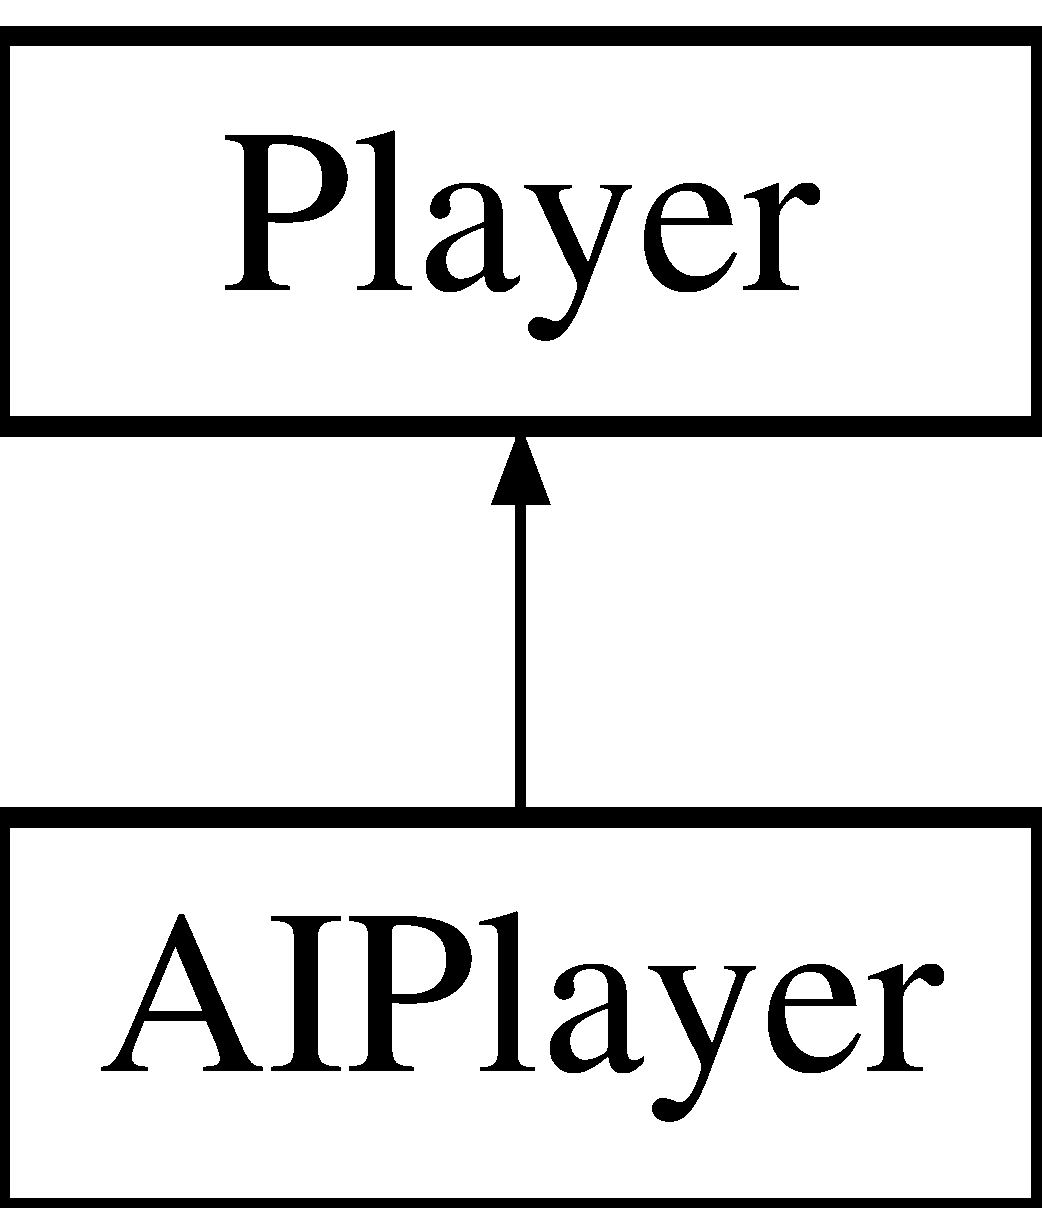
\includegraphics[height=2cm]{classAIPlayer}
\end{center}
\end{figure}
\subsection*{Public Member Functions}
\begin{DoxyCompactItemize}
\item 
\hyperlink{classAIPlayer_ae791562645a443fead734b4bdcb1509e}{AIPlayer} ()
\begin{DoxyCompactList}\small\item\em creates a \hyperlink{classAIPlayer}{AIPlayer} object for \hyperlink{classAIPlayer}{AIPlayer} class \item\end{DoxyCompactList}\item 
string \hyperlink{classAIPlayer_aaa733d49ac2e937a25d53a3b238fb3a8}{getName} ()
\item 
void \hyperlink{classAIPlayer_adb32c66ce4ba140188676aeea0317d36}{nextMove} (\hyperlink{classBoard}{Board} b)
\begin{DoxyCompactList}\small\item\em creates a move for \hyperlink{classBoard}{Board} \item\end{DoxyCompactList}\item 
\hyperlink{classMemento}{Memento} \hyperlink{classAIPlayer_a83d0865c5869bbf02a66207976842de6}{generateMemento} ()
\begin{DoxyCompactList}\small\item\em Generates a \hyperlink{classMemento}{Memento} object. \item\end{DoxyCompactList}\item 
void \hyperlink{classAIPlayer_a41aa8bd7a1d09ba00f1e6fa65083a248}{restoreMemento} (\hyperlink{classMemento}{Memento} memento)
\begin{DoxyCompactList}\small\item\em Restores this \hyperlink{classRegisteredPlayer}{RegisteredPlayer} object from the \hyperlink{classMemento}{Memento} object. \item\end{DoxyCompactList}\end{DoxyCompactItemize}


\subsection{Detailed Description}
a class for \hyperlink{classAIPlayer}{AIPlayer} .h \begin{DoxyAuthor}{Author}
Zackery Shortt 
\end{DoxyAuthor}
\begin{DoxyDate}{Date}
October 27, 2014 
\end{DoxyDate}


\subsection{Constructor \& Destructor Documentation}
\hypertarget{classAIPlayer_ae791562645a443fead734b4bdcb1509e}{
\index{AIPlayer@{AIPlayer}!AIPlayer@{AIPlayer}}
\index{AIPlayer@{AIPlayer}!AIPlayer@{AIPlayer}}
\subsubsection[{AIPlayer}]{\setlength{\rightskip}{0pt plus 5cm}AIPlayer::AIPlayer ()\hspace{0.3cm}{\ttfamily  \mbox{[}inline\mbox{]}}}}
\label{classAIPlayer_ae791562645a443fead734b4bdcb1509e}


creates a \hyperlink{classAIPlayer}{AIPlayer} object for \hyperlink{classAIPlayer}{AIPlayer} class 
\begin{DoxyParams}{Parameters}
\item[\mbox{$\leftarrow$} {\em name}]The name of the AI \end{DoxyParams}


\subsection{Member Function Documentation}
\hypertarget{classAIPlayer_a83d0865c5869bbf02a66207976842de6}{
\index{AIPlayer@{AIPlayer}!generateMemento@{generateMemento}}
\index{generateMemento@{generateMemento}!AIPlayer@{AIPlayer}}
\subsubsection[{generateMemento}]{\setlength{\rightskip}{0pt plus 5cm}{\bf Memento} AIPlayer::generateMemento ()\hspace{0.3cm}{\ttfamily  \mbox{[}virtual\mbox{]}}}}
\label{classAIPlayer_a83d0865c5869bbf02a66207976842de6}


Generates a \hyperlink{classMemento}{Memento} object. \begin{DoxyReturn}{Returns}
returns a memento object 
\end{DoxyReturn}


Implements \hyperlink{classPlayer_ae0b947230fe2f09d96f273798f19cf0d}{Player}.\hypertarget{classAIPlayer_aaa733d49ac2e937a25d53a3b238fb3a8}{
\index{AIPlayer@{AIPlayer}!getName@{getName}}
\index{getName@{getName}!AIPlayer@{AIPlayer}}
\subsubsection[{getName}]{\setlength{\rightskip}{0pt plus 5cm}string AIPlayer::getName ()\hspace{0.3cm}{\ttfamily  \mbox{[}virtual\mbox{]}}}}
\label{classAIPlayer_aaa733d49ac2e937a25d53a3b238fb3a8}
\begin{DoxyReturn}{Returns}
returns the name of the AI 
\end{DoxyReturn}


Implements \hyperlink{classPlayer}{Player}.\hypertarget{classAIPlayer_adb32c66ce4ba140188676aeea0317d36}{
\index{AIPlayer@{AIPlayer}!nextMove@{nextMove}}
\index{nextMove@{nextMove}!AIPlayer@{AIPlayer}}
\subsubsection[{nextMove}]{\setlength{\rightskip}{0pt plus 5cm}void AIPlayer::nextMove ({\bf Board} {\em b})}}
\label{classAIPlayer_adb32c66ce4ba140188676aeea0317d36}


creates a move for \hyperlink{classBoard}{Board} 
\begin{DoxyParams}{Parameters}
\item[\mbox{$\leftarrow$} {\em This}]is the board that has a move \end{DoxyParams}
\hypertarget{classAIPlayer_a41aa8bd7a1d09ba00f1e6fa65083a248}{
\index{AIPlayer@{AIPlayer}!restoreMemento@{restoreMemento}}
\index{restoreMemento@{restoreMemento}!AIPlayer@{AIPlayer}}
\subsubsection[{restoreMemento}]{\setlength{\rightskip}{0pt plus 5cm}void AIPlayer::restoreMemento ({\bf Memento} {\em memento})}}
\label{classAIPlayer_a41aa8bd7a1d09ba00f1e6fa65083a248}


Restores this \hyperlink{classRegisteredPlayer}{RegisteredPlayer} object from the \hyperlink{classMemento}{Memento} object. 
\begin{DoxyParams}{Parameters}
\item[\mbox{$\leftarrow$} {\em memento}]the memento object to restore \end{DoxyParams}


The documentation for this class was generated from the following file:\begin{DoxyCompactItemize}
\item 
source/Players/AIPlayer.h\end{DoxyCompactItemize}

\hypertarget{classBishopMove}{
\section{BishopMove Class Reference}
\label{classBishopMove}\index{BishopMove@{BishopMove}}
}
Inheritance diagram for BishopMove::\begin{figure}[H]
\begin{center}
\leavevmode
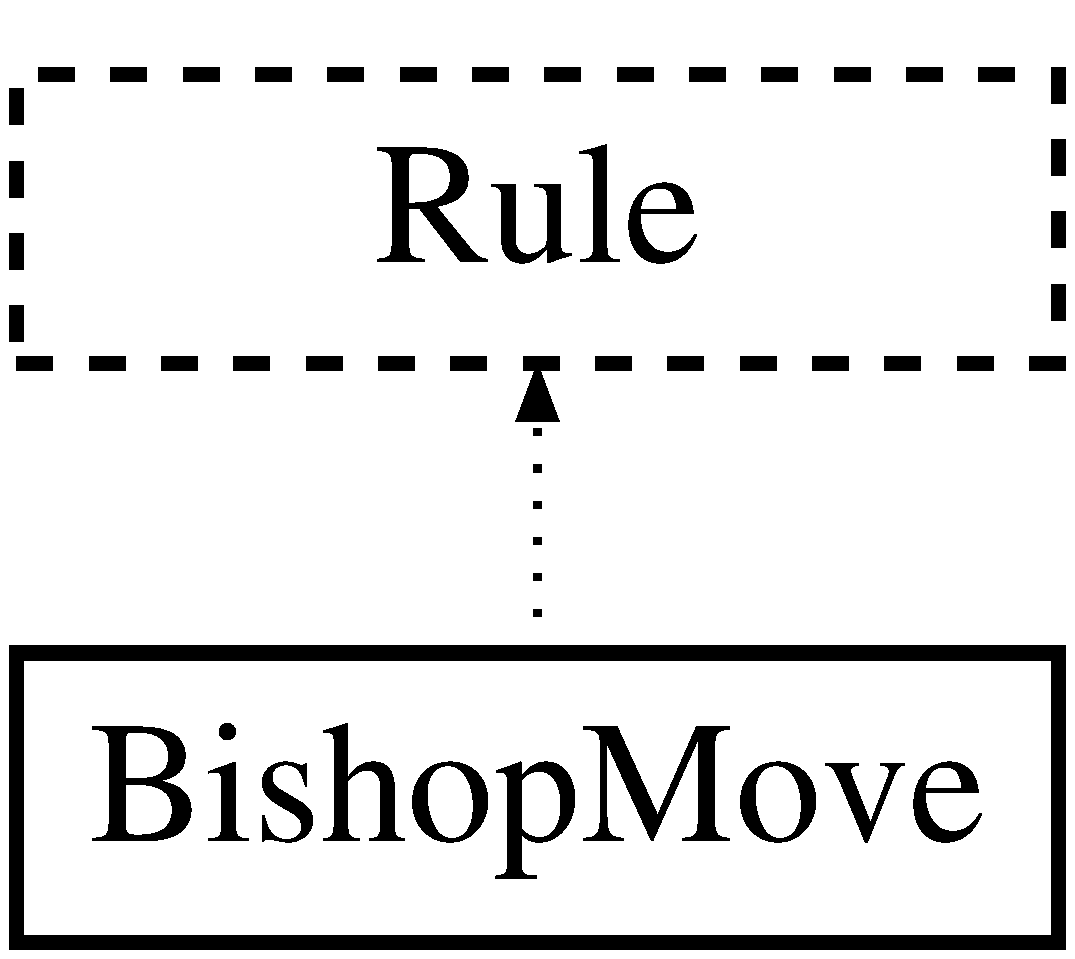
\includegraphics[height=2cm]{classBishopMove}
\end{center}
\end{figure}
\subsection*{Public Member Functions}
\begin{DoxyCompactItemize}
\item 
\hyperlink{classBishopMove_aa066339d2be626d650a7edde5d5ecfc1}{BishopMove} ()
\begin{DoxyCompactList}\small\item\em \hyperlink{classBishopMove}{BishopMove} creates a \hyperlink{classBishopMove}{BishopMove} object. \item\end{DoxyCompactList}\item 
int \hyperlink{classBishopMove_a30929c42136a677d9531d21696fd2c82}{validMove} (vector$<$ vector$<$ \hyperlink{classPiece}{Piece} $\ast$ $>$ $>$ \&b, int ix, int iy, int dx, int dy)
\begin{DoxyCompactList}\small\item\em validMove checks if the move made by the user is a valid move for bishop to make a perfect angle(ex. x+1,y+1). if valid calls pieceinway. if invalid return 0. \item\end{DoxyCompactList}\end{DoxyCompactItemize}


\subsection{Constructor \& Destructor Documentation}
\hypertarget{classBishopMove_aa066339d2be626d650a7edde5d5ecfc1}{
\index{BishopMove@{BishopMove}!BishopMove@{BishopMove}}
\index{BishopMove@{BishopMove}!BishopMove@{BishopMove}}
\subsubsection[{BishopMove}]{\setlength{\rightskip}{0pt plus 5cm}BishopMove::BishopMove ()}}
\label{classBishopMove_aa066339d2be626d650a7edde5d5ecfc1}


\hyperlink{classBishopMove}{BishopMove} creates a \hyperlink{classBishopMove}{BishopMove} object. 
\begin{DoxyParams}{Parameters}
\item[\mbox{$\leftarrow$} {\em b}]is a vector$<$ vector $<$ Piece$\ast$ $>$ $>$ object \item[\mbox{$\leftarrow$} {\em ix}]is the x for the initial location \item[\mbox{$\leftarrow$} {\em iy}]is the y for the initial location \item[\mbox{$\leftarrow$} {\em dx}]is the x for the destination location \item[\mbox{$\leftarrow$} {\em dy}]is the y for the destination location \end{DoxyParams}


\subsection{Member Function Documentation}
\hypertarget{classBishopMove_a30929c42136a677d9531d21696fd2c82}{
\index{BishopMove@{BishopMove}!validMove@{validMove}}
\index{validMove@{validMove}!BishopMove@{BishopMove}}
\subsubsection[{validMove}]{\setlength{\rightskip}{0pt plus 5cm}int BishopMove::validMove (vector$<$ vector$<$ {\bf Piece} $\ast$ $>$ $>$ \& {\em b}, \/  int {\em ix}, \/  int {\em iy}, \/  int {\em dx}, \/  int {\em dy})\hspace{0.3cm}{\ttfamily  \mbox{[}virtual\mbox{]}}}}
\label{classBishopMove_a30929c42136a677d9531d21696fd2c82}


validMove checks if the move made by the user is a valid move for bishop to make a perfect angle(ex. x+1,y+1). if valid calls pieceinway. if invalid return 0. \begin{DoxyReturn}{Returns}
an int 
\end{DoxyReturn}


Implements \hyperlink{classRule}{Rule}.

The documentation for this class was generated from the following files:\begin{DoxyCompactItemize}
\item 
source/Rules/\hyperlink{BishopMove_8h}{BishopMove.h}\item 
source/Rules/BishopMove.cc\end{DoxyCompactItemize}

\hypertarget{classBishopPiece}{
\section{BishopPiece Class Reference}
\label{classBishopPiece}\index{BishopPiece@{BishopPiece}}
}


a class for all Bishop Piece`s.  


{\ttfamily \#include $<$BishopPiece.h$>$}Inheritance diagram for BishopPiece::\begin{figure}[H]
\begin{center}
\leavevmode
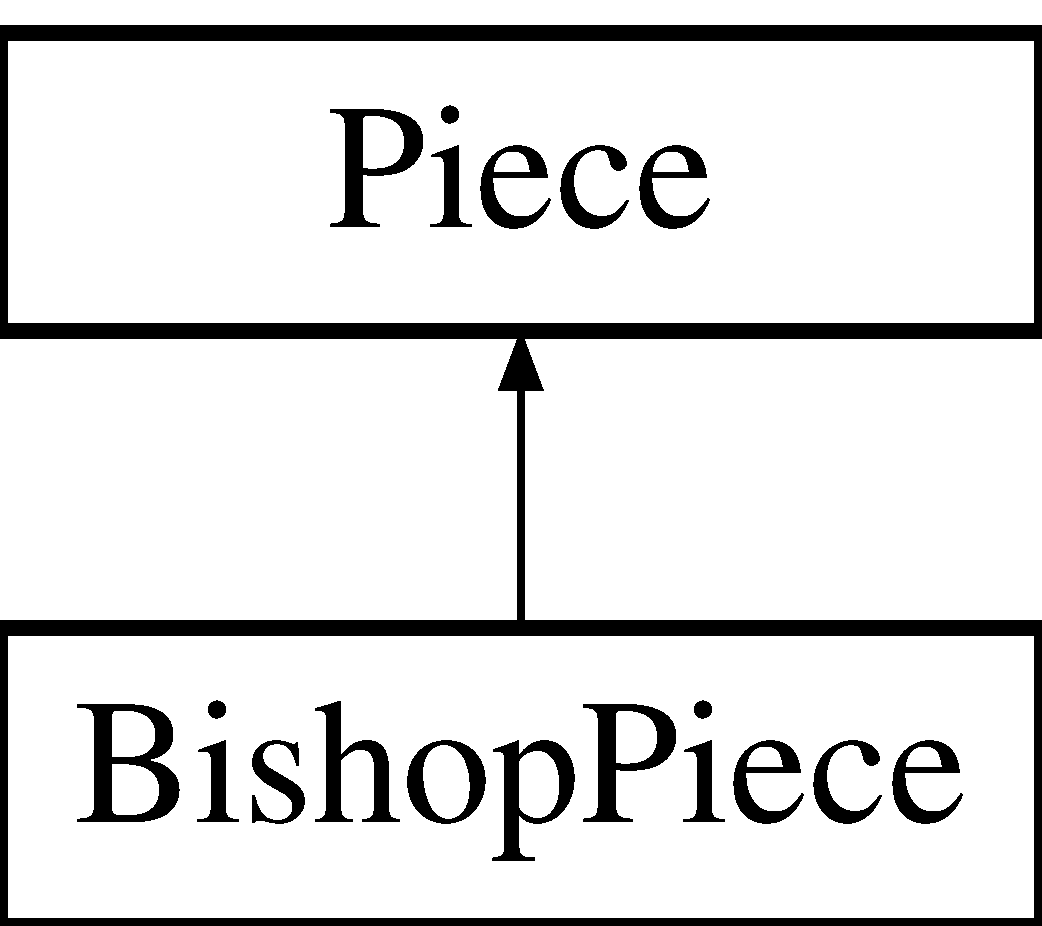
\includegraphics[height=2cm]{classBishopPiece}
\end{center}
\end{figure}
\subsection*{Public Member Functions}
\begin{DoxyCompactItemize}
\item 
\hypertarget{classBishopPiece_ae5bd27defc378a878b99d95d2d11d035}{
\hyperlink{classBishopPiece_ae5bd27defc378a878b99d95d2d11d035}{BishopPiece} (int c=0)}
\label{classBishopPiece_ae5bd27defc378a878b99d95d2d11d035}

\begin{DoxyCompactList}\small\item\em creates a \hyperlink{classPiece}{Piece} object \item\end{DoxyCompactList}\item 
int \hyperlink{classBishopPiece_ae40042d8edb9172b97955a1a3d651434}{getColor} () const 
\begin{DoxyCompactList}\small\item\em gets the color of the Bishop \hyperlink{classPiece}{Piece} \item\end{DoxyCompactList}\item 
void \hyperlink{classBishopPiece_ae75166e3d3bc71f3030268158cba4054}{setColor} (int colorOfPiece)
\begin{DoxyCompactList}\small\item\em sets the Color of the Bishop \hyperlink{classPiece}{Piece} \item\end{DoxyCompactList}\item 
string \hyperlink{classBishopPiece_af651439e984e4d28955db75da601b35b}{getType} () const 
\begin{DoxyCompactList}\small\item\em Returns Bishop to user. \item\end{DoxyCompactList}\item 
int \hyperlink{classBishopPiece_a0f0ed53268ba4b42c9e95a92a183d19d}{validMove} (vector$<$ vector$<$ \hyperlink{classPiece}{Piece} $\ast$ $>$ $>$ gameBoard, int ix, int iy, int dx, int dy)
\begin{DoxyCompactList}\small\item\em validates a move based on the Bishop rules. \item\end{DoxyCompactList}\end{DoxyCompactItemize}


\subsection{Detailed Description}
a class for all Bishop Piece`s. 

\subsection{Member Function Documentation}
\hypertarget{classBishopPiece_ae40042d8edb9172b97955a1a3d651434}{
\index{BishopPiece@{BishopPiece}!getColor@{getColor}}
\index{getColor@{getColor}!BishopPiece@{BishopPiece}}
\subsubsection[{getColor}]{\setlength{\rightskip}{0pt plus 5cm}int BishopPiece::getColor () const\hspace{0.3cm}{\ttfamily  \mbox{[}virtual\mbox{]}}}}
\label{classBishopPiece_ae40042d8edb9172b97955a1a3d651434}


gets the color of the Bishop \hyperlink{classPiece}{Piece} \begin{DoxyReturn}{Returns}
int a 0 if white and 1 if black 
\end{DoxyReturn}


Implements \hyperlink{classPiece_a1376072d4815719e60253ce5688df95c}{Piece}.\hypertarget{classBishopPiece_af651439e984e4d28955db75da601b35b}{
\index{BishopPiece@{BishopPiece}!getType@{getType}}
\index{getType@{getType}!BishopPiece@{BishopPiece}}
\subsubsection[{getType}]{\setlength{\rightskip}{0pt plus 5cm}string BishopPiece::getType () const\hspace{0.3cm}{\ttfamily  \mbox{[}virtual\mbox{]}}}}
\label{classBishopPiece_af651439e984e4d28955db75da601b35b}


Returns Bishop to user. \begin{DoxyReturn}{Returns}
a string that will return Bishop Type. 
\end{DoxyReturn}


Implements \hyperlink{classPiece_a5b88fcd786bb30b345b24fbc3ab24ab9}{Piece}.\hypertarget{classBishopPiece_ae75166e3d3bc71f3030268158cba4054}{
\index{BishopPiece@{BishopPiece}!setColor@{setColor}}
\index{setColor@{setColor}!BishopPiece@{BishopPiece}}
\subsubsection[{setColor}]{\setlength{\rightskip}{0pt plus 5cm}void BishopPiece::setColor (int {\em colorOfPiece})\hspace{0.3cm}{\ttfamily  \mbox{[}virtual\mbox{]}}}}
\label{classBishopPiece_ae75166e3d3bc71f3030268158cba4054}


sets the Color of the Bishop \hyperlink{classPiece}{Piece} 
\begin{DoxyParams}{Parameters}
\item[\mbox{$\leftarrow$} {\em colorOfPiece}]sets the Pawn Piece`s color \end{DoxyParams}


Implements \hyperlink{classPiece_a1387cb503dca308ac1e3bbe38a70a073}{Piece}.\hypertarget{classBishopPiece_a0f0ed53268ba4b42c9e95a92a183d19d}{
\index{BishopPiece@{BishopPiece}!validMove@{validMove}}
\index{validMove@{validMove}!BishopPiece@{BishopPiece}}
\subsubsection[{validMove}]{\setlength{\rightskip}{0pt plus 5cm}int BishopPiece::validMove (vector$<$ vector$<$ {\bf Piece} $\ast$ $>$ $>$ {\em gameBoard}, \/  int {\em ix}, \/  int {\em iy}, \/  int {\em dx}, \/  int {\em dy})}}
\label{classBishopPiece_a0f0ed53268ba4b42c9e95a92a183d19d}


validates a move based on the Bishop rules. 
\begin{DoxyParams}{Parameters}
\item[\mbox{$\leftarrow$} {\em board}]A \hyperlink{classBoard}{Board} that will contain the currect board state \item[\mbox{$\leftarrow$} {\em ix}]A int that holds the x coordinate of where the piece is moving from \item[\mbox{$\leftarrow$} {\em iy}]A int that holds the y coordinate of where the piece is moving from \item[\mbox{$\leftarrow$} {\em dx}]A int that holds the x coordinate of where the piece is moving to \item[\mbox{$\leftarrow$} {\em dy}]A int that holds the y coordinate of where the piece is moving to \end{DoxyParams}


The documentation for this class was generated from the following files:\begin{DoxyCompactItemize}
\item 
source/Piece/\hyperlink{BishopPiece_8h}{BishopPiece.h}\item 
source/Piece/BishopPiece.cc\end{DoxyCompactItemize}

\hypertarget{classBoard}{
\section{Board Class Reference}
\label{classBoard}\index{Board@{Board}}
}


a concrete class for creating a board which games will be played on.  


{\ttfamily \#include $<$Board.h$>$}\subsection*{Public Member Functions}
\begin{DoxyCompactItemize}
\item 
\hypertarget{classBoard_a8bbcd997b4099120e7427e06fd6a103f}{
\hyperlink{classBoard_a8bbcd997b4099120e7427e06fd6a103f}{Board} (int h=8, int w=8)}
\label{classBoard_a8bbcd997b4099120e7427e06fd6a103f}

\begin{DoxyCompactList}\small\item\em Creates a \hyperlink{classBoard}{Board} object. As well as declaires vector of Piece`s that will be on the board. \item\end{DoxyCompactList}\item 
\hypertarget{classBoard_af73f45730119a1fd8f6670f53f959e68}{
\hyperlink{classBoard_af73f45730119a1fd8f6670f53f959e68}{$\sim$Board} ()}
\label{classBoard_af73f45730119a1fd8f6670f53f959e68}

\begin{DoxyCompactList}\small\item\em Removes all the Piece`s that where on the board. \item\end{DoxyCompactList}\item 
\hyperlink{classPiece}{Piece} $\ast$ \hyperlink{classBoard_a80649196225f3e7da030b56a9bf19f64}{getPiece} (int x, int y)
\begin{DoxyCompactList}\small\item\em Given a x and y coordinate and return the piece that is on that square. \item\end{DoxyCompactList}\item 
void \hyperlink{classBoard_a4eca4cabd2a51a2095917b203fecbe0c}{setPiece} (int x, int y, \hyperlink{classPiece}{Piece} $\ast$p)
\begin{DoxyCompactList}\small\item\em gets player 2's id \item\end{DoxyCompactList}\item 
\hypertarget{classBoard_a888c8ce1bb6a4cede9fc54070de91fe5}{
void {\bfseries setNull} (int x, int y)}
\label{classBoard_a888c8ce1bb6a4cede9fc54070de91fe5}

\item 
void \hyperlink{classBoard_a7f35e7488ab3d4a72ebb34c56e3b3ec2}{setHeight} (int newHeight)
\begin{DoxyCompactList}\small\item\em sets the height of the \hyperlink{classBoard}{Board} to one provided by the user \item\end{DoxyCompactList}\item 
int \hyperlink{classBoard_a14466e56568d523e5f4d0d695ccbcce1}{getHeight} ()
\begin{DoxyCompactList}\small\item\em gets the height of the \hyperlink{classBoard}{Board} to one provided by the user \item\end{DoxyCompactList}\item 
int \hyperlink{classBoard_a67905f3b441a8605aeb50d8978415aa0}{getWidth} ()
\begin{DoxyCompactList}\small\item\em returns the width of the \hyperlink{classBoard}{Board} \item\end{DoxyCompactList}\item 
void \hyperlink{classBoard_ac1aed85ab99701f68b89d91c225a5ba7}{setWidth} (int newWidth)
\begin{DoxyCompactList}\small\item\em tsets the width of the \hyperlink{classBoard}{Board} to one provided by the user \item\end{DoxyCompactList}\item 
int \hyperlink{classBoard_a0f7aae004483872ecf3c1056ca961fef}{movePiece} (int ix, int iy, int dx, int dy)
\begin{DoxyCompactList}\small\item\em validates a move based on the Pieces Move attribute. This will be overwritten \item\end{DoxyCompactList}\item 
\hypertarget{classBoard_afafbabafdea2ea02d8d6bc57deb68ef9}{
void {\bfseries MoveHistory} (int cur1=0, int cur2=0, int des1=0, int des2=0, bool onOrOff=false)}
\label{classBoard_afafbabafdea2ea02d8d6bc57deb68ef9}

\item 
\hypertarget{classBoard_a74077081ee6423bf1022ffa68bddb9b5}{
vector$<$ string $>$ {\bfseries getBoardHistory} ()}
\label{classBoard_a74077081ee6423bf1022ffa68bddb9b5}

\end{DoxyCompactItemize}


\subsection{Detailed Description}
a concrete class for creating a board which games will be played on. 

\subsection{Member Function Documentation}
\hypertarget{classBoard_a14466e56568d523e5f4d0d695ccbcce1}{
\index{Board@{Board}!getHeight@{getHeight}}
\index{getHeight@{getHeight}!Board@{Board}}
\subsubsection[{getHeight}]{\setlength{\rightskip}{0pt plus 5cm}int Board::getHeight ()}}
\label{classBoard_a14466e56568d523e5f4d0d695ccbcce1}


gets the height of the \hyperlink{classBoard}{Board} to one provided by the user 
\begin{DoxyParams}{Parameters}
\item[\mbox{$\leftarrow$} {\em newHeight}]a new height which the board will be set to \end{DoxyParams}
\hypertarget{classBoard_a80649196225f3e7da030b56a9bf19f64}{
\index{Board@{Board}!getPiece@{getPiece}}
\index{getPiece@{getPiece}!Board@{Board}}
\subsubsection[{getPiece}]{\setlength{\rightskip}{0pt plus 5cm}{\bf Piece}$\ast$ Board::getPiece (int {\em x}, \/  int {\em y})}}
\label{classBoard_a80649196225f3e7da030b56a9bf19f64}


Given a x and y coordinate and return the piece that is on that square. 
\begin{DoxyParams}{Parameters}
\item[\mbox{$\leftarrow$} {\em x}]A int that contains the x coordinate \item[\mbox{$\leftarrow$} {\em y}]A int that contains the y coordinate \end{DoxyParams}
\begin{DoxyReturn}{Returns}
a \hyperlink{classPiece}{Piece} that is currently on the x and y square 
\end{DoxyReturn}
\hypertarget{classBoard_a67905f3b441a8605aeb50d8978415aa0}{
\index{Board@{Board}!getWidth@{getWidth}}
\index{getWidth@{getWidth}!Board@{Board}}
\subsubsection[{getWidth}]{\setlength{\rightskip}{0pt plus 5cm}int Board::getWidth ()}}
\label{classBoard_a67905f3b441a8605aeb50d8978415aa0}


returns the width of the \hyperlink{classBoard}{Board} \begin{DoxyReturn}{Returns}
the width of the \hyperlink{classBoard}{Board} 
\end{DoxyReturn}
\hypertarget{classBoard_a0f7aae004483872ecf3c1056ca961fef}{
\index{Board@{Board}!movePiece@{movePiece}}
\index{movePiece@{movePiece}!Board@{Board}}
\subsubsection[{movePiece}]{\setlength{\rightskip}{0pt plus 5cm}int Board::movePiece (int {\em ix}, \/  int {\em iy}, \/  int {\em dx}, \/  int {\em dy})}}
\label{classBoard_a0f7aae004483872ecf3c1056ca961fef}


validates a move based on the Pieces Move attribute. This will be overwritten 
\begin{DoxyParams}{Parameters}
\item[\mbox{$\leftarrow$} {\em board}]A \hyperlink{classBoard}{Board} that will contain the currect board state \item[\mbox{$\leftarrow$} {\em ix}]A int that holds the x coordinate of where the piece is moving from \item[\mbox{$\leftarrow$} {\em iy}]A int that holds the y coordinate of where the piece is moving from \item[\mbox{$\leftarrow$} {\em dx}]A int that holds the x coordinate of where the piece is moving to \item[\mbox{$\leftarrow$} {\em dy}]A int that holds the y coordinate of where the piece is moving to \end{DoxyParams}
\hypertarget{classBoard_a7f35e7488ab3d4a72ebb34c56e3b3ec2}{
\index{Board@{Board}!setHeight@{setHeight}}
\index{setHeight@{setHeight}!Board@{Board}}
\subsubsection[{setHeight}]{\setlength{\rightskip}{0pt plus 5cm}void Board::setHeight (int {\em newHeight})}}
\label{classBoard_a7f35e7488ab3d4a72ebb34c56e3b3ec2}


sets the height of the \hyperlink{classBoard}{Board} to one provided by the user 
\begin{DoxyParams}{Parameters}
\item[\mbox{$\leftarrow$} {\em newHeight}]a new height which the board will be set to \end{DoxyParams}
\hypertarget{classBoard_a4eca4cabd2a51a2095917b203fecbe0c}{
\index{Board@{Board}!setPiece@{setPiece}}
\index{setPiece@{setPiece}!Board@{Board}}
\subsubsection[{setPiece}]{\setlength{\rightskip}{0pt plus 5cm}void Board::setPiece (int {\em x}, \/  int {\em y}, \/  {\bf Piece} $\ast$ {\em p})}}
\label{classBoard_a4eca4cabd2a51a2095917b203fecbe0c}


gets player 2's id 
\begin{DoxyParams}{Parameters}
\item[\mbox{$\leftarrow$} {\em x}]A int that contains the x coordinate \item[\mbox{$\leftarrow$} {\em y}]A int that contains the y coordinate \item[\mbox{$\leftarrow$} {\em p}]A \hyperlink{classPiece}{Piece} that will be inserted \end{DoxyParams}
\begin{DoxyReturn}{Returns}
if the insert was successful 
\end{DoxyReturn}
\hypertarget{classBoard_ac1aed85ab99701f68b89d91c225a5ba7}{
\index{Board@{Board}!setWidth@{setWidth}}
\index{setWidth@{setWidth}!Board@{Board}}
\subsubsection[{setWidth}]{\setlength{\rightskip}{0pt plus 5cm}void Board::setWidth (int {\em newWidth})}}
\label{classBoard_ac1aed85ab99701f68b89d91c225a5ba7}


tsets the width of the \hyperlink{classBoard}{Board} to one provided by the user 
\begin{DoxyParams}{Parameters}
\item[\mbox{$\leftarrow$} {\em newWidth}]a new width which the board will be set to \end{DoxyParams}


The documentation for this class was generated from the following files:\begin{DoxyCompactItemize}
\item 
source/\hyperlink{Board_8h}{Board.h}\item 
source/Board.cc\end{DoxyCompactItemize}

\hypertarget{classCastlingMove}{
\section{CastlingMove Class Reference}
\label{classCastlingMove}\index{CastlingMove@{CastlingMove}}
}
Inheritance diagram for CastlingMove::\begin{figure}[H]
\begin{center}
\leavevmode
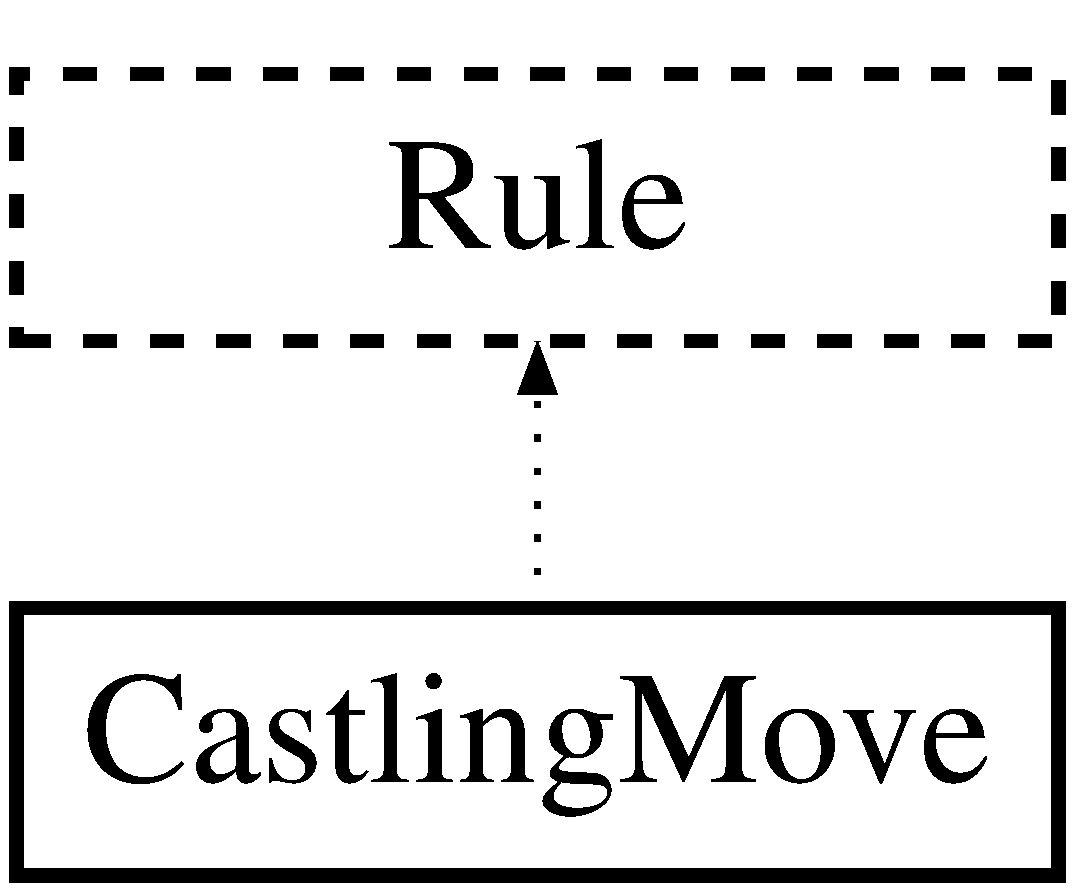
\includegraphics[height=2cm]{classCastlingMove}
\end{center}
\end{figure}
\subsection*{Public Member Functions}
\begin{DoxyCompactItemize}
\item 
\hyperlink{classCastlingMove_ac2b171638597ff26944c2426c35768de}{CastlingMove} ()
\begin{DoxyCompactList}\small\item\em \hyperlink{classCastlingMove}{CastlingMove} creates a \hyperlink{classCastlingMove}{CastlingMove} object. \item\end{DoxyCompactList}\item 
int \hyperlink{classCastlingMove_ad716f6021188a950d53b824bcdfdcb0d}{validMove} (vector$<$ vector$<$ \hyperlink{classPiece}{Piece} $\ast$ $>$ $>$ \&b, int ix, int iy, int dx, int dy)
\begin{DoxyCompactList}\small\item\em validMove checks if the king is moved two squares towards a rock. if its not F the move made by the user is a valid move that sacrifices the Castling rule. if valid calls \hyperlink{classPieceInWay}{PieceInWay}. if invalid return 0. \item\end{DoxyCompactList}\end{DoxyCompactItemize}


\subsection{Constructor \& Destructor Documentation}
\hypertarget{classCastlingMove_ac2b171638597ff26944c2426c35768de}{
\index{CastlingMove@{CastlingMove}!CastlingMove@{CastlingMove}}
\index{CastlingMove@{CastlingMove}!CastlingMove@{CastlingMove}}
\subsubsection[{CastlingMove}]{\setlength{\rightskip}{0pt plus 5cm}CastlingMove::CastlingMove ()}}
\label{classCastlingMove_ac2b171638597ff26944c2426c35768de}


\hyperlink{classCastlingMove}{CastlingMove} creates a \hyperlink{classCastlingMove}{CastlingMove} object. 
\begin{DoxyParams}{Parameters}
\item[\mbox{$\leftarrow$} {\em b}]is a vector$<$ vector $<$ Piece$\ast$ $>$ $>$ object \item[\mbox{$\leftarrow$} {\em ix}]is the x for the initial location \item[\mbox{$\leftarrow$} {\em iy}]is the y for the initial location \item[\mbox{$\leftarrow$} {\em dx}]is the x for the destination location \item[\mbox{$\leftarrow$} {\em dy}]is the y for the destination location \end{DoxyParams}


\subsection{Member Function Documentation}
\hypertarget{classCastlingMove_ad716f6021188a950d53b824bcdfdcb0d}{
\index{CastlingMove@{CastlingMove}!validMove@{validMove}}
\index{validMove@{validMove}!CastlingMove@{CastlingMove}}
\subsubsection[{validMove}]{\setlength{\rightskip}{0pt plus 5cm}int CastlingMove::validMove (vector$<$ vector$<$ {\bf Piece} $\ast$ $>$ $>$ \& {\em b}, \/  int {\em ix}, \/  int {\em iy}, \/  int {\em dx}, \/  int {\em dy})\hspace{0.3cm}{\ttfamily  \mbox{[}virtual\mbox{]}}}}
\label{classCastlingMove_ad716f6021188a950d53b824bcdfdcb0d}


validMove checks if the king is moved two squares towards a rock. if its not F the move made by the user is a valid move that sacrifices the Castling rule. if valid calls \hyperlink{classPieceInWay}{PieceInWay}. if invalid return 0. \begin{DoxyReturn}{Returns}
an int 
\end{DoxyReturn}


Implements \hyperlink{classRule}{Rule}.

The documentation for this class was generated from the following files:\begin{DoxyCompactItemize}
\item 
source/Rules/\hyperlink{CastlingMove_8h}{CastlingMove.h}\item 
source/Rules/CastlingMove.cc\end{DoxyCompactItemize}

\hypertarget{classChat}{
\section{Chat Class Reference}
\label{classChat}\index{Chat@{Chat}}
}


a concrete class for chat functionality between players.  


{\ttfamily \#include $<$Chat.h$>$}\subsection*{Public Member Functions}
\begin{DoxyCompactItemize}
\item 
\hyperlink{classChat_abc23d9c9b254089b8f486bd0ef6bc225}{Chat} (string playerOneId=\char`\"{}guest\char`\"{}, string playerTwoId=\char`\"{}guest\char`\"{})
\begin{DoxyCompactList}\small\item\em creates a \hyperlink{classChat}{Chat} object \item\end{DoxyCompactList}\item 
string \hyperlink{classChat_add2a099a2c259d0a4a7e88061a3ac7df}{getPlayerOneId} () const 
\begin{DoxyCompactList}\small\item\em gets player 1's id \item\end{DoxyCompactList}\item 
string \hyperlink{classChat_a017261b95b8794213381c1534881968b}{getPlayerTwoId} () const 
\begin{DoxyCompactList}\small\item\em gets player 2's id \item\end{DoxyCompactList}\item 
void \hyperlink{classChat_adbe497560146ca9d5a940792b407f9fc}{setPlayerOneId} (string playerOneId)
\begin{DoxyCompactList}\small\item\em sets \hyperlink{classPlayer}{Player} 1's Id \item\end{DoxyCompactList}\item 
void \hyperlink{classChat_ae81fb0422bd13afef5a18836d6c24a78}{setPlayerTwoId} (string playerTwoId)
\begin{DoxyCompactList}\small\item\em sets \hyperlink{classPlayer}{Player} 2's Id \item\end{DoxyCompactList}\item 
void \hyperlink{classChat_a02ce14db9d4c1c1aa7f5cb40df16eb60}{postMessage} (string name, string message)
\begin{DoxyCompactList}\small\item\em adds a new message \item\end{DoxyCompactList}\item 
vector$<$ pair$<$ string, string $>$ $>$ \& \hyperlink{classChat_a238969ca251c9fdd893b4466e6dea8ba}{getMessages} ()
\begin{DoxyCompactList}\small\item\em gets a reference to vector of messages \item\end{DoxyCompactList}\end{DoxyCompactItemize}


\subsection{Detailed Description}
a concrete class for chat functionality between players. 

\subsection{Constructor \& Destructor Documentation}
\hypertarget{classChat_abc23d9c9b254089b8f486bd0ef6bc225}{
\index{Chat@{Chat}!Chat@{Chat}}
\index{Chat@{Chat}!Chat@{Chat}}
\subsubsection[{Chat}]{\setlength{\rightskip}{0pt plus 5cm}Chat::Chat (string {\em playerOneId} = {\ttfamily \char`\"{}guest\char`\"{}}, \/  string {\em playerTwoId} = {\ttfamily \char`\"{}guest\char`\"{}})}}
\label{classChat_abc23d9c9b254089b8f486bd0ef6bc225}


creates a \hyperlink{classChat}{Chat} object 
\begin{DoxyParams}{Parameters}
\item[\mbox{$\leftarrow$} {\em playerOneId}]A string that is the id of player 1 \item[\mbox{$\leftarrow$} {\em playerTwoId}]A string that is the id of player 2 \end{DoxyParams}


\subsection{Member Function Documentation}
\hypertarget{classChat_a238969ca251c9fdd893b4466e6dea8ba}{
\index{Chat@{Chat}!getMessages@{getMessages}}
\index{getMessages@{getMessages}!Chat@{Chat}}
\subsubsection[{getMessages}]{\setlength{\rightskip}{0pt plus 5cm}string \& Chat::getMessages ()}}
\label{classChat_a238969ca251c9fdd893b4466e6dea8ba}


gets a reference to vector of messages \begin{DoxyReturn}{Returns}
A reference to a vector of pairs that stores the messages 
\end{DoxyReturn}
\hypertarget{classChat_add2a099a2c259d0a4a7e88061a3ac7df}{
\index{Chat@{Chat}!getPlayerOneId@{getPlayerOneId}}
\index{getPlayerOneId@{getPlayerOneId}!Chat@{Chat}}
\subsubsection[{getPlayerOneId}]{\setlength{\rightskip}{0pt plus 5cm}string Chat::getPlayerOneId () const}}
\label{classChat_add2a099a2c259d0a4a7e88061a3ac7df}


gets player 1's id \begin{DoxyReturn}{Returns}
player 1's id as a string 
\end{DoxyReturn}
\hypertarget{classChat_a017261b95b8794213381c1534881968b}{
\index{Chat@{Chat}!getPlayerTwoId@{getPlayerTwoId}}
\index{getPlayerTwoId@{getPlayerTwoId}!Chat@{Chat}}
\subsubsection[{getPlayerTwoId}]{\setlength{\rightskip}{0pt plus 5cm}string Chat::getPlayerTwoId () const}}
\label{classChat_a017261b95b8794213381c1534881968b}


gets player 2's id \begin{DoxyReturn}{Returns}
player 2's id as a string 
\end{DoxyReturn}
\hypertarget{classChat_a02ce14db9d4c1c1aa7f5cb40df16eb60}{
\index{Chat@{Chat}!postMessage@{postMessage}}
\index{postMessage@{postMessage}!Chat@{Chat}}
\subsubsection[{postMessage}]{\setlength{\rightskip}{0pt plus 5cm}void Chat::postMessage (string {\em name}, \/  string {\em message})}}
\label{classChat_a02ce14db9d4c1c1aa7f5cb40df16eb60}


adds a new message 
\begin{DoxyParams}{Parameters}
\item[\mbox{$\leftarrow$} {\em a}]pair of strings that is the player id and the message to be posted \end{DoxyParams}
\hypertarget{classChat_adbe497560146ca9d5a940792b407f9fc}{
\index{Chat@{Chat}!setPlayerOneId@{setPlayerOneId}}
\index{setPlayerOneId@{setPlayerOneId}!Chat@{Chat}}
\subsubsection[{setPlayerOneId}]{\setlength{\rightskip}{0pt plus 5cm}void Chat::setPlayerOneId (string {\em playerOneId})}}
\label{classChat_adbe497560146ca9d5a940792b407f9fc}


sets \hyperlink{classPlayer}{Player} 1's Id 
\begin{DoxyParams}{Parameters}
\item[\mbox{$\leftarrow$} {\em playerOneId}]A string that the id of player 1 is set to \end{DoxyParams}
\hypertarget{classChat_ae81fb0422bd13afef5a18836d6c24a78}{
\index{Chat@{Chat}!setPlayerTwoId@{setPlayerTwoId}}
\index{setPlayerTwoId@{setPlayerTwoId}!Chat@{Chat}}
\subsubsection[{setPlayerTwoId}]{\setlength{\rightskip}{0pt plus 5cm}void Chat::setPlayerTwoId (string {\em playerTwoId})}}
\label{classChat_ae81fb0422bd13afef5a18836d6c24a78}


sets \hyperlink{classPlayer}{Player} 2's Id 
\begin{DoxyParams}{Parameters}
\item[\mbox{$\leftarrow$} {\em playerTwoId}]A string that the id of player 2 is set to \end{DoxyParams}


The documentation for this class was generated from the following files:\begin{DoxyCompactItemize}
\item 
source/\hyperlink{Chat_8h}{Chat.h}\item 
source/Chat.cc\end{DoxyCompactItemize}

\hypertarget{classCheckTurn}{
\section{CheckTurn Class Reference}
\label{classCheckTurn}\index{CheckTurn@{CheckTurn}}
}
Inheritance diagram for CheckTurn::\begin{figure}[H]
\begin{center}
\leavevmode
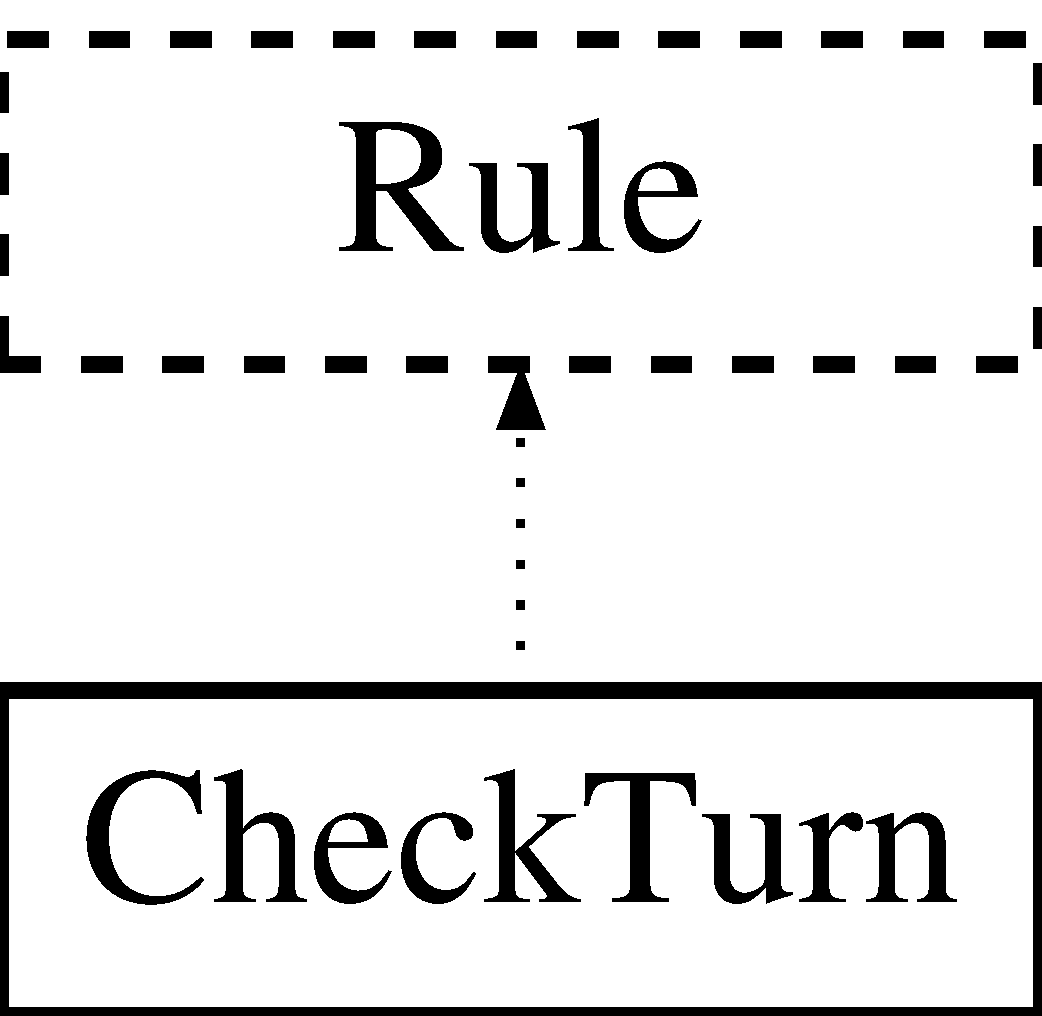
\includegraphics[height=2cm]{classCheckTurn}
\end{center}
\end{figure}
\subsection*{Public Member Functions}
\begin{DoxyCompactItemize}
\item 
\hyperlink{classCheckTurn_aedd0e9efd064863ae813f80e5847b197}{CheckTurn} ()
\begin{DoxyCompactList}\small\item\em \hyperlink{classCheckTurn}{CheckTurn} creates a \hyperlink{classCheckTurn}{CheckTurn} object. \item\end{DoxyCompactList}\item 
int \hyperlink{classCheckTurn_acb5d45e0ee242eb4af3dc6a7437b39e5}{validMove} (vector$<$ vector$<$ \hyperlink{classPiece}{Piece} $\ast$ $>$ $>$ \&b, int ix, int iy, int dx, int dy)
\begin{DoxyCompactList}\small\item\em validMove checks if the pieces left alive are the bishop and king or the knight and king it will return 2 else return 1. \item\end{DoxyCompactList}\end{DoxyCompactItemize}


\subsection{Constructor \& Destructor Documentation}
\hypertarget{classCheckTurn_aedd0e9efd064863ae813f80e5847b197}{
\index{CheckTurn@{CheckTurn}!CheckTurn@{CheckTurn}}
\index{CheckTurn@{CheckTurn}!CheckTurn@{CheckTurn}}
\subsubsection[{CheckTurn}]{\setlength{\rightskip}{0pt plus 5cm}CheckTurn::CheckTurn ()}}
\label{classCheckTurn_aedd0e9efd064863ae813f80e5847b197}


\hyperlink{classCheckTurn}{CheckTurn} creates a \hyperlink{classCheckTurn}{CheckTurn} object. 
\begin{DoxyParams}{Parameters}
\item[\mbox{$\leftarrow$} {\em b}]is a vector$<$ vector $<$ Piece$\ast$ $>$ $>$ object \item[\mbox{$\leftarrow$} {\em ix}]is the x for the initial location \item[\mbox{$\leftarrow$} {\em iy}]is the y for the initial location \item[\mbox{$\leftarrow$} {\em dx}]is the x for the destination location \item[\mbox{$\leftarrow$} {\em dy}]is the y for the destination location \end{DoxyParams}


\subsection{Member Function Documentation}
\hypertarget{classCheckTurn_acb5d45e0ee242eb4af3dc6a7437b39e5}{
\index{CheckTurn@{CheckTurn}!validMove@{validMove}}
\index{validMove@{validMove}!CheckTurn@{CheckTurn}}
\subsubsection[{validMove}]{\setlength{\rightskip}{0pt plus 5cm}int CheckTurn::validMove (vector$<$ vector$<$ {\bf Piece} $\ast$ $>$ $>$ \& {\em b}, \/  int {\em ix}, \/  int {\em iy}, \/  int {\em dx}, \/  int {\em dy})\hspace{0.3cm}{\ttfamily  \mbox{[}virtual\mbox{]}}}}
\label{classCheckTurn_acb5d45e0ee242eb4af3dc6a7437b39e5}


validMove checks if the pieces left alive are the bishop and king or the knight and king it will return 2 else return 1. \begin{DoxyReturn}{Returns}
an int 
\end{DoxyReturn}


Implements \hyperlink{classRule}{Rule}.

The documentation for this class was generated from the following files:\begin{DoxyCompactItemize}
\item 
source/Rules/\hyperlink{CheckTurn_8h}{CheckTurn.h}\item 
source/Rules/CheckTurn.cc\end{DoxyCompactItemize}

\hypertarget{classChessBoard}{
\section{ChessBoard Class Reference}
\label{classChessBoard}\index{ChessBoard@{ChessBoard}}
}


a concrete class for creating a chess board which games will be played on.  


{\ttfamily \#include $<$ChessBoard.h$>$}\subsection*{Public Member Functions}
\begin{DoxyCompactItemize}
\item 
\hypertarget{classChessBoard_a6585395bb4f064b4f4566df1c7fa4276}{
\hyperlink{classChessBoard_a6585395bb4f064b4f4566df1c7fa4276}{ChessBoard} ()}
\label{classChessBoard_a6585395bb4f064b4f4566df1c7fa4276}

\begin{DoxyCompactList}\small\item\em Creates a chess \hyperlink{classBoard}{Board} object. \item\end{DoxyCompactList}\item 
\hypertarget{classChessBoard_a76c7d0672aac47763c93414169170393}{
void {\bfseries setUpChessBoard} ()}
\label{classChessBoard_a76c7d0672aac47763c93414169170393}

\item 
bool \hyperlink{classChessBoard_a88cc4b18d8ff152040bbf19f3938f263}{undo} (string str=\char`\"{}delete later\char`\"{})
\begin{DoxyCompactList}\small\item\em undo`s to the previouse move on the board \item\end{DoxyCompactList}\item 
vector$<$ \hyperlink{classPiece}{Piece} $\ast$ $>$ \hyperlink{classChessBoard_a213f4676d46d0c938cdf4cbdf9e89fc6}{getDeadBoard} ()
\begin{DoxyCompactList}\small\item\em returns the dead \hyperlink{classBoard}{Board} \item\end{DoxyCompactList}\item 
void \hyperlink{classChessBoard_a3d378451fd54b5f335d32143a413afaf}{setDeadBoard} (\hyperlink{classPiece}{Piece} $\ast$p)
\begin{DoxyCompactList}\small\item\em sets the DeadBoard \item\end{DoxyCompactList}\item 
\hypertarget{classChessBoard_ace11797096bfed610192baf5a26631ab}{
\hyperlink{classPiece}{Piece} $\ast$ {\bfseries getPiece} (int row, int col)}
\label{classChessBoard_ace11797096bfed610192baf5a26631ab}

\item 
\hypertarget{classChessBoard_a2cb0e5de6cef36be60fe00bd27aed712}{
\hyperlink{classPiece}{Piece} $\ast$ {\bfseries popDeadBoard} ()}
\label{classChessBoard_a2cb0e5de6cef36be60fe00bd27aed712}

\item 
int \hyperlink{classChessBoard_a1764e3d94bee2cc7a1ce6b03ae818b61}{movePiece} (int ix, int iy, int dx, int dy)
\begin{DoxyCompactList}\small\item\em validates a move based on the Pieces Move attribute. \item\end{DoxyCompactList}\item 
\hypertarget{classChessBoard_aa36755cd28d9426554ab80d0f3a337a5}{
vector$<$ string $>$ {\bfseries getGameHistory} ()}
\label{classChessBoard_aa36755cd28d9426554ab80d0f3a337a5}

\end{DoxyCompactItemize}


\subsection{Detailed Description}
a concrete class for creating a chess board which games will be played on. 

\subsection{Member Function Documentation}
\hypertarget{classChessBoard_a213f4676d46d0c938cdf4cbdf9e89fc6}{
\index{ChessBoard@{ChessBoard}!getDeadBoard@{getDeadBoard}}
\index{getDeadBoard@{getDeadBoard}!ChessBoard@{ChessBoard}}
\subsubsection[{getDeadBoard}]{\setlength{\rightskip}{0pt plus 5cm}vector$<$ {\bf Piece} $\ast$ $>$ ChessBoard::getDeadBoard ()}}
\label{classChessBoard_a213f4676d46d0c938cdf4cbdf9e89fc6}


returns the dead \hyperlink{classBoard}{Board} \begin{DoxyReturn}{Returns}
the dead \hyperlink{classBoard}{Board} 
\end{DoxyReturn}
\hypertarget{classChessBoard_a1764e3d94bee2cc7a1ce6b03ae818b61}{
\index{ChessBoard@{ChessBoard}!movePiece@{movePiece}}
\index{movePiece@{movePiece}!ChessBoard@{ChessBoard}}
\subsubsection[{movePiece}]{\setlength{\rightskip}{0pt plus 5cm}int ChessBoard::movePiece (int {\em ix}, \/  int {\em iy}, \/  int {\em dx}, \/  int {\em dy})}}
\label{classChessBoard_a1764e3d94bee2cc7a1ce6b03ae818b61}


validates a move based on the Pieces Move attribute. 
\begin{DoxyParams}{Parameters}
\item[\mbox{$\leftarrow$} {\em board}]A \hyperlink{classBoard}{Board} that will contain the currect board state \item[\mbox{$\leftarrow$} {\em ix}]A int that holds the x coordinate of where the piece is moving from \item[\mbox{$\leftarrow$} {\em iy}]A int that holds the y coordinate of where the piece is moving from \item[\mbox{$\leftarrow$} {\em dx}]A int that holds the x coordinate of where the piece is moving to \item[\mbox{$\leftarrow$} {\em dy}]A int that holds the y coordinate of where the piece is moving to \end{DoxyParams}
\hypertarget{classChessBoard_a3d378451fd54b5f335d32143a413afaf}{
\index{ChessBoard@{ChessBoard}!setDeadBoard@{setDeadBoard}}
\index{setDeadBoard@{setDeadBoard}!ChessBoard@{ChessBoard}}
\subsubsection[{setDeadBoard}]{\setlength{\rightskip}{0pt plus 5cm}void ChessBoard::setDeadBoard ({\bf Piece} $\ast$ {\em p})}}
\label{classChessBoard_a3d378451fd54b5f335d32143a413afaf}


sets the DeadBoard 
\begin{DoxyParams}{Parameters}
\item[\mbox{$\leftarrow$} {\em b}]sets a new dead \hyperlink{classBoard}{Board} \end{DoxyParams}
\hypertarget{classChessBoard_a88cc4b18d8ff152040bbf19f3938f263}{
\index{ChessBoard@{ChessBoard}!undo@{undo}}
\index{undo@{undo}!ChessBoard@{ChessBoard}}
\subsubsection[{undo}]{\setlength{\rightskip}{0pt plus 5cm}bool ChessBoard::undo (string {\em str} = {\ttfamily \char`\"{}delete~later\char`\"{}})}}
\label{classChessBoard_a88cc4b18d8ff152040bbf19f3938f263}


undo`s to the previouse move on the board \begin{DoxyReturn}{Returns}
the previose board state 
\end{DoxyReturn}


The documentation for this class was generated from the following files:\begin{DoxyCompactItemize}
\item 
source/\hyperlink{ChessBoard_8h}{ChessBoard.h}\item 
source/ChessBoard.cc\end{DoxyCompactItemize}

\hypertarget{classChessGame}{
\section{ChessGame Class Reference}
\label{classChessGame}\index{ChessGame@{ChessGame}}
}


a class for \hyperlink{classGame}{Game}  


{\ttfamily \#include $<$ChessGame.h$>$}Inheritance diagram for ChessGame::\begin{figure}[H]
\begin{center}
\leavevmode
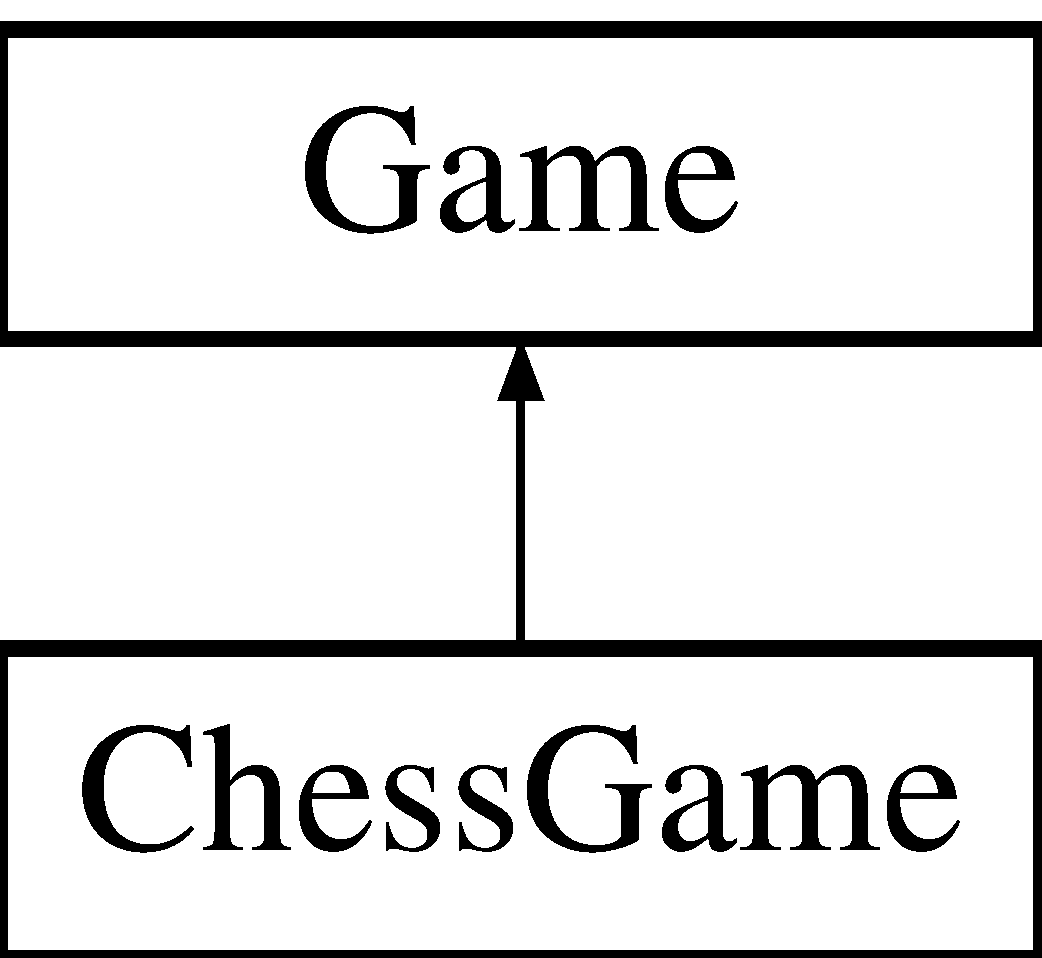
\includegraphics[height=2cm]{classChessGame}
\end{center}
\end{figure}
\subsection*{Public Member Functions}
\begin{DoxyCompactItemize}
\item 
\hyperlink{classChessGame_a7c9d1caa97c7ca5737f187a6066662b2}{ChessGame} ()
\begin{DoxyCompactList}\small\item\em Creates a \hyperlink{classChessGame}{ChessGame}. \item\end{DoxyCompactList}\item 
\hypertarget{classChessGame_a9c7f4475dcd31ab4e1f98f033fb0c60f}{
\hyperlink{classChessGame_a9c7f4475dcd31ab4e1f98f033fb0c60f}{$\sim$ChessGame} ()}
\label{classChessGame_a9c7f4475dcd31ab4e1f98f033fb0c60f}

\begin{DoxyCompactList}\small\item\em destructor for \hyperlink{classChessGame}{ChessGame}. \item\end{DoxyCompactList}\item 
\hyperlink{classBoard}{Board} $\ast$ \hyperlink{classChessGame_aae64a8ad5e54881d22d17a63cbc3159d}{getDeadBoard} ()
\begin{DoxyCompactList}\small\item\em This function returns a pointer to board. \item\end{DoxyCompactList}\item 
bool \hyperlink{classChessGame_af39a867cb667ca6befdab8cddb48ea3e}{setDeadBoard} (\hyperlink{classBoard}{Board} b)
\begin{DoxyCompactList}\small\item\em sets board \item\end{DoxyCompactList}\item 
bool \hyperlink{classChessGame_a19ce1ce19741d65888e60d741f658394}{undo} ()
\begin{DoxyCompactList}\small\item\em undo a move \item\end{DoxyCompactList}\item 
const vector$<$ string $>$ $\ast$ \hyperlink{classChessGame_a4a6bd9631a46b9f59b6d1b619e743a1a}{getGameHistory} ()
\begin{DoxyCompactList}\small\item\em gets a pointer to game history \item\end{DoxyCompactList}\item 
void \hyperlink{classChessGame_ae91e34d3cff8c49c243d2a5f6164b4b6}{addMove} (string move)
\begin{DoxyCompactList}\small\item\em adds a move to game history \item\end{DoxyCompactList}\item 
deadHistory $\ast$ \hyperlink{classChessGame_a60066cc951dc9fa90e850dc8b57ab210}{getDeadHistory} ()
\begin{DoxyCompactList}\small\item\em gets a pointer to deadHistory \item\end{DoxyCompactList}\end{DoxyCompactItemize}


\subsection{Detailed Description}
a class for \hyperlink{classGame}{Game} .h \begin{DoxyAuthor}{Author}
Zackery Shortt 
\end{DoxyAuthor}
\begin{DoxyDate}{Date}
October 28, 2014 a class for \hyperlink{classChessGame}{ChessGame} based on the \hyperlink{classGame}{Game} class. 
\end{DoxyDate}


\subsection{Constructor \& Destructor Documentation}
\hypertarget{classChessGame_a7c9d1caa97c7ca5737f187a6066662b2}{
\index{ChessGame@{ChessGame}!ChessGame@{ChessGame}}
\index{ChessGame@{ChessGame}!ChessGame@{ChessGame}}
\subsubsection[{ChessGame}]{\setlength{\rightskip}{0pt plus 5cm}ChessGame::ChessGame ()}}
\label{classChessGame_a7c9d1caa97c7ca5737f187a6066662b2}


Creates a \hyperlink{classChessGame}{ChessGame}. a class for \hyperlink{classChessGame}{ChessGame}, inherits from \hyperlink{classGame}{Game}

.cc \begin{DoxyAuthor}{Author}
Zackery Shortt 
\end{DoxyAuthor}
\begin{DoxyDate}{Date}
November 14, 2014 
\end{DoxyDate}


\subsection{Member Function Documentation}
\hypertarget{classChessGame_ae91e34d3cff8c49c243d2a5f6164b4b6}{
\index{ChessGame@{ChessGame}!addMove@{addMove}}
\index{addMove@{addMove}!ChessGame@{ChessGame}}
\subsubsection[{addMove}]{\setlength{\rightskip}{0pt plus 5cm}void ChessGame::addMove (string {\em move})}}
\label{classChessGame_ae91e34d3cff8c49c243d2a5f6164b4b6}


adds a move to game history 
\begin{DoxyParams}{Parameters}
\item[\mbox{$\leftarrow$} {\em move}]The move to add \end{DoxyParams}
\hypertarget{classChessGame_aae64a8ad5e54881d22d17a63cbc3159d}{
\index{ChessGame@{ChessGame}!getDeadBoard@{getDeadBoard}}
\index{getDeadBoard@{getDeadBoard}!ChessGame@{ChessGame}}
\subsubsection[{getDeadBoard}]{\setlength{\rightskip}{0pt plus 5cm}{\bf Board} $\ast$ ChessGame::getDeadBoard ()}}
\label{classChessGame_aae64a8ad5e54881d22d17a63cbc3159d}


This function returns a pointer to board. \begin{DoxyReturn}{Returns}
returns a pointer to deadBoard 
\end{DoxyReturn}
\hypertarget{classChessGame_a60066cc951dc9fa90e850dc8b57ab210}{
\index{ChessGame@{ChessGame}!getDeadHistory@{getDeadHistory}}
\index{getDeadHistory@{getDeadHistory}!ChessGame@{ChessGame}}
\subsubsection[{getDeadHistory}]{\setlength{\rightskip}{0pt plus 5cm}deadHistory$\ast$ ChessGame::getDeadHistory ()}}
\label{classChessGame_a60066cc951dc9fa90e850dc8b57ab210}


gets a pointer to deadHistory \begin{DoxyReturn}{Returns}
returns a pointer to deadHistory 
\end{DoxyReturn}
\hypertarget{classChessGame_a4a6bd9631a46b9f59b6d1b619e743a1a}{
\index{ChessGame@{ChessGame}!getGameHistory@{getGameHistory}}
\index{getGameHistory@{getGameHistory}!ChessGame@{ChessGame}}
\subsubsection[{getGameHistory}]{\setlength{\rightskip}{0pt plus 5cm}const vector$<$ string $>$ $\ast$ ChessGame::getGameHistory ()}}
\label{classChessGame_a4a6bd9631a46b9f59b6d1b619e743a1a}


gets a pointer to game history \begin{DoxyReturn}{Returns}
returns a pointer to gameHistory 
\end{DoxyReturn}
\hypertarget{classChessGame_af39a867cb667ca6befdab8cddb48ea3e}{
\index{ChessGame@{ChessGame}!setDeadBoard@{setDeadBoard}}
\index{setDeadBoard@{setDeadBoard}!ChessGame@{ChessGame}}
\subsubsection[{setDeadBoard}]{\setlength{\rightskip}{0pt plus 5cm}bool ChessGame::setDeadBoard ({\bf Board} {\em b})}}
\label{classChessGame_af39a867cb667ca6befdab8cddb48ea3e}


sets board 
\begin{DoxyParams}{Parameters}
\item[\mbox{$\leftarrow$} {\em This}]is the \hyperlink{classBoard}{Board} that deadBoard will be set to \end{DoxyParams}
\begin{DoxyReturn}{Returns}
returns a bool whether it was successful 
\end{DoxyReturn}
\hypertarget{classChessGame_a19ce1ce19741d65888e60d741f658394}{
\index{ChessGame@{ChessGame}!undo@{undo}}
\index{undo@{undo}!ChessGame@{ChessGame}}
\subsubsection[{undo}]{\setlength{\rightskip}{0pt plus 5cm}bool ChessGame::undo ()}}
\label{classChessGame_a19ce1ce19741d65888e60d741f658394}


undo a move \begin{DoxyReturn}{Returns}
returns a bool whether it was successful 
\end{DoxyReturn}


The documentation for this class was generated from the following files:\begin{DoxyCompactItemize}
\item 
source/ChessGame.h\item 
source/ChessGame.cc\end{DoxyCompactItemize}

\hypertarget{classchessGameGUI}{
\section{chessGameGUI Class Reference}
\label{classchessGameGUI}\index{chessGameGUI@{chessGameGUI}}
}
Inheritance diagram for chessGameGUI::\begin{figure}[H]
\begin{center}
\leavevmode
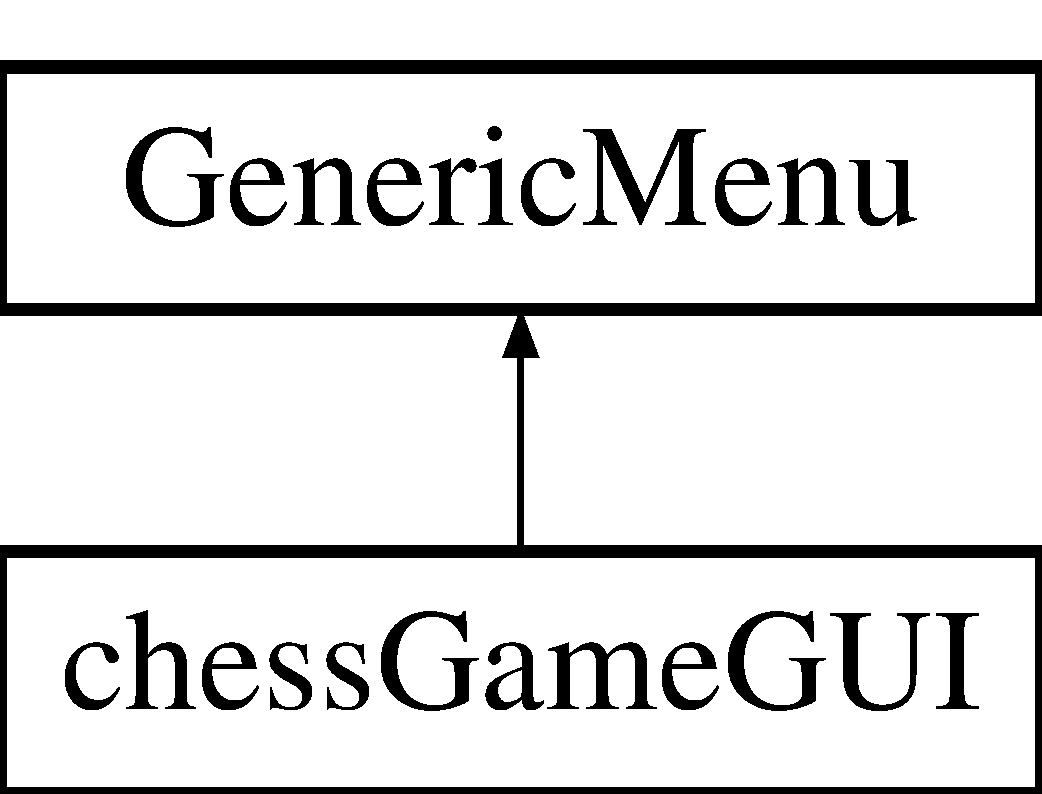
\includegraphics[height=2cm]{classchessGameGUI}
\end{center}
\end{figure}
\subsection*{Public Member Functions}
\begin{DoxyCompactItemize}
\item 
\hyperlink{classGenericMenu}{GenericMenu} $\ast$ \hyperlink{classchessGameGUI_afcafe4d3b432bae7cd8439b689886a8d}{menufunc} (string \&opt, \hyperlink{classstatus}{status} $\ast$\&info)
\begin{DoxyCompactList}\small\item\em menufunc is the general handler for implementing the functionality of this menu class \item\end{DoxyCompactList}\end{DoxyCompactItemize}


\subsection{Member Function Documentation}
\hypertarget{classchessGameGUI_afcafe4d3b432bae7cd8439b689886a8d}{
\index{chessGameGUI@{chessGameGUI}!menufunc@{menufunc}}
\index{menufunc@{menufunc}!chessGameGUI@{chessGameGUI}}
\subsubsection[{menufunc}]{\setlength{\rightskip}{0pt plus 5cm}{\bf GenericMenu} $\ast$ chessGameGUI::menufunc (string \& {\em opt}, \/  {\bf status} $\ast$\& {\em info})\hspace{0.3cm}{\ttfamily  \mbox{[}virtual\mbox{]}}}}
\label{classchessGameGUI_afcafe4d3b432bae7cd8439b689886a8d}


menufunc is the general handler for implementing the functionality of this menu class 
\begin{DoxyParams}{Parameters}
\item[\mbox{$\leftarrow$} {\em opt}]a reference for the program to decide where it must go in the main param\mbox{[}in\mbox{]} \hyperlink{classstatus}{status} is a class to enable manipulation of the current game and players between classes \end{DoxyParams}


Implements \hyperlink{classGenericMenu_a290ad7ec3331edc968190b1d7b48a397}{GenericMenu}.

The documentation for this class was generated from the following files:\begin{DoxyCompactItemize}
\item 
source/chessGameGUI.h\item 
source/chessGameGUI.cc\end{DoxyCompactItemize}

\hypertarget{classConsecutiveMove}{
\section{ConsecutiveMove Class Reference}
\label{classConsecutiveMove}\index{ConsecutiveMove@{ConsecutiveMove}}
}
Inheritance diagram for ConsecutiveMove::\begin{figure}[H]
\begin{center}
\leavevmode
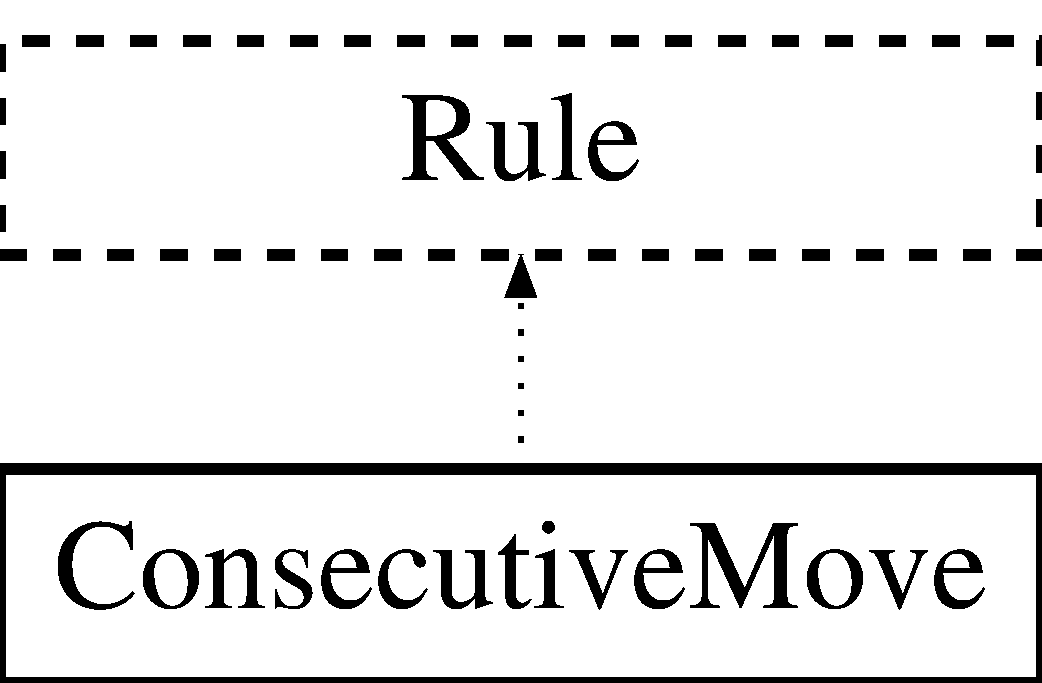
\includegraphics[height=2cm]{classConsecutiveMove}
\end{center}
\end{figure}
\subsection*{Public Member Functions}
\begin{DoxyCompactItemize}
\item 
\hyperlink{classConsecutiveMove_a46221ac47cb9051830e1799d5a29604e}{ConsecutiveMove} ()
\begin{DoxyCompactList}\small\item\em \hyperlink{classConsecutiveMove}{ConsecutiveMove} creates a \hyperlink{classConsecutiveMove}{ConsecutiveMove} object. \item\end{DoxyCompactList}\item 
\hypertarget{classConsecutiveMove_aa44597e9e07562a16042210fe1b9f090}{
int \hyperlink{classConsecutiveMove_aa44597e9e07562a16042210fe1b9f090}{validMove} (vector$<$ vector$<$ \hyperlink{classPiece}{Piece} $\ast$ $>$ $>$ \&b, int ix, int iy, int dx, int dy)}
\label{classConsecutiveMove_aa44597e9e07562a16042210fe1b9f090}

\begin{DoxyCompactList}\small\item\em validMove checks if the pieces left alive are the bishop and king or the knight and king it will return 2 else return 1. \item\end{DoxyCompactList}\end{DoxyCompactItemize}


\subsection{Constructor \& Destructor Documentation}
\hypertarget{classConsecutiveMove_a46221ac47cb9051830e1799d5a29604e}{
\index{ConsecutiveMove@{ConsecutiveMove}!ConsecutiveMove@{ConsecutiveMove}}
\index{ConsecutiveMove@{ConsecutiveMove}!ConsecutiveMove@{ConsecutiveMove}}
\subsubsection[{ConsecutiveMove}]{\setlength{\rightskip}{0pt plus 5cm}ConsecutiveMove::ConsecutiveMove ()}}
\label{classConsecutiveMove_a46221ac47cb9051830e1799d5a29604e}


\hyperlink{classConsecutiveMove}{ConsecutiveMove} creates a \hyperlink{classConsecutiveMove}{ConsecutiveMove} object. 
\begin{DoxyParams}{Parameters}
\item[\mbox{$\leftarrow$} {\em b}]is a vector$<$ vector $<$ Piece$\ast$ $>$ $>$ object \item[\mbox{$\leftarrow$} {\em ix}]is the x for the initial location \item[\mbox{$\leftarrow$} {\em iy}]is the y for the initial location \item[\mbox{$\leftarrow$} {\em dx}]is the x for the destination location \item[\mbox{$\leftarrow$} {\em dy}]is the y for the destination location \end{DoxyParams}


The documentation for this class was generated from the following files:\begin{DoxyCompactItemize}
\item 
source/Rules/\hyperlink{ConsecutiveMove_8h}{ConsecutiveMove.h}\item 
source/Rules/ConsecutiveMove.cc\end{DoxyCompactItemize}

\hypertarget{classDatabase}{
\section{Database Class Reference}
\label{classDatabase}\index{Database@{Database}}
}


a concrete class for database functionality for game programs.  


{\ttfamily \#include $<$Database.h$>$}\subsection*{Public Member Functions}
\begin{DoxyCompactItemize}
\item 
\hyperlink{classDatabase_af6c74356771bb4fab7f650c538b69082}{Database} (string directoryLocation=DATABASE\_\-LOCATION)
\begin{DoxyCompactList}\small\item\em creates a \hyperlink{classDatabase}{Database} object \item\end{DoxyCompactList}\item 
vector$<$ string $>$ \hyperlink{classDatabase_aefebb94db8894a40bd3fbd691c1d034c}{loadGame} (string gameName)
\begin{DoxyCompactList}\small\item\em loads a move by move play onto the gameHistory vector, then returns it. \item\end{DoxyCompactList}\item 
void \hyperlink{classDatabase_ab7769733153f13a11257401ed7b2bf23}{saveGame} (vector$<$ string $>$ gameHistory, string gameName)
\begin{DoxyCompactList}\small\item\em saves a vector of gameHistory to the gameName \item\end{DoxyCompactList}\item 
vector$<$ string $>$ \hyperlink{classDatabase_af77269e1ad834ae1d9d2e694cc5f6b7b}{getSaveList} ()
\begin{DoxyCompactList}\small\item\em returns the list of saved games found in the save game folder \item\end{DoxyCompactList}\item 
vector$<$ \hyperlink{classMemento}{Memento} $\ast$ $>$ \hyperlink{classDatabase_ae91622236a16acaf9d27ff73940f84f3}{getTopPlayers} (int playerNum=10)
\item 
void \hyperlink{classDatabase_a656673898e8f702a1b009c9c74d13b3e}{savePlayer} (\hyperlink{classMemento}{Memento} $\ast$playerMemento, string playerName)
\begin{DoxyCompactList}\small\item\em saves a memento object to given filename \item\end{DoxyCompactList}\item 
\hyperlink{classMemento}{Memento} $\ast$ \hyperlink{classDatabase_a635262537d097df45f6371966d9caefe}{loadPlayer} (string playerName)
\begin{DoxyCompactList}\small\item\em returns memento object of player \item\end{DoxyCompactList}\item 
void \hyperlink{classDatabase_aba5f0b5de3883729e5b0be7cf5b17b8c}{saveTournament} (\hyperlink{classTournament}{Tournament} tournament, string fileName)
\begin{DoxyCompactList}\small\item\em saves a \hyperlink{classTournament}{Tournament} to file \item\end{DoxyCompactList}\item 
map$<$ int, string $>$ \hyperlink{classDatabase_a1b403d4b38ea6c9d2e5d4d4b80f845db}{loadTournament} (string tournamentName)
\begin{DoxyCompactList}\small\item\em loads tournament from file \item\end{DoxyCompactList}\item 
\hypertarget{classDatabase_a96cc3743e82a8906424a74c366240277}{
bool {\bfseries doesPlayerExist} (string name)}
\label{classDatabase_a96cc3743e82a8906424a74c366240277}

\end{DoxyCompactItemize}


\subsection{Detailed Description}
a concrete class for database functionality for game programs. 

\subsection{Constructor \& Destructor Documentation}
\hypertarget{classDatabase_af6c74356771bb4fab7f650c538b69082}{
\index{Database@{Database}!Database@{Database}}
\index{Database@{Database}!Database@{Database}}
\subsubsection[{Database}]{\setlength{\rightskip}{0pt plus 5cm}Database::Database (string {\em directoryLocation} = {\ttfamily DATABASE\_\-LOCATION})}}
\label{classDatabase_af6c74356771bb4fab7f650c538b69082}


creates a \hyperlink{classDatabase}{Database} object 
\begin{DoxyParams}{Parameters}
\item[\mbox{$\leftarrow$} {\em directoryLocation}]the location of the directory that the files are stored in \end{DoxyParams}


\subsection{Member Function Documentation}
\hypertarget{classDatabase_af77269e1ad834ae1d9d2e694cc5f6b7b}{
\index{Database@{Database}!getSaveList@{getSaveList}}
\index{getSaveList@{getSaveList}!Database@{Database}}
\subsubsection[{getSaveList}]{\setlength{\rightskip}{0pt plus 5cm}vector$<$string$>$ Database::getSaveList ()}}
\label{classDatabase_af77269e1ad834ae1d9d2e694cc5f6b7b}


returns the list of saved games found in the save game folder \begin{DoxyReturn}{Returns}
a vector of strings containing the names of saved game files 
\end{DoxyReturn}
\hypertarget{classDatabase_ae91622236a16acaf9d27ff73940f84f3}{
\index{Database@{Database}!getTopPlayers@{getTopPlayers}}
\index{getTopPlayers@{getTopPlayers}!Database@{Database}}
\subsubsection[{getTopPlayers}]{\setlength{\rightskip}{0pt plus 5cm}vector$<${\bf Memento}$\ast$$>$ Database::getTopPlayers (int {\em playerNum} = {\ttfamily 10})}}
\label{classDatabase_ae91622236a16acaf9d27ff73940f84f3}
returns a vector of player Mementos containing the top “int” number of players 
\begin{DoxyParams}{Parameters}
\item[\mbox{$\leftarrow$} {\em playerNum}]an int containing the number of top players to return \end{DoxyParams}
\begin{DoxyReturn}{Returns}
a vector of player Memento's containing the top players in decreasing order 
\end{DoxyReturn}
\hypertarget{classDatabase_aefebb94db8894a40bd3fbd691c1d034c}{
\index{Database@{Database}!loadGame@{loadGame}}
\index{loadGame@{loadGame}!Database@{Database}}
\subsubsection[{loadGame}]{\setlength{\rightskip}{0pt plus 5cm}vector$<$string$>$ Database::loadGame (string {\em gameName})}}
\label{classDatabase_aefebb94db8894a40bd3fbd691c1d034c}


loads a move by move play onto the gameHistory vector, then returns it. 
\begin{DoxyParams}{Parameters}
\item[\mbox{$\leftarrow$} {\em gameName}]the name of the game file to be loaded in \end{DoxyParams}
\begin{DoxyReturn}{Returns}
a vector of strings containing the moves to be performed to restore game to previous state. (may also be used to replay game for replayPlayer) 
\end{DoxyReturn}
\hypertarget{classDatabase_a635262537d097df45f6371966d9caefe}{
\index{Database@{Database}!loadPlayer@{loadPlayer}}
\index{loadPlayer@{loadPlayer}!Database@{Database}}
\subsubsection[{loadPlayer}]{\setlength{\rightskip}{0pt plus 5cm}{\bf Memento}$\ast$ Database::loadPlayer (string {\em playerName})}}
\label{classDatabase_a635262537d097df45f6371966d9caefe}


returns memento object of player 
\begin{DoxyParams}{Parameters}
\item[\mbox{$\leftarrow$} {\em playerName}]a string of the player \end{DoxyParams}
\begin{DoxyReturn}{Returns}
a player memento object 
\end{DoxyReturn}
\hypertarget{classDatabase_a1b403d4b38ea6c9d2e5d4d4b80f845db}{
\index{Database@{Database}!loadTournament@{loadTournament}}
\index{loadTournament@{loadTournament}!Database@{Database}}
\subsubsection[{loadTournament}]{\setlength{\rightskip}{0pt plus 5cm}string Database::loadTournament (string {\em tournamentName})}}
\label{classDatabase_a1b403d4b38ea6c9d2e5d4d4b80f845db}


loads tournament from file 
\begin{DoxyParams}{Parameters}
\item[\mbox{$\leftarrow$} {\em tournamentName}]the filename to load \end{DoxyParams}
\begin{DoxyReturn}{Returns}
a map containing the rank of everyone in the tournament 
\end{DoxyReturn}
\hypertarget{classDatabase_ab7769733153f13a11257401ed7b2bf23}{
\index{Database@{Database}!saveGame@{saveGame}}
\index{saveGame@{saveGame}!Database@{Database}}
\subsubsection[{saveGame}]{\setlength{\rightskip}{0pt plus 5cm}void Database::saveGame (vector$<$ string $>$ {\em gameHistory}, \/  string {\em gameName})}}
\label{classDatabase_ab7769733153f13a11257401ed7b2bf23}


saves a vector of gameHistory to the gameName 
\begin{DoxyParams}{Parameters}
\item[\mbox{$\leftarrow$} {\em gameHistory}]a vector of strings containing the history of moves \item[\mbox{$\leftarrow$} {\em gameName}]a string containing the file name to save the game to \end{DoxyParams}
\hypertarget{classDatabase_a656673898e8f702a1b009c9c74d13b3e}{
\index{Database@{Database}!savePlayer@{savePlayer}}
\index{savePlayer@{savePlayer}!Database@{Database}}
\subsubsection[{savePlayer}]{\setlength{\rightskip}{0pt plus 5cm}void Database::savePlayer ({\bf Memento} $\ast$ {\em playerMemento}, \/  string {\em playerName})}}
\label{classDatabase_a656673898e8f702a1b009c9c74d13b3e}


saves a memento object to given filename 
\begin{DoxyParams}{Parameters}
\item[\mbox{$\leftarrow$} {\em a}]memento object of a player to save to file. \end{DoxyParams}
\hypertarget{classDatabase_aba5f0b5de3883729e5b0be7cf5b17b8c}{
\index{Database@{Database}!saveTournament@{saveTournament}}
\index{saveTournament@{saveTournament}!Database@{Database}}
\subsubsection[{saveTournament}]{\setlength{\rightskip}{0pt plus 5cm}void Database::saveTournament ({\bf Tournament} {\em tournament}, \/  string {\em fileName})}}
\label{classDatabase_aba5f0b5de3883729e5b0be7cf5b17b8c}


saves a \hyperlink{classTournament}{Tournament} to file 
\begin{DoxyParams}{Parameters}
\item[\mbox{$\leftarrow$} {\em tournament}]a tournament that is saved to file \item[\mbox{$\leftarrow$} {\em fileName}]the fileName to save the tournament to \end{DoxyParams}


The documentation for this class was generated from the following files:\begin{DoxyCompactItemize}
\item 
source/\hyperlink{Database_8h}{Database.h}\item 
source/Database.cc\end{DoxyCompactItemize}

\hypertarget{classdatabase__load__error}{
\section{database\_\-load\_\-error Class Reference}
\label{classdatabase__load__error}\index{database\_\-load\_\-error@{database\_\-load\_\-error}}
}
\subsection*{Public Member Functions}
\begin{DoxyCompactItemize}
\item 
\hyperlink{classdatabase__load__error_adfe936915a1470e830024c4278c68aa2}{database\_\-load\_\-error} (const std::string \&msg)
\begin{DoxyCompactList}\small\item\em Constructor for \hyperlink{classdatabase__load__error}{database\_\-load\_\-error} Class. \item\end{DoxyCompactList}\end{DoxyCompactItemize}


\subsection{Constructor \& Destructor Documentation}
\hypertarget{classdatabase__load__error_adfe936915a1470e830024c4278c68aa2}{
\index{database\_\-load\_\-error@{database\_\-load\_\-error}!database\_\-load\_\-error@{database\_\-load\_\-error}}
\index{database\_\-load\_\-error@{database\_\-load\_\-error}!database_load_error@{database\_\-load\_\-error}}
\subsubsection[{database\_\-load\_\-error}]{\setlength{\rightskip}{0pt plus 5cm}database\_\-load\_\-error::database\_\-load\_\-error (const std::string \& {\em msg})\hspace{0.3cm}{\ttfamily  \mbox{[}inline\mbox{]}}}}
\label{classdatabase__load__error_adfe936915a1470e830024c4278c68aa2}


Constructor for \hyperlink{classdatabase__load__error}{database\_\-load\_\-error} Class. This is the Constructor for the \hyperlink{classdatabase__load__error}{database\_\-load\_\-error} class. 
\begin{DoxyParams}{Parameters}
\item[\mbox{$\leftarrow$} {\em msg}]The error message for the exception \end{DoxyParams}


The documentation for this class was generated from the following file:\begin{DoxyCompactItemize}
\item 
source/\hyperlink{Errors_8h}{Errors.h}\end{DoxyCompactItemize}

\hypertarget{classEmptyPiece}{
\section{EmptyPiece Class Reference}
\label{classEmptyPiece}\index{EmptyPiece@{EmptyPiece}}
}


a class for all Pawn Piece`s.  


{\ttfamily \#include $<$EmptyPiece.h$>$}Inheritance diagram for EmptyPiece::\begin{figure}[H]
\begin{center}
\leavevmode
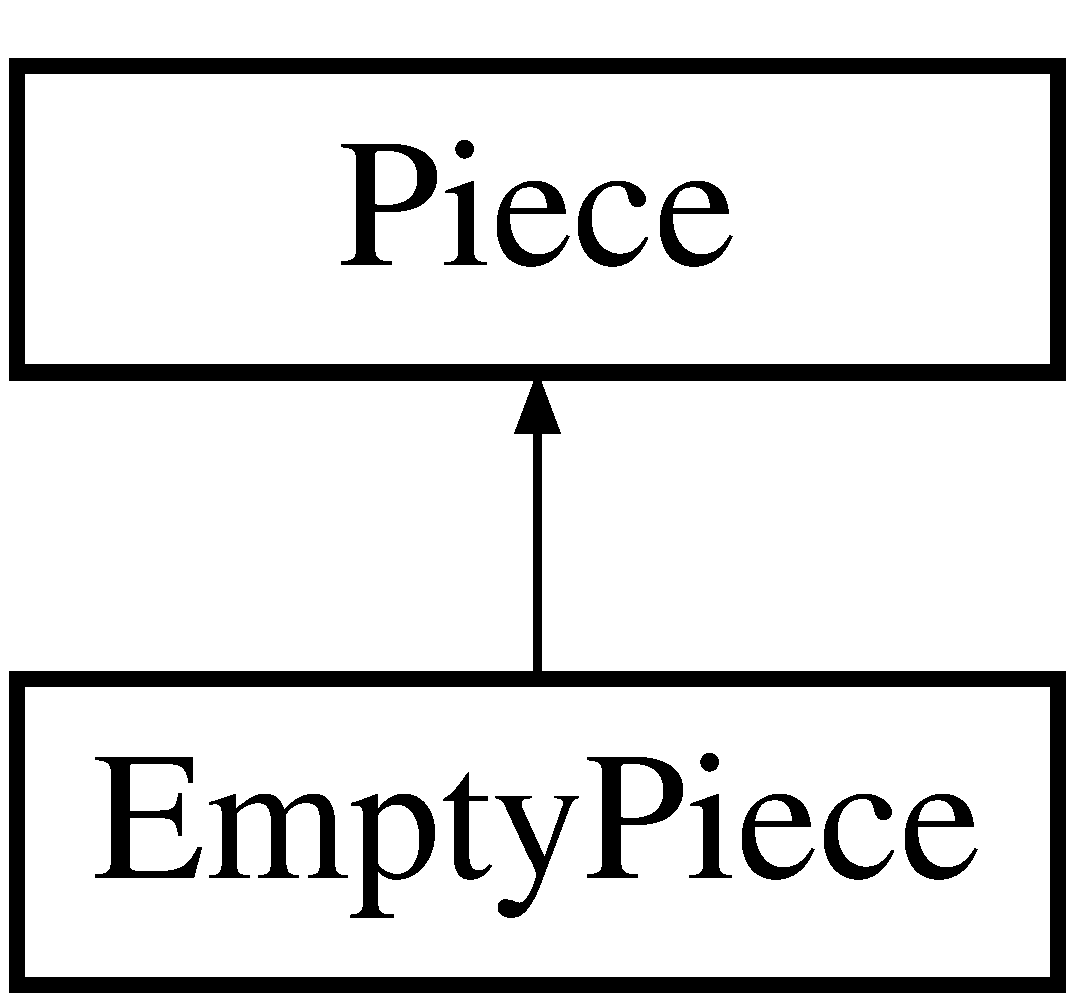
\includegraphics[height=2cm]{classEmptyPiece}
\end{center}
\end{figure}
\subsection*{Public Member Functions}
\begin{DoxyCompactItemize}
\item 
\hypertarget{classEmptyPiece_add461e061d61e0b8129fb2d079b1b599}{
\hyperlink{classEmptyPiece_add461e061d61e0b8129fb2d079b1b599}{EmptyPiece} (int c=3)}
\label{classEmptyPiece_add461e061d61e0b8129fb2d079b1b599}

\begin{DoxyCompactList}\small\item\em creates a \hyperlink{classPiece}{Piece} object \item\end{DoxyCompactList}\item 
int \hyperlink{classEmptyPiece_aa0ae8e05e0471cf05e17bc9f56e30188}{getColor} () const 
\begin{DoxyCompactList}\small\item\em gets the color of the Pawn \hyperlink{classPiece}{Piece} \item\end{DoxyCompactList}\item 
void \hyperlink{classEmptyPiece_ae46e7ddf6275c1508528e06929cf2660}{setColor} (int colorOfPiece)
\begin{DoxyCompactList}\small\item\em sets the Color of the Pawn \hyperlink{classPiece}{Piece} \item\end{DoxyCompactList}\item 
string \hyperlink{classEmptyPiece_ad71f9165591337d5df65c4f2500e2d36}{getType} () const 
\begin{DoxyCompactList}\small\item\em Returns Pawn to user. \item\end{DoxyCompactList}\item 
virtual int \hyperlink{classEmptyPiece_a198d7e2fd83b5564a569f580b6ccd69f}{validMove} (vector$<$ vector$<$ \hyperlink{classPiece}{Piece} $\ast$ $>$ $>$ gameBoard, int ix, int iy, int dx, int dy)
\begin{DoxyCompactList}\small\item\em validates a move based on the Pawn rules. \item\end{DoxyCompactList}\end{DoxyCompactItemize}


\subsection{Detailed Description}
a class for all Pawn Piece`s. 

\subsection{Member Function Documentation}
\hypertarget{classEmptyPiece_aa0ae8e05e0471cf05e17bc9f56e30188}{
\index{EmptyPiece@{EmptyPiece}!getColor@{getColor}}
\index{getColor@{getColor}!EmptyPiece@{EmptyPiece}}
\subsubsection[{getColor}]{\setlength{\rightskip}{0pt plus 5cm}int EmptyPiece::getColor () const\hspace{0.3cm}{\ttfamily  \mbox{[}virtual\mbox{]}}}}
\label{classEmptyPiece_aa0ae8e05e0471cf05e17bc9f56e30188}


gets the color of the Pawn \hyperlink{classPiece}{Piece} \begin{DoxyReturn}{Returns}
int a 0 if white and 1 if black 
\end{DoxyReturn}


Implements \hyperlink{classPiece_a1376072d4815719e60253ce5688df95c}{Piece}.\hypertarget{classEmptyPiece_ad71f9165591337d5df65c4f2500e2d36}{
\index{EmptyPiece@{EmptyPiece}!getType@{getType}}
\index{getType@{getType}!EmptyPiece@{EmptyPiece}}
\subsubsection[{getType}]{\setlength{\rightskip}{0pt plus 5cm}string EmptyPiece::getType () const\hspace{0.3cm}{\ttfamily  \mbox{[}virtual\mbox{]}}}}
\label{classEmptyPiece_ad71f9165591337d5df65c4f2500e2d36}


Returns Pawn to user. \begin{DoxyReturn}{Returns}
a string that will return Pawn Type. 
\end{DoxyReturn}


Implements \hyperlink{classPiece_a5b88fcd786bb30b345b24fbc3ab24ab9}{Piece}.\hypertarget{classEmptyPiece_ae46e7ddf6275c1508528e06929cf2660}{
\index{EmptyPiece@{EmptyPiece}!setColor@{setColor}}
\index{setColor@{setColor}!EmptyPiece@{EmptyPiece}}
\subsubsection[{setColor}]{\setlength{\rightskip}{0pt plus 5cm}void EmptyPiece::setColor (int {\em colorOfPiece})\hspace{0.3cm}{\ttfamily  \mbox{[}virtual\mbox{]}}}}
\label{classEmptyPiece_ae46e7ddf6275c1508528e06929cf2660}


sets the Color of the Pawn \hyperlink{classPiece}{Piece} 
\begin{DoxyParams}{Parameters}
\item[\mbox{$\leftarrow$} {\em colorOfPiece}]sets the Pawn Piece`s color \end{DoxyParams}


Implements \hyperlink{classPiece_a1387cb503dca308ac1e3bbe38a70a073}{Piece}.\hypertarget{classEmptyPiece_a198d7e2fd83b5564a569f580b6ccd69f}{
\index{EmptyPiece@{EmptyPiece}!validMove@{validMove}}
\index{validMove@{validMove}!EmptyPiece@{EmptyPiece}}
\subsubsection[{validMove}]{\setlength{\rightskip}{0pt plus 5cm}virtual int EmptyPiece::validMove (vector$<$ vector$<$ {\bf Piece} $\ast$ $>$ $>$ {\em gameBoard}, \/  int {\em ix}, \/  int {\em iy}, \/  int {\em dx}, \/  int {\em dy})\hspace{0.3cm}{\ttfamily  \mbox{[}virtual\mbox{]}}}}
\label{classEmptyPiece_a198d7e2fd83b5564a569f580b6ccd69f}


validates a move based on the Pawn rules. 
\begin{DoxyParams}{Parameters}
\item[\mbox{$\leftarrow$} {\em board}]A \hyperlink{classBoard}{Board} that will contain the currect board state \item[\mbox{$\leftarrow$} {\em ix}]A int that holds the x coordinate of where the piece is moving from \item[\mbox{$\leftarrow$} {\em iy}]A int that holds the y coordinate of where the piece is moving from \item[\mbox{$\leftarrow$} {\em dx}]A int that holds the x coordinate of where the piece is moving to \item[\mbox{$\leftarrow$} {\em dy}]A int that holds the y coordinate of where the piece is moving to \end{DoxyParams}


The documentation for this class was generated from the following files:\begin{DoxyCompactItemize}
\item 
source/Piece/\hyperlink{EmptyPiece_8h}{EmptyPiece.h}\item 
source/Piece/EmptyPiece.cc\end{DoxyCompactItemize}

\hypertarget{classEndMenu}{
\section{EndMenu Class Reference}
\label{classEndMenu}\index{EndMenu@{EndMenu}}
}


\hyperlink{classEndMenu}{EndMenu} is a subclass of \hyperlink{classGenericMenu}{GenericMenu}.  


{\ttfamily \#include $<$EndMenu.h$>$}Inheritance diagram for EndMenu::\begin{figure}[H]
\begin{center}
\leavevmode
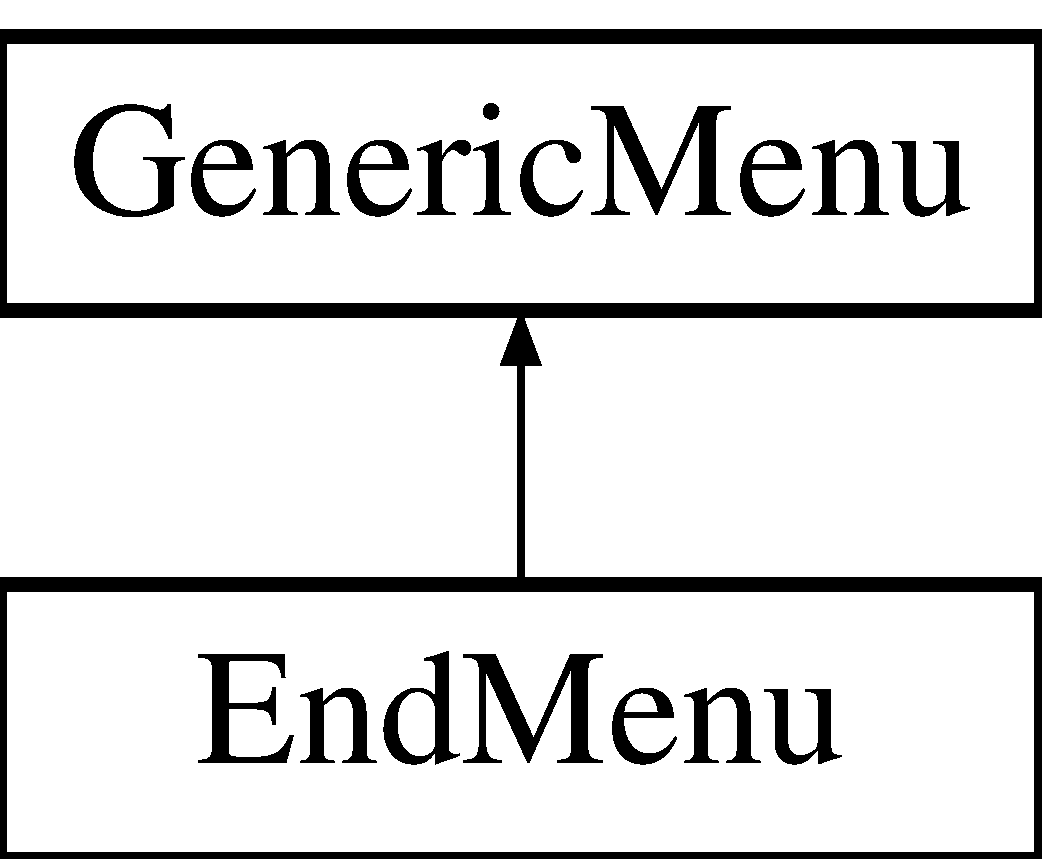
\includegraphics[height=2cm]{classEndMenu}
\end{center}
\end{figure}
\subsection*{Public Member Functions}
\begin{DoxyCompactItemize}
\item 
\hyperlink{classGenericMenu}{GenericMenu} $\ast$ \hyperlink{classEndMenu_a8fc10a35897496066f1db862bad44028}{menufunc} (string \&opt, \hyperlink{classstatus}{status} $\ast$\&info)
\begin{DoxyCompactList}\small\item\em menufunc is the general handler for implementing the functionality of this menu class \item\end{DoxyCompactList}\end{DoxyCompactItemize}


\subsection{Detailed Description}
\hyperlink{classEndMenu}{EndMenu} is a subclass of \hyperlink{classGenericMenu}{GenericMenu}. 

\subsection{Member Function Documentation}
\hypertarget{classEndMenu_a8fc10a35897496066f1db862bad44028}{
\index{EndMenu@{EndMenu}!menufunc@{menufunc}}
\index{menufunc@{menufunc}!EndMenu@{EndMenu}}
\subsubsection[{menufunc}]{\setlength{\rightskip}{0pt plus 5cm}{\bf GenericMenu} $\ast$ EndMenu::menufunc (string \& {\em opt}, \/  {\bf status} $\ast$\& {\em info})\hspace{0.3cm}{\ttfamily  \mbox{[}virtual\mbox{]}}}}
\label{classEndMenu_a8fc10a35897496066f1db862bad44028}


menufunc is the general handler for implementing the functionality of this menu class 
\begin{DoxyParams}{Parameters}
\item[\mbox{$\leftarrow$} {\em opt}]a reference for the program to decide where it must go in the main param\mbox{[}in\mbox{]} \hyperlink{classstatus}{status} is a class to enable manipulation of the current game and players between classes param\mbox{[}in\mbox{]} info is the class that holds global variables for players and the game \end{DoxyParams}


Implements \hyperlink{classGenericMenu_a290ad7ec3331edc968190b1d7b48a397}{GenericMenu}.

The documentation for this class was generated from the following files:\begin{DoxyCompactItemize}
\item 
source/Menu/\hyperlink{EndMenu_8h}{EndMenu.h}\item 
source/Menu/\hyperlink{EndMenu_8cc}{EndMenu.cc}\end{DoxyCompactItemize}

\hypertarget{classFriendlyPiece}{
\section{FriendlyPiece Class Reference}
\label{classFriendlyPiece}\index{FriendlyPiece@{FriendlyPiece}}
}


{\ttfamily \#include $<$FriendlyPiece.h$>$}Inheritance diagram for FriendlyPiece::\begin{figure}[H]
\begin{center}
\leavevmode
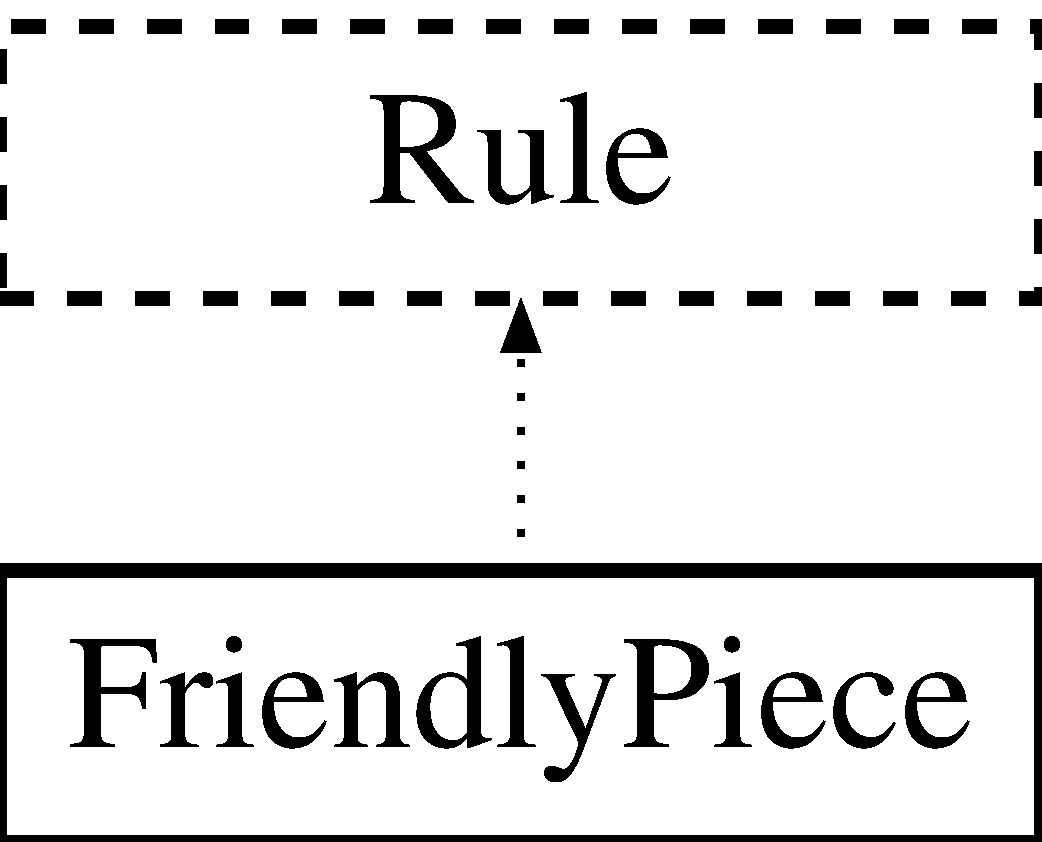
\includegraphics[height=2cm]{classFriendlyPiece}
\end{center}
\end{figure}
\subsection*{Public Member Functions}
\begin{DoxyCompactItemize}
\item 
\hyperlink{classFriendlyPiece_ac366bba74bf5c47475beb9da05875407}{FriendlyPiece} ()
\begin{DoxyCompactList}\small\item\em \hyperlink{classFriendlyPiece}{FriendlyPiece} creates a \hyperlink{classFriendlyPiece}{FriendlyPiece} object. \item\end{DoxyCompactList}\item 
int \hyperlink{classFriendlyPiece_aafce56ffcfb8c78a41529d482a89737d}{validMove} (vector$<$ vector$<$ \hyperlink{classPiece}{Piece} $\ast$ $>$ $>$ \&b, int ix, int iy, int dx, int dy)
\begin{DoxyCompactList}\small\item\em validMove checks if the there is a friendly piece in the place where your current piece wants to move. if valid calls \hyperlink{classKingInCheck}{KingInCheck}. if invalid return 0. \item\end{DoxyCompactList}\end{DoxyCompactItemize}


\subsection{Detailed Description}
\begin{DoxyAuthor}{Author}
Michael Wilson. 
\end{DoxyAuthor}
\begin{DoxyDate}{Date}
October 27,2014 
\end{DoxyDate}


\subsection{Constructor \& Destructor Documentation}
\hypertarget{classFriendlyPiece_ac366bba74bf5c47475beb9da05875407}{
\index{FriendlyPiece@{FriendlyPiece}!FriendlyPiece@{FriendlyPiece}}
\index{FriendlyPiece@{FriendlyPiece}!FriendlyPiece@{FriendlyPiece}}
\subsubsection[{FriendlyPiece}]{\setlength{\rightskip}{0pt plus 5cm}FriendlyPiece::FriendlyPiece ()}}
\label{classFriendlyPiece_ac366bba74bf5c47475beb9da05875407}


\hyperlink{classFriendlyPiece}{FriendlyPiece} creates a \hyperlink{classFriendlyPiece}{FriendlyPiece} object. 
\begin{DoxyParams}{Parameters}
\item[\mbox{$\leftarrow$} {\em b}]is a vector$<$ vector $<$ Piece$\ast$ $>$ $>$ object \item[\mbox{$\leftarrow$} {\em ix}]is the x for the initial location \item[\mbox{$\leftarrow$} {\em iy}]is the y for the initial location \item[\mbox{$\leftarrow$} {\em dx}]is the x for the destination location \item[\mbox{$\leftarrow$} {\em dy}]is the y for the destination location \end{DoxyParams}


\subsection{Member Function Documentation}
\hypertarget{classFriendlyPiece_aafce56ffcfb8c78a41529d482a89737d}{
\index{FriendlyPiece@{FriendlyPiece}!validMove@{validMove}}
\index{validMove@{validMove}!FriendlyPiece@{FriendlyPiece}}
\subsubsection[{validMove}]{\setlength{\rightskip}{0pt plus 5cm}int FriendlyPiece::validMove (vector$<$ vector$<$ {\bf Piece} $\ast$ $>$ $>$ \& {\em b}, \/  int {\em ix}, \/  int {\em iy}, \/  int {\em dx}, \/  int {\em dy})\hspace{0.3cm}{\ttfamily  \mbox{[}virtual\mbox{]}}}}
\label{classFriendlyPiece_aafce56ffcfb8c78a41529d482a89737d}


validMove checks if the there is a friendly piece in the place where your current piece wants to move. if valid calls \hyperlink{classKingInCheck}{KingInCheck}. if invalid return 0. \begin{DoxyReturn}{Returns}
an int 
\end{DoxyReturn}


Implements \hyperlink{classRule}{Rule}.

The documentation for this class was generated from the following files:\begin{DoxyCompactItemize}
\item 
source/Rules/\hyperlink{FriendlyPiece_8h}{FriendlyPiece.h}\item 
source/Rules/FriendlyPiece.cc\end{DoxyCompactItemize}

\hypertarget{classGame}{
\section{Game Class Reference}
\label{classGame}\index{Game@{Game}}
}
Inheritance diagram for Game::\begin{figure}[H]
\begin{center}
\leavevmode
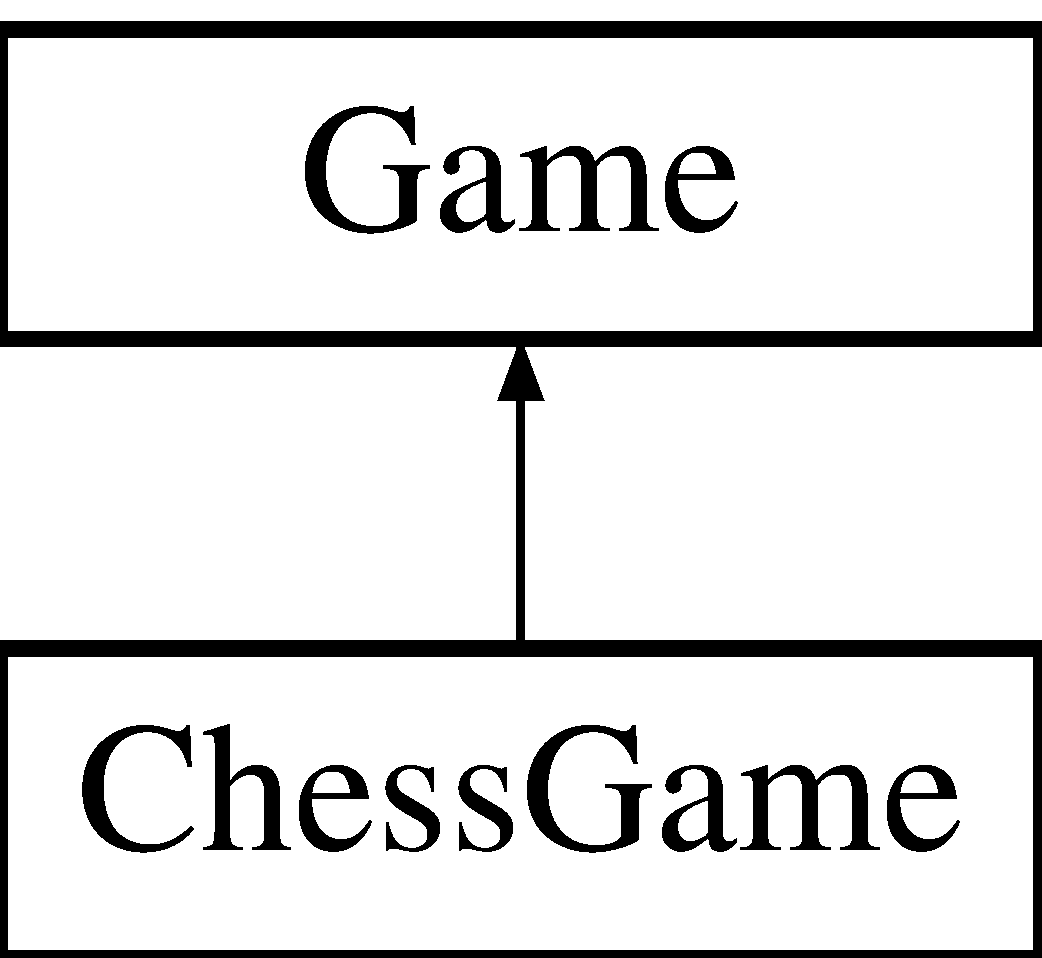
\includegraphics[height=2cm]{classGame}
\end{center}
\end{figure}
\subsection*{Public Member Functions}
\begin{DoxyCompactItemize}
\item 
\hyperlink{classGame_ad59df6562a58a614fda24622d3715b65}{Game} ()
\begin{DoxyCompactList}\small\item\em creates a \hyperlink{classGame}{Game} \item\end{DoxyCompactList}\item 
\hypertarget{classGame_ae3d112ca6e0e55150d2fdbc704474530}{
\hyperlink{classGame_ae3d112ca6e0e55150d2fdbc704474530}{$\sim$Game} ()}
\label{classGame_ae3d112ca6e0e55150d2fdbc704474530}

\begin{DoxyCompactList}\small\item\em \hyperlink{classGame}{Game} Destructor. \item\end{DoxyCompactList}\item 
\hyperlink{classBoard}{Board} $\ast$ \hyperlink{classGame_aac82d38c4540fcfaef89059865d1ce31}{getBoard} ()
\begin{DoxyCompactList}\small\item\em This function returns a pointer to board. \item\end{DoxyCompactList}\item 
void \hyperlink{classGame_af7023c9a15575e9ecd0ce68b7dfa0900}{setBoard} (\hyperlink{classBoard}{Board} b)
\begin{DoxyCompactList}\small\item\em sets board \item\end{DoxyCompactList}\item 
\hyperlink{classPlayer}{Player} $\ast$ \hyperlink{classGame_a01d7146d789990ee8195bdcca57c327e}{getPlayer1} ()
\begin{DoxyCompactList}\small\item\em This function returns a pointer to player1. \item\end{DoxyCompactList}\item 
void \hyperlink{classGame_a7d45a62dd687fcc5da92399ce4ce38e4}{setPlayer1} (\hyperlink{classPlayer}{Player} $\ast$p)
\begin{DoxyCompactList}\small\item\em sets player1 \item\end{DoxyCompactList}\item 
\hyperlink{classPlayer}{Player} $\ast$ \hyperlink{classGame_af0be7c35ebd72bbbf428331bd81aeacd}{getPlayer2} ()
\begin{DoxyCompactList}\small\item\em This function returns a pointer to player2. \item\end{DoxyCompactList}\item 
void \hyperlink{classGame_a4e8f17a058c9444a6257dc2e975b099f}{setPlayer2} (\hyperlink{classPlayer}{Player} $\ast$p)
\begin{DoxyCompactList}\small\item\em sets player2 \item\end{DoxyCompactList}\item 
void \hyperlink{classGame_a12f32ba70a35a0dcd1f527b4d4a0d2c4}{newGame} ()
\begin{DoxyCompactList}\small\item\em This function returns a pointer to chat. \item\end{DoxyCompactList}\item 
bool \hyperlink{classGame_ae8cc2b6b0b07924769189f2fa7e07e2d}{checkGameOver} ()
\begin{DoxyCompactList}\small\item\em This function returns whether the game is over or not. \item\end{DoxyCompactList}\item 
\hypertarget{classGame_a929c4b051000c20994aa75508f06e688}{
void \hyperlink{classGame_a929c4b051000c20994aa75508f06e688}{setGameOver} ()}
\label{classGame_a929c4b051000c20994aa75508f06e688}

\begin{DoxyCompactList}\small\item\em This function sets gameOver to true. \item\end{DoxyCompactList}\end{DoxyCompactItemize}


\subsection{Constructor \& Destructor Documentation}
\hypertarget{classGame_ad59df6562a58a614fda24622d3715b65}{
\index{Game@{Game}!Game@{Game}}
\index{Game@{Game}!Game@{Game}}
\subsubsection[{Game}]{\setlength{\rightskip}{0pt plus 5cm}Game::Game ()}}
\label{classGame_ad59df6562a58a614fda24622d3715b65}


creates a \hyperlink{classGame}{Game} Game.cc

\begin{DoxyAuthor}{Author}
Zackery Shortt 
\end{DoxyAuthor}
\begin{DoxyDate}{Date}
November 12, 2014 
\end{DoxyDate}


\subsection{Member Function Documentation}
\hypertarget{classGame_ae8cc2b6b0b07924769189f2fa7e07e2d}{
\index{Game@{Game}!checkGameOver@{checkGameOver}}
\index{checkGameOver@{checkGameOver}!Game@{Game}}
\subsubsection[{checkGameOver}]{\setlength{\rightskip}{0pt plus 5cm}bool Game::checkGameOver ()}}
\label{classGame_ae8cc2b6b0b07924769189f2fa7e07e2d}


This function returns whether the game is over or not. \begin{DoxyReturn}{Returns}
returns gameOver 
\end{DoxyReturn}
\hypertarget{classGame_aac82d38c4540fcfaef89059865d1ce31}{
\index{Game@{Game}!getBoard@{getBoard}}
\index{getBoard@{getBoard}!Game@{Game}}
\subsubsection[{getBoard}]{\setlength{\rightskip}{0pt plus 5cm}{\bf Board} $\ast$ Game::getBoard ()}}
\label{classGame_aac82d38c4540fcfaef89059865d1ce31}


This function returns a pointer to board. \begin{DoxyReturn}{Returns}
returns a pointer to board 
\end{DoxyReturn}
\hypertarget{classGame_a01d7146d789990ee8195bdcca57c327e}{
\index{Game@{Game}!getPlayer1@{getPlayer1}}
\index{getPlayer1@{getPlayer1}!Game@{Game}}
\subsubsection[{getPlayer1}]{\setlength{\rightskip}{0pt plus 5cm}{\bf Player} $\ast$ Game::getPlayer1 ()}}
\label{classGame_a01d7146d789990ee8195bdcca57c327e}


This function returns a pointer to player1. \begin{DoxyReturn}{Returns}
returns a pointer to player1 
\end{DoxyReturn}
\hypertarget{classGame_af0be7c35ebd72bbbf428331bd81aeacd}{
\index{Game@{Game}!getPlayer2@{getPlayer2}}
\index{getPlayer2@{getPlayer2}!Game@{Game}}
\subsubsection[{getPlayer2}]{\setlength{\rightskip}{0pt plus 5cm}{\bf Player} $\ast$ Game::getPlayer2 ()}}
\label{classGame_af0be7c35ebd72bbbf428331bd81aeacd}


This function returns a pointer to player2. \begin{DoxyReturn}{Returns}
returns a pointer to player2 
\end{DoxyReturn}
\hypertarget{classGame_a12f32ba70a35a0dcd1f527b4d4a0d2c4}{
\index{Game@{Game}!newGame@{newGame}}
\index{newGame@{newGame}!Game@{Game}}
\subsubsection[{newGame}]{\setlength{\rightskip}{0pt plus 5cm}void Game::newGame ()}}
\label{classGame_a12f32ba70a35a0dcd1f527b4d4a0d2c4}


This function returns a pointer to chat. \begin{DoxyReturn}{Returns}
returns a pointer to GameChat This function sets the board to newGame 
\end{DoxyReturn}
\hypertarget{classGame_af7023c9a15575e9ecd0ce68b7dfa0900}{
\index{Game@{Game}!setBoard@{setBoard}}
\index{setBoard@{setBoard}!Game@{Game}}
\subsubsection[{setBoard}]{\setlength{\rightskip}{0pt plus 5cm}void Game::setBoard ({\bf Board} {\em b})}}
\label{classGame_af7023c9a15575e9ecd0ce68b7dfa0900}


sets board 
\begin{DoxyParams}{Parameters}
\item[\mbox{$\leftarrow$} {\em This}]is the \hyperlink{classBoard}{Board} that \hyperlink{classGame}{Game} will be set to \end{DoxyParams}
\hypertarget{classGame_a7d45a62dd687fcc5da92399ce4ce38e4}{
\index{Game@{Game}!setPlayer1@{setPlayer1}}
\index{setPlayer1@{setPlayer1}!Game@{Game}}
\subsubsection[{setPlayer1}]{\setlength{\rightskip}{0pt plus 5cm}void Game::setPlayer1 ({\bf Player} $\ast$ {\em p})}}
\label{classGame_a7d45a62dd687fcc5da92399ce4ce38e4}


sets player1 
\begin{DoxyParams}{Parameters}
\item[\mbox{$\leftarrow$} {\em This}]is the player that player1 will be set to \end{DoxyParams}
\hypertarget{classGame_a4e8f17a058c9444a6257dc2e975b099f}{
\index{Game@{Game}!setPlayer2@{setPlayer2}}
\index{setPlayer2@{setPlayer2}!Game@{Game}}
\subsubsection[{setPlayer2}]{\setlength{\rightskip}{0pt plus 5cm}void Game::setPlayer2 ({\bf Player} $\ast$ {\em p})}}
\label{classGame_a4e8f17a058c9444a6257dc2e975b099f}


sets player2 
\begin{DoxyParams}{Parameters}
\item[\mbox{$\leftarrow$} {\em This}]is the player that player2 will be set to \end{DoxyParams}


The documentation for this class was generated from the following files:\begin{DoxyCompactItemize}
\item 
source/\hyperlink{Game_8h}{Game.h}\item 
source/Game.cc\end{DoxyCompactItemize}

\hypertarget{classGenericMenu}{
\section{GenericMenu Class Reference}
\label{classGenericMenu}\index{GenericMenu@{GenericMenu}}
}


\hyperlink{classGenericMenu}{GenericMenu} super class of all menus.  


{\ttfamily \#include $<$GenericMenu.h$>$}Inheritance diagram for GenericMenu::\begin{figure}[H]
\begin{center}
\leavevmode
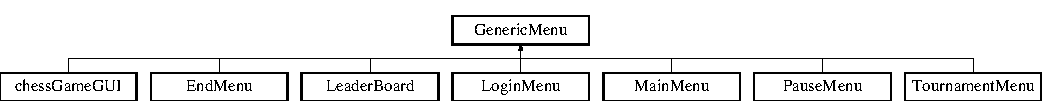
\includegraphics[height=1.35593cm]{classGenericMenu}
\end{center}
\end{figure}
\subsection*{Public Member Functions}
\begin{DoxyCompactItemize}
\item 
\hypertarget{classGenericMenu_ab0abde37b50eb17890bd223cc4807638}{
virtual \hyperlink{classGenericMenu_ab0abde37b50eb17890bd223cc4807638}{$\sim$GenericMenu} ()}
\label{classGenericMenu_ab0abde37b50eb17890bd223cc4807638}

\begin{DoxyCompactList}\small\item\em destructor put in place for the sake of posible further suclasses needing adestructor. \item\end{DoxyCompactList}\item 
virtual \hyperlink{classGenericMenu}{GenericMenu} $\ast$ \hyperlink{classGenericMenu_a290ad7ec3331edc968190b1d7b48a397}{menufunc} (string \&opt, \hyperlink{classstatus}{status} $\ast$\&info)=0
\begin{DoxyCompactList}\small\item\em menufunc is the general handler for implementing the functionality of this menu class \item\end{DoxyCompactList}\end{DoxyCompactItemize}


\subsection{Detailed Description}
\hyperlink{classGenericMenu}{GenericMenu} super class of all menus. 

\subsection{Member Function Documentation}
\hypertarget{classGenericMenu_a290ad7ec3331edc968190b1d7b48a397}{
\index{GenericMenu@{GenericMenu}!menufunc@{menufunc}}
\index{menufunc@{menufunc}!GenericMenu@{GenericMenu}}
\subsubsection[{menufunc}]{\setlength{\rightskip}{0pt plus 5cm}virtual {\bf GenericMenu}$\ast$ GenericMenu::menufunc (string \& {\em opt}, \/  {\bf status} $\ast$\& {\em info})\hspace{0.3cm}{\ttfamily  \mbox{[}pure virtual\mbox{]}}}}
\label{classGenericMenu_a290ad7ec3331edc968190b1d7b48a397}


menufunc is the general handler for implementing the functionality of this menu class 
\begin{DoxyParams}{Parameters}
\item[\mbox{$\leftarrow$} {\em opt}]a reference for the program to decide where it must go in the main param\mbox{[}in\mbox{]} \hyperlink{classstatus}{status} is a class to enable manipulation of the current game and players between classes \end{DoxyParams}


Implemented in \hyperlink{classchessGameGUI_afcafe4d3b432bae7cd8439b689886a8d}{chessGameGUI}, \hyperlink{classEndMenu_a8fc10a35897496066f1db862bad44028}{EndMenu}, \hyperlink{classLeaderBoard_a848e37073627647d9ace936690d6e3bb}{LeaderBoard}, \hyperlink{classLoginMenu_a2f391af29531a557e0547294e97132fe}{LoginMenu}, \hyperlink{classMainMenu_aed53ec0c027843a2a1204235fe2924ea}{MainMenu}, \hyperlink{classPauseMenu_a7926ffe9dd0aa74281d8cb8126cd9c10}{PauseMenu}, and \hyperlink{classTournamentMenu_a86ce030ba6728404ddc49aaacb45dd34}{TournamentMenu}.

The documentation for this class was generated from the following file:\begin{DoxyCompactItemize}
\item 
source/Menu/\hyperlink{GenericMenu_8h}{GenericMenu.h}\end{DoxyCompactItemize}

\hypertarget{classKingInCheck}{
\section{KingInCheck Class Reference}
\label{classKingInCheck}\index{KingInCheck@{KingInCheck}}
}
Inheritance diagram for KingInCheck::\begin{figure}[H]
\begin{center}
\leavevmode
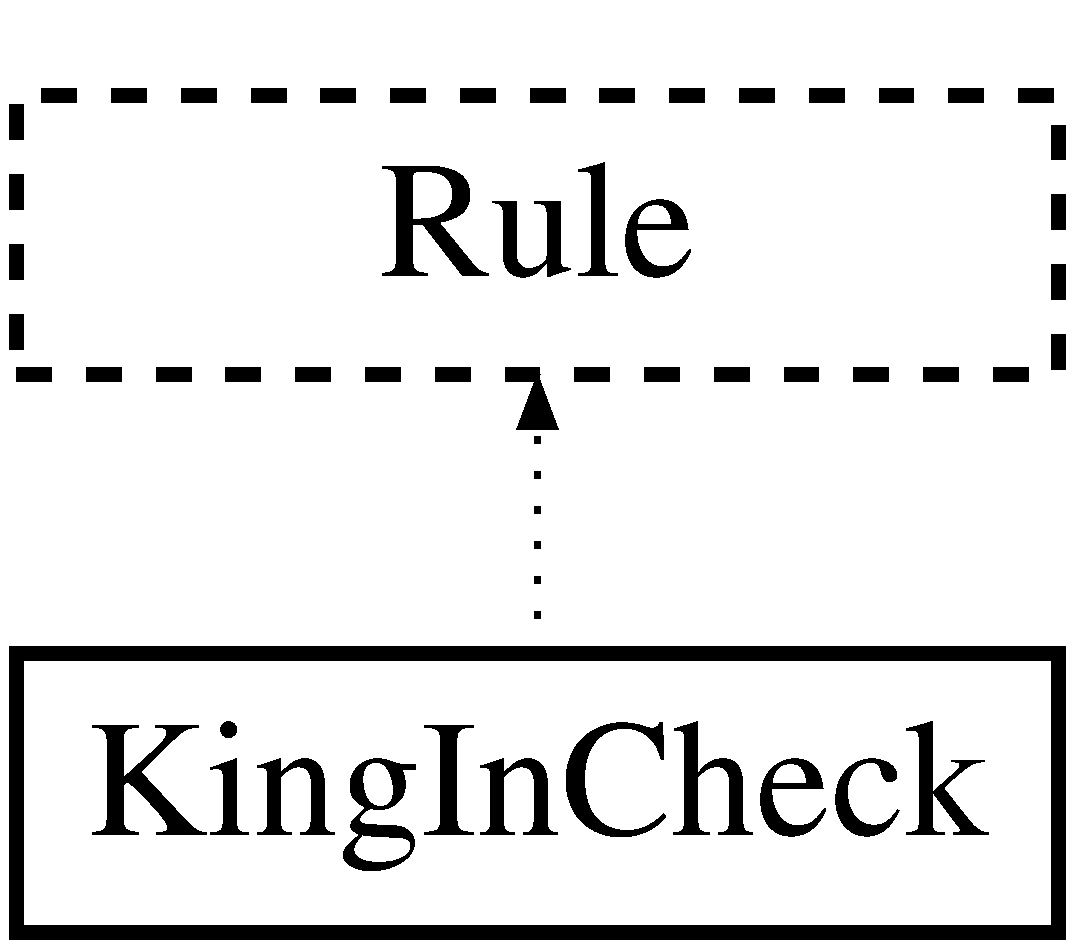
\includegraphics[height=2cm]{classKingInCheck}
\end{center}
\end{figure}
\subsection*{Public Member Functions}
\begin{DoxyCompactItemize}
\item 
\hyperlink{classKingInCheck_ac3c04d5e0646f84c185e61ef739262ee}{KingInCheck} ()
\begin{DoxyCompactList}\small\item\em \hyperlink{classKingInCheck}{KingInCheck} creates a \hyperlink{classKingInCheck}{KingInCheck} object. \item\end{DoxyCompactList}\item 
int \hyperlink{classKingInCheck_a5c9860dc659beddf2c8e7e471778c60c}{validMove} (vector$<$ vector$<$ \hyperlink{classPiece}{Piece} $\ast$ $>$ $>$ \&b, int ix, int iy, int dx, int dy)
\begin{DoxyCompactList}\small\item\em validMove checks if the king is in check. if valid call CheckTure. if invalid return 0. \item\end{DoxyCompactList}\item 
\hypertarget{classKingInCheck_a487117dfeb79f8d4f9c62ce02f9251ce}{
bool {\bfseries CheckMate} (vector$<$ vector$<$ \hyperlink{classPiece}{Piece} $\ast$ $>$ $>$ \&b, int x, int y)}
\label{classKingInCheck_a487117dfeb79f8d4f9c62ce02f9251ce}

\end{DoxyCompactItemize}


\subsection{Constructor \& Destructor Documentation}
\hypertarget{classKingInCheck_ac3c04d5e0646f84c185e61ef739262ee}{
\index{KingInCheck@{KingInCheck}!KingInCheck@{KingInCheck}}
\index{KingInCheck@{KingInCheck}!KingInCheck@{KingInCheck}}
\subsubsection[{KingInCheck}]{\setlength{\rightskip}{0pt plus 5cm}KingInCheck::KingInCheck ()}}
\label{classKingInCheck_ac3c04d5e0646f84c185e61ef739262ee}


\hyperlink{classKingInCheck}{KingInCheck} creates a \hyperlink{classKingInCheck}{KingInCheck} object. 
\begin{DoxyParams}{Parameters}
\item[\mbox{$\leftarrow$} {\em b}]is a vector$<$ vector $<$ Piece$\ast$ $>$ $>$ object \item[\mbox{$\leftarrow$} {\em ix}]is the x for the initial location \item[\mbox{$\leftarrow$} {\em iy}]is the y for the initial location \item[\mbox{$\leftarrow$} {\em dx}]is the x for the destination location \item[\mbox{$\leftarrow$} {\em dy}]is the y for the destination location \end{DoxyParams}


\subsection{Member Function Documentation}
\hypertarget{classKingInCheck_a5c9860dc659beddf2c8e7e471778c60c}{
\index{KingInCheck@{KingInCheck}!validMove@{validMove}}
\index{validMove@{validMove}!KingInCheck@{KingInCheck}}
\subsubsection[{validMove}]{\setlength{\rightskip}{0pt plus 5cm}int KingInCheck::validMove (vector$<$ vector$<$ {\bf Piece} $\ast$ $>$ $>$ \& {\em b}, \/  int {\em ix}, \/  int {\em iy}, \/  int {\em dx}, \/  int {\em dy})\hspace{0.3cm}{\ttfamily  \mbox{[}virtual\mbox{]}}}}
\label{classKingInCheck_a5c9860dc659beddf2c8e7e471778c60c}


validMove checks if the king is in check. if valid call CheckTure. if invalid return 0. \begin{DoxyReturn}{Returns}
an int 
\end{DoxyReturn}


Checks if the king is still on the board if it is not this will result in an end of game 

Implements \hyperlink{classRule}{Rule}.

The documentation for this class was generated from the following files:\begin{DoxyCompactItemize}
\item 
source/Rules/\hyperlink{KingInCheck_8h}{KingInCheck.h}\item 
source/Rules/KingInCheck.cc\end{DoxyCompactItemize}

\hypertarget{classKingMove}{
\section{KingMove Class Reference}
\label{classKingMove}\index{KingMove@{KingMove}}
}
Inheritance diagram for KingMove::\begin{figure}[H]
\begin{center}
\leavevmode
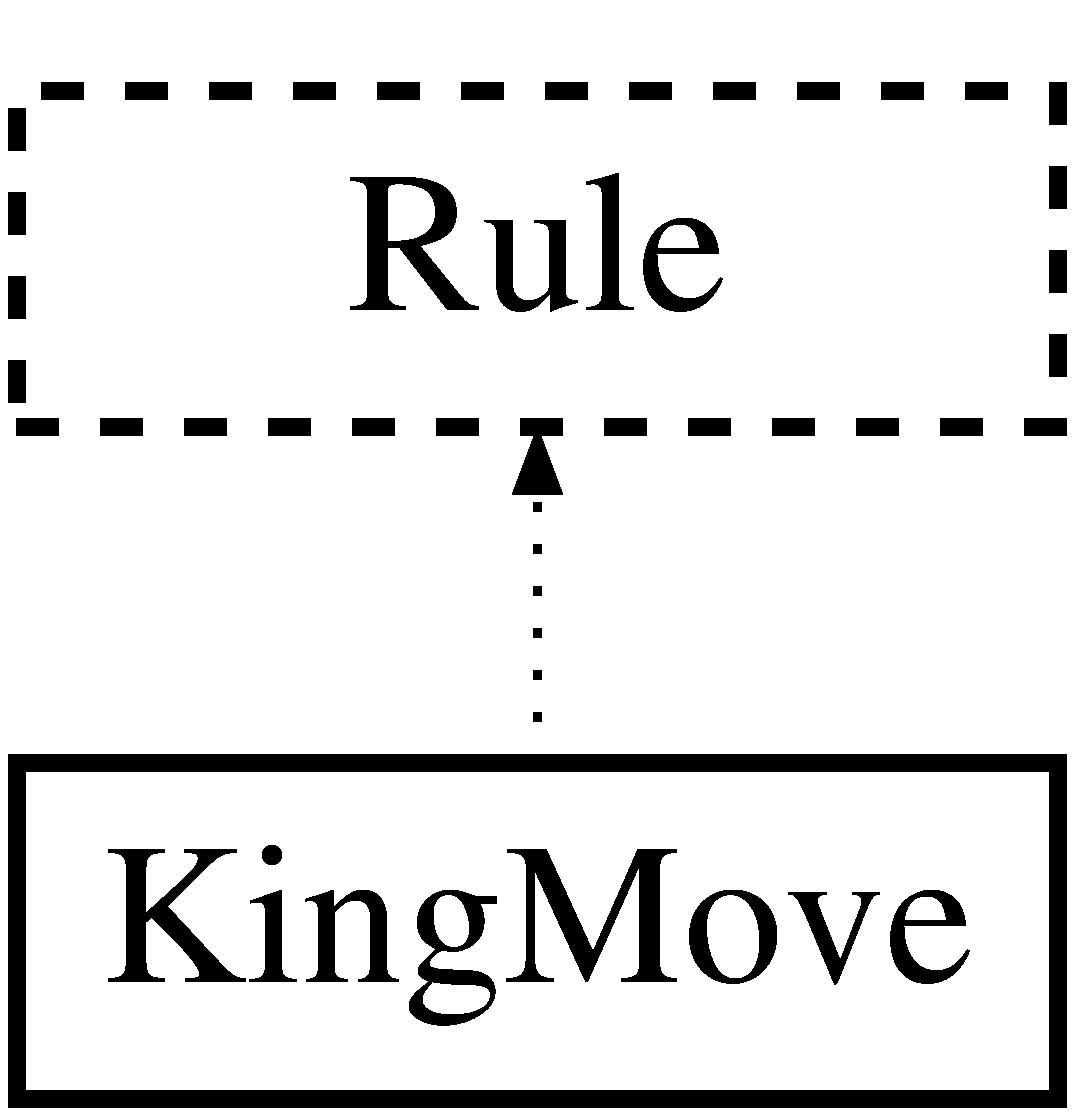
\includegraphics[height=2cm]{classKingMove}
\end{center}
\end{figure}
\subsection*{Public Member Functions}
\begin{DoxyCompactItemize}
\item 
\hyperlink{classKingMove_a6ab2c891e1498dead1e1d7df7e4a9924}{KingMove} ()
\begin{DoxyCompactList}\small\item\em \hyperlink{classKingMove}{KingMove} creates a \hyperlink{classKingMove}{KingMove} object. \item\end{DoxyCompactList}\item 
int \hyperlink{classKingMove_a2c3086623fc47b43cef95ba6ee95915b}{validMove} (vector$<$ vector$<$ \hyperlink{classPiece}{Piece} $\ast$ $>$ $>$ \&b, int ix, int iy, int dx, int dy)
\begin{DoxyCompactList}\small\item\em validMove checks if the pieces left alive are the bishop and king or the knight and king it will return 2 else return 1. \item\end{DoxyCompactList}\end{DoxyCompactItemize}


\subsection{Constructor \& Destructor Documentation}
\hypertarget{classKingMove_a6ab2c891e1498dead1e1d7df7e4a9924}{
\index{KingMove@{KingMove}!KingMove@{KingMove}}
\index{KingMove@{KingMove}!KingMove@{KingMove}}
\subsubsection[{KingMove}]{\setlength{\rightskip}{0pt plus 5cm}KingMove::KingMove ()}}
\label{classKingMove_a6ab2c891e1498dead1e1d7df7e4a9924}


\hyperlink{classKingMove}{KingMove} creates a \hyperlink{classKingMove}{KingMove} object. 
\begin{DoxyParams}{Parameters}
\item[\mbox{$\leftarrow$} {\em b}]is a vector$<$ vector $<$ Piece$\ast$ $>$ $>$ object \item[\mbox{$\leftarrow$} {\em ix}]is the x for the initial location \item[\mbox{$\leftarrow$} {\em iy}]is the y for the initial location \item[\mbox{$\leftarrow$} {\em dx}]is the x for the destination location \item[\mbox{$\leftarrow$} {\em dy}]is the y for the destination location \end{DoxyParams}


\subsection{Member Function Documentation}
\hypertarget{classKingMove_a2c3086623fc47b43cef95ba6ee95915b}{
\index{KingMove@{KingMove}!validMove@{validMove}}
\index{validMove@{validMove}!KingMove@{KingMove}}
\subsubsection[{validMove}]{\setlength{\rightskip}{0pt plus 5cm}int KingMove::validMove (vector$<$ vector$<$ {\bf Piece} $\ast$ $>$ $>$ \& {\em b}, \/  int {\em ix}, \/  int {\em iy}, \/  int {\em dx}, \/  int {\em dy})\hspace{0.3cm}{\ttfamily  \mbox{[}virtual\mbox{]}}}}
\label{classKingMove_a2c3086623fc47b43cef95ba6ee95915b}


validMove checks if the pieces left alive are the bishop and king or the knight and king it will return 2 else return 1. \begin{DoxyReturn}{Returns}
an int 
\end{DoxyReturn}


Implements \hyperlink{classRule}{Rule}.

The documentation for this class was generated from the following files:\begin{DoxyCompactItemize}
\item 
source/Rules/\hyperlink{KingMove_8h}{KingMove.h}\item 
source/Rules/KingMove.cc\end{DoxyCompactItemize}

\hypertarget{classKingPiece}{
\section{KingPiece Class Reference}
\label{classKingPiece}\index{KingPiece@{KingPiece}}
}


a class for all King Piece`s.  


{\ttfamily \#include $<$KingPiece.h$>$}Inheritance diagram for KingPiece::\begin{figure}[H]
\begin{center}
\leavevmode
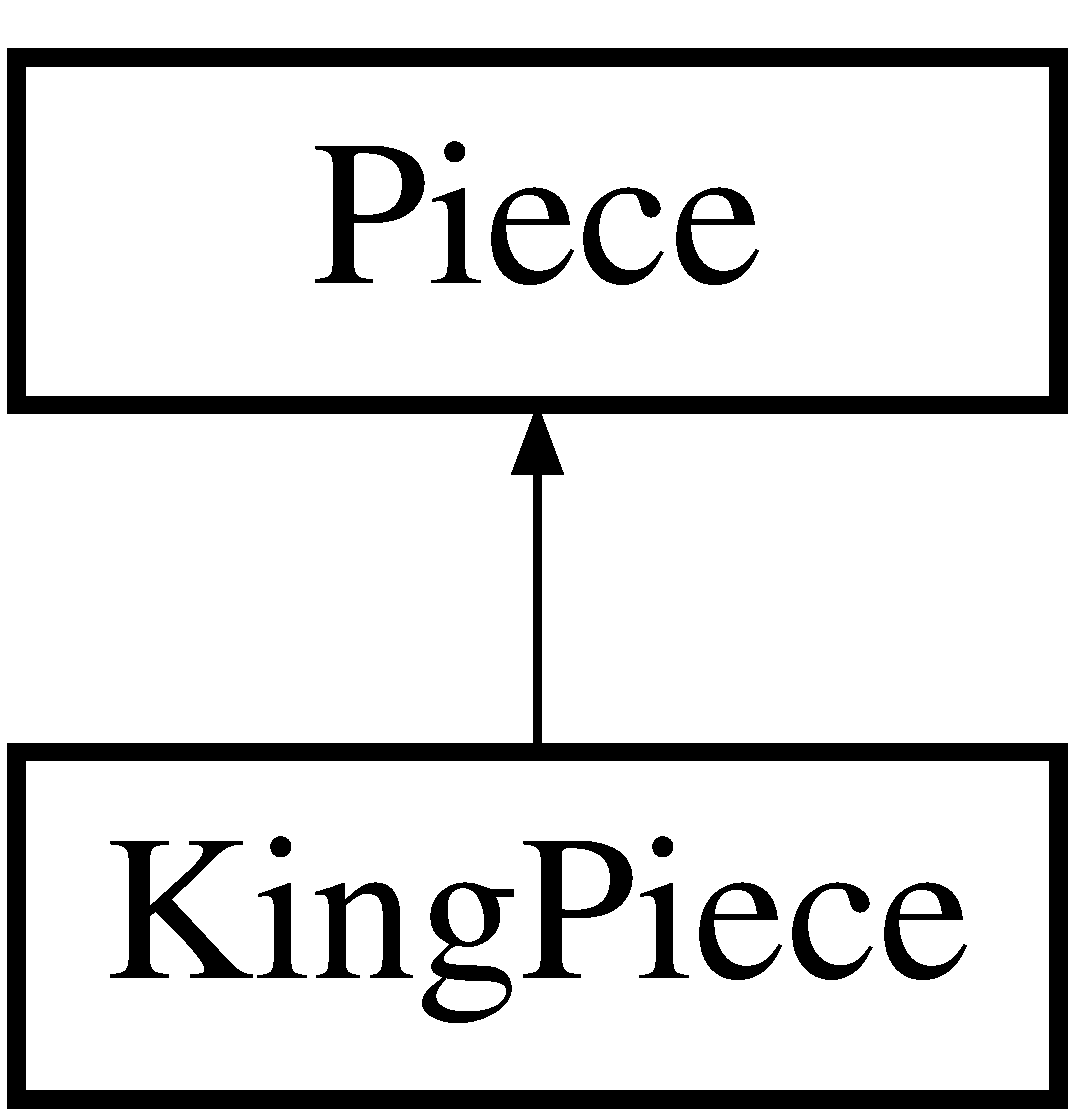
\includegraphics[height=2cm]{classKingPiece}
\end{center}
\end{figure}
\subsection*{Public Member Functions}
\begin{DoxyCompactItemize}
\item 
\hypertarget{classKingPiece_a9851298aebec5797b2497c9c3a8397f9}{
\hyperlink{classKingPiece_a9851298aebec5797b2497c9c3a8397f9}{KingPiece} (int c=0)}
\label{classKingPiece_a9851298aebec5797b2497c9c3a8397f9}

\begin{DoxyCompactList}\small\item\em creates a \hyperlink{classPiece}{Piece} object \item\end{DoxyCompactList}\item 
int \hyperlink{classKingPiece_ac15e38c6ceaccae6879ec70211c2ab28}{getColor} () const 
\begin{DoxyCompactList}\small\item\em gets the color of the King \hyperlink{classPiece}{Piece} \item\end{DoxyCompactList}\item 
void \hyperlink{classKingPiece_ab7a9023dda46c21a566675623f1b4a32}{setColor} (int colorOfPiece)
\begin{DoxyCompactList}\small\item\em sets the Color of the King \hyperlink{classPiece}{Piece} \item\end{DoxyCompactList}\item 
string \hyperlink{classKingPiece_ac93de53a7adee6e5ad33284f0fd6aa2e}{getType} () const 
\begin{DoxyCompactList}\small\item\em Returns King to user. \item\end{DoxyCompactList}\item 
int \hyperlink{classKingPiece_ae2ae8557d6d6e5fd1dcacdf7839de49f}{validMove} (vector$<$ vector$<$ \hyperlink{classPiece}{Piece} $\ast$ $>$ $>$ gameBoard, int ix, int iy, int dx, int dy)
\begin{DoxyCompactList}\small\item\em validates a move based on the King rules. \item\end{DoxyCompactList}\end{DoxyCompactItemize}


\subsection{Detailed Description}
a class for all King Piece`s. 

\subsection{Member Function Documentation}
\hypertarget{classKingPiece_ac15e38c6ceaccae6879ec70211c2ab28}{
\index{KingPiece@{KingPiece}!getColor@{getColor}}
\index{getColor@{getColor}!KingPiece@{KingPiece}}
\subsubsection[{getColor}]{\setlength{\rightskip}{0pt plus 5cm}int KingPiece::getColor () const\hspace{0.3cm}{\ttfamily  \mbox{[}virtual\mbox{]}}}}
\label{classKingPiece_ac15e38c6ceaccae6879ec70211c2ab28}


gets the color of the King \hyperlink{classPiece}{Piece} \begin{DoxyReturn}{Returns}
int a 0 if white and 1 if black 
\end{DoxyReturn}


Implements \hyperlink{classPiece_a1376072d4815719e60253ce5688df95c}{Piece}.\hypertarget{classKingPiece_ac93de53a7adee6e5ad33284f0fd6aa2e}{
\index{KingPiece@{KingPiece}!getType@{getType}}
\index{getType@{getType}!KingPiece@{KingPiece}}
\subsubsection[{getType}]{\setlength{\rightskip}{0pt plus 5cm}string KingPiece::getType () const\hspace{0.3cm}{\ttfamily  \mbox{[}virtual\mbox{]}}}}
\label{classKingPiece_ac93de53a7adee6e5ad33284f0fd6aa2e}


Returns King to user. \begin{DoxyReturn}{Returns}
a string that will return King. 
\end{DoxyReturn}


Implements \hyperlink{classPiece_a5b88fcd786bb30b345b24fbc3ab24ab9}{Piece}.\hypertarget{classKingPiece_ab7a9023dda46c21a566675623f1b4a32}{
\index{KingPiece@{KingPiece}!setColor@{setColor}}
\index{setColor@{setColor}!KingPiece@{KingPiece}}
\subsubsection[{setColor}]{\setlength{\rightskip}{0pt plus 5cm}void KingPiece::setColor (int {\em colorOfPiece})\hspace{0.3cm}{\ttfamily  \mbox{[}virtual\mbox{]}}}}
\label{classKingPiece_ab7a9023dda46c21a566675623f1b4a32}


sets the Color of the King \hyperlink{classPiece}{Piece} 
\begin{DoxyParams}{Parameters}
\item[\mbox{$\leftarrow$} {\em colorOfPiece}]sets the King Piece`s color \end{DoxyParams}


Implements \hyperlink{classPiece_a1387cb503dca308ac1e3bbe38a70a073}{Piece}.\hypertarget{classKingPiece_ae2ae8557d6d6e5fd1dcacdf7839de49f}{
\index{KingPiece@{KingPiece}!validMove@{validMove}}
\index{validMove@{validMove}!KingPiece@{KingPiece}}
\subsubsection[{validMove}]{\setlength{\rightskip}{0pt plus 5cm}int KingPiece::validMove (vector$<$ vector$<$ {\bf Piece} $\ast$ $>$ $>$ {\em gameBoard}, \/  int {\em ix}, \/  int {\em iy}, \/  int {\em dx}, \/  int {\em dy})}}
\label{classKingPiece_ae2ae8557d6d6e5fd1dcacdf7839de49f}


validates a move based on the King rules. 
\begin{DoxyParams}{Parameters}
\item[\mbox{$\leftarrow$} {\em board}]A \hyperlink{classBoard}{Board} that will contain the currect board state \item[\mbox{$\leftarrow$} {\em ix}]A int that holds the x coordinate of where the piece is moving from \item[\mbox{$\leftarrow$} {\em iy}]A int that holds the y coordinate of where the piece is moving from \item[\mbox{$\leftarrow$} {\em dx}]A int that holds the x coordinate of where the piece is moving to \item[\mbox{$\leftarrow$} {\em dy}]A int that holds the y coordinate of where the piece is moving to \end{DoxyParams}


The documentation for this class was generated from the following files:\begin{DoxyCompactItemize}
\item 
source/Piece/\hyperlink{KingPiece_8h}{KingPiece.h}\item 
source/Piece/KingPiece.cc\end{DoxyCompactItemize}

\hypertarget{classKnightMove}{
\section{KnightMove Class Reference}
\label{classKnightMove}\index{KnightMove@{KnightMove}}
}
Inheritance diagram for KnightMove::\begin{figure}[H]
\begin{center}
\leavevmode
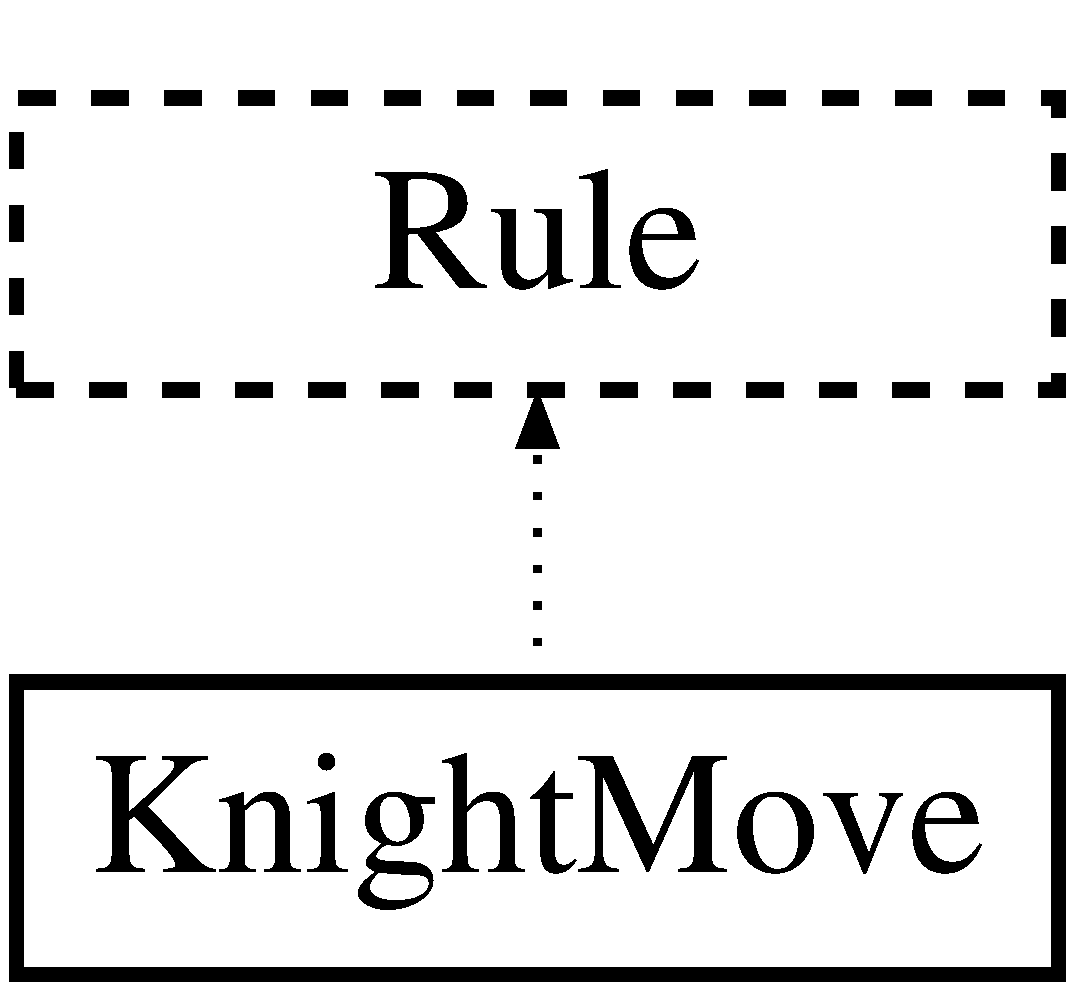
\includegraphics[height=2cm]{classKnightMove}
\end{center}
\end{figure}
\subsection*{Public Member Functions}
\begin{DoxyCompactItemize}
\item 
\hyperlink{classKnightMove_af312e58dbda8f4c6e241d70cf24f6b1a}{KnightMove} ()
\begin{DoxyCompactList}\small\item\em \hyperlink{classKnightMove}{KnightMove} creates a \hyperlink{classKnightMove}{KnightMove} object. \item\end{DoxyCompactList}\item 
int \hyperlink{classKnightMove_a0bf2d52e9202f4662d7920321bd0c81a}{validMove} (vector$<$ vector$<$ \hyperlink{classPiece}{Piece} $\ast$ $>$ $>$ \&b, int ix, int iy, int dx, int dy)
\begin{DoxyCompactList}\small\item\em validMove if the knights requested location id ((y+2 or y -\/ 2) and (x+1 or x -\/1)) or (( y+1 or y -\/1) and (x + 2 or x -\/2)) then go to \hyperlink{classFriendlyPiece}{FriendlyPiece} rule else return 0. \item\end{DoxyCompactList}\end{DoxyCompactItemize}


\subsection{Constructor \& Destructor Documentation}
\hypertarget{classKnightMove_af312e58dbda8f4c6e241d70cf24f6b1a}{
\index{KnightMove@{KnightMove}!KnightMove@{KnightMove}}
\index{KnightMove@{KnightMove}!KnightMove@{KnightMove}}
\subsubsection[{KnightMove}]{\setlength{\rightskip}{0pt plus 5cm}KnightMove::KnightMove ()}}
\label{classKnightMove_af312e58dbda8f4c6e241d70cf24f6b1a}


\hyperlink{classKnightMove}{KnightMove} creates a \hyperlink{classKnightMove}{KnightMove} object. 
\begin{DoxyParams}{Parameters}
\item[\mbox{$\leftarrow$} {\em b}]is a vector$<$ vector $<$ Piece$\ast$ $>$ $>$ object \item[\mbox{$\leftarrow$} {\em ix}]is the x for the initial location \item[\mbox{$\leftarrow$} {\em iy}]is the y for the initial location \item[\mbox{$\leftarrow$} {\em dx}]is the x for the destination location \item[\mbox{$\leftarrow$} {\em dy}]is the y for the destination location \end{DoxyParams}


\subsection{Member Function Documentation}
\hypertarget{classKnightMove_a0bf2d52e9202f4662d7920321bd0c81a}{
\index{KnightMove@{KnightMove}!validMove@{validMove}}
\index{validMove@{validMove}!KnightMove@{KnightMove}}
\subsubsection[{validMove}]{\setlength{\rightskip}{0pt plus 5cm}int KnightMove::validMove (vector$<$ vector$<$ {\bf Piece} $\ast$ $>$ $>$ \& {\em b}, \/  int {\em ix}, \/  int {\em iy}, \/  int {\em dx}, \/  int {\em dy})\hspace{0.3cm}{\ttfamily  \mbox{[}virtual\mbox{]}}}}
\label{classKnightMove_a0bf2d52e9202f4662d7920321bd0c81a}


validMove if the knights requested location id ((y+2 or y -\/ 2) and (x+1 or x -\/1)) or (( y+1 or y -\/1) and (x + 2 or x -\/2)) then go to \hyperlink{classFriendlyPiece}{FriendlyPiece} rule else return 0. \begin{DoxyReturn}{Returns}
an int 
\end{DoxyReturn}


Implements \hyperlink{classRule}{Rule}.

The documentation for this class was generated from the following files:\begin{DoxyCompactItemize}
\item 
source/Rules/\hyperlink{KnightMove_8h}{KnightMove.h}\item 
source/Rules/KnightMove.cc\end{DoxyCompactItemize}

\hypertarget{classKnightPiece}{
\section{KnightPiece Class Reference}
\label{classKnightPiece}\index{KnightPiece@{KnightPiece}}
}


a class for all Knight Piece`s.  


{\ttfamily \#include $<$KnightPiece.h$>$}Inheritance diagram for KnightPiece::\begin{figure}[H]
\begin{center}
\leavevmode
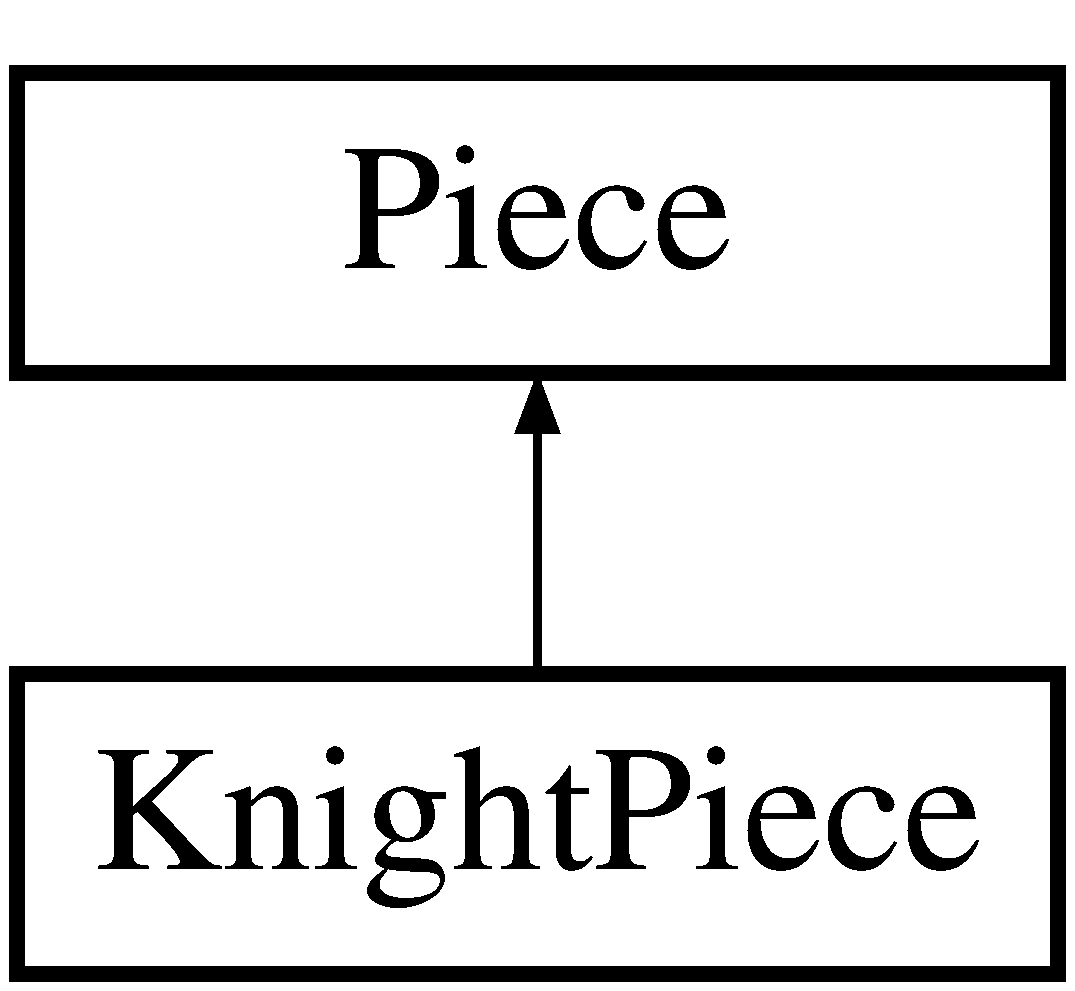
\includegraphics[height=2cm]{classKnightPiece}
\end{center}
\end{figure}
\subsection*{Public Member Functions}
\begin{DoxyCompactItemize}
\item 
\hypertarget{classKnightPiece_a3575ffe197fb0b40c6c7791d36fd2418}{
\hyperlink{classKnightPiece_a3575ffe197fb0b40c6c7791d36fd2418}{KnightPiece} (int c=0)}
\label{classKnightPiece_a3575ffe197fb0b40c6c7791d36fd2418}

\begin{DoxyCompactList}\small\item\em creates a \hyperlink{classPiece}{Piece} object \item\end{DoxyCompactList}\item 
int \hyperlink{classKnightPiece_ab8ef95a1a625e461ada96e4692599770}{getColor} () const 
\begin{DoxyCompactList}\small\item\em gets the color of the Knight \hyperlink{classPiece}{Piece} \item\end{DoxyCompactList}\item 
void \hyperlink{classKnightPiece_a928091c9100f4e3bc2bb2d10535ccc49}{setColor} (int colorOfPiece)
\begin{DoxyCompactList}\small\item\em sets the Color of the Knight \hyperlink{classPiece}{Piece} \item\end{DoxyCompactList}\item 
string \hyperlink{classKnightPiece_a3b141e4014d09bba70625ccb2129efcc}{getType} () const 
\begin{DoxyCompactList}\small\item\em Returns Knight to user. \item\end{DoxyCompactList}\item 
int \hyperlink{classKnightPiece_a9c8f78a9ef9a5e26c8011cb37a16e702}{validMove} (vector$<$ vector$<$ \hyperlink{classPiece}{Piece} $\ast$ $>$ $>$ gameBoard, int ix, int iy, int dx, int dy)
\begin{DoxyCompactList}\small\item\em validates a move based on the Knight rules. \item\end{DoxyCompactList}\end{DoxyCompactItemize}


\subsection{Detailed Description}
a class for all Knight Piece`s. 

\subsection{Member Function Documentation}
\hypertarget{classKnightPiece_ab8ef95a1a625e461ada96e4692599770}{
\index{KnightPiece@{KnightPiece}!getColor@{getColor}}
\index{getColor@{getColor}!KnightPiece@{KnightPiece}}
\subsubsection[{getColor}]{\setlength{\rightskip}{0pt plus 5cm}int KnightPiece::getColor () const\hspace{0.3cm}{\ttfamily  \mbox{[}virtual\mbox{]}}}}
\label{classKnightPiece_ab8ef95a1a625e461ada96e4692599770}


gets the color of the Knight \hyperlink{classPiece}{Piece} \begin{DoxyReturn}{Returns}
int a 0 if white and 1 if black 
\end{DoxyReturn}


Implements \hyperlink{classPiece_a1376072d4815719e60253ce5688df95c}{Piece}.\hypertarget{classKnightPiece_a3b141e4014d09bba70625ccb2129efcc}{
\index{KnightPiece@{KnightPiece}!getType@{getType}}
\index{getType@{getType}!KnightPiece@{KnightPiece}}
\subsubsection[{getType}]{\setlength{\rightskip}{0pt plus 5cm}string KnightPiece::getType () const\hspace{0.3cm}{\ttfamily  \mbox{[}virtual\mbox{]}}}}
\label{classKnightPiece_a3b141e4014d09bba70625ccb2129efcc}


Returns Knight to user. \begin{DoxyReturn}{Returns}
a string that will return Knight Type. 
\end{DoxyReturn}


Implements \hyperlink{classPiece_a5b88fcd786bb30b345b24fbc3ab24ab9}{Piece}.\hypertarget{classKnightPiece_a928091c9100f4e3bc2bb2d10535ccc49}{
\index{KnightPiece@{KnightPiece}!setColor@{setColor}}
\index{setColor@{setColor}!KnightPiece@{KnightPiece}}
\subsubsection[{setColor}]{\setlength{\rightskip}{0pt plus 5cm}void KnightPiece::setColor (int {\em colorOfPiece})\hspace{0.3cm}{\ttfamily  \mbox{[}virtual\mbox{]}}}}
\label{classKnightPiece_a928091c9100f4e3bc2bb2d10535ccc49}


sets the Color of the Knight \hyperlink{classPiece}{Piece} 
\begin{DoxyParams}{Parameters}
\item[\mbox{$\leftarrow$} {\em colorOfPiece}]sets the Pawn Piece`s color \end{DoxyParams}


Implements \hyperlink{classPiece_a1387cb503dca308ac1e3bbe38a70a073}{Piece}.\hypertarget{classKnightPiece_a9c8f78a9ef9a5e26c8011cb37a16e702}{
\index{KnightPiece@{KnightPiece}!validMove@{validMove}}
\index{validMove@{validMove}!KnightPiece@{KnightPiece}}
\subsubsection[{validMove}]{\setlength{\rightskip}{0pt plus 5cm}int KnightPiece::validMove (vector$<$ vector$<$ {\bf Piece} $\ast$ $>$ $>$ {\em gameBoard}, \/  int {\em ix}, \/  int {\em iy}, \/  int {\em dx}, \/  int {\em dy})}}
\label{classKnightPiece_a9c8f78a9ef9a5e26c8011cb37a16e702}


validates a move based on the Knight rules. 
\begin{DoxyParams}{Parameters}
\item[\mbox{$\leftarrow$} {\em board}]A \hyperlink{classBoard}{Board} that will contain the currect board state \item[\mbox{$\leftarrow$} {\em ix}]A int that holds the x coordinate of where the piece is moving from \item[\mbox{$\leftarrow$} {\em iy}]A int that holds the y coordinate of where the piece is moving from \item[\mbox{$\leftarrow$} {\em dx}]A int that holds the x coordinate of where the piece is moving to \item[\mbox{$\leftarrow$} {\em dy}]A int that holds the y coordinate of where the piece is moving to \end{DoxyParams}


The documentation for this class was generated from the following files:\begin{DoxyCompactItemize}
\item 
source/Piece/\hyperlink{KnightPiece_8h}{KnightPiece.h}\item 
source/Piece/KnightPiece.cc\end{DoxyCompactItemize}

\hypertarget{classLeaderBoard}{
\section{LeaderBoard Class Reference}
\label{classLeaderBoard}\index{LeaderBoard@{LeaderBoard}}
}
Inheritance diagram for LeaderBoard::\begin{figure}[H]
\begin{center}
\leavevmode
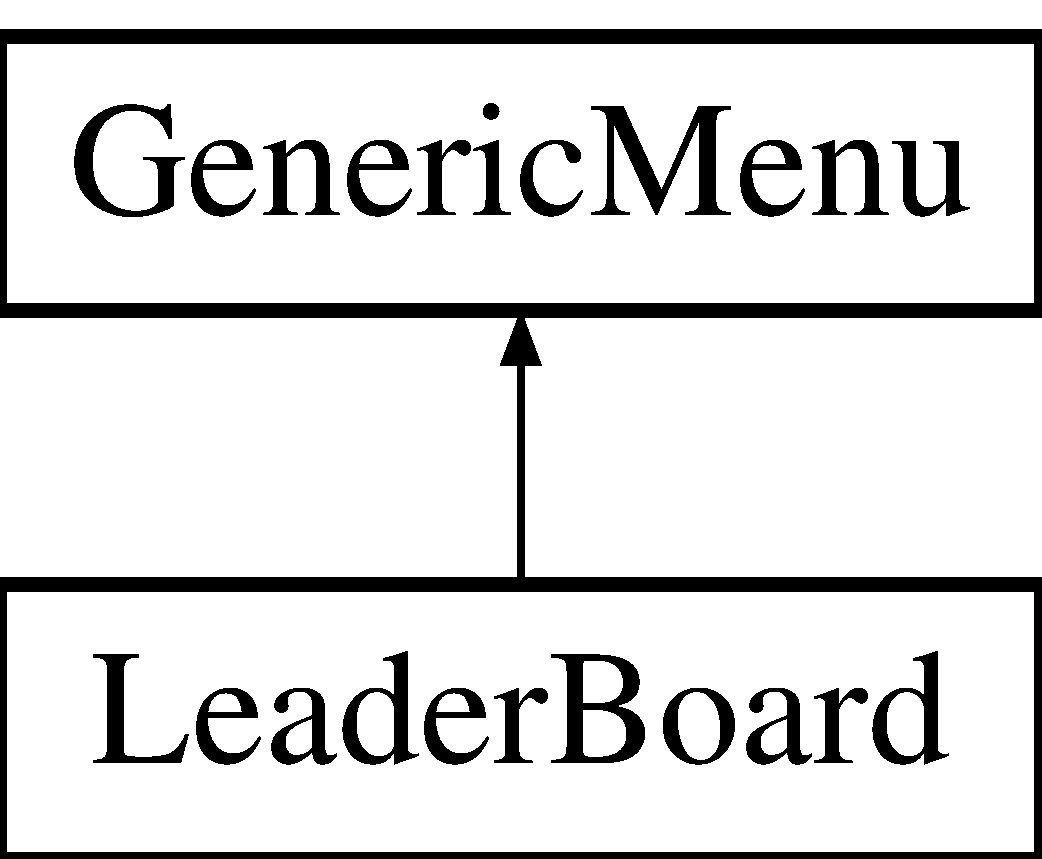
\includegraphics[height=2cm]{classLeaderBoard}
\end{center}
\end{figure}
\subsection*{Public Member Functions}
\begin{DoxyCompactItemize}
\item 
\hyperlink{classGenericMenu}{GenericMenu} $\ast$ \hyperlink{classLeaderBoard_a848e37073627647d9ace936690d6e3bb}{menufunc} (string \&opt, \hyperlink{classstatus}{status} $\ast$\&info)
\begin{DoxyCompactList}\small\item\em menufunc is the general handler for implementing the functionality of this menu class \item\end{DoxyCompactList}\end{DoxyCompactItemize}


\subsection{Member Function Documentation}
\hypertarget{classLeaderBoard_a848e37073627647d9ace936690d6e3bb}{
\index{LeaderBoard@{LeaderBoard}!menufunc@{menufunc}}
\index{menufunc@{menufunc}!LeaderBoard@{LeaderBoard}}
\subsubsection[{menufunc}]{\setlength{\rightskip}{0pt plus 5cm}{\bf GenericMenu} $\ast$ LeaderBoard::menufunc (string \& {\em opt}, \/  {\bf status} $\ast$\& {\em info})\hspace{0.3cm}{\ttfamily  \mbox{[}virtual\mbox{]}}}}
\label{classLeaderBoard_a848e37073627647d9ace936690d6e3bb}


menufunc is the general handler for implementing the functionality of this menu class 
\begin{DoxyParams}{Parameters}
\item[\mbox{$\leftarrow$} {\em opt}]a reference for the program to decide where it must go in the main param\mbox{[}in\mbox{]} \hyperlink{classstatus}{status} is a class to enable manipulation of the current game and players between classes \end{DoxyParams}


Implements \hyperlink{classGenericMenu_a290ad7ec3331edc968190b1d7b48a397}{GenericMenu}.

The documentation for this class was generated from the following files:\begin{DoxyCompactItemize}
\item 
source/Menu/\hyperlink{LeaderBoard_8h}{LeaderBoard.h}\item 
source/Menu/\hyperlink{LeaderBoard_8cc}{LeaderBoard.cc}\end{DoxyCompactItemize}

\hypertarget{classLoginMenu}{
\section{LoginMenu Class Reference}
\label{classLoginMenu}\index{LoginMenu@{LoginMenu}}
}
Inheritance diagram for LoginMenu::\begin{figure}[H]
\begin{center}
\leavevmode
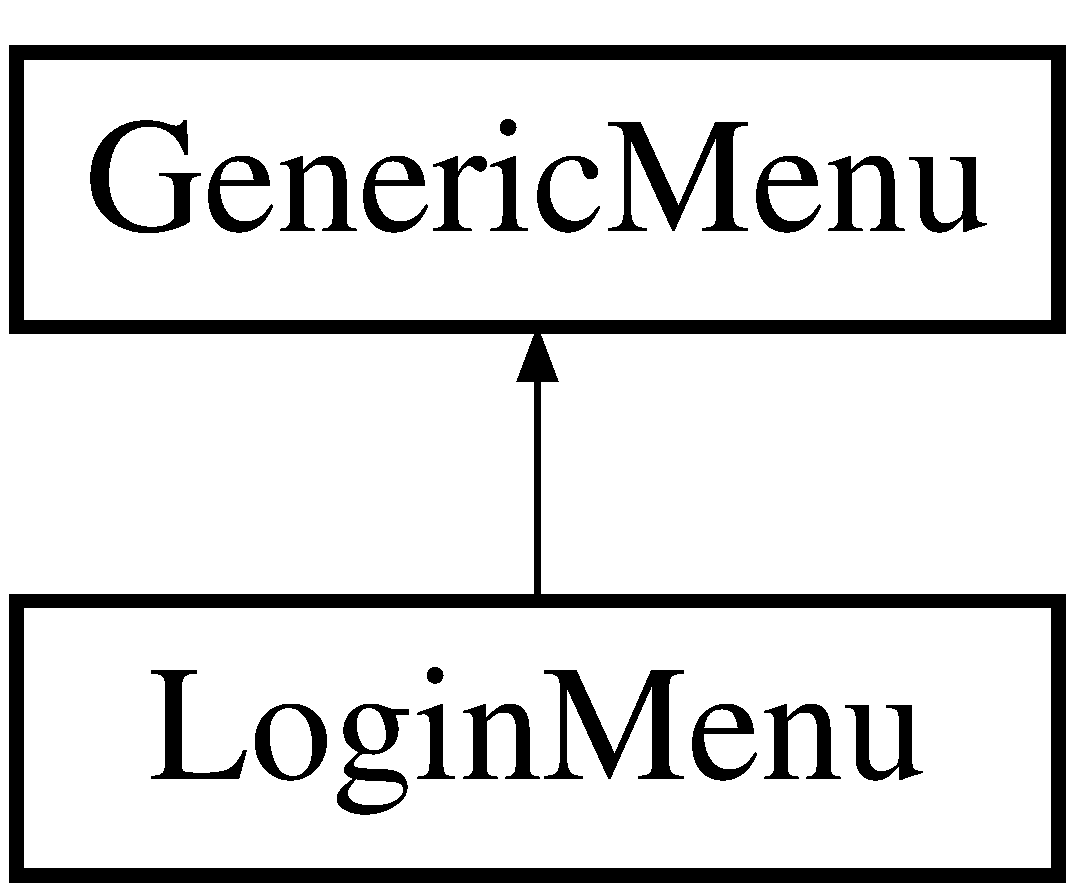
\includegraphics[height=2cm]{classLoginMenu}
\end{center}
\end{figure}
\subsection*{Public Member Functions}
\begin{DoxyCompactItemize}
\item 
\hyperlink{classGenericMenu}{GenericMenu} $\ast$ \hyperlink{classLoginMenu_a2f391af29531a557e0547294e97132fe}{menufunc} (string \&opt, \hyperlink{classstatus}{status} $\ast$\&info)
\begin{DoxyCompactList}\small\item\em menufunc is the general handler for implementing the functionality of this menu class \item\end{DoxyCompactList}\end{DoxyCompactItemize}


\subsection{Member Function Documentation}
\hypertarget{classLoginMenu_a2f391af29531a557e0547294e97132fe}{
\index{LoginMenu@{LoginMenu}!menufunc@{menufunc}}
\index{menufunc@{menufunc}!LoginMenu@{LoginMenu}}
\subsubsection[{menufunc}]{\setlength{\rightskip}{0pt plus 5cm}{\bf GenericMenu} $\ast$ LoginMenu::menufunc (string \& {\em opt}, \/  {\bf status} $\ast$\& {\em info})\hspace{0.3cm}{\ttfamily  \mbox{[}virtual\mbox{]}}}}
\label{classLoginMenu_a2f391af29531a557e0547294e97132fe}


menufunc is the general handler for implementing the functionality of this menu class 
\begin{DoxyParams}{Parameters}
\item[\mbox{$\leftarrow$} {\em opt}]a reference for the program to decide where it must go in the main param\mbox{[}in\mbox{]} \hyperlink{classstatus}{status} is a class to enable manipulation of the current game and players between classes \end{DoxyParams}


Implements \hyperlink{classGenericMenu_a290ad7ec3331edc968190b1d7b48a397}{GenericMenu}.

The documentation for this class was generated from the following files:\begin{DoxyCompactItemize}
\item 
source/Menu/\hyperlink{LoginMenu_8h}{LoginMenu.h}\item 
source/Menu/\hyperlink{LoginMenu_8cc}{LoginMenu.cc}\end{DoxyCompactItemize}

\hypertarget{classMainMenu}{
\section{MainMenu Class Reference}
\label{classMainMenu}\index{MainMenu@{MainMenu}}
}
Inheritance diagram for MainMenu::\begin{figure}[H]
\begin{center}
\leavevmode
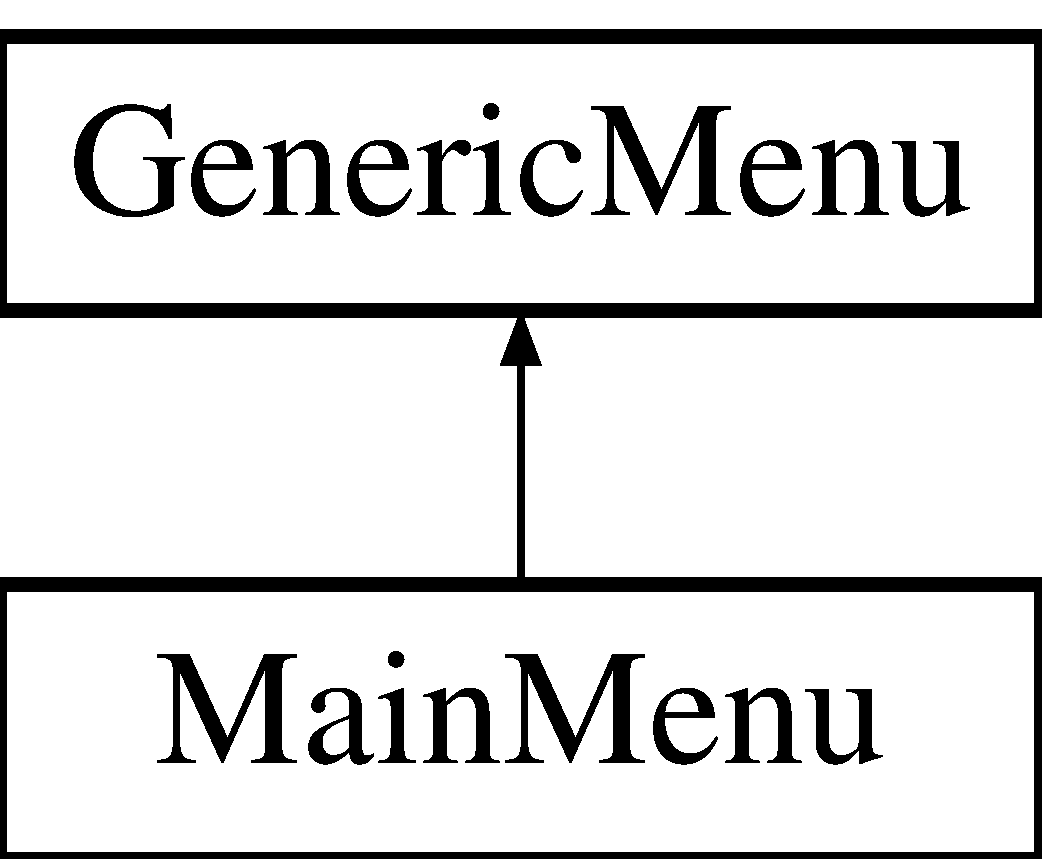
\includegraphics[height=2cm]{classMainMenu}
\end{center}
\end{figure}
\subsection*{Public Member Functions}
\begin{DoxyCompactItemize}
\item 
\hyperlink{classGenericMenu}{GenericMenu} $\ast$ \hyperlink{classMainMenu_aed53ec0c027843a2a1204235fe2924ea}{menufunc} (string \&opt, \hyperlink{classstatus}{status} $\ast$\&info)
\begin{DoxyCompactList}\small\item\em menufunc is the general handler for implementing the functionality of this menu class \item\end{DoxyCompactList}\end{DoxyCompactItemize}


\subsection{Member Function Documentation}
\hypertarget{classMainMenu_aed53ec0c027843a2a1204235fe2924ea}{
\index{MainMenu@{MainMenu}!menufunc@{menufunc}}
\index{menufunc@{menufunc}!MainMenu@{MainMenu}}
\subsubsection[{menufunc}]{\setlength{\rightskip}{0pt plus 5cm}{\bf GenericMenu} $\ast$ MainMenu::menufunc (string \& {\em opt}, \/  {\bf status} $\ast$\& {\em info})\hspace{0.3cm}{\ttfamily  \mbox{[}virtual\mbox{]}}}}
\label{classMainMenu_aed53ec0c027843a2a1204235fe2924ea}


menufunc is the general handler for implementing the functionality of this menu class 
\begin{DoxyParams}{Parameters}
\item[\mbox{$\leftarrow$} {\em opt}]a reference for the program to decide where it must go in the main param\mbox{[}in\mbox{]} \hyperlink{classstatus}{status} is a class to enable manipulation of the current game and players between classes \end{DoxyParams}


Implements \hyperlink{classGenericMenu_a290ad7ec3331edc968190b1d7b48a397}{GenericMenu}.

The documentation for this class was generated from the following files:\begin{DoxyCompactItemize}
\item 
source/Menu/\hyperlink{MainMenu_8h}{MainMenu.h}\item 
source/Menu/\hyperlink{MainMenu_8cc}{MainMenu.cc}\end{DoxyCompactItemize}

\hypertarget{classMemento}{
\section{Memento Class Reference}
\label{classMemento}\index{Memento@{Memento}}
}
\subsection*{Public Member Functions}
\begin{DoxyCompactItemize}
\item 
\hyperlink{classMemento_a00be4fd2d6ba40b9c7e212a64a834f81}{Memento} (int elo=0, int gamesWon=0, int gamesLost=0, int tournamentsWon=0, string name=\char`\"{}Guest\char`\"{})
\begin{DoxyCompactList}\small\item\em creates a memento object for \hyperlink{classRegisteredPlayer}{RegisteredPlayer} class \item\end{DoxyCompactList}\item 
void \hyperlink{classMemento_ae1c59cf9a5ed24dfcbe15d57ee24c095}{writeMemento} (\hyperlink{classMemento}{Memento} $\ast$memento, string fileName)
\begin{DoxyCompactList}\small\item\em writes a memento object to the given osstream \item\end{DoxyCompactList}\item 
\hyperlink{classMemento}{Memento} $\ast$ \hyperlink{classMemento_ad159304bd2710dc9dc9c2ed523075dd0}{readMemento} (string fileName)
\begin{DoxyCompactList}\small\item\em returns a memento object from the given file \item\end{DoxyCompactList}\end{DoxyCompactItemize}
\subsection*{Friends}
\begin{DoxyCompactItemize}
\item 
\hypertarget{classMemento_acb406df94b9d48567f42bbe73b2bd234}{
class \hyperlink{classMemento_acb406df94b9d48567f42bbe73b2bd234}{RegisteredPlayer}}
\label{classMemento_acb406df94b9d48567f42bbe73b2bd234}

\end{DoxyCompactItemize}


\subsection{Constructor \& Destructor Documentation}
\hypertarget{classMemento_a00be4fd2d6ba40b9c7e212a64a834f81}{
\index{Memento@{Memento}!Memento@{Memento}}
\index{Memento@{Memento}!Memento@{Memento}}
\subsubsection[{Memento}]{\setlength{\rightskip}{0pt plus 5cm}Memento::Memento (int {\em elo} = {\ttfamily 0}, \/  int {\em gamesWon} = {\ttfamily 0}, \/  int {\em gamesLost} = {\ttfamily 0}, \/  int {\em tournamentsWon} = {\ttfamily 0}, \/  string {\em name} = {\ttfamily \char`\"{}Guest\char`\"{}})}}
\label{classMemento_a00be4fd2d6ba40b9c7e212a64a834f81}


creates a memento object for \hyperlink{classRegisteredPlayer}{RegisteredPlayer} class 
\begin{DoxyParams}{Parameters}
\item[\mbox{$\leftarrow$} {\em elo}]The elo int to be stored \item[\mbox{$\leftarrow$} {\em gamesWon}]The gamesWon int to be stored \item[\mbox{$\leftarrow$} {\em gamesLost}]The gamesLost int to be stored \item[\mbox{$\leftarrow$} {\em tournamentsWon}]The tournamentsWon int to be stored \end{DoxyParams}


\subsection{Member Function Documentation}
\hypertarget{classMemento_ad159304bd2710dc9dc9c2ed523075dd0}{
\index{Memento@{Memento}!readMemento@{readMemento}}
\index{readMemento@{readMemento}!Memento@{Memento}}
\subsubsection[{readMemento}]{\setlength{\rightskip}{0pt plus 5cm}{\bf Memento} $\ast$ Memento::readMemento (string {\em fileName})}}
\label{classMemento_ad159304bd2710dc9dc9c2ed523075dd0}


returns a memento object from the given file 
\begin{DoxyParams}{Parameters}
\item[\mbox{$\leftarrow$} {\em fileName}]a string for the file the memento object is read from \end{DoxyParams}
\begin{DoxyReturn}{Returns}
the memento object that is read from file 
\end{DoxyReturn}
\hypertarget{classMemento_ae1c59cf9a5ed24dfcbe15d57ee24c095}{
\index{Memento@{Memento}!writeMemento@{writeMemento}}
\index{writeMemento@{writeMemento}!Memento@{Memento}}
\subsubsection[{writeMemento}]{\setlength{\rightskip}{0pt plus 5cm}void Memento::writeMemento ({\bf Memento} $\ast$ {\em memento}, \/  string {\em fileName})}}
\label{classMemento_ae1c59cf9a5ed24dfcbe15d57ee24c095}


writes a memento object to the given osstream 
\begin{DoxyParams}{Parameters}
\item[\mbox{$\leftarrow$} {\em os}]the output stream to write the memento object to.(probably filestream) \item[\mbox{$\leftarrow$} {\em fileName}]a string for the file the memento object is written to \end{DoxyParams}


The documentation for this class was generated from the following files:\begin{DoxyCompactItemize}
\item 
source/Players/Player.h\item 
source/Players/Player.cc\end{DoxyCompactItemize}

\hypertarget{classNotEnoughPieces}{
\section{NotEnoughPieces Class Reference}
\label{classNotEnoughPieces}\index{NotEnoughPieces@{NotEnoughPieces}}
}
Inheritance diagram for NotEnoughPieces::\begin{figure}[H]
\begin{center}
\leavevmode
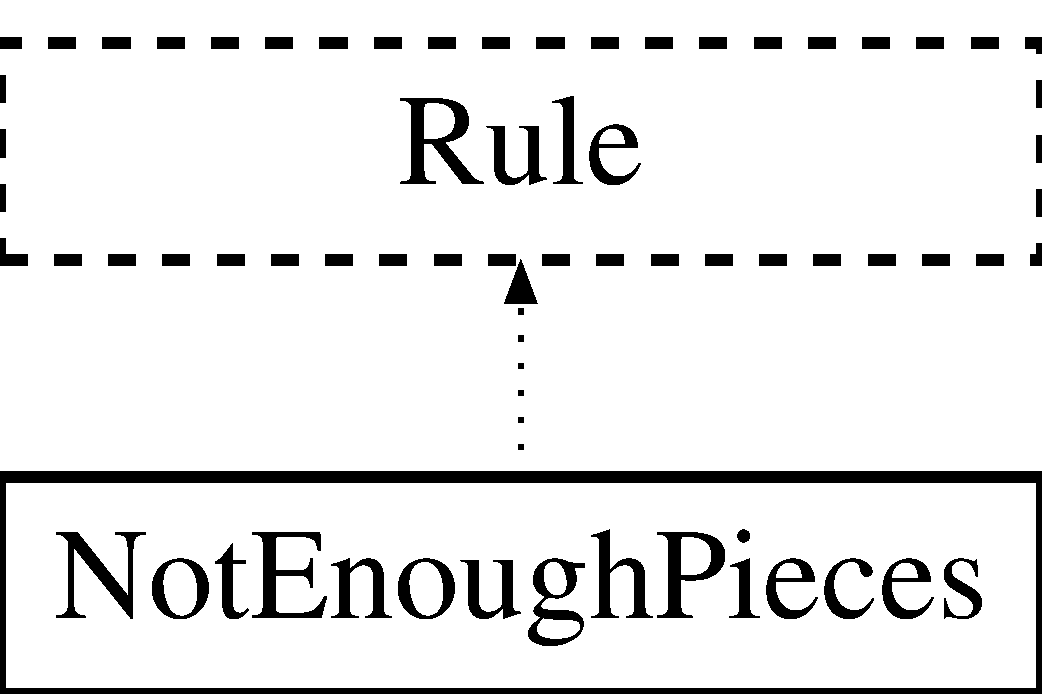
\includegraphics[height=2cm]{classNotEnoughPieces}
\end{center}
\end{figure}
\subsection*{Public Member Functions}
\begin{DoxyCompactItemize}
\item 
\hyperlink{classNotEnoughPieces_a854f2be1fd97be94a879d50c6e64f277}{NotEnoughPieces} ()
\begin{DoxyCompactList}\small\item\em \hyperlink{classNotEnoughPieces}{NotEnoughPieces} creates a \hyperlink{classNotEnoughPieces}{NotEnoughPieces} object. \item\end{DoxyCompactList}\item 
\hypertarget{classNotEnoughPieces_a30f5c2c61a8ba12a692dc818a8e99e49}{
int \hyperlink{classNotEnoughPieces_a30f5c2c61a8ba12a692dc818a8e99e49}{validMove} (vector$<$ vector$<$ \hyperlink{classPiece}{Piece} $\ast$ $>$ $>$ \&b, int ix, int iy, int dx, int dy)}
\label{classNotEnoughPieces_a30f5c2c61a8ba12a692dc818a8e99e49}

\begin{DoxyCompactList}\small\item\em validMove checks if the pieces left alive are the bishop and king or the knight and king it will return 2 else return 1. \item\end{DoxyCompactList}\end{DoxyCompactItemize}


\subsection{Constructor \& Destructor Documentation}
\hypertarget{classNotEnoughPieces_a854f2be1fd97be94a879d50c6e64f277}{
\index{NotEnoughPieces@{NotEnoughPieces}!NotEnoughPieces@{NotEnoughPieces}}
\index{NotEnoughPieces@{NotEnoughPieces}!NotEnoughPieces@{NotEnoughPieces}}
\subsubsection[{NotEnoughPieces}]{\setlength{\rightskip}{0pt plus 5cm}NotEnoughPieces::NotEnoughPieces ()}}
\label{classNotEnoughPieces_a854f2be1fd97be94a879d50c6e64f277}


\hyperlink{classNotEnoughPieces}{NotEnoughPieces} creates a \hyperlink{classNotEnoughPieces}{NotEnoughPieces} object. 
\begin{DoxyParams}{Parameters}
\item[\mbox{$\leftarrow$} {\em b}]is a vector$<$ vector $<$ Piece$\ast$ $>$ $>$ object \item[\mbox{$\leftarrow$} {\em ix}]is the x for the initial location \item[\mbox{$\leftarrow$} {\em iy}]is the y for the initial location \item[\mbox{$\leftarrow$} {\em dx}]is the x for the destination location \item[\mbox{$\leftarrow$} {\em dy}]is the y for the destination location \end{DoxyParams}


The documentation for this class was generated from the following files:\begin{DoxyCompactItemize}
\item 
source/Rules/\hyperlink{NotEnoughPieces_8h}{NotEnoughPieces.h}\item 
source/Rules/NotEnoughPieces.cc\end{DoxyCompactItemize}

\hypertarget{classPauseMenu}{
\section{PauseMenu Class Reference}
\label{classPauseMenu}\index{PauseMenu@{PauseMenu}}
}


\hyperlink{classPauseMenu}{PauseMenu} is a subclass of Generic Menu.  


{\ttfamily \#include $<$PauseMenu.h$>$}Inheritance diagram for PauseMenu::\begin{figure}[H]
\begin{center}
\leavevmode
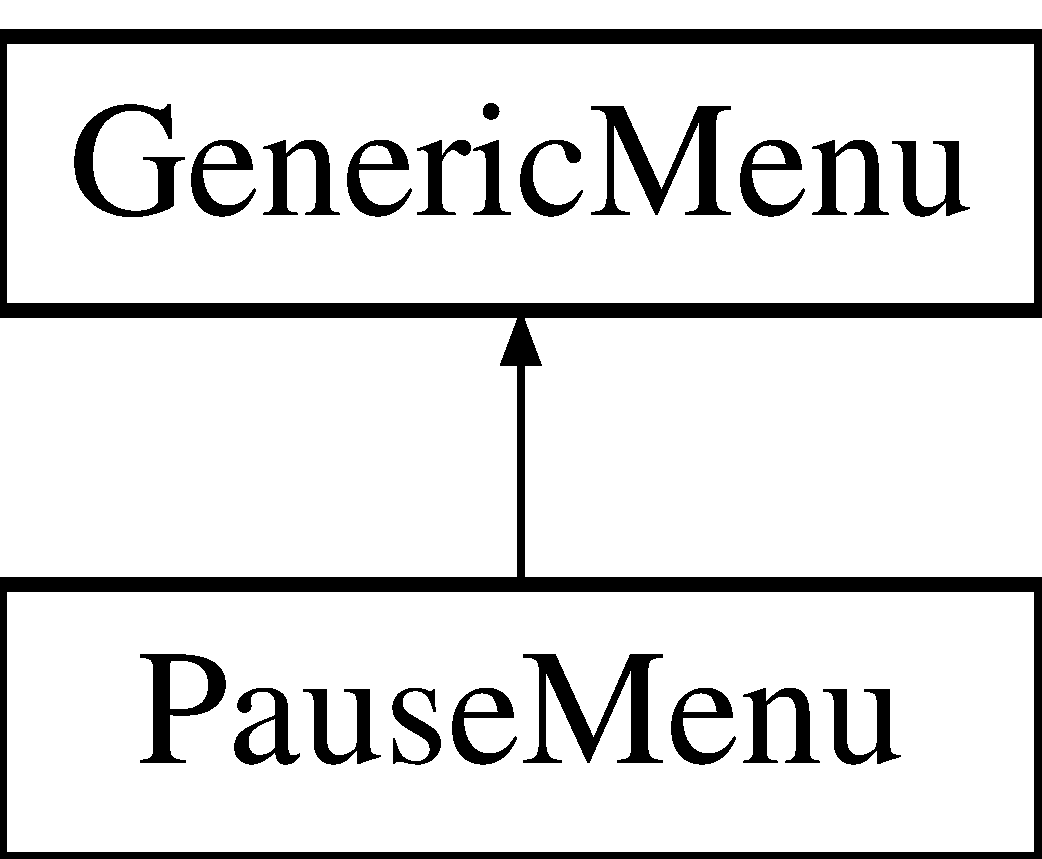
\includegraphics[height=2cm]{classPauseMenu}
\end{center}
\end{figure}
\subsection*{Public Member Functions}
\begin{DoxyCompactItemize}
\item 
\hypertarget{classPauseMenu_ae7b38f4044988404e1502245ee7438d3}{
\hyperlink{classPauseMenu_ae7b38f4044988404e1502245ee7438d3}{PauseMenu} ()}
\label{classPauseMenu_ae7b38f4044988404e1502245ee7438d3}

\begin{DoxyCompactList}\small\item\em \hyperlink{classPauseMenu}{PauseMenu} intializes all the buttons and assigns the buttons a sprite. \item\end{DoxyCompactList}\item 
\hyperlink{classGenericMenu}{GenericMenu} $\ast$ \hyperlink{classPauseMenu_a7926ffe9dd0aa74281d8cb8126cd9c10}{menufunc} (string \&opt, \hyperlink{classstatus}{status} $\ast$\&info)
\begin{DoxyCompactList}\small\item\em menufunc is the general handler for implementing the functionality of this menu class \item\end{DoxyCompactList}\end{DoxyCompactItemize}


\subsection{Detailed Description}
\hyperlink{classPauseMenu}{PauseMenu} is a subclass of Generic Menu. 

\subsection{Member Function Documentation}
\hypertarget{classPauseMenu_a7926ffe9dd0aa74281d8cb8126cd9c10}{
\index{PauseMenu@{PauseMenu}!menufunc@{menufunc}}
\index{menufunc@{menufunc}!PauseMenu@{PauseMenu}}
\subsubsection[{menufunc}]{\setlength{\rightskip}{0pt plus 5cm}{\bf GenericMenu} $\ast$ PauseMenu::menufunc (string \& {\em opt}, \/  {\bf status} $\ast$\& {\em info})\hspace{0.3cm}{\ttfamily  \mbox{[}virtual\mbox{]}}}}
\label{classPauseMenu_a7926ffe9dd0aa74281d8cb8126cd9c10}


menufunc is the general handler for implementing the functionality of this menu class 
\begin{DoxyParams}{Parameters}
\item[\mbox{$\leftarrow$} {\em opt}]a reference for the program to decide where it must go in the main param\mbox{[}in\mbox{]} \hyperlink{classstatus}{status} is a class to enable manipulation of the current game and players between classes \end{DoxyParams}


Implements \hyperlink{classGenericMenu_a290ad7ec3331edc968190b1d7b48a397}{GenericMenu}.

The documentation for this class was generated from the following files:\begin{DoxyCompactItemize}
\item 
source/Menu/\hyperlink{PauseMenu_8h}{PauseMenu.h}\item 
source/Menu/\hyperlink{PauseMenu_8cc}{PauseMenu.cc}\end{DoxyCompactItemize}

\hypertarget{classPawnCapture}{
\section{PawnCapture Class Reference}
\label{classPawnCapture}\index{PawnCapture@{PawnCapture}}
}
Inheritance diagram for PawnCapture::\begin{figure}[H]
\begin{center}
\leavevmode
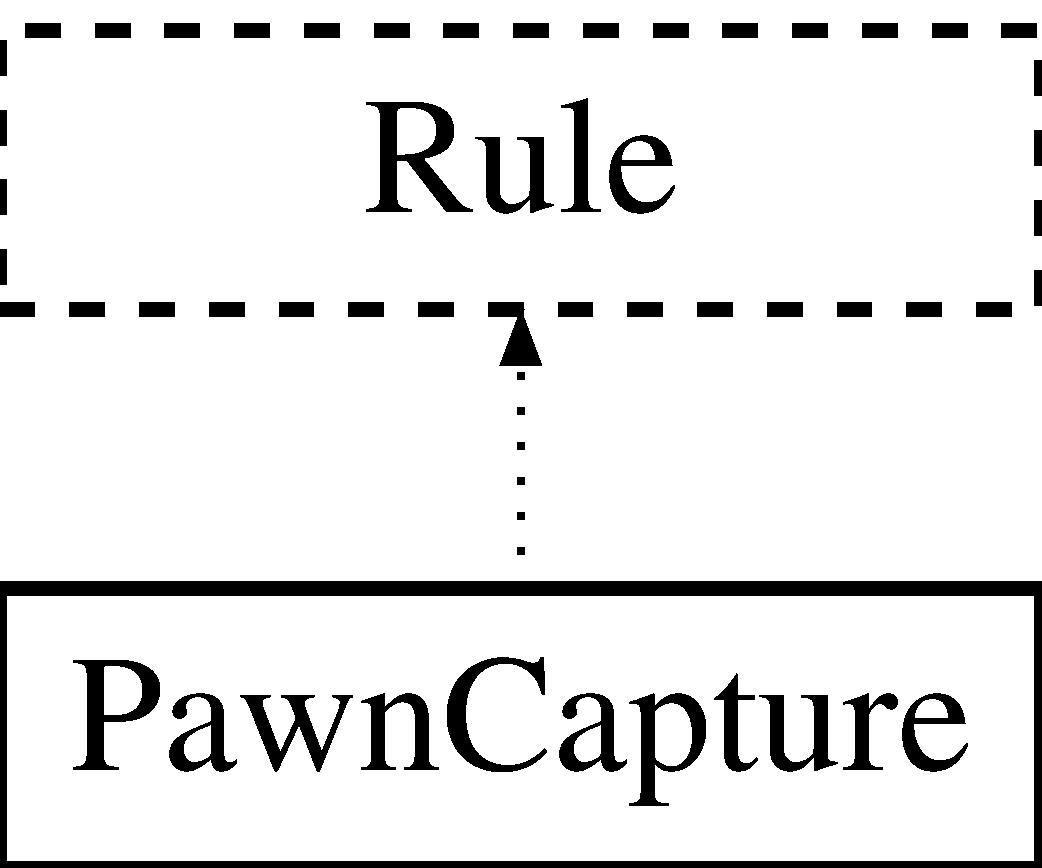
\includegraphics[height=2cm]{classPawnCapture}
\end{center}
\end{figure}
\subsection*{Public Member Functions}
\begin{DoxyCompactItemize}
\item 
\hyperlink{classPawnCapture_a1d47980f9be9650f3d4201d417aaaec2}{PawnCapture} ()
\begin{DoxyCompactList}\small\item\em \hyperlink{classPawnCapture}{PawnCapture} creates a \hyperlink{classPawnCapture}{PawnCapture} object. \item\end{DoxyCompactList}\item 
int \hyperlink{classPawnCapture_afa1faa171cb70974f46add5989c3f373}{validMove} (vector$<$ vector$<$ \hyperlink{classPiece}{Piece} $\ast$ $>$ $>$ \&b, int ix, int iy, int dx, int dy)
\begin{DoxyCompactList}\small\item\em validMove if the player is trying to move forward go to promotion class. if that is false, check if there is an valid attack for pawn, return 1 else return 0. \item\end{DoxyCompactList}\end{DoxyCompactItemize}


\subsection{Constructor \& Destructor Documentation}
\hypertarget{classPawnCapture_a1d47980f9be9650f3d4201d417aaaec2}{
\index{PawnCapture@{PawnCapture}!PawnCapture@{PawnCapture}}
\index{PawnCapture@{PawnCapture}!PawnCapture@{PawnCapture}}
\subsubsection[{PawnCapture}]{\setlength{\rightskip}{0pt plus 5cm}PawnCapture::PawnCapture ()}}
\label{classPawnCapture_a1d47980f9be9650f3d4201d417aaaec2}


\hyperlink{classPawnCapture}{PawnCapture} creates a \hyperlink{classPawnCapture}{PawnCapture} object. 
\begin{DoxyParams}{Parameters}
\item[\mbox{$\leftarrow$} {\em b}]is a vector$<$ vector $<$ Piece$\ast$ $>$ $>$ object \item[\mbox{$\leftarrow$} {\em ix}]is the x for the initial location \item[\mbox{$\leftarrow$} {\em iy}]is the y for the initial location \item[\mbox{$\leftarrow$} {\em dx}]is the x for the destination location \item[\mbox{$\leftarrow$} {\em dy}]is the y for the destination location \end{DoxyParams}


\subsection{Member Function Documentation}
\hypertarget{classPawnCapture_afa1faa171cb70974f46add5989c3f373}{
\index{PawnCapture@{PawnCapture}!validMove@{validMove}}
\index{validMove@{validMove}!PawnCapture@{PawnCapture}}
\subsubsection[{validMove}]{\setlength{\rightskip}{0pt plus 5cm}int PawnCapture::validMove (vector$<$ vector$<$ {\bf Piece} $\ast$ $>$ $>$ \& {\em b}, \/  int {\em ix}, \/  int {\em iy}, \/  int {\em dx}, \/  int {\em dy})\hspace{0.3cm}{\ttfamily  \mbox{[}virtual\mbox{]}}}}
\label{classPawnCapture_afa1faa171cb70974f46add5989c3f373}


validMove if the player is trying to move forward go to promotion class. if that is false, check if there is an valid attack for pawn, return 1 else return 0. \begin{DoxyReturn}{Returns}
an int 
\end{DoxyReturn}


Implements \hyperlink{classRule}{Rule}.

The documentation for this class was generated from the following files:\begin{DoxyCompactItemize}
\item 
source/Rules/\hyperlink{PawnCapture_8h}{PawnCapture.h}\item 
source/Rules/PawnCapture.cc\end{DoxyCompactItemize}

\hypertarget{classPawnMove}{
\section{PawnMove Class Reference}
\label{classPawnMove}\index{PawnMove@{PawnMove}}
}
Inheritance diagram for PawnMove::\begin{figure}[H]
\begin{center}
\leavevmode
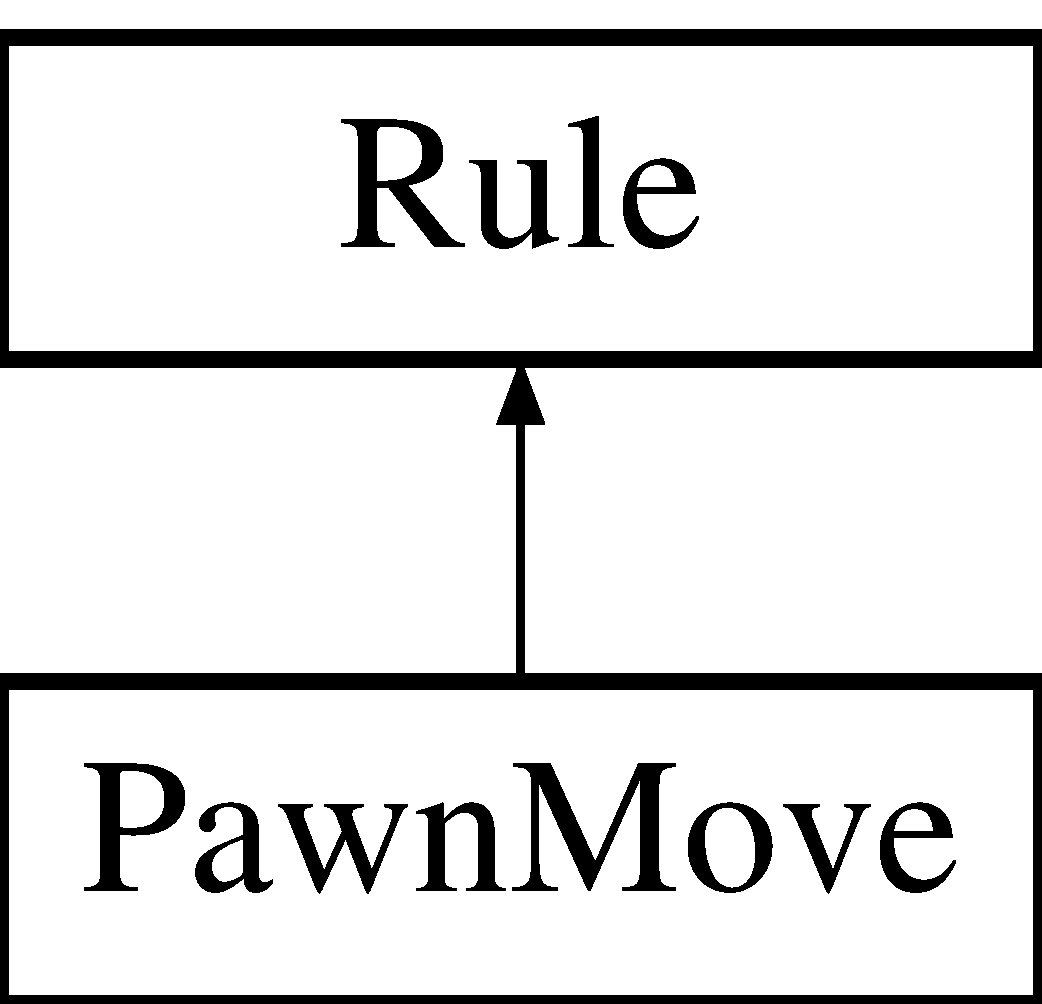
\includegraphics[height=2cm]{classPawnMove}
\end{center}
\end{figure}
\subsection*{Public Member Functions}
\begin{DoxyCompactItemize}
\item 
\hyperlink{classPawnMove_ab0b45a34a1c124f8f852ad6ce512bdcc}{PawnMove} ()
\begin{DoxyCompactList}\small\item\em \hyperlink{classPawnMove}{PawnMove} creates a \hyperlink{classPawnMove}{PawnMove} object. \item\end{DoxyCompactList}\item 
int \hyperlink{classPawnMove_a9280b4befe12bc9439d60ad7765187af}{validMove} (vector$<$ vector$<$ \hyperlink{classPiece}{Piece} $\ast$ $>$ $>$ \&b, int ix, int iy, int dx, int dy)
\begin{DoxyCompactList}\small\item\em validMove checks if the move made by the user is a valid move or Pawns to make. if invalid calls \hyperlink{classPawnCapture}{PawnCapture}. if invalid return 0. \item\end{DoxyCompactList}\end{DoxyCompactItemize}


\subsection{Constructor \& Destructor Documentation}
\hypertarget{classPawnMove_ab0b45a34a1c124f8f852ad6ce512bdcc}{
\index{PawnMove@{PawnMove}!PawnMove@{PawnMove}}
\index{PawnMove@{PawnMove}!PawnMove@{PawnMove}}
\subsubsection[{PawnMove}]{\setlength{\rightskip}{0pt plus 5cm}PawnMove::PawnMove ()}}
\label{classPawnMove_ab0b45a34a1c124f8f852ad6ce512bdcc}


\hyperlink{classPawnMove}{PawnMove} creates a \hyperlink{classPawnMove}{PawnMove} object. 
\begin{DoxyParams}{Parameters}
\item[\mbox{$\leftarrow$} {\em b}]is a vector$<$ vector $<$ Piece$\ast$ $>$ $>$ object \item[\mbox{$\leftarrow$} {\em ix}]is the x for the initial location \item[\mbox{$\leftarrow$} {\em iy}]is the y for the initial location \item[\mbox{$\leftarrow$} {\em dx}]is the x for the destination location \item[\mbox{$\leftarrow$} {\em dy}]is the y for the destination location \end{DoxyParams}


\subsection{Member Function Documentation}
\hypertarget{classPawnMove_a9280b4befe12bc9439d60ad7765187af}{
\index{PawnMove@{PawnMove}!validMove@{validMove}}
\index{validMove@{validMove}!PawnMove@{PawnMove}}
\subsubsection[{validMove}]{\setlength{\rightskip}{0pt plus 5cm}int PawnMove::validMove (vector$<$ vector$<$ {\bf Piece} $\ast$ $>$ $>$ \& {\em b}, \/  int {\em ix}, \/  int {\em iy}, \/  int {\em dx}, \/  int {\em dy})\hspace{0.3cm}{\ttfamily  \mbox{[}virtual\mbox{]}}}}
\label{classPawnMove_a9280b4befe12bc9439d60ad7765187af}


validMove checks if the move made by the user is a valid move or Pawns to make. if invalid calls \hyperlink{classPawnCapture}{PawnCapture}. if invalid return 0. \begin{DoxyReturn}{Returns}
an int 
\end{DoxyReturn}


Implements \hyperlink{classRule}{Rule}.

The documentation for this class was generated from the following files:\begin{DoxyCompactItemize}
\item 
source/Rules/\hyperlink{PawnMove_8h}{PawnMove.h}\item 
source/Rules/PawnMove.cc\end{DoxyCompactItemize}

\hypertarget{classPawnPiece}{
\section{PawnPiece Class Reference}
\label{classPawnPiece}\index{PawnPiece@{PawnPiece}}
}


a class for all Pawn Piece`s.  


{\ttfamily \#include $<$PawnPiece.h$>$}Inheritance diagram for PawnPiece::\begin{figure}[H]
\begin{center}
\leavevmode
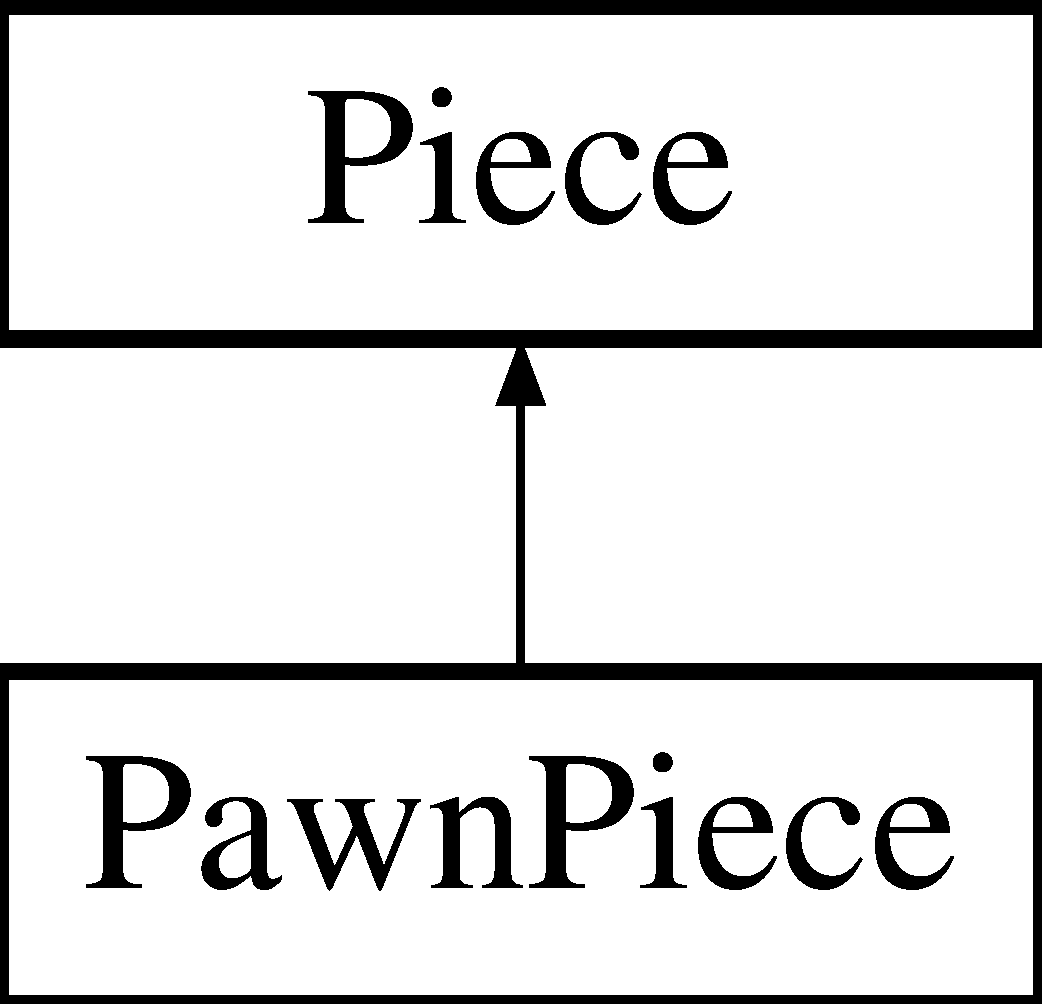
\includegraphics[height=2cm]{classPawnPiece}
\end{center}
\end{figure}
\subsection*{Public Member Functions}
\begin{DoxyCompactItemize}
\item 
\hypertarget{classPawnPiece_ab4120d3c4881559475326efdb1348d45}{
\hyperlink{classPawnPiece_ab4120d3c4881559475326efdb1348d45}{PawnPiece} (int c=0)}
\label{classPawnPiece_ab4120d3c4881559475326efdb1348d45}

\begin{DoxyCompactList}\small\item\em creates a \hyperlink{classPiece}{Piece} object \item\end{DoxyCompactList}\item 
int \hyperlink{classPawnPiece_abe56912427ff110820b34223e5f60cda}{getColor} () const 
\begin{DoxyCompactList}\small\item\em gets the color of the Pawn \hyperlink{classPiece}{Piece} \item\end{DoxyCompactList}\item 
void \hyperlink{classPawnPiece_a5cfd7bce3cea8ad32c1b8dc8f5c7b253}{setColor} (int colorOfPiece)
\begin{DoxyCompactList}\small\item\em sets the Color of the Pawn \hyperlink{classPiece}{Piece} \item\end{DoxyCompactList}\item 
string \hyperlink{classPawnPiece_a0a612a59fd7bb512805329902e829ce6}{getType} () const 
\begin{DoxyCompactList}\small\item\em Returns Pawn to user. \item\end{DoxyCompactList}\item 
virtual int \hyperlink{classPawnPiece_a693be3f65626d084104215482619efbf}{validMove} (vector$<$ vector$<$ \hyperlink{classPiece}{Piece} $\ast$ $>$ $>$ gameBoard, int ix, int iy, int dx, int dy)
\begin{DoxyCompactList}\small\item\em validates a move based on the Pawn rules. \item\end{DoxyCompactList}\end{DoxyCompactItemize}


\subsection{Detailed Description}
a class for all Pawn Piece`s. 

\subsection{Member Function Documentation}
\hypertarget{classPawnPiece_abe56912427ff110820b34223e5f60cda}{
\index{PawnPiece@{PawnPiece}!getColor@{getColor}}
\index{getColor@{getColor}!PawnPiece@{PawnPiece}}
\subsubsection[{getColor}]{\setlength{\rightskip}{0pt plus 5cm}int PawnPiece::getColor () const\hspace{0.3cm}{\ttfamily  \mbox{[}virtual\mbox{]}}}}
\label{classPawnPiece_abe56912427ff110820b34223e5f60cda}


gets the color of the Pawn \hyperlink{classPiece}{Piece} \begin{DoxyReturn}{Returns}
int a 0 if white and 1 if black 
\end{DoxyReturn}


Implements \hyperlink{classPiece_a1376072d4815719e60253ce5688df95c}{Piece}.\hypertarget{classPawnPiece_a0a612a59fd7bb512805329902e829ce6}{
\index{PawnPiece@{PawnPiece}!getType@{getType}}
\index{getType@{getType}!PawnPiece@{PawnPiece}}
\subsubsection[{getType}]{\setlength{\rightskip}{0pt plus 5cm}string PawnPiece::getType () const\hspace{0.3cm}{\ttfamily  \mbox{[}virtual\mbox{]}}}}
\label{classPawnPiece_a0a612a59fd7bb512805329902e829ce6}


Returns Pawn to user. \begin{DoxyReturn}{Returns}
a string that will return Pawn Type. 
\end{DoxyReturn}


Implements \hyperlink{classPiece_a5b88fcd786bb30b345b24fbc3ab24ab9}{Piece}.\hypertarget{classPawnPiece_a5cfd7bce3cea8ad32c1b8dc8f5c7b253}{
\index{PawnPiece@{PawnPiece}!setColor@{setColor}}
\index{setColor@{setColor}!PawnPiece@{PawnPiece}}
\subsubsection[{setColor}]{\setlength{\rightskip}{0pt plus 5cm}void PawnPiece::setColor (int {\em colorOfPiece})\hspace{0.3cm}{\ttfamily  \mbox{[}virtual\mbox{]}}}}
\label{classPawnPiece_a5cfd7bce3cea8ad32c1b8dc8f5c7b253}


sets the Color of the Pawn \hyperlink{classPiece}{Piece} 
\begin{DoxyParams}{Parameters}
\item[\mbox{$\leftarrow$} {\em colorOfPiece}]sets the Pawn Piece`s color \end{DoxyParams}


Implements \hyperlink{classPiece_a1387cb503dca308ac1e3bbe38a70a073}{Piece}.\hypertarget{classPawnPiece_a693be3f65626d084104215482619efbf}{
\index{PawnPiece@{PawnPiece}!validMove@{validMove}}
\index{validMove@{validMove}!PawnPiece@{PawnPiece}}
\subsubsection[{validMove}]{\setlength{\rightskip}{0pt plus 5cm}virtual int PawnPiece::validMove (vector$<$ vector$<$ {\bf Piece} $\ast$ $>$ $>$ {\em gameBoard}, \/  int {\em ix}, \/  int {\em iy}, \/  int {\em dx}, \/  int {\em dy})\hspace{0.3cm}{\ttfamily  \mbox{[}virtual\mbox{]}}}}
\label{classPawnPiece_a693be3f65626d084104215482619efbf}


validates a move based on the Pawn rules. 
\begin{DoxyParams}{Parameters}
\item[\mbox{$\leftarrow$} {\em board}]A \hyperlink{classBoard}{Board} that will contain the currect board state \item[\mbox{$\leftarrow$} {\em ix}]A int that holds the x coordinate of where the piece is moving from \item[\mbox{$\leftarrow$} {\em iy}]A int that holds the y coordinate of where the piece is moving from \item[\mbox{$\leftarrow$} {\em dx}]A int that holds the x coordinate of where the piece is moving to \item[\mbox{$\leftarrow$} {\em dy}]A int that holds the y coordinate of where the piece is moving to \end{DoxyParams}


The documentation for this class was generated from the following files:\begin{DoxyCompactItemize}
\item 
source/Piece/\hyperlink{PawnPiece_8h}{PawnPiece.h}\item 
source/Piece/PawnPiece.cc\end{DoxyCompactItemize}

\hypertarget{classPiece}{
\section{Piece Class Reference}
\label{classPiece}\index{Piece@{Piece}}
}


a a base class that will be inherited by all other Piece`s.  


{\ttfamily \#include $<$Piece.h$>$}Inheritance diagram for Piece::\begin{figure}[H]
\begin{center}
\leavevmode
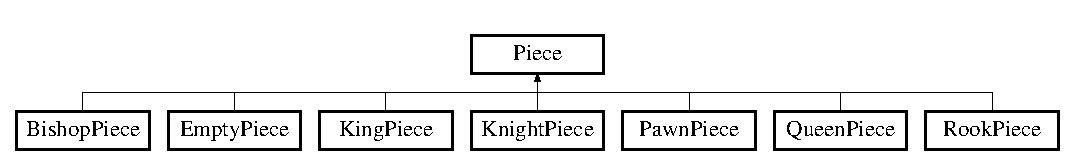
\includegraphics[height=1.77778cm]{classPiece}
\end{center}
\end{figure}
\subsection*{Public Member Functions}
\begin{DoxyCompactItemize}
\item 
virtual int \hyperlink{classPiece_a1376072d4815719e60253ce5688df95c}{getColor} () const =0
\begin{DoxyCompactList}\small\item\em gets the color of the \hyperlink{classPiece}{Piece} \item\end{DoxyCompactList}\item 
virtual void \hyperlink{classPiece_a1387cb503dca308ac1e3bbe38a70a073}{setColor} (int colorOfPiece)=0
\begin{DoxyCompactList}\small\item\em sets the Color of the \hyperlink{classPiece}{Piece} \item\end{DoxyCompactList}\item 
virtual string \hyperlink{classPiece_a5b88fcd786bb30b345b24fbc3ab24ab9}{getType} () const =0
\begin{DoxyCompactList}\small\item\em gets the type of \hyperlink{classPiece}{Piece} \item\end{DoxyCompactList}\item 
virtual int \hyperlink{classPiece_a6bc81a2d7211e5a7972cec0a34ebb473}{validMove} (vector$<$ vector$<$ \hyperlink{classPiece}{Piece} $\ast$ $>$ $>$ gameBoard, int ix, int iy, int dx, int dy)=0
\begin{DoxyCompactList}\small\item\em validates a move based on the Pieces Move attribute. This will be overwritten \item\end{DoxyCompactList}\end{DoxyCompactItemize}


\subsection{Detailed Description}
a a base class that will be inherited by all other Piece`s. 

\subsection{Member Function Documentation}
\hypertarget{classPiece_a1376072d4815719e60253ce5688df95c}{
\index{Piece@{Piece}!getColor@{getColor}}
\index{getColor@{getColor}!Piece@{Piece}}
\subsubsection[{getColor}]{\setlength{\rightskip}{0pt plus 5cm}virtual int Piece::getColor () const\hspace{0.3cm}{\ttfamily  \mbox{[}pure virtual\mbox{]}}}}
\label{classPiece_a1376072d4815719e60253ce5688df95c}


gets the color of the \hyperlink{classPiece}{Piece} \begin{DoxyReturn}{Returns}
int a 0 if white and 1 if black 
\end{DoxyReturn}


Implemented in \hyperlink{classBishopPiece_ae40042d8edb9172b97955a1a3d651434}{BishopPiece}, \hyperlink{classEmptyPiece_aa0ae8e05e0471cf05e17bc9f56e30188}{EmptyPiece}, \hyperlink{classKingPiece_ac15e38c6ceaccae6879ec70211c2ab28}{KingPiece}, \hyperlink{classKnightPiece_ab8ef95a1a625e461ada96e4692599770}{KnightPiece}, \hyperlink{classPawnPiece_abe56912427ff110820b34223e5f60cda}{PawnPiece}, \hyperlink{classQueenPiece_a461d58f951b5e9f4d120cec0c47a1d9c}{QueenPiece}, and \hyperlink{classRookPiece_a15b00afd7fe0fe1035c64b884870c6e1}{RookPiece}.\hypertarget{classPiece_a5b88fcd786bb30b345b24fbc3ab24ab9}{
\index{Piece@{Piece}!getType@{getType}}
\index{getType@{getType}!Piece@{Piece}}
\subsubsection[{getType}]{\setlength{\rightskip}{0pt plus 5cm}virtual string Piece::getType () const\hspace{0.3cm}{\ttfamily  \mbox{[}pure virtual\mbox{]}}}}
\label{classPiece_a5b88fcd786bb30b345b24fbc3ab24ab9}


gets the type of \hyperlink{classPiece}{Piece} \begin{DoxyReturn}{Returns}
a string that will be the \hyperlink{classPiece}{Piece} Type. 
\end{DoxyReturn}


Implemented in \hyperlink{classBishopPiece_af651439e984e4d28955db75da601b35b}{BishopPiece}, \hyperlink{classEmptyPiece_ad71f9165591337d5df65c4f2500e2d36}{EmptyPiece}, \hyperlink{classKingPiece_ac93de53a7adee6e5ad33284f0fd6aa2e}{KingPiece}, \hyperlink{classKnightPiece_a3b141e4014d09bba70625ccb2129efcc}{KnightPiece}, \hyperlink{classPawnPiece_a0a612a59fd7bb512805329902e829ce6}{PawnPiece}, \hyperlink{classQueenPiece_ae8df61c033b58d7f96e344166a9f2bdb}{QueenPiece}, and \hyperlink{classRookPiece_a45d8858e75e550b72d27d49da0230c0a}{RookPiece}.\hypertarget{classPiece_a1387cb503dca308ac1e3bbe38a70a073}{
\index{Piece@{Piece}!setColor@{setColor}}
\index{setColor@{setColor}!Piece@{Piece}}
\subsubsection[{setColor}]{\setlength{\rightskip}{0pt plus 5cm}virtual void Piece::setColor (int {\em colorOfPiece})\hspace{0.3cm}{\ttfamily  \mbox{[}pure virtual\mbox{]}}}}
\label{classPiece_a1387cb503dca308ac1e3bbe38a70a073}


sets the Color of the \hyperlink{classPiece}{Piece} 
\begin{DoxyParams}{Parameters}
\item[\mbox{$\leftarrow$} {\em colorOfPiece}]sets the \hyperlink{classPiece}{Piece} color \end{DoxyParams}


Implemented in \hyperlink{classBishopPiece_ae75166e3d3bc71f3030268158cba4054}{BishopPiece}, \hyperlink{classEmptyPiece_ae46e7ddf6275c1508528e06929cf2660}{EmptyPiece}, \hyperlink{classKingPiece_ab7a9023dda46c21a566675623f1b4a32}{KingPiece}, \hyperlink{classKnightPiece_a928091c9100f4e3bc2bb2d10535ccc49}{KnightPiece}, \hyperlink{classPawnPiece_a5cfd7bce3cea8ad32c1b8dc8f5c7b253}{PawnPiece}, \hyperlink{classQueenPiece_a691ff6afc7d167dab9cff0c910cae859}{QueenPiece}, and \hyperlink{classRookPiece_ad10584bf27bf3f6f109074b878ef840d}{RookPiece}.\hypertarget{classPiece_a6bc81a2d7211e5a7972cec0a34ebb473}{
\index{Piece@{Piece}!validMove@{validMove}}
\index{validMove@{validMove}!Piece@{Piece}}
\subsubsection[{validMove}]{\setlength{\rightskip}{0pt plus 5cm}virtual int Piece::validMove (vector$<$ vector$<$ {\bf Piece} $\ast$ $>$ $>$ {\em gameBoard}, \/  int {\em ix}, \/  int {\em iy}, \/  int {\em dx}, \/  int {\em dy})\hspace{0.3cm}{\ttfamily  \mbox{[}pure virtual\mbox{]}}}}
\label{classPiece_a6bc81a2d7211e5a7972cec0a34ebb473}


validates a move based on the Pieces Move attribute. This will be overwritten 
\begin{DoxyParams}{Parameters}
\item[\mbox{$\leftarrow$} {\em board}]A \hyperlink{classBoard}{Board} that will contain the currect board state \item[\mbox{$\leftarrow$} {\em ix}]A int that holds the x coordinate of where the piece is moving from \item[\mbox{$\leftarrow$} {\em iy}]A int that holds the y coordinate of where the piece is moving from \item[\mbox{$\leftarrow$} {\em dx}]A int that holds the x coordinate of where the piece is moving to \item[\mbox{$\leftarrow$} {\em dy}]A int that holds the y coordinate of where the piece is moving to \end{DoxyParams}


The documentation for this class was generated from the following file:\begin{DoxyCompactItemize}
\item 
source/Piece/\hyperlink{Piece_8h}{Piece.h}\end{DoxyCompactItemize}

\hypertarget{classPieceInWay}{
\section{PieceInWay Class Reference}
\label{classPieceInWay}\index{PieceInWay@{PieceInWay}}
}
Inheritance diagram for PieceInWay::\begin{figure}[H]
\begin{center}
\leavevmode
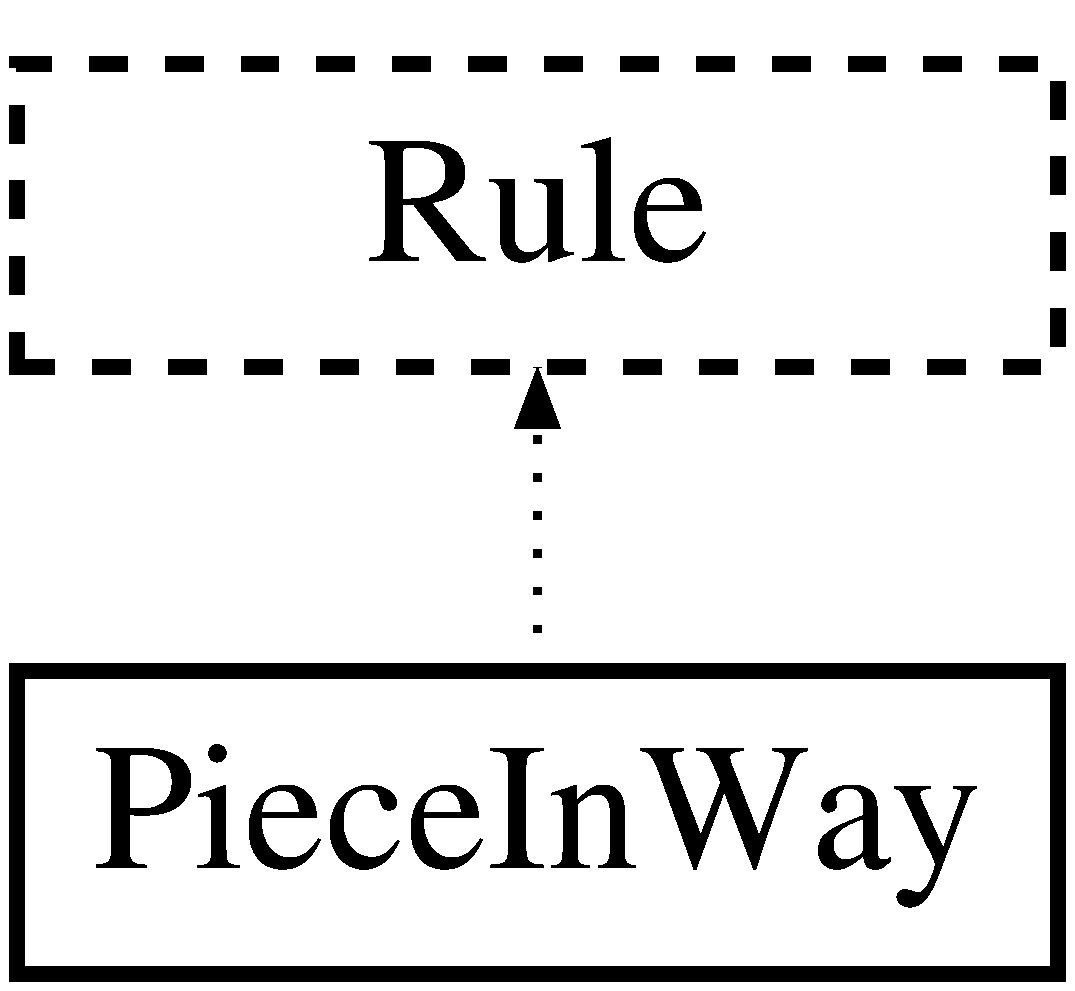
\includegraphics[height=2cm]{classPieceInWay}
\end{center}
\end{figure}
\subsection*{Public Member Functions}
\begin{DoxyCompactItemize}
\item 
\hyperlink{classPieceInWay_a9e3ba0268de2c0dde0d4ca047050020f}{PieceInWay} ()
\begin{DoxyCompactList}\small\item\em \hyperlink{classPieceInWay}{PieceInWay} creates a \hyperlink{classPieceInWay}{PieceInWay} object. \item\end{DoxyCompactList}\item 
int \hyperlink{classPieceInWay_a9b34a28e7b7b7ff310f5998ff5f49fb6}{validMove} (vector$<$ vector$<$ \hyperlink{classPiece}{Piece} $\ast$ $>$ $>$ \&b, int ix, int iy, int dx, int dy)
\begin{DoxyCompactList}\small\item\em validMove checks if there is any piece in between where the piece currently is and where it wants to move. if valid calls \hyperlink{classFriendlyPiece}{FriendlyPiece}. if invalid return 0. \item\end{DoxyCompactList}\end{DoxyCompactItemize}


\subsection{Constructor \& Destructor Documentation}
\hypertarget{classPieceInWay_a9e3ba0268de2c0dde0d4ca047050020f}{
\index{PieceInWay@{PieceInWay}!PieceInWay@{PieceInWay}}
\index{PieceInWay@{PieceInWay}!PieceInWay@{PieceInWay}}
\subsubsection[{PieceInWay}]{\setlength{\rightskip}{0pt plus 5cm}PieceInWay::PieceInWay ()}}
\label{classPieceInWay_a9e3ba0268de2c0dde0d4ca047050020f}


\hyperlink{classPieceInWay}{PieceInWay} creates a \hyperlink{classPieceInWay}{PieceInWay} object. 
\begin{DoxyParams}{Parameters}
\item[\mbox{$\leftarrow$} {\em b}]is a vector$<$ vector $<$ Piece$\ast$ $>$ $>$ object \item[\mbox{$\leftarrow$} {\em ix}]is the x for the initial location \item[\mbox{$\leftarrow$} {\em iy}]is the y for the initial location \item[\mbox{$\leftarrow$} {\em dx}]is the x for the destination location \item[\mbox{$\leftarrow$} {\em dy}]is the y for the destination location \end{DoxyParams}


\subsection{Member Function Documentation}
\hypertarget{classPieceInWay_a9b34a28e7b7b7ff310f5998ff5f49fb6}{
\index{PieceInWay@{PieceInWay}!validMove@{validMove}}
\index{validMove@{validMove}!PieceInWay@{PieceInWay}}
\subsubsection[{validMove}]{\setlength{\rightskip}{0pt plus 5cm}int PieceInWay::validMove (vector$<$ vector$<$ {\bf Piece} $\ast$ $>$ $>$ \& {\em b}, \/  int {\em ix}, \/  int {\em iy}, \/  int {\em dx}, \/  int {\em dy})\hspace{0.3cm}{\ttfamily  \mbox{[}virtual\mbox{]}}}}
\label{classPieceInWay_a9b34a28e7b7b7ff310f5998ff5f49fb6}


validMove checks if there is any piece in between where the piece currently is and where it wants to move. if valid calls \hyperlink{classFriendlyPiece}{FriendlyPiece}. if invalid return 0. \begin{DoxyReturn}{Returns}
an int 
\end{DoxyReturn}


Implements \hyperlink{classRule}{Rule}.

The documentation for this class was generated from the following files:\begin{DoxyCompactItemize}
\item 
source/Rules/\hyperlink{PieceInWay_8h}{PieceInWay.h}\item 
source/Rules/PieceInWay.cc\end{DoxyCompactItemize}

\hypertarget{classPlayer}{
\section{Player Class Reference}
\label{classPlayer}\index{Player@{Player}}
}
Inheritance diagram for Player::\begin{figure}[H]
\begin{center}
\leavevmode
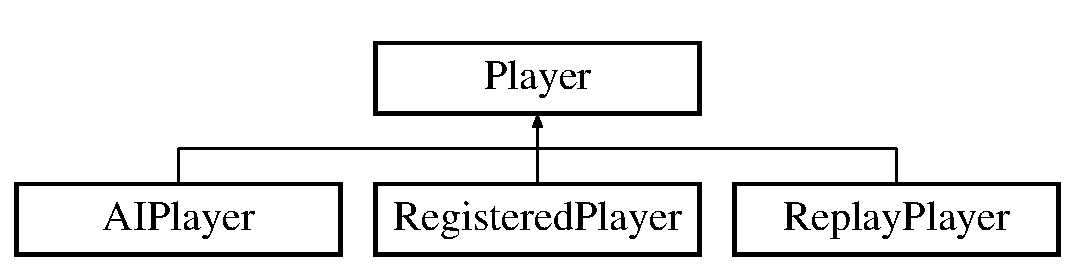
\includegraphics[height=2cm]{classPlayer}
\end{center}
\end{figure}
\subsection*{Public Member Functions}
\begin{DoxyCompactItemize}
\item 
\hypertarget{classPlayer_a9ca1e3c3a8ad5d89268551b93a19fcc0}{
virtual string {\bfseries getName} ()=0}
\label{classPlayer_a9ca1e3c3a8ad5d89268551b93a19fcc0}

\item 
virtual \hyperlink{classMemento}{Memento} $\ast$ \hyperlink{classPlayer_ae0b947230fe2f09d96f273798f19cf0d}{generateMemento} ()=0
\begin{DoxyCompactList}\small\item\em Generates a \hyperlink{classMemento}{Memento} object. \item\end{DoxyCompactList}\item 
virtual void \hyperlink{classPlayer_a9c4f1a1eef2fbfda4b6e19e97be91877}{restoreMemento} (\hyperlink{classMemento}{Memento} $\ast$memento)=0
\begin{DoxyCompactList}\small\item\em Restores this \hyperlink{classRegisteredPlayer}{RegisteredPlayer} object from the \hyperlink{classMemento}{Memento} object. \item\end{DoxyCompactList}\end{DoxyCompactItemize}


\subsection{Member Function Documentation}
\hypertarget{classPlayer_ae0b947230fe2f09d96f273798f19cf0d}{
\index{Player@{Player}!generateMemento@{generateMemento}}
\index{generateMemento@{generateMemento}!Player@{Player}}
\subsubsection[{generateMemento}]{\setlength{\rightskip}{0pt plus 5cm}virtual {\bf Memento}$\ast$ Player::generateMemento ()\hspace{0.3cm}{\ttfamily  \mbox{[}pure virtual\mbox{]}}}}
\label{classPlayer_ae0b947230fe2f09d96f273798f19cf0d}


Generates a \hyperlink{classMemento}{Memento} object. \begin{DoxyReturn}{Returns}
returns a memento object 
\end{DoxyReturn}


Implemented in \hyperlink{classAIPlayer_a83d0865c5869bbf02a66207976842de6}{AIPlayer}, \hyperlink{classRegisteredPlayer_ab9436dac85b13fe2ad6849eb4efb02b8}{RegisteredPlayer}, and \hyperlink{classReplayPlayer_a9301be927a78f52b14602f6660ce35c4}{ReplayPlayer}.\hypertarget{classPlayer_a9c4f1a1eef2fbfda4b6e19e97be91877}{
\index{Player@{Player}!restoreMemento@{restoreMemento}}
\index{restoreMemento@{restoreMemento}!Player@{Player}}
\subsubsection[{restoreMemento}]{\setlength{\rightskip}{0pt plus 5cm}virtual void Player::restoreMemento ({\bf Memento} $\ast$ {\em memento})\hspace{0.3cm}{\ttfamily  \mbox{[}pure virtual\mbox{]}}}}
\label{classPlayer_a9c4f1a1eef2fbfda4b6e19e97be91877}


Restores this \hyperlink{classRegisteredPlayer}{RegisteredPlayer} object from the \hyperlink{classMemento}{Memento} object. 
\begin{DoxyParams}{Parameters}
\item[\mbox{$\leftarrow$} {\em memento}]the memento object to restore \end{DoxyParams}


Implemented in \hyperlink{classRegisteredPlayer_a2a588dca8f68c5d72b4f73312f017c4d}{RegisteredPlayer}.

The documentation for this class was generated from the following file:\begin{DoxyCompactItemize}
\item 
source/Players/Player.h\end{DoxyCompactItemize}

\hypertarget{classPromotion}{
\section{Promotion Class Reference}
\label{classPromotion}\index{Promotion@{Promotion}}
}
Inheritance diagram for Promotion::\begin{figure}[H]
\begin{center}
\leavevmode
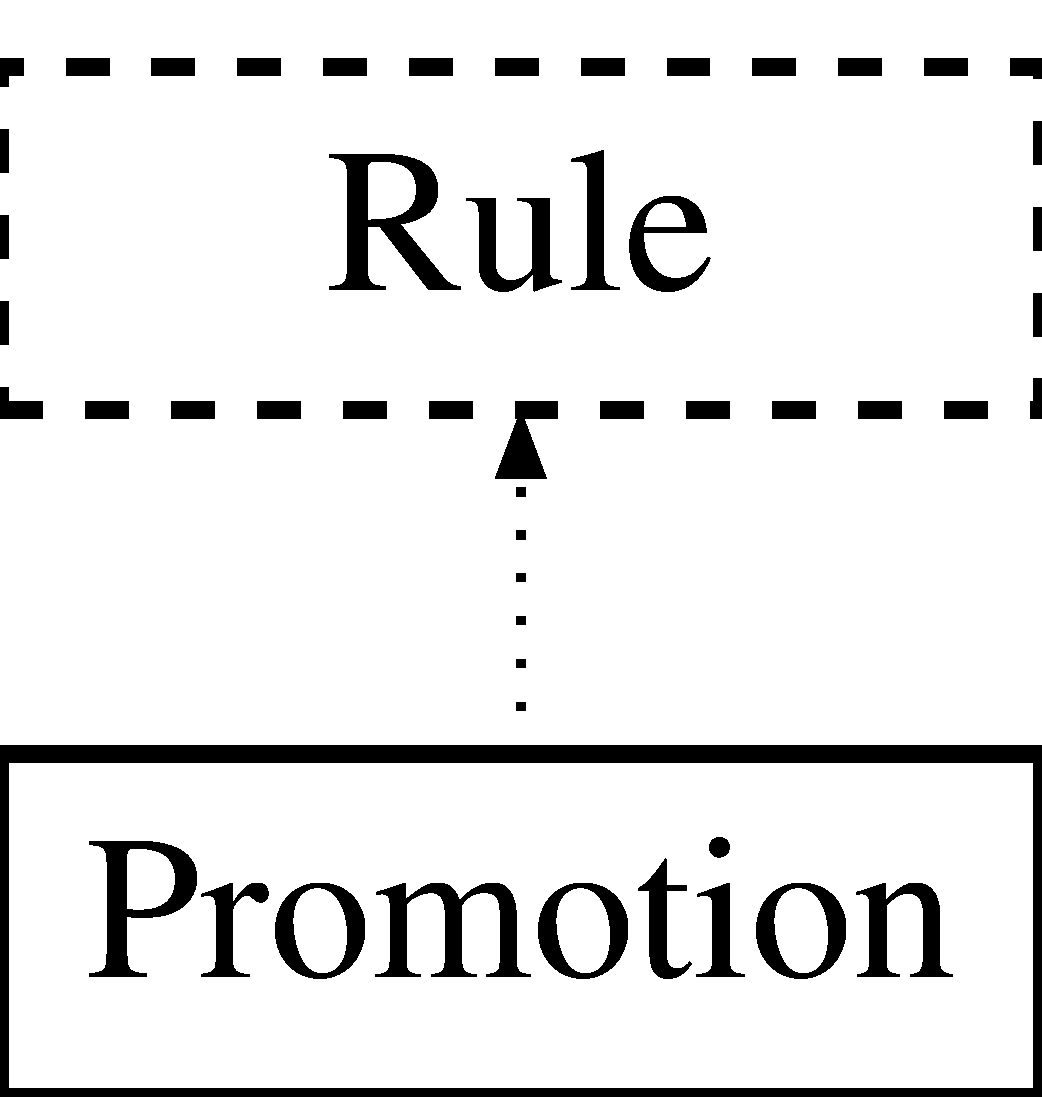
\includegraphics[height=2cm]{classPromotion}
\end{center}
\end{figure}
\subsection*{Public Member Functions}
\begin{DoxyCompactItemize}
\item 
\hyperlink{classPromotion_aa10833a0510fd7fdf3a8b7019ae61531}{Promotion} ()
\begin{DoxyCompactList}\small\item\em \hyperlink{classPromotion}{Promotion} creates a \hyperlink{classPromotion}{Promotion} object. \item\end{DoxyCompactList}\item 
int \hyperlink{classPromotion_abbf445a4b494712e0b8d8b6b3e69e0cf}{validMove} (vector$<$ vector$<$ \hyperlink{classPiece}{Piece} $\ast$ $>$ $>$ \&b, int ix, int iy, int dx, int dy)
\begin{DoxyCompactList}\small\item\em validMove if the location at where the pawn is requesting to move is at the end of the vector$<$ vector $<$ Piece$\ast$ $>$ $>$ return 3(so the pawn moves to that location and gets promoted) if the location at where the pawn requested to be is not at the end of the vector$<$ vector $<$ Piece$\ast$ $>$ $>$ then go to \hyperlink{classPieceInWay}{PieceInWay}. \item\end{DoxyCompactList}\end{DoxyCompactItemize}


\subsection{Constructor \& Destructor Documentation}
\hypertarget{classPromotion_aa10833a0510fd7fdf3a8b7019ae61531}{
\index{Promotion@{Promotion}!Promotion@{Promotion}}
\index{Promotion@{Promotion}!Promotion@{Promotion}}
\subsubsection[{Promotion}]{\setlength{\rightskip}{0pt plus 5cm}Promotion::Promotion ()}}
\label{classPromotion_aa10833a0510fd7fdf3a8b7019ae61531}


\hyperlink{classPromotion}{Promotion} creates a \hyperlink{classPromotion}{Promotion} object. 
\begin{DoxyParams}{Parameters}
\item[\mbox{$\leftarrow$} {\em b}]is a vector$<$ vector $<$ Piece$\ast$ $>$ $>$ object \item[\mbox{$\leftarrow$} {\em ix}]is the x for the initial location \item[\mbox{$\leftarrow$} {\em iy}]is the y for the initial location \item[\mbox{$\leftarrow$} {\em dx}]is the x for the destination location \item[\mbox{$\leftarrow$} {\em dy}]is the y for the destination location \end{DoxyParams}


\subsection{Member Function Documentation}
\hypertarget{classPromotion_abbf445a4b494712e0b8d8b6b3e69e0cf}{
\index{Promotion@{Promotion}!validMove@{validMove}}
\index{validMove@{validMove}!Promotion@{Promotion}}
\subsubsection[{validMove}]{\setlength{\rightskip}{0pt plus 5cm}int Promotion::validMove (vector$<$ vector$<$ {\bf Piece} $\ast$ $>$ $>$ \& {\em b}, \/  int {\em ix}, \/  int {\em iy}, \/  int {\em dx}, \/  int {\em dy})\hspace{0.3cm}{\ttfamily  \mbox{[}virtual\mbox{]}}}}
\label{classPromotion_abbf445a4b494712e0b8d8b6b3e69e0cf}


validMove if the location at where the pawn is requesting to move is at the end of the vector$<$ vector $<$ Piece$\ast$ $>$ $>$ return 3(so the pawn moves to that location and gets promoted) if the location at where the pawn requested to be is not at the end of the vector$<$ vector $<$ Piece$\ast$ $>$ $>$ then go to \hyperlink{classPieceInWay}{PieceInWay}. \begin{DoxyReturn}{Returns}
an int 
\end{DoxyReturn}


Implements \hyperlink{classRule}{Rule}.

The documentation for this class was generated from the following files:\begin{DoxyCompactItemize}
\item 
source/Rules/\hyperlink{Promotion_8h}{Promotion.h}\item 
source/Rules/Promotion.cc\end{DoxyCompactItemize}

\hypertarget{classQueenMove}{
\section{QueenMove Class Reference}
\label{classQueenMove}\index{QueenMove@{QueenMove}}
}
Inheritance diagram for QueenMove::\begin{figure}[H]
\begin{center}
\leavevmode
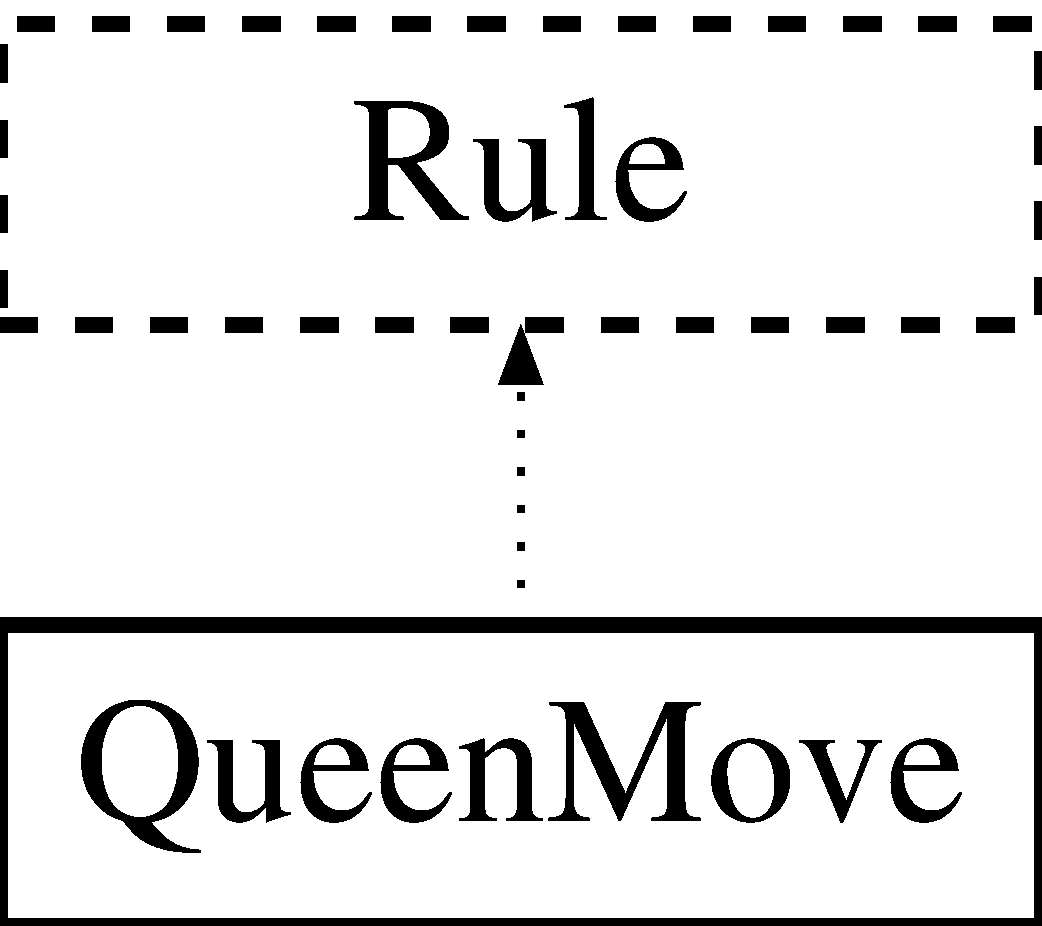
\includegraphics[height=2cm]{classQueenMove}
\end{center}
\end{figure}
\subsection*{Public Member Functions}
\begin{DoxyCompactItemize}
\item 
\hyperlink{classQueenMove_a62bbd2eb2e49ba93b7144403cfc8eb46}{QueenMove} ()
\begin{DoxyCompactList}\small\item\em \hyperlink{classQueenMove}{QueenMove} creates a \hyperlink{classQueenMove}{QueenMove} object. \item\end{DoxyCompactList}\item 
int \hyperlink{classQueenMove_a20dad2546b24626a9c00e5c3b3369065}{validMove} (vector$<$ vector$<$ \hyperlink{classPiece}{Piece} $\ast$ $>$ $>$ \&b, int ix, int iy, int dx, int dy)
\begin{DoxyCompactList}\small\item\em validMove if the queens requested location is either on the x axis or on the y axis, or if it is a on a perfect angle(ex. x+1, y+1) if any are true go to \hyperlink{classPieceInWay}{PieceInWay}, else return 0. \item\end{DoxyCompactList}\end{DoxyCompactItemize}


\subsection{Constructor \& Destructor Documentation}
\hypertarget{classQueenMove_a62bbd2eb2e49ba93b7144403cfc8eb46}{
\index{QueenMove@{QueenMove}!QueenMove@{QueenMove}}
\index{QueenMove@{QueenMove}!QueenMove@{QueenMove}}
\subsubsection[{QueenMove}]{\setlength{\rightskip}{0pt plus 5cm}QueenMove::QueenMove ()}}
\label{classQueenMove_a62bbd2eb2e49ba93b7144403cfc8eb46}


\hyperlink{classQueenMove}{QueenMove} creates a \hyperlink{classQueenMove}{QueenMove} object. 
\begin{DoxyParams}{Parameters}
\item[\mbox{$\leftarrow$} {\em b}]is a vector$<$ vector $<$ Piece$\ast$ $>$ $>$ object \item[\mbox{$\leftarrow$} {\em ix}]is the x for the initial location \item[\mbox{$\leftarrow$} {\em iy}]is the y for the initial location \item[\mbox{$\leftarrow$} {\em dx}]is the x for the destination location \item[\mbox{$\leftarrow$} {\em dy}]is the y for the destination location \end{DoxyParams}


\subsection{Member Function Documentation}
\hypertarget{classQueenMove_a20dad2546b24626a9c00e5c3b3369065}{
\index{QueenMove@{QueenMove}!validMove@{validMove}}
\index{validMove@{validMove}!QueenMove@{QueenMove}}
\subsubsection[{validMove}]{\setlength{\rightskip}{0pt plus 5cm}int QueenMove::validMove (vector$<$ vector$<$ {\bf Piece} $\ast$ $>$ $>$ \& {\em b}, \/  int {\em ix}, \/  int {\em iy}, \/  int {\em dx}, \/  int {\em dy})\hspace{0.3cm}{\ttfamily  \mbox{[}virtual\mbox{]}}}}
\label{classQueenMove_a20dad2546b24626a9c00e5c3b3369065}


validMove if the queens requested location is either on the x axis or on the y axis, or if it is a on a perfect angle(ex. x+1, y+1) if any are true go to \hyperlink{classPieceInWay}{PieceInWay}, else return 0. \begin{DoxyReturn}{Returns}
an int 
\end{DoxyReturn}


Implements \hyperlink{classRule}{Rule}.

The documentation for this class was generated from the following files:\begin{DoxyCompactItemize}
\item 
source/Rules/\hyperlink{QueenMove_8h}{QueenMove.h}\item 
source/Rules/QueenMove.cc\end{DoxyCompactItemize}

\hypertarget{classQueenPiece}{
\section{QueenPiece Class Reference}
\label{classQueenPiece}\index{QueenPiece@{QueenPiece}}
}


a class for all Queen Piece`s.  


{\ttfamily \#include $<$QueenPiece.h$>$}Inheritance diagram for QueenPiece::\begin{figure}[H]
\begin{center}
\leavevmode
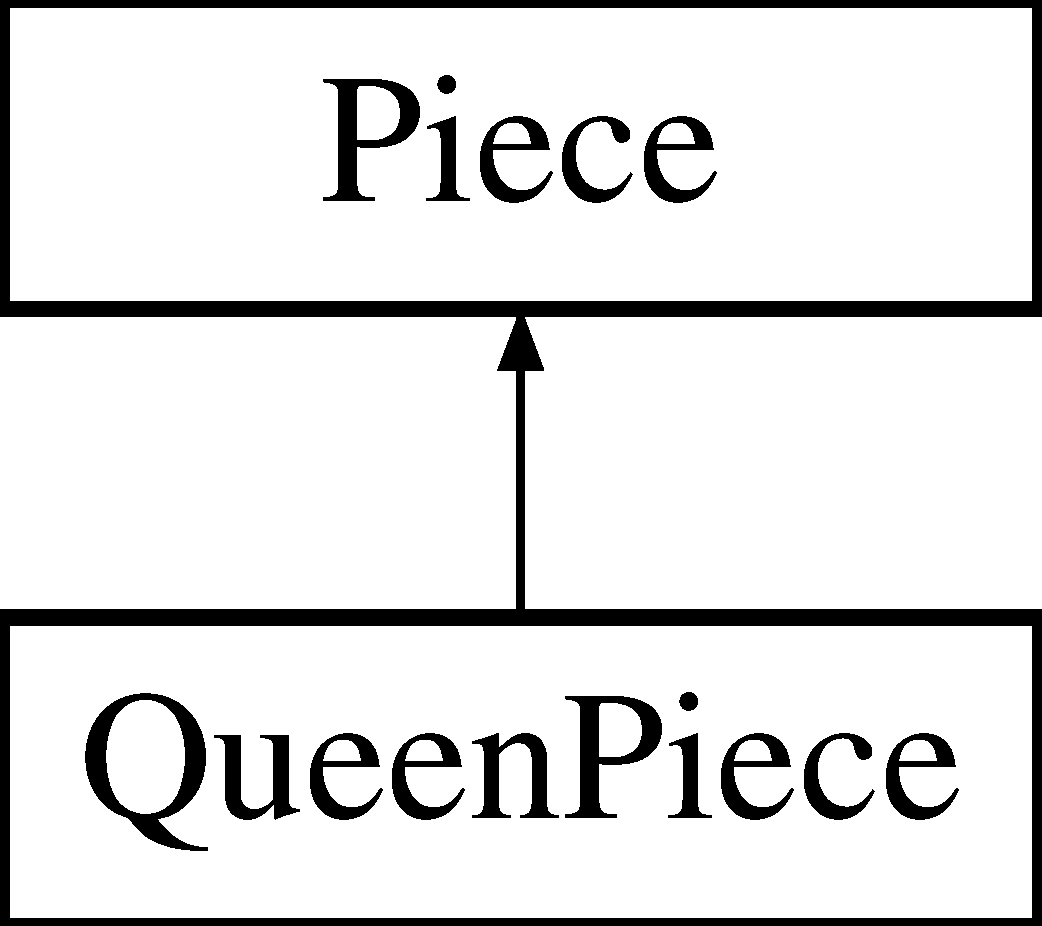
\includegraphics[height=2cm]{classQueenPiece}
\end{center}
\end{figure}
\subsection*{Public Member Functions}
\begin{DoxyCompactItemize}
\item 
\hypertarget{classQueenPiece_a0eca088526b0b1a2648575fe867b3a9b}{
\hyperlink{classQueenPiece_a0eca088526b0b1a2648575fe867b3a9b}{QueenPiece} (int c=0)}
\label{classQueenPiece_a0eca088526b0b1a2648575fe867b3a9b}

\begin{DoxyCompactList}\small\item\em creates a \hyperlink{classPiece}{Piece} object \item\end{DoxyCompactList}\item 
int \hyperlink{classQueenPiece_a461d58f951b5e9f4d120cec0c47a1d9c}{getColor} () const 
\begin{DoxyCompactList}\small\item\em gets the color of the Queen \hyperlink{classPiece}{Piece} \item\end{DoxyCompactList}\item 
void \hyperlink{classQueenPiece_a691ff6afc7d167dab9cff0c910cae859}{setColor} (int colorOfPiece)
\begin{DoxyCompactList}\small\item\em sets the Color of the Queen \hyperlink{classPiece}{Piece} \item\end{DoxyCompactList}\item 
string \hyperlink{classQueenPiece_ae8df61c033b58d7f96e344166a9f2bdb}{getType} () const 
\begin{DoxyCompactList}\small\item\em Returns Queen to user. \item\end{DoxyCompactList}\item 
int \hyperlink{classQueenPiece_a5db59b743df799adc37ce6a3c0230458}{validMove} (vector$<$ vector$<$ \hyperlink{classPiece}{Piece} $\ast$ $>$ $>$ gameBoard, int ix, int iy, int dx, int dy)
\begin{DoxyCompactList}\small\item\em validates a move based on the Queen rules. \item\end{DoxyCompactList}\end{DoxyCompactItemize}


\subsection{Detailed Description}
a class for all Queen Piece`s. 

\subsection{Member Function Documentation}
\hypertarget{classQueenPiece_a461d58f951b5e9f4d120cec0c47a1d9c}{
\index{QueenPiece@{QueenPiece}!getColor@{getColor}}
\index{getColor@{getColor}!QueenPiece@{QueenPiece}}
\subsubsection[{getColor}]{\setlength{\rightskip}{0pt plus 5cm}int QueenPiece::getColor () const\hspace{0.3cm}{\ttfamily  \mbox{[}virtual\mbox{]}}}}
\label{classQueenPiece_a461d58f951b5e9f4d120cec0c47a1d9c}


gets the color of the Queen \hyperlink{classPiece}{Piece} \begin{DoxyReturn}{Returns}
int a 0 if white and 1 if black 
\end{DoxyReturn}


Implements \hyperlink{classPiece_a1376072d4815719e60253ce5688df95c}{Piece}.\hypertarget{classQueenPiece_ae8df61c033b58d7f96e344166a9f2bdb}{
\index{QueenPiece@{QueenPiece}!getType@{getType}}
\index{getType@{getType}!QueenPiece@{QueenPiece}}
\subsubsection[{getType}]{\setlength{\rightskip}{0pt plus 5cm}string QueenPiece::getType () const\hspace{0.3cm}{\ttfamily  \mbox{[}virtual\mbox{]}}}}
\label{classQueenPiece_ae8df61c033b58d7f96e344166a9f2bdb}


Returns Queen to user. \begin{DoxyReturn}{Returns}
a string that will return Queen Type. 
\end{DoxyReturn}


Implements \hyperlink{classPiece_a5b88fcd786bb30b345b24fbc3ab24ab9}{Piece}.\hypertarget{classQueenPiece_a691ff6afc7d167dab9cff0c910cae859}{
\index{QueenPiece@{QueenPiece}!setColor@{setColor}}
\index{setColor@{setColor}!QueenPiece@{QueenPiece}}
\subsubsection[{setColor}]{\setlength{\rightskip}{0pt plus 5cm}void QueenPiece::setColor (int {\em colorOfPiece})\hspace{0.3cm}{\ttfamily  \mbox{[}virtual\mbox{]}}}}
\label{classQueenPiece_a691ff6afc7d167dab9cff0c910cae859}


sets the Color of the Queen \hyperlink{classPiece}{Piece} 
\begin{DoxyParams}{Parameters}
\item[\mbox{$\leftarrow$} {\em colorOfPiece}]sets the Queen Piece`s color \end{DoxyParams}


Implements \hyperlink{classPiece_a1387cb503dca308ac1e3bbe38a70a073}{Piece}.\hypertarget{classQueenPiece_a5db59b743df799adc37ce6a3c0230458}{
\index{QueenPiece@{QueenPiece}!validMove@{validMove}}
\index{validMove@{validMove}!QueenPiece@{QueenPiece}}
\subsubsection[{validMove}]{\setlength{\rightskip}{0pt plus 5cm}int QueenPiece::validMove (vector$<$ vector$<$ {\bf Piece} $\ast$ $>$ $>$ {\em gameBoard}, \/  int {\em ix}, \/  int {\em iy}, \/  int {\em dx}, \/  int {\em dy})}}
\label{classQueenPiece_a5db59b743df799adc37ce6a3c0230458}


validates a move based on the Queen rules. 
\begin{DoxyParams}{Parameters}
\item[\mbox{$\leftarrow$} {\em board}]A \hyperlink{classBoard}{Board} that will contain the currect board state \item[\mbox{$\leftarrow$} {\em ix}]A int that holds the x coordinate of where the piece is moving from \item[\mbox{$\leftarrow$} {\em iy}]A int that holds the y coordinate of where the piece is moving from \item[\mbox{$\leftarrow$} {\em dx}]A int that holds the x coordinate of where the piece is moving to \item[\mbox{$\leftarrow$} {\em dy}]A int that holds the y coordinate of where the piece is moving to \end{DoxyParams}


The documentation for this class was generated from the following files:\begin{DoxyCompactItemize}
\item 
source/Piece/\hyperlink{QueenPiece_8h}{QueenPiece.h}\item 
source/Piece/QueenPiece.cc\end{DoxyCompactItemize}

\hypertarget{classRegisteredPlayer}{
\section{RegisteredPlayer Class Reference}
\label{classRegisteredPlayer}\index{RegisteredPlayer@{RegisteredPlayer}}
}
Inheritance diagram for RegisteredPlayer::\begin{figure}[H]
\begin{center}
\leavevmode
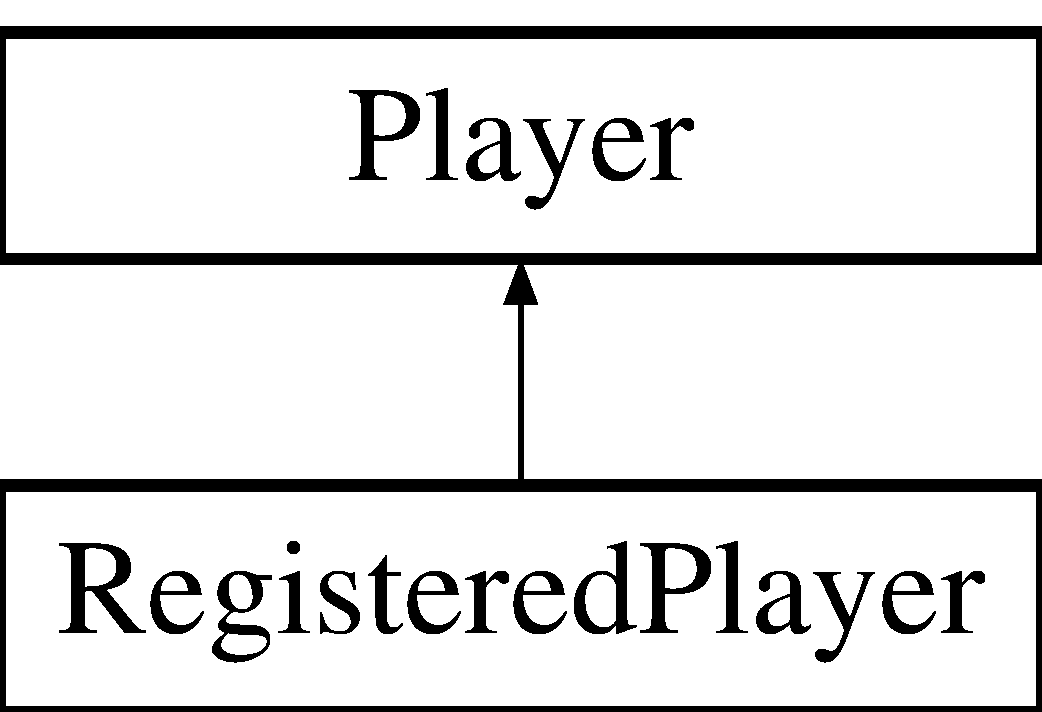
\includegraphics[height=2cm]{classRegisteredPlayer}
\end{center}
\end{figure}
\subsection*{Public Member Functions}
\begin{DoxyCompactItemize}
\item 
\hypertarget{classRegisteredPlayer_a456be7066169306026a0d7d359d74799}{
\hyperlink{classRegisteredPlayer_a456be7066169306026a0d7d359d74799}{RegisteredPlayer} (string name=\char`\"{}Guest\char`\"{})}
\label{classRegisteredPlayer_a456be7066169306026a0d7d359d74799}

\begin{DoxyCompactList}\small\item\em creates a \hyperlink{classRegisteredPlayer}{RegisteredPlayer} from the data base \item\end{DoxyCompactList}\item 
\hypertarget{classRegisteredPlayer_a9cc8da7f1f03440e38e5bfddd90c448c}{
\hyperlink{classRegisteredPlayer_a9cc8da7f1f03440e38e5bfddd90c448c}{$\sim$RegisteredPlayer} ()}
\label{classRegisteredPlayer_a9cc8da7f1f03440e38e5bfddd90c448c}

\begin{DoxyCompactList}\small\item\em destructor for \hyperlink{classRegisteredPlayer}{RegisteredPlayer} \item\end{DoxyCompactList}\item 
bool \hyperlink{classRegisteredPlayer_aae6a64176b51f7e7b3b1ef745c9f1119}{setElo} ()
\item 
\hypertarget{classRegisteredPlayer_ae4c5461f0f7444025402a23a590b491b}{
int \hyperlink{classRegisteredPlayer_ae4c5461f0f7444025402a23a590b491b}{getElo} ()}
\label{classRegisteredPlayer_ae4c5461f0f7444025402a23a590b491b}

\begin{DoxyCompactList}\small\item\em returns the ELO \item\end{DoxyCompactList}\item 
\hypertarget{classRegisteredPlayer_a6f2c3d36cfe1451955a48c10e07f27d6}{
int \hyperlink{classRegisteredPlayer_a6f2c3d36cfe1451955a48c10e07f27d6}{getGamesWon} ()}
\label{classRegisteredPlayer_a6f2c3d36cfe1451955a48c10e07f27d6}

\begin{DoxyCompactList}\small\item\em returns the Games won \item\end{DoxyCompactList}\item 
\hypertarget{classRegisteredPlayer_a7511d11c93e2571b776f332154256e53}{
bool \hyperlink{classRegisteredPlayer_a7511d11c93e2571b776f332154256e53}{incrementGamesWon} ()}
\label{classRegisteredPlayer_a7511d11c93e2571b776f332154256e53}

\begin{DoxyCompactList}\small\item\em returns a bool based on whether games won has been sucessfully updated \item\end{DoxyCompactList}\item 
\hypertarget{classRegisteredPlayer_ad36ab2a8410ab7c1737f4e6a42dd700e}{
int \hyperlink{classRegisteredPlayer_ad36ab2a8410ab7c1737f4e6a42dd700e}{getGamesLost} ()}
\label{classRegisteredPlayer_ad36ab2a8410ab7c1737f4e6a42dd700e}

\begin{DoxyCompactList}\small\item\em returns the Games won \item\end{DoxyCompactList}\item 
\hypertarget{classRegisteredPlayer_a2ee5bcbc942517c3d22475f96c9937c9}{
bool \hyperlink{classRegisteredPlayer_a2ee5bcbc942517c3d22475f96c9937c9}{incrementGamesLost} ()}
\label{classRegisteredPlayer_a2ee5bcbc942517c3d22475f96c9937c9}

\begin{DoxyCompactList}\small\item\em returns a bool based on whether games lost has been sucessfully updated \item\end{DoxyCompactList}\item 
\hypertarget{classRegisteredPlayer_ababd7f33044952a9e16697ec13f74c40}{
string \hyperlink{classRegisteredPlayer_ababd7f33044952a9e16697ec13f74c40}{getName} ()}
\label{classRegisteredPlayer_ababd7f33044952a9e16697ec13f74c40}

\begin{DoxyCompactList}\small\item\em returns the name of this player \item\end{DoxyCompactList}\item 
\hyperlink{classMemento}{Memento} $\ast$ \hyperlink{classRegisteredPlayer_ab9436dac85b13fe2ad6849eb4efb02b8}{generateMemento} ()
\begin{DoxyCompactList}\small\item\em Generates a \hyperlink{classMemento}{Memento} object. \item\end{DoxyCompactList}\item 
void \hyperlink{classRegisteredPlayer_a2a588dca8f68c5d72b4f73312f017c4d}{restoreMemento} (\hyperlink{classMemento}{Memento} $\ast$memento)
\begin{DoxyCompactList}\small\item\em Restores this \hyperlink{classRegisteredPlayer}{RegisteredPlayer} object from the \hyperlink{classMemento}{Memento} object. \item\end{DoxyCompactList}\end{DoxyCompactItemize}


\subsection{Member Function Documentation}
\hypertarget{classRegisteredPlayer_ab9436dac85b13fe2ad6849eb4efb02b8}{
\index{RegisteredPlayer@{RegisteredPlayer}!generateMemento@{generateMemento}}
\index{generateMemento@{generateMemento}!RegisteredPlayer@{RegisteredPlayer}}
\subsubsection[{generateMemento}]{\setlength{\rightskip}{0pt plus 5cm}{\bf Memento} $\ast$ RegisteredPlayer::generateMemento ()\hspace{0.3cm}{\ttfamily  \mbox{[}virtual\mbox{]}}}}
\label{classRegisteredPlayer_ab9436dac85b13fe2ad6849eb4efb02b8}


Generates a \hyperlink{classMemento}{Memento} object. \begin{DoxyReturn}{Returns}
returns a memento object 
\end{DoxyReturn}


Implements \hyperlink{classPlayer_ae0b947230fe2f09d96f273798f19cf0d}{Player}.\hypertarget{classRegisteredPlayer_a2a588dca8f68c5d72b4f73312f017c4d}{
\index{RegisteredPlayer@{RegisteredPlayer}!restoreMemento@{restoreMemento}}
\index{restoreMemento@{restoreMemento}!RegisteredPlayer@{RegisteredPlayer}}
\subsubsection[{restoreMemento}]{\setlength{\rightskip}{0pt plus 5cm}void RegisteredPlayer::restoreMemento ({\bf Memento} $\ast$ {\em memento})\hspace{0.3cm}{\ttfamily  \mbox{[}virtual\mbox{]}}}}
\label{classRegisteredPlayer_a2a588dca8f68c5d72b4f73312f017c4d}


Restores this \hyperlink{classRegisteredPlayer}{RegisteredPlayer} object from the \hyperlink{classMemento}{Memento} object. 
\begin{DoxyParams}{Parameters}
\item[\mbox{$\leftarrow$} {\em memento}]the memento object to restore \end{DoxyParams}


Implements \hyperlink{classPlayer_a9c4f1a1eef2fbfda4b6e19e97be91877}{Player}.\hypertarget{classRegisteredPlayer_aae6a64176b51f7e7b3b1ef745c9f1119}{
\index{RegisteredPlayer@{RegisteredPlayer}!setElo@{setElo}}
\index{setElo@{setElo}!RegisteredPlayer@{RegisteredPlayer}}
\subsubsection[{setElo}]{\setlength{\rightskip}{0pt plus 5cm}bool RegisteredPlayer::setElo ()}}
\label{classRegisteredPlayer_aae6a64176b51f7e7b3b1ef745c9f1119}
returns a bool based on whether ELO has been sucessfully updated The elo has been updated based on the end game score and if the player won 

The documentation for this class was generated from the following files:\begin{DoxyCompactItemize}
\item 
source/Players/RegisteredPlayer.h\item 
source/Players/RegisteredPlayer.cc\end{DoxyCompactItemize}

\hypertarget{classReplayPlayer}{
\section{ReplayPlayer Class Reference}
\label{classReplayPlayer}\index{ReplayPlayer@{ReplayPlayer}}
}


a class for ReplayPlayers  


{\ttfamily \#include $<$ReplayPlayer.h$>$}Inheritance diagram for ReplayPlayer::\begin{figure}[H]
\begin{center}
\leavevmode
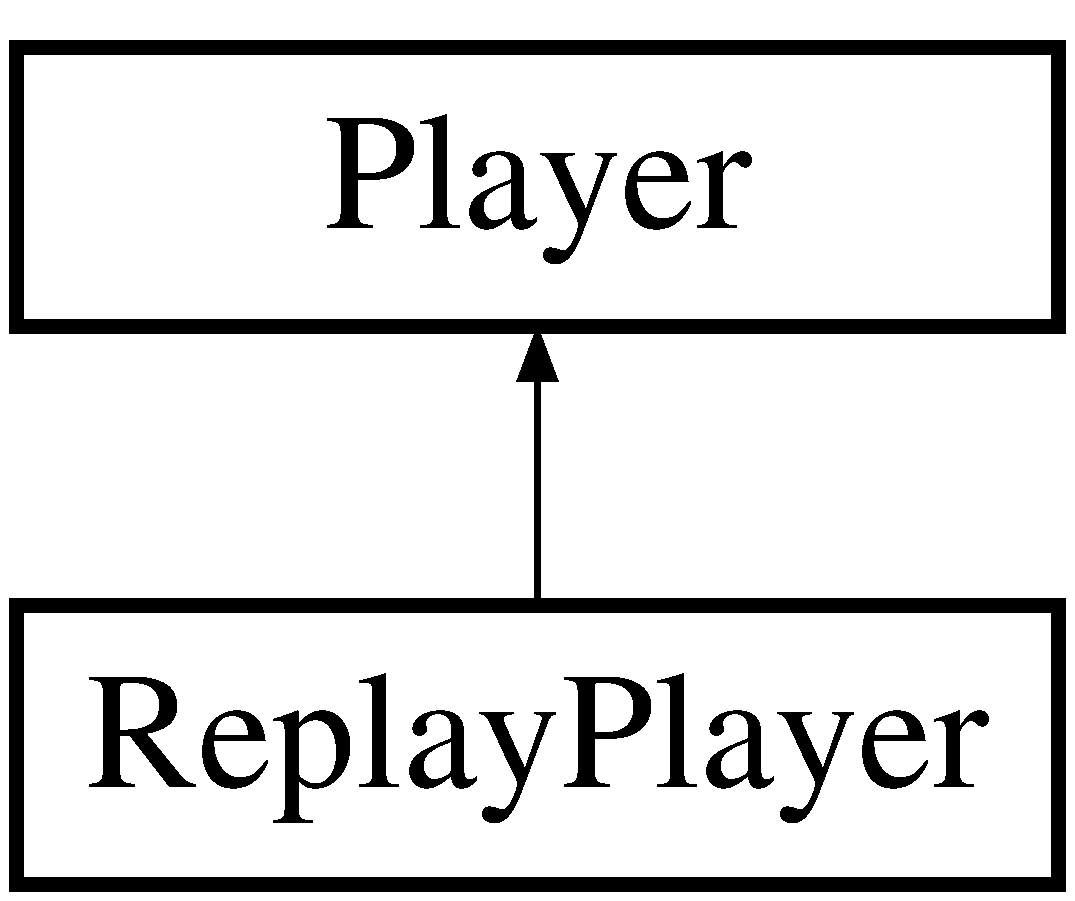
\includegraphics[height=2cm]{classReplayPlayer}
\end{center}
\end{figure}
\subsection*{Public Member Functions}
\begin{DoxyCompactItemize}
\item 
\hyperlink{classReplayPlayer_a39c2542b03506ff19487dc8675741298}{nextMove} (\hyperlink{classPiece}{Piece} p)
\begin{DoxyCompactList}\small\item\em creates a \hyperlink{classPlayer}{Player} \item\end{DoxyCompactList}\item 
\hyperlink{classMemento}{Memento} \hyperlink{classReplayPlayer_a9301be927a78f52b14602f6660ce35c4}{generateMemento} ()
\begin{DoxyCompactList}\small\item\em Generates a \hyperlink{classMemento}{Memento} object. \item\end{DoxyCompactList}\item 
void \hyperlink{classReplayPlayer_af45543802dc6f5ac1f7d8f2582c7a04e}{restoreMemento} (\hyperlink{classMemento}{Memento} memento)
\begin{DoxyCompactList}\small\item\em Restores this \hyperlink{classRegisteredPlayer}{RegisteredPlayer} object from the \hyperlink{classMemento}{Memento} object. \item\end{DoxyCompactList}\end{DoxyCompactItemize}


\subsection{Detailed Description}
a class for ReplayPlayers .h \begin{DoxyAuthor}{Author}
Zackery Shortt 
\end{DoxyAuthor}
\begin{DoxyDate}{Date}
October 27, 2014 
\end{DoxyDate}


\subsection{Member Function Documentation}
\hypertarget{classReplayPlayer_a9301be927a78f52b14602f6660ce35c4}{
\index{ReplayPlayer@{ReplayPlayer}!generateMemento@{generateMemento}}
\index{generateMemento@{generateMemento}!ReplayPlayer@{ReplayPlayer}}
\subsubsection[{generateMemento}]{\setlength{\rightskip}{0pt plus 5cm}{\bf Memento} ReplayPlayer::generateMemento ()\hspace{0.3cm}{\ttfamily  \mbox{[}virtual\mbox{]}}}}
\label{classReplayPlayer_a9301be927a78f52b14602f6660ce35c4}


Generates a \hyperlink{classMemento}{Memento} object. \begin{DoxyReturn}{Returns}
returns a memento object 
\end{DoxyReturn}


Implements \hyperlink{classPlayer_ae0b947230fe2f09d96f273798f19cf0d}{Player}.\hypertarget{classReplayPlayer_a39c2542b03506ff19487dc8675741298}{
\index{ReplayPlayer@{ReplayPlayer}!nextMove@{nextMove}}
\index{nextMove@{nextMove}!ReplayPlayer@{ReplayPlayer}}
\subsubsection[{nextMove}]{\setlength{\rightskip}{0pt plus 5cm}ReplayPlayer::nextMove ({\bf Piece} {\em p})}}
\label{classReplayPlayer_a39c2542b03506ff19487dc8675741298}


creates a \hyperlink{classPlayer}{Player} 
\begin{DoxyParams}{Parameters}
\item[\mbox{$\leftarrow$} {\em This}]is the \hyperlink{classPiece}{Piece} that will be moved \end{DoxyParams}
\hypertarget{classReplayPlayer_af45543802dc6f5ac1f7d8f2582c7a04e}{
\index{ReplayPlayer@{ReplayPlayer}!restoreMemento@{restoreMemento}}
\index{restoreMemento@{restoreMemento}!ReplayPlayer@{ReplayPlayer}}
\subsubsection[{restoreMemento}]{\setlength{\rightskip}{0pt plus 5cm}void ReplayPlayer::restoreMemento ({\bf Memento} {\em memento})}}
\label{classReplayPlayer_af45543802dc6f5ac1f7d8f2582c7a04e}


Restores this \hyperlink{classRegisteredPlayer}{RegisteredPlayer} object from the \hyperlink{classMemento}{Memento} object. 
\begin{DoxyParams}{Parameters}
\item[\mbox{$\leftarrow$} {\em memento}]the memento object to restore \end{DoxyParams}


The documentation for this class was generated from the following file:\begin{DoxyCompactItemize}
\item 
source/Players/ReplayPlayer.h\end{DoxyCompactItemize}

\hypertarget{classRookMove}{
\section{RookMove Class Reference}
\label{classRookMove}\index{RookMove@{RookMove}}
}
Inheritance diagram for RookMove::\begin{figure}[H]
\begin{center}
\leavevmode
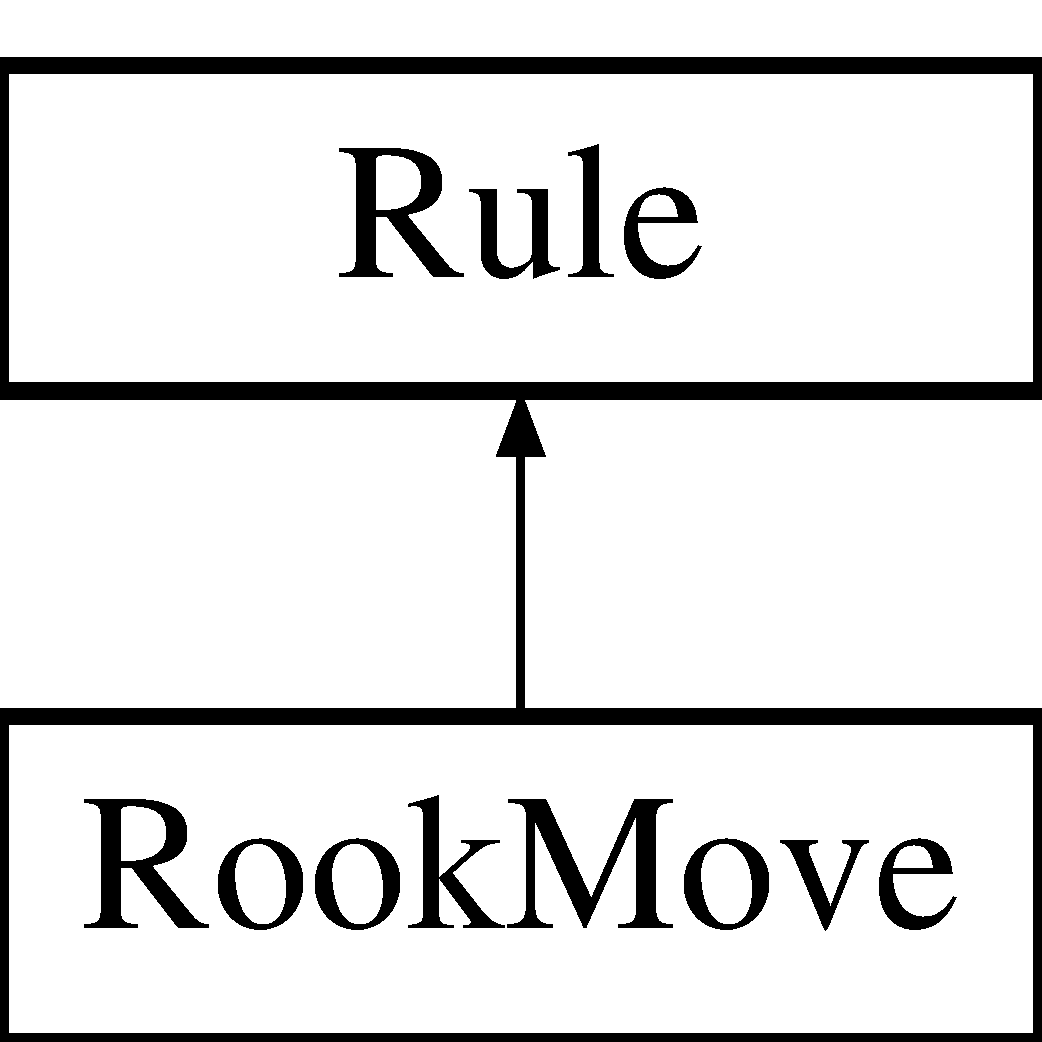
\includegraphics[height=2cm]{classRookMove}
\end{center}
\end{figure}
\subsection*{Public Member Functions}
\begin{DoxyCompactItemize}
\item 
\hyperlink{classRookMove_a74a07da059bd2a7dd2a8a644500efe8c}{RookMove} ()
\begin{DoxyCompactList}\small\item\em \hyperlink{classRookMove}{RookMove} creates a \hyperlink{classRookMove}{RookMove} object. \item\end{DoxyCompactList}\item 
int \hyperlink{classRookMove_a3b985caef5be53996c71ff3427816b68}{validMove} (vector$<$ vector$<$ \hyperlink{classPiece}{Piece} $\ast$ $>$ $>$ \&b, int ix, int iy, int dx, int dy)
\begin{DoxyCompactList}\small\item\em validMove if the rook requested location is either going strictly on the x axis or strictly on the y axis then go to \hyperlink{classPieceInWay}{PieceInWay} else return 0. \item\end{DoxyCompactList}\end{DoxyCompactItemize}


\subsection{Constructor \& Destructor Documentation}
\hypertarget{classRookMove_a74a07da059bd2a7dd2a8a644500efe8c}{
\index{RookMove@{RookMove}!RookMove@{RookMove}}
\index{RookMove@{RookMove}!RookMove@{RookMove}}
\subsubsection[{RookMove}]{\setlength{\rightskip}{0pt plus 5cm}RookMove::RookMove ()}}
\label{classRookMove_a74a07da059bd2a7dd2a8a644500efe8c}


\hyperlink{classRookMove}{RookMove} creates a \hyperlink{classRookMove}{RookMove} object. 
\begin{DoxyParams}{Parameters}
\item[\mbox{$\leftarrow$} {\em b}]is a vector$<$ vector $<$ Piece$\ast$ $>$ $>$ object \item[\mbox{$\leftarrow$} {\em ix}]is the x for the initial location \item[\mbox{$\leftarrow$} {\em iy}]is the y for the initial location \item[\mbox{$\leftarrow$} {\em dx}]is the x for the destination location \item[\mbox{$\leftarrow$} {\em dy}]is the y for the destination location \end{DoxyParams}


\subsection{Member Function Documentation}
\hypertarget{classRookMove_a3b985caef5be53996c71ff3427816b68}{
\index{RookMove@{RookMove}!validMove@{validMove}}
\index{validMove@{validMove}!RookMove@{RookMove}}
\subsubsection[{validMove}]{\setlength{\rightskip}{0pt plus 5cm}int RookMove::validMove (vector$<$ vector$<$ {\bf Piece} $\ast$ $>$ $>$ \& {\em b}, \/  int {\em ix}, \/  int {\em iy}, \/  int {\em dx}, \/  int {\em dy})\hspace{0.3cm}{\ttfamily  \mbox{[}virtual\mbox{]}}}}
\label{classRookMove_a3b985caef5be53996c71ff3427816b68}


validMove if the rook requested location is either going strictly on the x axis or strictly on the y axis then go to \hyperlink{classPieceInWay}{PieceInWay} else return 0. \begin{DoxyReturn}{Returns}
an int 
\end{DoxyReturn}


Implements \hyperlink{classRule}{Rule}.

The documentation for this class was generated from the following files:\begin{DoxyCompactItemize}
\item 
source/Rules/\hyperlink{RookMove_8h}{RookMove.h}\item 
source/Rules/RookMove.cc\end{DoxyCompactItemize}

\hypertarget{classRookPiece}{
\section{RookPiece Class Reference}
\label{classRookPiece}\index{RookPiece@{RookPiece}}
}


a class for all Rook Piece`s.  


{\ttfamily \#include $<$RookPiece.h$>$}Inheritance diagram for RookPiece::\begin{figure}[H]
\begin{center}
\leavevmode
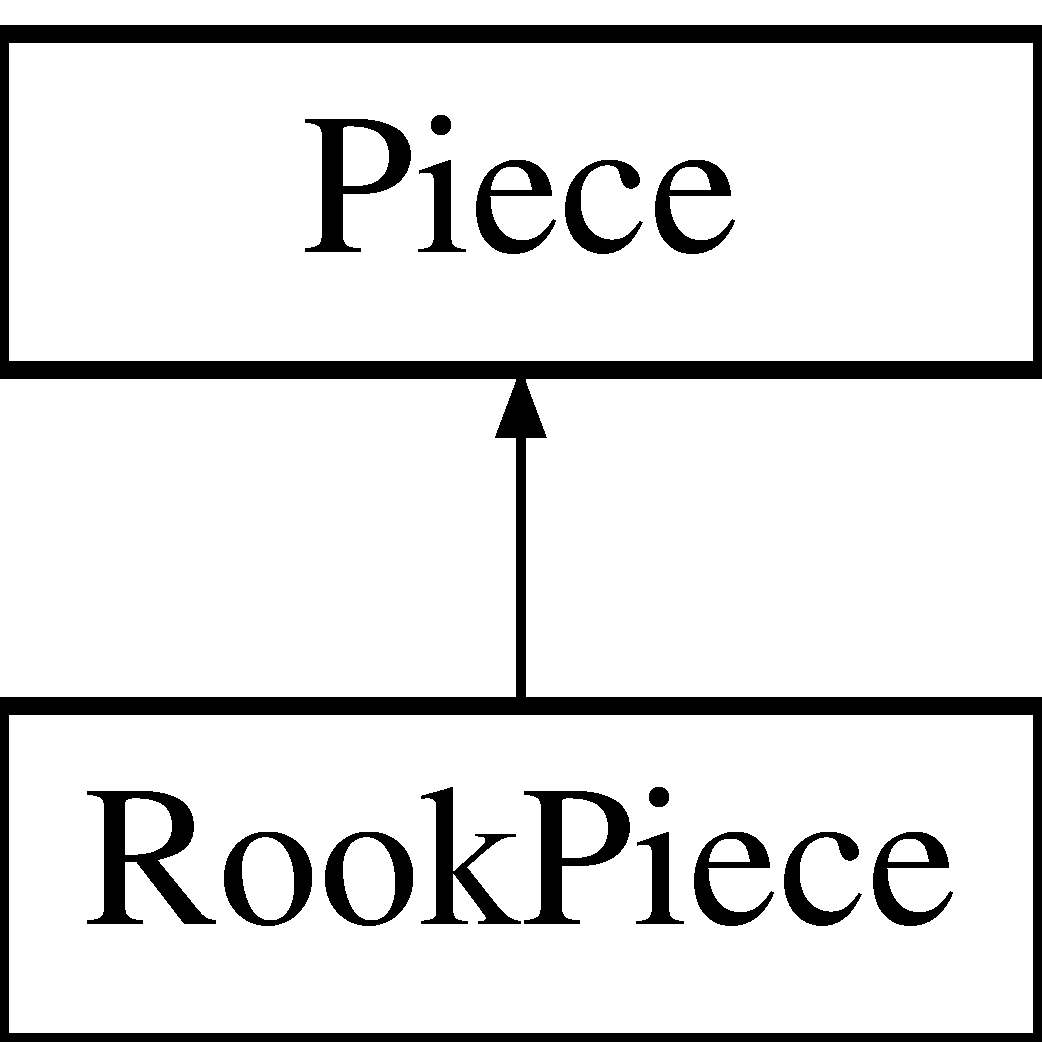
\includegraphics[height=2cm]{classRookPiece}
\end{center}
\end{figure}
\subsection*{Public Member Functions}
\begin{DoxyCompactItemize}
\item 
\hypertarget{classRookPiece_a4f3df41645f99a11dcbf3045195a9a6a}{
\hyperlink{classRookPiece_a4f3df41645f99a11dcbf3045195a9a6a}{RookPiece} (int c=0)}
\label{classRookPiece_a4f3df41645f99a11dcbf3045195a9a6a}

\begin{DoxyCompactList}\small\item\em creates a \hyperlink{classPiece}{Piece} object \item\end{DoxyCompactList}\item 
int \hyperlink{classRookPiece_a15b00afd7fe0fe1035c64b884870c6e1}{getColor} () const 
\begin{DoxyCompactList}\small\item\em gets the color of the Rook \hyperlink{classPiece}{Piece} \item\end{DoxyCompactList}\item 
void \hyperlink{classRookPiece_ad10584bf27bf3f6f109074b878ef840d}{setColor} (int colorOfPiece)
\begin{DoxyCompactList}\small\item\em sets the Color of the Rook \hyperlink{classPiece}{Piece} \item\end{DoxyCompactList}\item 
string \hyperlink{classRookPiece_a45d8858e75e550b72d27d49da0230c0a}{getType} () const 
\begin{DoxyCompactList}\small\item\em Returns Rook to user. \item\end{DoxyCompactList}\item 
int \hyperlink{classRookPiece_a451d36ccd1ccba8001acd3fff364904e}{validMove} (vector$<$ vector$<$ \hyperlink{classPiece}{Piece} $\ast$ $>$ $>$ gameBoard, int ix, int iy, int dx, int dy)
\begin{DoxyCompactList}\small\item\em validates a move based on the Rook rules. \item\end{DoxyCompactList}\end{DoxyCompactItemize}


\subsection{Detailed Description}
a class for all Rook Piece`s. 

\subsection{Member Function Documentation}
\hypertarget{classRookPiece_a15b00afd7fe0fe1035c64b884870c6e1}{
\index{RookPiece@{RookPiece}!getColor@{getColor}}
\index{getColor@{getColor}!RookPiece@{RookPiece}}
\subsubsection[{getColor}]{\setlength{\rightskip}{0pt plus 5cm}int RookPiece::getColor () const\hspace{0.3cm}{\ttfamily  \mbox{[}virtual\mbox{]}}}}
\label{classRookPiece_a15b00afd7fe0fe1035c64b884870c6e1}


gets the color of the Rook \hyperlink{classPiece}{Piece} \begin{DoxyReturn}{Returns}
int a 0 if white and 1 if black 
\end{DoxyReturn}


Implements \hyperlink{classPiece_a1376072d4815719e60253ce5688df95c}{Piece}.\hypertarget{classRookPiece_a45d8858e75e550b72d27d49da0230c0a}{
\index{RookPiece@{RookPiece}!getType@{getType}}
\index{getType@{getType}!RookPiece@{RookPiece}}
\subsubsection[{getType}]{\setlength{\rightskip}{0pt plus 5cm}string RookPiece::getType () const\hspace{0.3cm}{\ttfamily  \mbox{[}virtual\mbox{]}}}}
\label{classRookPiece_a45d8858e75e550b72d27d49da0230c0a}


Returns Rook to user. \begin{DoxyReturn}{Returns}
a string that will return Rook Type. 
\end{DoxyReturn}


Implements \hyperlink{classPiece_a5b88fcd786bb30b345b24fbc3ab24ab9}{Piece}.\hypertarget{classRookPiece_ad10584bf27bf3f6f109074b878ef840d}{
\index{RookPiece@{RookPiece}!setColor@{setColor}}
\index{setColor@{setColor}!RookPiece@{RookPiece}}
\subsubsection[{setColor}]{\setlength{\rightskip}{0pt plus 5cm}void RookPiece::setColor (int {\em colorOfPiece})\hspace{0.3cm}{\ttfamily  \mbox{[}virtual\mbox{]}}}}
\label{classRookPiece_ad10584bf27bf3f6f109074b878ef840d}


sets the Color of the Rook \hyperlink{classPiece}{Piece} 
\begin{DoxyParams}{Parameters}
\item[\mbox{$\leftarrow$} {\em colorOfPiece}]sets the Pawn Piece`s color \end{DoxyParams}


Implements \hyperlink{classPiece_a1387cb503dca308ac1e3bbe38a70a073}{Piece}.\hypertarget{classRookPiece_a451d36ccd1ccba8001acd3fff364904e}{
\index{RookPiece@{RookPiece}!validMove@{validMove}}
\index{validMove@{validMove}!RookPiece@{RookPiece}}
\subsubsection[{validMove}]{\setlength{\rightskip}{0pt plus 5cm}int RookPiece::validMove (vector$<$ vector$<$ {\bf Piece} $\ast$ $>$ $>$ {\em gameBoard}, \/  int {\em ix}, \/  int {\em iy}, \/  int {\em dx}, \/  int {\em dy})}}
\label{classRookPiece_a451d36ccd1ccba8001acd3fff364904e}


validates a move based on the Rook rules. 
\begin{DoxyParams}{Parameters}
\item[\mbox{$\leftarrow$} {\em board}]A \hyperlink{classBoard}{Board} that will contain the currect board state \item[\mbox{$\leftarrow$} {\em ix}]A int that holds the x coordinate of where the piece is moving from \item[\mbox{$\leftarrow$} {\em iy}]A int that holds the y coordinate of where the piece is moving from \item[\mbox{$\leftarrow$} {\em dx}]A int that holds the x coordinate of where the piece is moving to \item[\mbox{$\leftarrow$} {\em dy}]A int that holds the y coordinate of where the piece is moving to \end{DoxyParams}


The documentation for this class was generated from the following files:\begin{DoxyCompactItemize}
\item 
source/Piece/\hyperlink{RookPiece_8h}{RookPiece.h}\item 
source/Piece/RookPiece.cc\end{DoxyCompactItemize}

\hypertarget{classRule}{
\section{Rule Class Reference}
\label{classRule}\index{Rule@{Rule}}
}


\hyperlink{classRule}{Rule} is an Abstract base class.  


{\ttfamily \#include $<$Rule.h$>$}Inheritance diagram for Rule::\begin{figure}[H]
\begin{center}
\leavevmode
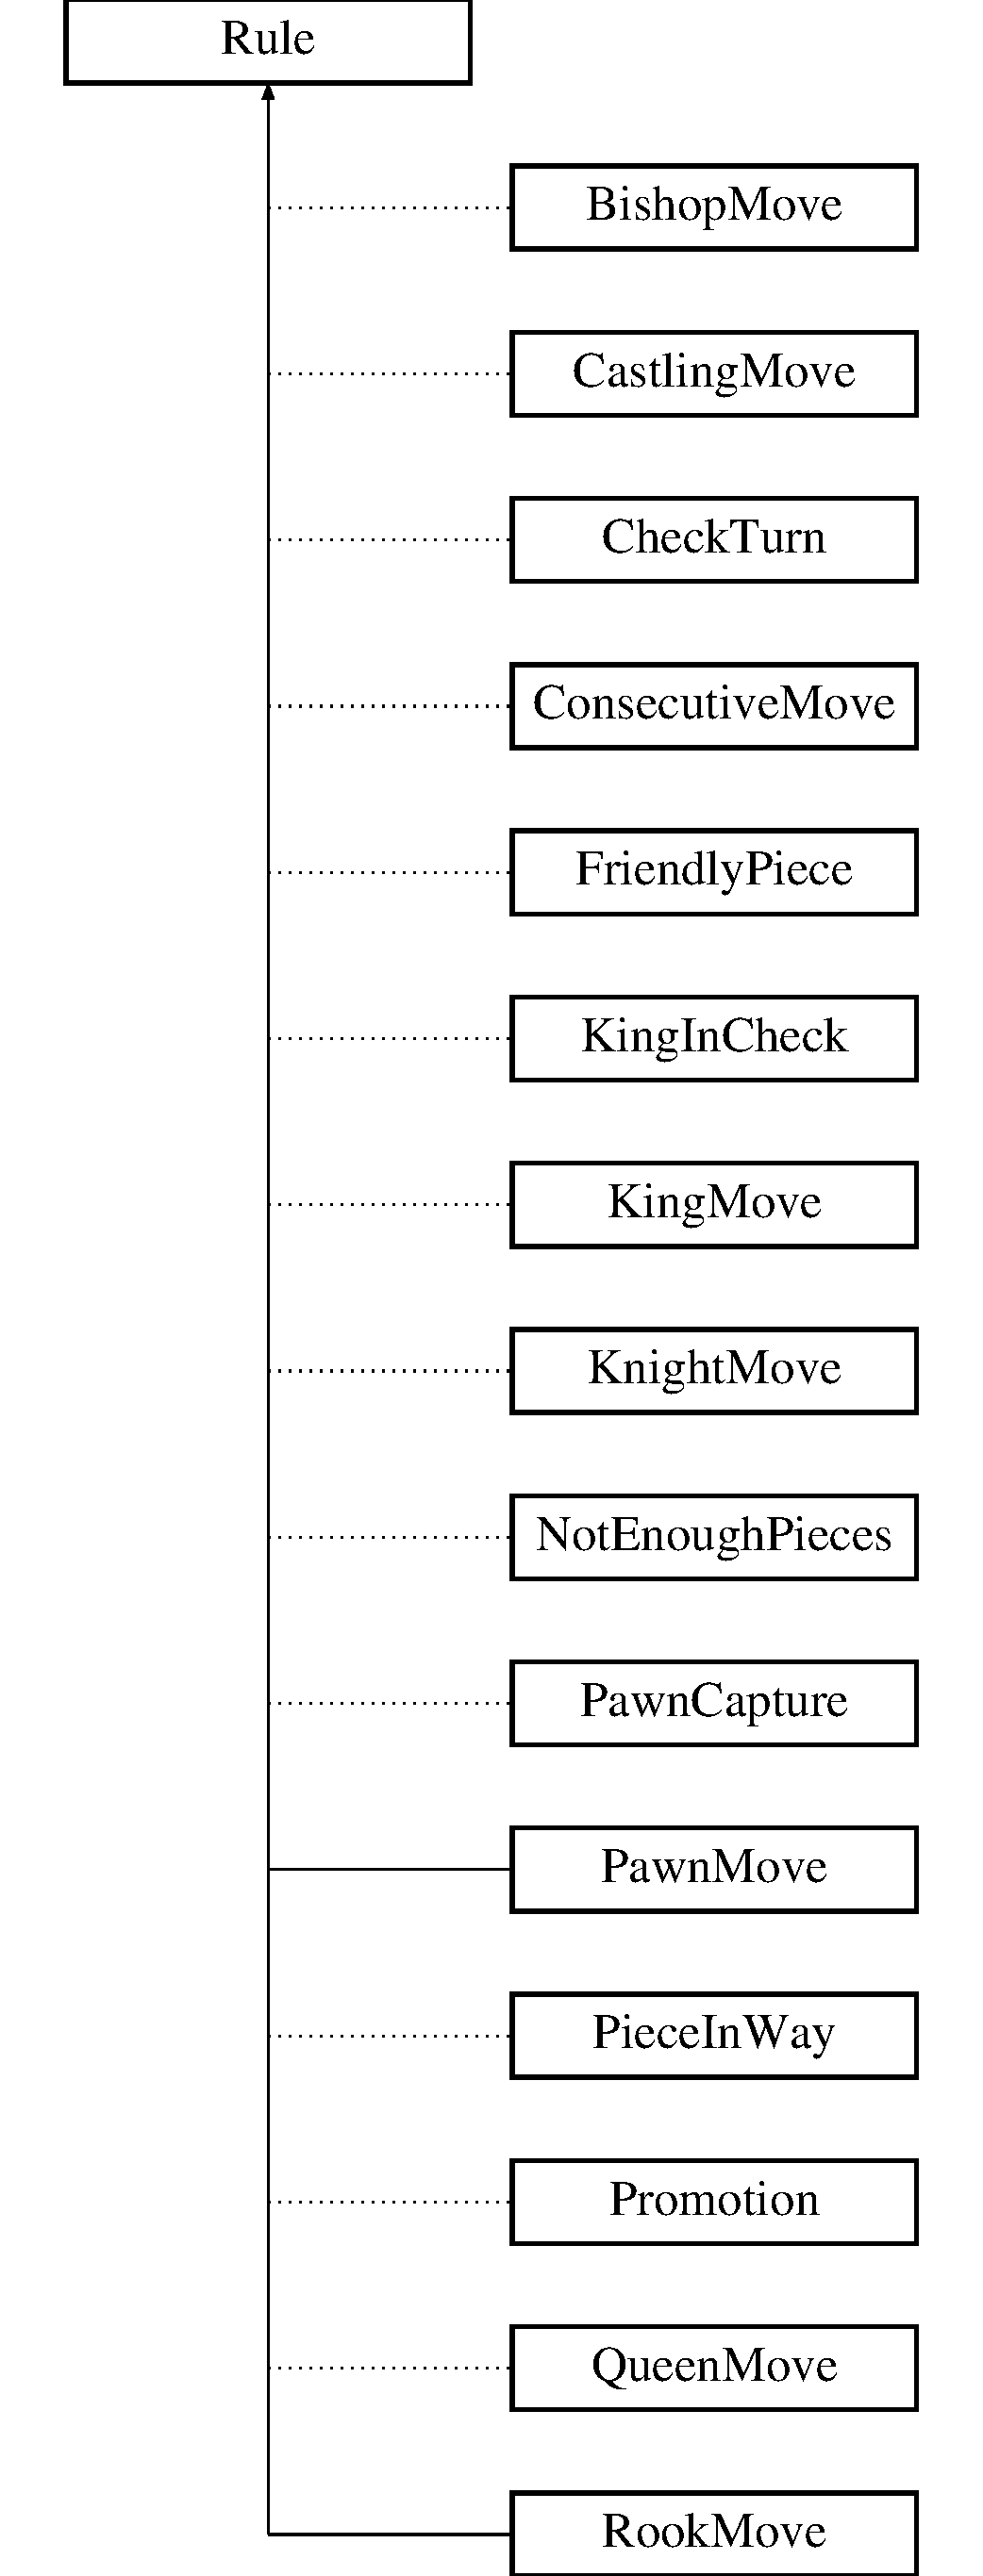
\includegraphics[height=12cm]{classRule}
\end{center}
\end{figure}


\subsection{Detailed Description}
\hyperlink{classRule}{Rule} is an Abstract base class. 

The documentation for this class was generated from the following file:\begin{DoxyCompactItemize}
\item 
source/Rules/\hyperlink{Rule_8h}{Rule.h}\end{DoxyCompactItemize}

\hypertarget{classstatus}{
\section{status Class Reference}
\label{classstatus}\index{status@{status}}
}
\subsection*{Public Member Functions}
\begin{DoxyCompactItemize}
\item 
\hypertarget{classstatus_a22e483f0410490743e4970e905e5fa19}{
\hyperlink{classstatus_a22e483f0410490743e4970e905e5fa19}{status} ()}
\label{classstatus_a22e483f0410490743e4970e905e5fa19}

\begin{DoxyCompactList}\small\item\em constructor that sets up \hyperlink{classstatus}{status}. \item\end{DoxyCompactList}\item 
\hypertarget{classstatus_aaacad1153f6cd58697d6b3871c7506ef}{
\hyperlink{classstatus_aaacad1153f6cd58697d6b3871c7506ef}{$\sim$status} ()}
\label{classstatus_aaacad1153f6cd58697d6b3871c7506ef}

\begin{DoxyCompactList}\small\item\em destructor for \hyperlink{classstatus}{status}. deletes all heap memory. \item\end{DoxyCompactList}\item 
void \hyperlink{classstatus_a350710a41204ec7fc5691e534145118e}{loadP1} (\hyperlink{classRegisteredPlayer}{RegisteredPlayer} $\ast$player)
\begin{DoxyCompactList}\small\item\em loadp1 will load a registered player onto the playerOne object \item\end{DoxyCompactList}\item 
void \hyperlink{classstatus_a09a2400aaa57b5955c3ce2987a49dcbe}{loadP2} (\hyperlink{classRegisteredPlayer}{RegisteredPlayer} $\ast$player)
\begin{DoxyCompactList}\small\item\em loadp2 will load a registered player onto the playerOne object \item\end{DoxyCompactList}\item 
\hypertarget{classstatus_a04c1417e93a7a26734da89c51ecc1596}{
void \hyperlink{classstatus_a04c1417e93a7a26734da89c51ecc1596}{Replay} ()}
\label{classstatus_a04c1417e93a7a26734da89c51ecc1596}

\begin{DoxyCompactList}\small\item\em Replay will is a switch that turns replay on or off. \item\end{DoxyCompactList}\item 
bool \hyperlink{classstatus_a7054b21075d50ee360d86b89c8b5d007}{isReplay} ()
\begin{DoxyCompactList}\small\item\em isReplay will return the \hyperlink{classstatus}{status} of replay. \item\end{DoxyCompactList}\item 
bool \hyperlink{classstatus_a20a3ca42b44610b5f37f7ca415b3ebd0}{isLoad} ()
\begin{DoxyCompactList}\small\item\em isLoad will return weather load is true or false \item\end{DoxyCompactList}\item 
void \hyperlink{classstatus_a5d04df9098e1b998605b42262e3490a8}{setReplayVector} (string fileName)
\begin{DoxyCompactList}\small\item\em setReplayVector will set the replay vector with the history vector that is being passed in. \item\end{DoxyCompactList}\item 
void \hyperlink{classstatus_af323bc43c9ac2c262599a7ce605a93d2}{setLoad} (bool set)
\begin{DoxyCompactList}\small\item\em setLoad will set weather a game is being loaded or not. \item\end{DoxyCompactList}\item 
vector$<$ string $>$ \hyperlink{classstatus_a606237d9c1b4e0ff9f2da4103aebe4de}{getReplayVector} ()
\begin{DoxyCompactList}\small\item\em setReplayVector will set the replay vector with the history vector that is being passed in. \item\end{DoxyCompactList}\item 
\hyperlink{classRegisteredPlayer}{RegisteredPlayer} $\ast$ \hyperlink{classstatus_a9f4ec14653e8e058f86e9f666e75d237}{getP1} ()
\begin{DoxyCompactList}\small\item\em getP1 will return a player pointer to the player that is stored in \hyperlink{classstatus}{status}. \item\end{DoxyCompactList}\item 
\hyperlink{classRegisteredPlayer}{RegisteredPlayer} $\ast$ \hyperlink{classstatus_a944ffb3c3b34b2def529314610337fdb}{getP2} ()
\begin{DoxyCompactList}\small\item\em getP2 will return a player pointer to the player that is stored in \hyperlink{classstatus}{status}. \item\end{DoxyCompactList}\item 
\hyperlink{classChessBoard}{ChessBoard} $\ast$ \hyperlink{classstatus_a9c563bb6d7d1b93a19a46950e0eb0c12}{getGame} ()
\begin{DoxyCompactList}\small\item\em getGame will return a pointer to the chessboard being stored in \hyperlink{classstatus}{status}. \item\end{DoxyCompactList}\item 
void \hyperlink{classstatus_a19b60728812778c97551d46403fc24bb}{setBoard} (\hyperlink{classChessBoard}{ChessBoard} $\ast$tempBoard)
\begin{DoxyCompactList}\small\item\em setBoard will set the chessboard in \hyperlink{classstatus}{status} to the one being passed in. \item\end{DoxyCompactList}\item 
string \hyperlink{classstatus_a21344f4838dff393b03f3bf6594746d7}{getP1Name} ()
\begin{DoxyCompactList}\small\item\em getP1Name will return the a string containing player ones name. \item\end{DoxyCompactList}\item 
string \hyperlink{classstatus_a4b4ad3dc4ac1444ebd6be59f6771ce0d}{getP2Name} ()
\begin{DoxyCompactList}\small\item\em getP1Name will return the a string containing player ones name. \item\end{DoxyCompactList}\item 
bool \hyperlink{classstatus_abbe7c4fa038e61cf8949432ece0defcb}{isAI} ()
\end{DoxyCompactItemize}


\subsection{Member Function Documentation}
\hypertarget{classstatus_a9c563bb6d7d1b93a19a46950e0eb0c12}{
\index{status@{status}!getGame@{getGame}}
\index{getGame@{getGame}!status@{status}}
\subsubsection[{getGame}]{\setlength{\rightskip}{0pt plus 5cm}{\bf ChessBoard} $\ast$ status::getGame ()}}
\label{classstatus_a9c563bb6d7d1b93a19a46950e0eb0c12}


getGame will return a pointer to the chessboard being stored in \hyperlink{classstatus}{status}. \begin{DoxyReturn}{Returns}
a pointer to the \hyperlink{classChessBoard}{ChessBoard} being stored in \hyperlink{classstatus}{status}. 
\end{DoxyReturn}
\hypertarget{classstatus_a9f4ec14653e8e058f86e9f666e75d237}{
\index{status@{status}!getP1@{getP1}}
\index{getP1@{getP1}!status@{status}}
\subsubsection[{getP1}]{\setlength{\rightskip}{0pt plus 5cm}{\bf RegisteredPlayer} $\ast$ status::getP1 ()}}
\label{classstatus_a9f4ec14653e8e058f86e9f666e75d237}


getP1 will return a player pointer to the player that is stored in \hyperlink{classstatus}{status}. \begin{DoxyReturn}{Returns}
a pointer to the player being stored in \hyperlink{classstatus}{status}. 
\end{DoxyReturn}
\hypertarget{classstatus_a21344f4838dff393b03f3bf6594746d7}{
\index{status@{status}!getP1Name@{getP1Name}}
\index{getP1Name@{getP1Name}!status@{status}}
\subsubsection[{getP1Name}]{\setlength{\rightskip}{0pt plus 5cm}string status::getP1Name ()}}
\label{classstatus_a21344f4838dff393b03f3bf6594746d7}


getP1Name will return the a string containing player ones name. \begin{DoxyReturn}{Returns}
a string 
\end{DoxyReturn}
\hypertarget{classstatus_a944ffb3c3b34b2def529314610337fdb}{
\index{status@{status}!getP2@{getP2}}
\index{getP2@{getP2}!status@{status}}
\subsubsection[{getP2}]{\setlength{\rightskip}{0pt plus 5cm}{\bf RegisteredPlayer} $\ast$ status::getP2 ()}}
\label{classstatus_a944ffb3c3b34b2def529314610337fdb}


getP2 will return a player pointer to the player that is stored in \hyperlink{classstatus}{status}. \begin{DoxyReturn}{Returns}
a pointer to the player being stored in \hyperlink{classstatus}{status}. 
\end{DoxyReturn}
\hypertarget{classstatus_a4b4ad3dc4ac1444ebd6be59f6771ce0d}{
\index{status@{status}!getP2Name@{getP2Name}}
\index{getP2Name@{getP2Name}!status@{status}}
\subsubsection[{getP2Name}]{\setlength{\rightskip}{0pt plus 5cm}string status::getP2Name ()}}
\label{classstatus_a4b4ad3dc4ac1444ebd6be59f6771ce0d}


getP1Name will return the a string containing player ones name. \begin{DoxyReturn}{Returns}
a string 
\end{DoxyReturn}
\hypertarget{classstatus_a606237d9c1b4e0ff9f2da4103aebe4de}{
\index{status@{status}!getReplayVector@{getReplayVector}}
\index{getReplayVector@{getReplayVector}!status@{status}}
\subsubsection[{getReplayVector}]{\setlength{\rightskip}{0pt plus 5cm}vector$<$ string $>$ status::getReplayVector ()}}
\label{classstatus_a606237d9c1b4e0ff9f2da4103aebe4de}


setReplayVector will set the replay vector with the history vector that is being passed in. 
\begin{DoxyParams}{Parameters}
\item[\mbox{$\leftarrow$} {\em filename}]is the string of the location of the vector of strings in database. \end{DoxyParams}
\hypertarget{classstatus_abbe7c4fa038e61cf8949432ece0defcb}{
\index{status@{status}!isAI@{isAI}}
\index{isAI@{isAI}!status@{status}}
\subsubsection[{isAI}]{\setlength{\rightskip}{0pt plus 5cm}bool status::isAI ()}}
\label{classstatus_abbe7c4fa038e61cf8949432ece0defcb}
this function will return a boolean on if the player 2 is a AI player or not for the multiplayer functionality \hypertarget{classstatus_a20a3ca42b44610b5f37f7ca415b3ebd0}{
\index{status@{status}!isLoad@{isLoad}}
\index{isLoad@{isLoad}!status@{status}}
\subsubsection[{isLoad}]{\setlength{\rightskip}{0pt plus 5cm}bool status::isLoad ()}}
\label{classstatus_a20a3ca42b44610b5f37f7ca415b3ebd0}


isLoad will return weather load is true or false \begin{DoxyReturn}{Returns}
return weather load is true or false. 
\end{DoxyReturn}
\hypertarget{classstatus_a7054b21075d50ee360d86b89c8b5d007}{
\index{status@{status}!isReplay@{isReplay}}
\index{isReplay@{isReplay}!status@{status}}
\subsubsection[{isReplay}]{\setlength{\rightskip}{0pt plus 5cm}bool status::isReplay ()}}
\label{classstatus_a7054b21075d50ee360d86b89c8b5d007}


isReplay will return the \hyperlink{classstatus}{status} of replay. \begin{DoxyReturn}{Returns}
returns weather \hyperlink{classstatus}{status} is true or false. 
\end{DoxyReturn}
\hypertarget{classstatus_a350710a41204ec7fc5691e534145118e}{
\index{status@{status}!loadP1@{loadP1}}
\index{loadP1@{loadP1}!status@{status}}
\subsubsection[{loadP1}]{\setlength{\rightskip}{0pt plus 5cm}void status::loadP1 ({\bf RegisteredPlayer} $\ast$ {\em player})}}
\label{classstatus_a350710a41204ec7fc5691e534145118e}


loadp1 will load a registered player onto the playerOne object 
\begin{DoxyParams}{Parameters}
\item[\mbox{$\leftarrow$} {\em player}]is a pointer to the registered player that is going to be copied. \end{DoxyParams}
\hypertarget{classstatus_a09a2400aaa57b5955c3ce2987a49dcbe}{
\index{status@{status}!loadP2@{loadP2}}
\index{loadP2@{loadP2}!status@{status}}
\subsubsection[{loadP2}]{\setlength{\rightskip}{0pt plus 5cm}void status::loadP2 ({\bf RegisteredPlayer} $\ast$ {\em player})}}
\label{classstatus_a09a2400aaa57b5955c3ce2987a49dcbe}


loadp2 will load a registered player onto the playerOne object 
\begin{DoxyParams}{Parameters}
\item[\mbox{$\leftarrow$} {\em player}]is a pointer to the registered player that is going to be copied. \end{DoxyParams}
\hypertarget{classstatus_a19b60728812778c97551d46403fc24bb}{
\index{status@{status}!setBoard@{setBoard}}
\index{setBoard@{setBoard}!status@{status}}
\subsubsection[{setBoard}]{\setlength{\rightskip}{0pt plus 5cm}void status::setBoard ({\bf ChessBoard} $\ast$ {\em tempBoard})}}
\label{classstatus_a19b60728812778c97551d46403fc24bb}


setBoard will set the chessboard in \hyperlink{classstatus}{status} to the one being passed in. 
\begin{DoxyParams}{Parameters}
\item[\mbox{$\leftarrow$} {\em tempBoard}]is the pointer to the chessboard that is being stored in \hyperlink{classstatus}{status}. \end{DoxyParams}
\hypertarget{classstatus_af323bc43c9ac2c262599a7ce605a93d2}{
\index{status@{status}!setLoad@{setLoad}}
\index{setLoad@{setLoad}!status@{status}}
\subsubsection[{setLoad}]{\setlength{\rightskip}{0pt plus 5cm}void status::setLoad (bool {\em set})}}
\label{classstatus_af323bc43c9ac2c262599a7ce605a93d2}


setLoad will set weather a game is being loaded or not. 
\begin{DoxyParams}{Parameters}
\item[\mbox{$\leftarrow$} {\em set}]is a bool value that will be coppied onto load. \end{DoxyParams}
\hypertarget{classstatus_a5d04df9098e1b998605b42262e3490a8}{
\index{status@{status}!setReplayVector@{setReplayVector}}
\index{setReplayVector@{setReplayVector}!status@{status}}
\subsubsection[{setReplayVector}]{\setlength{\rightskip}{0pt plus 5cm}void status::setReplayVector (string {\em fileName})}}
\label{classstatus_a5d04df9098e1b998605b42262e3490a8}


setReplayVector will set the replay vector with the history vector that is being passed in. 
\begin{DoxyParams}{Parameters}
\item[\mbox{$\leftarrow$} {\em filename}]is the string of the location of the vector of strings in database. \end{DoxyParams}


The documentation for this class was generated from the following files:\begin{DoxyCompactItemize}
\item 
source/status.h\item 
source/status.cc\end{DoxyCompactItemize}

\hypertarget{classTournament}{
\section{Tournament Class Reference}
\label{classTournament}\index{Tournament@{Tournament}}
}


A concrete class representing a tournament for games.  


{\ttfamily \#include $<$Tournament.h$>$}\subsection*{Public Member Functions}
\begin{DoxyCompactItemize}
\item 
\hyperlink{classTournament_af86539aa2c25a2404b7e724158371071}{Tournament} (vector$<$ string $>$ names, string tType=\char`\"{}NORMAL\char`\"{})
\begin{DoxyCompactList}\small\item\em creates a \hyperlink{classTournament}{Tournament} \item\end{DoxyCompactList}\item 
\hyperlink{classTournament_a31d8b14b4863ce1d2ece89a2f48b8b44}{Tournament} (map$<$ int, string $>$ tempRank, string tType=\char`\"{}NORMAL\char`\"{})
\item 
const vector$<$ string $>$ $\ast$ \hyperlink{classTournament_a7afa6db20cf8ae5c4b5991f2fb29e04e}{getNames} () const 
\begin{DoxyCompactList}\small\item\em gets a pointer to the vector of names in the tournament \item\end{DoxyCompactList}\item 
\hypertarget{classTournament_a9154c5a5b93249e656e7c83757085ec6}{
void \hyperlink{classTournament_a9154c5a5b93249e656e7c83757085ec6}{generateOrder} ()}
\label{classTournament_a9154c5a5b93249e656e7c83757085ec6}

\begin{DoxyCompactList}\small\item\em intialize tournament \item\end{DoxyCompactList}\item 
int \hyperlink{classTournament_ac33ed6461f737d97b0f00eb4f8ee5e10}{getCurrentMatch} () const 
\begin{DoxyCompactList}\small\item\em returns the match currently being played \item\end{DoxyCompactList}\item 
int \hyperlink{classTournament_a89b96072f94fb1393f91b026e5c42665}{getTournamentSize} () const 
\begin{DoxyCompactList}\small\item\em gets the size of the tournament \item\end{DoxyCompactList}\item 
int \hyperlink{classTournament_a3297fe5ad9a08392d8122bacb5bcf840}{getNextMatch} () const 
\begin{DoxyCompactList}\small\item\em gets the next tournament spot to be competed for \item\end{DoxyCompactList}\item 
int \hyperlink{classTournament_aedbd40e56f31c1b82e6220a0ee167ea7}{getNumPlayers} () const 
\begin{DoxyCompactList}\small\item\em gets the number of players \item\end{DoxyCompactList}\item 
void \hyperlink{classTournament_afe626f769c595b0ea1004fbc2220194d}{setMatchWinner} (string player)
\begin{DoxyCompactList}\small\item\em sets the winner of a match \item\end{DoxyCompactList}\item 
string \& \hyperlink{classTournament_a901b93c3122918e646a3c8f5625b4681}{getMatchWinner} (int spot)
\begin{DoxyCompactList}\small\item\em gets the winner of a match \item\end{DoxyCompactList}\end{DoxyCompactItemize}


\subsection{Detailed Description}
A concrete class representing a tournament for games. 

\subsection{Constructor \& Destructor Documentation}
\hypertarget{classTournament_af86539aa2c25a2404b7e724158371071}{
\index{Tournament@{Tournament}!Tournament@{Tournament}}
\index{Tournament@{Tournament}!Tournament@{Tournament}}
\subsubsection[{Tournament}]{\setlength{\rightskip}{0pt plus 5cm}Tournament::Tournament (vector$<$ string $>$ {\em names}, \/  string {\em tType} = {\ttfamily \char`\"{}NORMAL\char`\"{}})}}
\label{classTournament_af86539aa2c25a2404b7e724158371071}


creates a \hyperlink{classTournament}{Tournament} 
\begin{DoxyParams}{Parameters}
\item[\mbox{$\leftarrow$} {\em names}]A vector of strings containing the names of players \item[\mbox{$\leftarrow$} {\em tType}]tournamentType string \end{DoxyParams}
\hypertarget{classTournament_a31d8b14b4863ce1d2ece89a2f48b8b44}{
\index{Tournament@{Tournament}!Tournament@{Tournament}}
\index{Tournament@{Tournament}!Tournament@{Tournament}}
\subsubsection[{Tournament}]{\setlength{\rightskip}{0pt plus 5cm}Tournament::Tournament (map$<$ int, string $>$ {\em tempRank}, \/  string {\em tType} = {\ttfamily \char`\"{}NORMAL\char`\"{}})}}
\label{classTournament_a31d8b14b4863ce1d2ece89a2f48b8b44}
creates a \hyperlink{classTournament}{Tournament} with rank map as parameter. Useful for creating using the database loadTournament function 
\begin{DoxyParams}{Parameters}
\item[\mbox{$\leftarrow$} {\em rank}]A map containing the name and rank of players \item[\mbox{$\leftarrow$} {\em tType}]tournamentType string \end{DoxyParams}


\subsection{Member Function Documentation}
\hypertarget{classTournament_ac33ed6461f737d97b0f00eb4f8ee5e10}{
\index{Tournament@{Tournament}!getCurrentMatch@{getCurrentMatch}}
\index{getCurrentMatch@{getCurrentMatch}!Tournament@{Tournament}}
\subsubsection[{getCurrentMatch}]{\setlength{\rightskip}{0pt plus 5cm}int Tournament::getCurrentMatch () const}}
\label{classTournament_ac33ed6461f737d97b0f00eb4f8ee5e10}


returns the match currently being played \begin{DoxyReturn}{Returns}
returns the rank int of the current spot being competed for 
\end{DoxyReturn}
\hypertarget{classTournament_a901b93c3122918e646a3c8f5625b4681}{
\index{Tournament@{Tournament}!getMatchWinner@{getMatchWinner}}
\index{getMatchWinner@{getMatchWinner}!Tournament@{Tournament}}
\subsubsection[{getMatchWinner}]{\setlength{\rightskip}{0pt plus 5cm}string\& Tournament::getMatchWinner (int {\em spot})}}
\label{classTournament_a901b93c3122918e646a3c8f5625b4681}


gets the winner of a match 
\begin{DoxyParams}{Parameters}
\item[\mbox{$\leftarrow$} {\em spot}]An int representing the spot in the rank map \end{DoxyParams}
\begin{DoxyReturn}{Returns}
A string representing player that won the spot 
\end{DoxyReturn}
\hypertarget{classTournament_a7afa6db20cf8ae5c4b5991f2fb29e04e}{
\index{Tournament@{Tournament}!getNames@{getNames}}
\index{getNames@{getNames}!Tournament@{Tournament}}
\subsubsection[{getNames}]{\setlength{\rightskip}{0pt plus 5cm}const vector$<$string$>$$\ast$ Tournament::getNames () const}}
\label{classTournament_a7afa6db20cf8ae5c4b5991f2fb29e04e}


gets a pointer to the vector of names in the tournament \begin{DoxyReturn}{Returns}
returns a pointer to the vector of names in the tournament 
\end{DoxyReturn}
\hypertarget{classTournament_a3297fe5ad9a08392d8122bacb5bcf840}{
\index{Tournament@{Tournament}!getNextMatch@{getNextMatch}}
\index{getNextMatch@{getNextMatch}!Tournament@{Tournament}}
\subsubsection[{getNextMatch}]{\setlength{\rightskip}{0pt plus 5cm}int Tournament::getNextMatch () const}}
\label{classTournament_a3297fe5ad9a08392d8122bacb5bcf840}


gets the next tournament spot to be competed for \begin{DoxyReturn}{Returns}
returns the rank int of the next spot to be competed for 
\end{DoxyReturn}
\hypertarget{classTournament_aedbd40e56f31c1b82e6220a0ee167ea7}{
\index{Tournament@{Tournament}!getNumPlayers@{getNumPlayers}}
\index{getNumPlayers@{getNumPlayers}!Tournament@{Tournament}}
\subsubsection[{getNumPlayers}]{\setlength{\rightskip}{0pt plus 5cm}int Tournament::getNumPlayers () const}}
\label{classTournament_aedbd40e56f31c1b82e6220a0ee167ea7}


gets the number of players \begin{DoxyReturn}{Returns}
returns the number of players 
\end{DoxyReturn}
\hypertarget{classTournament_a89b96072f94fb1393f91b026e5c42665}{
\index{Tournament@{Tournament}!getTournamentSize@{getTournamentSize}}
\index{getTournamentSize@{getTournamentSize}!Tournament@{Tournament}}
\subsubsection[{getTournamentSize}]{\setlength{\rightskip}{0pt plus 5cm}int Tournament::getTournamentSize () const}}
\label{classTournament_a89b96072f94fb1393f91b026e5c42665}


gets the size of the tournament \begin{DoxyReturn}{Returns}
returns the an int of the size of the tournament 
\end{DoxyReturn}
\hypertarget{classTournament_afe626f769c595b0ea1004fbc2220194d}{
\index{Tournament@{Tournament}!setMatchWinner@{setMatchWinner}}
\index{setMatchWinner@{setMatchWinner}!Tournament@{Tournament}}
\subsubsection[{setMatchWinner}]{\setlength{\rightskip}{0pt plus 5cm}void Tournament::setMatchWinner (string {\em player})}}
\label{classTournament_afe626f769c595b0ea1004fbc2220194d}


sets the winner of a match 
\begin{DoxyParams}{Parameters}
\item[\mbox{$\leftarrow$} {\em spot}]An int representing the spot won in the rank map \item[\mbox{$\leftarrow$} {\em player}]A string representing player that won the spot \end{DoxyParams}


The documentation for this class was generated from the following files:\begin{DoxyCompactItemize}
\item 
source/\hyperlink{Tournament_8h}{Tournament.h}\item 
source/Tournament.cc\end{DoxyCompactItemize}

\hypertarget{classtournament__error}{
\section{tournament\_\-error Class Reference}
\label{classtournament__error}\index{tournament\_\-error@{tournament\_\-error}}
}
\subsection*{Public Member Functions}
\begin{DoxyCompactItemize}
\item 
\hyperlink{classtournament__error_ad759b11c96107b7ec10c509fec183c37}{tournament\_\-error} (const std::string \&msg)
\begin{DoxyCompactList}\small\item\em Constructor for \hyperlink{classtournament__error}{tournament\_\-error} Class. \item\end{DoxyCompactList}\end{DoxyCompactItemize}


\subsection{Constructor \& Destructor Documentation}
\hypertarget{classtournament__error_ad759b11c96107b7ec10c509fec183c37}{
\index{tournament\_\-error@{tournament\_\-error}!tournament\_\-error@{tournament\_\-error}}
\index{tournament\_\-error@{tournament\_\-error}!tournament_error@{tournament\_\-error}}
\subsubsection[{tournament\_\-error}]{\setlength{\rightskip}{0pt plus 5cm}tournament\_\-error::tournament\_\-error (const std::string \& {\em msg})\hspace{0.3cm}{\ttfamily  \mbox{[}inline\mbox{]}}}}
\label{classtournament__error_ad759b11c96107b7ec10c509fec183c37}


Constructor for \hyperlink{classtournament__error}{tournament\_\-error} Class. This is the Constructor for the \hyperlink{classtournament__error}{tournament\_\-error} class. 
\begin{DoxyParams}{Parameters}
\item[\mbox{$\leftarrow$} {\em msg}]The error message for the exception \end{DoxyParams}


The documentation for this class was generated from the following file:\begin{DoxyCompactItemize}
\item 
source/\hyperlink{Errors_8h}{Errors.h}\end{DoxyCompactItemize}

\hypertarget{classTournamentMenu}{
\section{TournamentMenu Class Reference}
\label{classTournamentMenu}\index{TournamentMenu@{TournamentMenu}}
}


\hyperlink{classTournamentMenu}{TournamentMenu} is a subclass of Generic menu.  


{\ttfamily \#include $<$TournamentMenu.h$>$}Inheritance diagram for TournamentMenu::\begin{figure}[H]
\begin{center}
\leavevmode
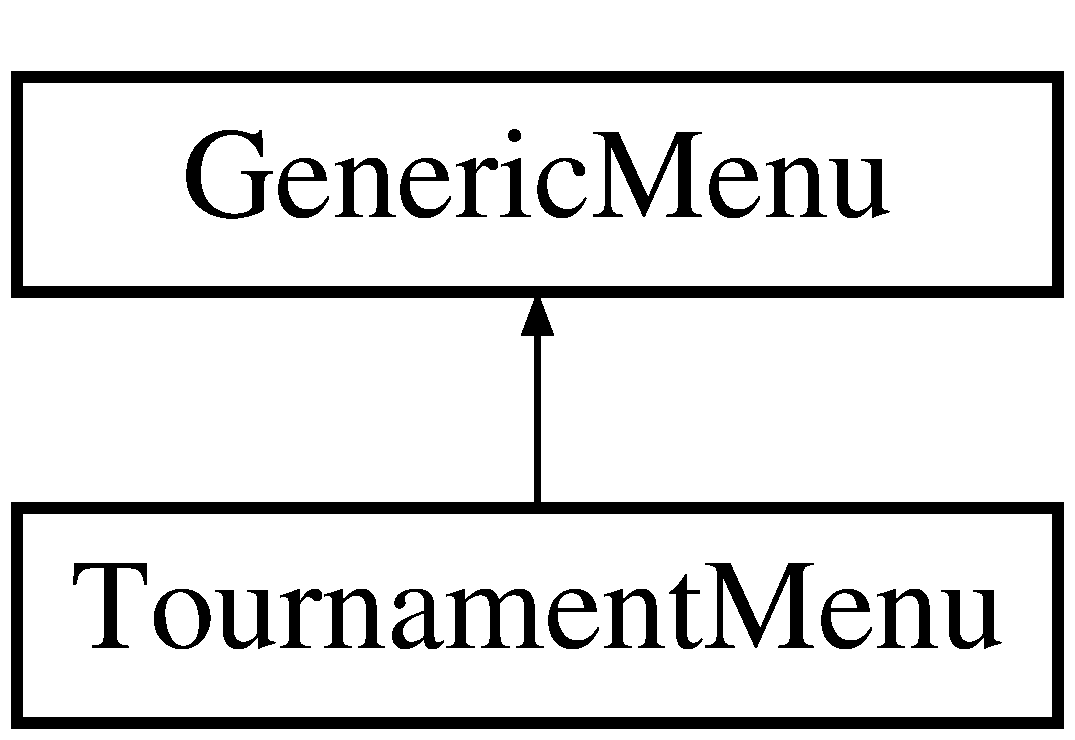
\includegraphics[height=2cm]{classTournamentMenu}
\end{center}
\end{figure}
\subsection*{Public Member Functions}
\begin{DoxyCompactItemize}
\item 
\hypertarget{classTournamentMenu_a8f635315a8f2e7ba30b1b87c867f76df}{
\hyperlink{classTournamentMenu_a8f635315a8f2e7ba30b1b87c867f76df}{TournamentMenu} ()}
\label{classTournamentMenu_a8f635315a8f2e7ba30b1b87c867f76df}

\begin{DoxyCompactList}\small\item\em \hyperlink{classTournamentMenu}{TournamentMenu} intializes all the names that will be displayed in the tournament. \item\end{DoxyCompactList}\item 
\hyperlink{classGenericMenu}{GenericMenu} $\ast$ \hyperlink{classTournamentMenu_a86ce030ba6728404ddc49aaacb45dd34}{menufunc} (string \&opt, \hyperlink{classstatus}{status} $\ast$\&info)
\begin{DoxyCompactList}\small\item\em menufunc is the general handler for implementing the functionality of this menu class \item\end{DoxyCompactList}\end{DoxyCompactItemize}


\subsection{Detailed Description}
\hyperlink{classTournamentMenu}{TournamentMenu} is a subclass of Generic menu. 

\subsection{Member Function Documentation}
\hypertarget{classTournamentMenu_a86ce030ba6728404ddc49aaacb45dd34}{
\index{TournamentMenu@{TournamentMenu}!menufunc@{menufunc}}
\index{menufunc@{menufunc}!TournamentMenu@{TournamentMenu}}
\subsubsection[{menufunc}]{\setlength{\rightskip}{0pt plus 5cm}{\bf GenericMenu} $\ast$ TournamentMenu::menufunc (string \& {\em opt}, \/  {\bf status} $\ast$\& {\em info})\hspace{0.3cm}{\ttfamily  \mbox{[}virtual\mbox{]}}}}
\label{classTournamentMenu_a86ce030ba6728404ddc49aaacb45dd34}


menufunc is the general handler for implementing the functionality of this menu class 
\begin{DoxyParams}{Parameters}
\item[\mbox{$\leftarrow$} {\em opt}]a reference for the program to decide where it must go in the main param\mbox{[}in\mbox{]} \hyperlink{classstatus}{status} is a class to enable manipulation of the current game and players between classes \end{DoxyParams}


Implements \hyperlink{classGenericMenu_a290ad7ec3331edc968190b1d7b48a397}{GenericMenu}.

The documentation for this class was generated from the following files:\begin{DoxyCompactItemize}
\item 
source/Menu/\hyperlink{TournamentMenu_8h}{TournamentMenu.h}\item 
source/Menu/\hyperlink{TournamentMenu_8cc}{TournamentMenu.cc}\end{DoxyCompactItemize}

\hypertarget{classTournamentTest}{
\section{TournamentTest Class Reference}
\label{classTournamentTest}\index{TournamentTest@{TournamentTest}}
}


{\ttfamily \#include $<$TournamentTester.h$>$}\subsection*{Public Member Functions}
\begin{DoxyCompactItemize}
\item 
\hypertarget{classTournamentTest_a3233b27bf8d8dd657239b8c841b7b029}{
void \hyperlink{classTournamentTest_a3233b27bf8d8dd657239b8c841b7b029}{setUp} ()}
\label{classTournamentTest_a3233b27bf8d8dd657239b8c841b7b029}

\begin{DoxyCompactList}\small\item\em Create variables to be used in testing. \item\end{DoxyCompactList}\item 
\hypertarget{classTournamentTest_a30942600b637d9399ac8bb90df12e279}{
void \hyperlink{classTournamentTest_a30942600b637d9399ac8bb90df12e279}{tearDown} ()}
\label{classTournamentTest_a30942600b637d9399ac8bb90df12e279}

\begin{DoxyCompactList}\small\item\em Clean up any allocated variables. \item\end{DoxyCompactList}\item 
void \hyperlink{classTournamentTest_acabeb35b05c90cb7e622e75704820422}{testGetNumPlayers} ()
\begin{DoxyCompactList}\small\item\em Testing get num players. \item\end{DoxyCompactList}\item 
\hypertarget{classTournamentTest_a9c53677756ef362f8b822a3e3dfa48bc}{
void \hyperlink{classTournamentTest_a9c53677756ef362f8b822a3e3dfa48bc}{testGetCurrentMatch} ()}
\label{classTournamentTest_a9c53677756ef362f8b822a3e3dfa48bc}

\begin{DoxyCompactList}\small\item\em Testing get current match. \item\end{DoxyCompactList}\item 
\hypertarget{classTournamentTest_ad38de1d8a2ce32a95fab531162da2475}{
void \hyperlink{classTournamentTest_ad38de1d8a2ce32a95fab531162da2475}{testGetTournamentSize} ()}
\label{classTournamentTest_ad38de1d8a2ce32a95fab531162da2475}

\begin{DoxyCompactList}\small\item\em Testing get tournament size. \item\end{DoxyCompactList}\item 
\hypertarget{classTournamentTest_a4b7aa4226a87061e56c932b3a4f6790f}{
void \hyperlink{classTournamentTest_a4b7aa4226a87061e56c932b3a4f6790f}{testGetNextMatch} ()}
\label{classTournamentTest_a4b7aa4226a87061e56c932b3a4f6790f}

\begin{DoxyCompactList}\small\item\em Testing get next match. \item\end{DoxyCompactList}\item 
\hypertarget{classTournamentTest_a0699a0def80419248e8b5feba33460d5}{
void \hyperlink{classTournamentTest_a0699a0def80419248e8b5feba33460d5}{testGetMatchWinner} ()}
\label{classTournamentTest_a0699a0def80419248e8b5feba33460d5}

\begin{DoxyCompactList}\small\item\em Testing get match winner. \item\end{DoxyCompactList}\item 
\hypertarget{classTournamentTest_a1ac8de43f0355ae6165c2bb00e45ae1b}{
void \hyperlink{classTournamentTest_a1ac8de43f0355ae6165c2bb00e45ae1b}{testSetMatchWinner} ()}
\label{classTournamentTest_a1ac8de43f0355ae6165c2bb00e45ae1b}

\begin{DoxyCompactList}\small\item\em Testing set match winner. \item\end{DoxyCompactList}\end{DoxyCompactItemize}


\subsection{Detailed Description}
Class to test \hyperlink{classTournament}{Tournament} using a fixture and a test suite 

\subsection{Member Function Documentation}
\hypertarget{classTournamentTest_acabeb35b05c90cb7e622e75704820422}{
\index{TournamentTest@{TournamentTest}!testGetNumPlayers@{testGetNumPlayers}}
\index{testGetNumPlayers@{testGetNumPlayers}!TournamentTest@{TournamentTest}}
\subsubsection[{testGetNumPlayers}]{\setlength{\rightskip}{0pt plus 5cm}void TournamentTest::testGetNumPlayers ()}}
\label{classTournamentTest_acabeb35b05c90cb7e622e75704820422}


Testing get num players. Testing get names. 

The documentation for this class was generated from the following files:\begin{DoxyCompactItemize}
\item 
tests/\hyperlink{TournamentTester_8h}{TournamentTester.h}\item 
tests/TournamentTester.cc\end{DoxyCompactItemize}

\chapter{File Documentation}
\hypertarget{Board_8h}{
\section{source/Board.h File Reference}
\label{Board_8h}\index{source/Board.h@{source/Board.h}}
}


a class that creates the \hyperlink{classBoard}{Board}.  
{\ttfamily \#include \char`\"{}Piece/Piece.h\char`\"{}}\par
{\ttfamily \#include $<$iostream$>$}\par
{\ttfamily \#include \char`\"{}Piece/BishopPiece.h\char`\"{}}\par
{\ttfamily \#include \char`\"{}Piece/PawnPiece.h\char`\"{}}\par
{\ttfamily \#include \char`\"{}Piece/RookPiece.h\char`\"{}}\par
{\ttfamily \#include \char`\"{}Piece/QueenPiece.h\char`\"{}}\par
{\ttfamily \#include \char`\"{}Piece/KingPiece.h\char`\"{}}\par
{\ttfamily \#include \char`\"{}Piece/KnightPiece.h\char`\"{}}\par
{\ttfamily \#include \char`\"{}Piece/EmptyPiece.h\char`\"{}}\par
{\ttfamily \#include \char`\"{}Definitions.h\char`\"{}}\par
{\ttfamily \#include $<$string$>$}\par
{\ttfamily \#include $<$vector$>$}\par
\subsection*{Classes}
\begin{DoxyCompactItemize}
\item 
class \hyperlink{classBoard}{Board}
\begin{DoxyCompactList}\small\item\em a concrete class for creating a board which games will be played on. \item\end{DoxyCompactList}\end{DoxyCompactItemize}


\subsection{Detailed Description}
a class that creates the \hyperlink{classBoard}{Board}. \begin{DoxyAuthor}{Author}
Marko Ilievski 
\end{DoxyAuthor}
\begin{DoxyDate}{Date}
October 27, 2014 
\end{DoxyDate}

\hypertarget{Chat_8h}{
\section{source/Chat.h File Reference}
\label{Chat_8h}\index{source/Chat.h@{source/Chat.h}}
}


a concrete class for chat functionality between players.  
{\ttfamily \#include $<$vector$>$}\par
{\ttfamily \#include $<$string$>$}\par
{\ttfamily \#include $<$utility$>$}\par
\subsection*{Classes}
\begin{DoxyCompactItemize}
\item 
class \hyperlink{classChat}{Chat}
\begin{DoxyCompactList}\small\item\em a concrete class for chat functionality between players. \item\end{DoxyCompactList}\end{DoxyCompactItemize}


\subsection{Detailed Description}
a concrete class for chat functionality between players. \begin{DoxyAuthor}{Author}
Lukas Grasse 
\end{DoxyAuthor}
\begin{DoxyDate}{Date}
October 27, 2014 
\end{DoxyDate}

\hypertarget{ChessBoard_8h}{
\section{source/ChessBoard.h File Reference}
\label{ChessBoard_8h}\index{source/ChessBoard.h@{source/ChessBoard.h}}
}


a class that creates the Chess \hyperlink{classBoard}{Board}.  
{\ttfamily \#include $<$iostream$>$}\par
{\ttfamily \#include \char`\"{}Board.h\char`\"{}}\par
{\ttfamily \#include \char`\"{}Piece/Piece.h\char`\"{}}\par
{\ttfamily \#include \char`\"{}Piece/KingPiece.h\char`\"{}}\par
{\ttfamily \#include \char`\"{}Piece/QueenPiece.h\char`\"{}}\par
{\ttfamily \#include \char`\"{}Piece/RookPiece.h\char`\"{}}\par
{\ttfamily \#include \char`\"{}Piece/BishopPiece.h\char`\"{}}\par
{\ttfamily \#include \char`\"{}Piece/KnightPiece.h\char`\"{}}\par
{\ttfamily \#include \char`\"{}Piece/PawnPiece.h\char`\"{}}\par
{\ttfamily \#include \char`\"{}Definitions.h\char`\"{}}\par
\subsection*{Classes}
\begin{DoxyCompactItemize}
\item 
class \hyperlink{classChessBoard}{ChessBoard}
\begin{DoxyCompactList}\small\item\em a concrete class for creating a chess board which games will be played on. \item\end{DoxyCompactList}\end{DoxyCompactItemize}


\subsection{Detailed Description}
a class that creates the Chess \hyperlink{classBoard}{Board}. \begin{DoxyAuthor}{Author}
Marko Ilievski 
\end{DoxyAuthor}
\begin{DoxyDate}{Date}
October 27, 2014 
\end{DoxyDate}

\hypertarget{Database_8h}{
\section{source/Database.h File Reference}
\label{Database_8h}\index{source/Database.h@{source/Database.h}}
}


a concrete class for database functionality.  
{\ttfamily \#include $<$vector$>$}\par
{\ttfamily \#include $<$string$>$}\par
{\ttfamily \#include $<$utility$>$}\par
{\ttfamily \#include $<$map$>$}\par
{\ttfamily \#include \char`\"{}Definitions.h\char`\"{}}\par
{\ttfamily \#include \char`\"{}Tournament.h\char`\"{}}\par
{\ttfamily \#include \char`\"{}Players/RegisteredPlayer.h\char`\"{}}\par
\subsection*{Classes}
\begin{DoxyCompactItemize}
\item 
class \hyperlink{classDatabase}{Database}
\begin{DoxyCompactList}\small\item\em a concrete class for database functionality for game programs. \item\end{DoxyCompactList}\end{DoxyCompactItemize}


\subsection{Detailed Description}
a concrete class for database functionality. \begin{DoxyAuthor}{Author}
Lukas Grasse 
\end{DoxyAuthor}
\begin{DoxyDate}{Date}
October 27, 2014 
\end{DoxyDate}

\hypertarget{Errors_8h}{
\section{source/Errors.h File Reference}
\label{Errors_8h}\index{source/Errors.h@{source/Errors.h}}
}
{\ttfamily \#include $<$stdexcept$>$}\par
{\ttfamily \#include $<$string$>$}\par
\subsection*{Classes}
\begin{DoxyCompactItemize}
\item 
class \hyperlink{classdatabase__load__error}{database\_\-load\_\-error}
\item 
class \hyperlink{classtournament__error}{tournament\_\-error}
\end{DoxyCompactItemize}


\subsection{Detailed Description}
file for all error classes \begin{DoxyAuthor}{Author}
Lukas Grasse 
\end{DoxyAuthor}
\begin{DoxyDate}{Date}
24-\/11-\/2014 
\end{DoxyDate}

\hypertarget{Game_8h}{
\section{source/Game.h File Reference}
\label{Game_8h}\index{source/Game.h@{source/Game.h}}
}


a class for \hyperlink{classGame}{Game}  
\subsection*{Classes}
\begin{DoxyCompactItemize}
\item 
class \hyperlink{classGame}{Game}
\end{DoxyCompactItemize}


\subsection{Detailed Description}
a class for \hyperlink{classGame}{Game} \begin{DoxyAuthor}{Author}
Zackery Shortt 
\end{DoxyAuthor}
\begin{DoxyDate}{Date}
October 27, 2014 
\end{DoxyDate}

\hypertarget{EndMenu_8cc}{
\section{source/Menu/EndMenu.cc File Reference}
\label{EndMenu_8cc}\index{source/Menu/EndMenu.cc@{source/Menu/EndMenu.cc}}
}


\hyperlink{classEndMenu}{EndMenu}.  
{\ttfamily \#include \char`\"{}EndMenu.h\char`\"{}}\par
{\ttfamily \#include $<$string$>$}\par
{\ttfamily \#include $<$iomanip$>$}\par
{\ttfamily \#include $<$iostream$>$}\par
{\ttfamily \#include \char`\"{}LeaderBoard.h\char`\"{}}\par
{\ttfamily \#include \char`\"{}MainMenu.h\char`\"{}}\par


\subsection{Detailed Description}
\hyperlink{classEndMenu}{EndMenu}. \begin{DoxyAuthor}{Author}
Michael Wilson, Brandon Robertson. 
\end{DoxyAuthor}
\begin{DoxyDate}{Date}
October 26,2014 
\end{DoxyDate}

\hypertarget{EndMenu_8h}{
\section{source/Menu/EndMenu.h File Reference}
\label{EndMenu_8h}\index{source/Menu/EndMenu.h@{source/Menu/EndMenu.h}}
}


a base class for all menus.  
{\ttfamily \#include \char`\"{}GenericMenu.h\char`\"{}}\par
{\ttfamily \#include $<$string$>$}\par
{\ttfamily \#include \char`\"{}../status.h\char`\"{}}\par
\subsection*{Classes}
\begin{DoxyCompactItemize}
\item 
class \hyperlink{classEndMenu}{EndMenu}
\begin{DoxyCompactList}\small\item\em \hyperlink{classEndMenu}{EndMenu} is a subclass of \hyperlink{classGenericMenu}{GenericMenu}. \item\end{DoxyCompactList}\end{DoxyCompactItemize}


\subsection{Detailed Description}
a base class for all menus. \begin{DoxyAuthor}{Author}
Michael Wilson, Brandon Robertson. 
\end{DoxyAuthor}
\begin{DoxyDate}{Date}
October 26,2014 
\end{DoxyDate}

\hypertarget{GenericMenu_8h}{
\section{source/Menu/GenericMenu.h File Reference}
\label{GenericMenu_8h}\index{source/Menu/GenericMenu.h@{source/Menu/GenericMenu.h}}
}


a base class for all menus.  
{\ttfamily \#include $<$string$>$}\par
{\ttfamily \#include \char`\"{}../status.h\char`\"{}}\par
\subsection*{Classes}
\begin{DoxyCompactItemize}
\item 
class \hyperlink{classGenericMenu}{GenericMenu}
\begin{DoxyCompactList}\small\item\em \hyperlink{classGenericMenu}{GenericMenu} super class of all menus. \item\end{DoxyCompactList}\end{DoxyCompactItemize}


\subsection{Detailed Description}
a base class for all menus. \begin{DoxyAuthor}{Author}
Michael Wilson, Brandon Robertson. 
\end{DoxyAuthor}
\begin{DoxyDate}{Date}
October 26,2014 
\end{DoxyDate}

\hypertarget{LeaderBoard_8cc}{
\section{source/Menu/LeaderBoard.cc File Reference}
\label{LeaderBoard_8cc}\index{source/Menu/LeaderBoard.cc@{source/Menu/LeaderBoard.cc}}
}


\hyperlink{classLeaderBoard}{LeaderBoard} class.  
{\ttfamily \#include \char`\"{}LeaderBoard.h\char`\"{}}\par
{\ttfamily \#include \char`\"{}MainMenu.h\char`\"{}}\par
{\ttfamily \#include \char`\"{}../Database.h\char`\"{}}\par


\subsection{Detailed Description}
\hyperlink{classLeaderBoard}{LeaderBoard} class. \begin{DoxyAuthor}{Author}
Michael Wilson, Brandon Robertson. 
\end{DoxyAuthor}
\begin{DoxyDate}{Date}
October 26,2014 
\end{DoxyDate}

\hypertarget{LeaderBoard_8h}{
\section{source/Menu/LeaderBoard.h File Reference}
\label{LeaderBoard_8h}\index{source/Menu/LeaderBoard.h@{source/Menu/LeaderBoard.h}}
}


a base class for all menus.  
{\ttfamily \#include \char`\"{}GenericMenu.h\char`\"{}}\par
{\ttfamily \#include $<$string$>$}\par
{\ttfamily \#include $<$iomanip$>$}\par
{\ttfamily \#include $<$iostream$>$}\par
{\ttfamily \#include \char`\"{}../Players/Player.h\char`\"{}}\par
{\ttfamily \#include \char`\"{}../Players/RegisteredPlayer.h\char`\"{}}\par
{\ttfamily \#include \char`\"{}../Database.h\char`\"{}}\par
{\ttfamily \#include \char`\"{}../Definitions.h\char`\"{}}\par
{\ttfamily \#include $<$vector$>$}\par
{\ttfamily \#include \char`\"{}MainMenu.h\char`\"{}}\par
{\ttfamily \#include \char`\"{}../status.h\char`\"{}}\par
\subsection*{Classes}
\begin{DoxyCompactItemize}
\item 
class \hyperlink{classLeaderBoard}{LeaderBoard}
\end{DoxyCompactItemize}


\subsection{Detailed Description}
a base class for all menus. \begin{DoxyAuthor}{Author}
Michael Wilson, Brandon Robertson. 
\end{DoxyAuthor}
\begin{DoxyDate}{Date}
October 26,2014 
\end{DoxyDate}

\hypertarget{LoginMenu_8cc}{
\section{source/Menu/LoginMenu.cc File Reference}
\label{LoginMenu_8cc}\index{source/Menu/LoginMenu.cc@{source/Menu/LoginMenu.cc}}
}


loginMenu class  
{\ttfamily \#include \char`\"{}LoginMenu.h\char`\"{}}\par
{\ttfamily \#include $<$string$>$}\par
{\ttfamily \#include $<$iomanip$>$}\par
{\ttfamily \#include $<$iostream$>$}\par
{\ttfamily \#include \char`\"{}MainMenu.h\char`\"{}}\par
{\ttfamily \#include \char`\"{}../Players/Player.h\char`\"{}}\par
{\ttfamily \#include \char`\"{}../Players/RegisteredPlayer.h\char`\"{}}\par
{\ttfamily \#include \char`\"{}../Database.h\char`\"{}}\par
{\ttfamily \#include \char`\"{}../Definitions.h\char`\"{}}\par


\subsection{Detailed Description}
loginMenu class \begin{DoxyAuthor}{Author}
Michael Wilson, Brandon Robertson. 
\end{DoxyAuthor}
\begin{DoxyDate}{Date}
October 26,2014 
\end{DoxyDate}

\hypertarget{LoginMenu_8h}{
\section{source/Menu/LoginMenu.h File Reference}
\label{LoginMenu_8h}\index{source/Menu/LoginMenu.h@{source/Menu/LoginMenu.h}}
}


loginMenu header  
{\ttfamily \#include \char`\"{}GenericMenu.h\char`\"{}}\par
{\ttfamily \#include $<$iostream$>$}\par
{\ttfamily \#include $<$string$>$}\par
{\ttfamily \#include \char`\"{}../Players/Player.h\char`\"{}}\par
{\ttfamily \#include \char`\"{}../status.h\char`\"{}}\par
{\ttfamily \#include \char`\"{}../Players/RegisteredPlayer.h\char`\"{}}\par
\subsection*{Classes}
\begin{DoxyCompactItemize}
\item 
class \hyperlink{classLoginMenu}{LoginMenu}
\end{DoxyCompactItemize}


\subsection{Detailed Description}
loginMenu header \begin{DoxyAuthor}{Author}
Michael Wilson, Brandon Robertson. 
\end{DoxyAuthor}
\begin{DoxyDate}{Date}
October 26,2014 
\end{DoxyDate}

\hypertarget{MainMenu_8cc}{
\section{source/Menu/MainMenu.cc File Reference}
\label{MainMenu_8cc}\index{source/Menu/MainMenu.cc@{source/Menu/MainMenu.cc}}
}


mainMenu class  
{\ttfamily \#include \char`\"{}MainMenu.h\char`\"{}}\par
{\ttfamily \#include \char`\"{}GenericMenu.h\char`\"{}}\par
{\ttfamily \#include $<$iostream$>$}\par
{\ttfamily \#include $<$iomanip$>$}\par
{\ttfamily \#include \char`\"{}LeaderBoard.h\char`\"{}}\par
{\ttfamily \#include \char`\"{}TournamentMenu.h\char`\"{}}\par
{\ttfamily \#include \char`\"{}LoginMenu.h\char`\"{}}\par
{\ttfamily \#include \char`\"{}../chessGameGUI.h\char`\"{}}\par
{\ttfamily \#include \char`\"{}../status.h\char`\"{}}\par
{\ttfamily \#include \char`\"{}../Players/Player.h\char`\"{}}\par
{\ttfamily \#include \char`\"{}../Database.h\char`\"{}}\par
{\ttfamily \#include \char`\"{}../Errors.h\char`\"{}}\par


\subsection{Detailed Description}
mainMenu class \begin{DoxyAuthor}{Author}
Michael Wilson, Brandon Robertson. 
\end{DoxyAuthor}
\begin{DoxyDate}{Date}
October 26,2014 
\end{DoxyDate}

\hypertarget{MainMenu_8h}{
\section{source/Menu/MainMenu.h File Reference}
\label{MainMenu_8h}\index{source/Menu/MainMenu.h@{source/Menu/MainMenu.h}}
}


mainMenu header  
{\ttfamily \#include \char`\"{}GenericMenu.h\char`\"{}}\par
{\ttfamily \#include \char`\"{}../status.h\char`\"{}}\par
\subsection*{Classes}
\begin{DoxyCompactItemize}
\item 
class \hyperlink{classMainMenu}{MainMenu}
\end{DoxyCompactItemize}


\subsection{Detailed Description}
mainMenu header \begin{DoxyAuthor}{Author}
Michael Wilson, Brandon Robertson. 
\end{DoxyAuthor}
\begin{DoxyDate}{Date}
October 26,2014 
\end{DoxyDate}

\hypertarget{PauseMenu_8cc}{
\section{source/Menu/PauseMenu.cc File Reference}
\label{PauseMenu_8cc}\index{source/Menu/PauseMenu.cc@{source/Menu/PauseMenu.cc}}
}


\hyperlink{classPauseMenu}{PauseMenu} class.  
{\ttfamily \#include \char`\"{}PauseMenu.h\char`\"{}}\par
{\ttfamily \#include $<$string$>$}\par
{\ttfamily \#include $<$iomanip$>$}\par
{\ttfamily \#include $<$iostream$>$}\par
{\ttfamily \#include \char`\"{}LeaderBoard.h\char`\"{}}\par
{\ttfamily \#include \char`\"{}MainMenu.h\char`\"{}}\par
{\ttfamily \#include \char`\"{}../Database.h\char`\"{}}\par
{\ttfamily \#include \char`\"{}../ChessBoard.h\char`\"{}}\par
{\ttfamily \#include \char`\"{}../chessGameGUI.h\char`\"{}}\par
{\ttfamily \#include $<$unistd.h$>$}\par


\subsection{Detailed Description}
\hyperlink{classPauseMenu}{PauseMenu} class. \begin{DoxyAuthor}{Author}
Michael Wilson, Brandon Robertson. 
\end{DoxyAuthor}
\begin{DoxyDate}{Date}
October 26,2014 
\end{DoxyDate}

\hypertarget{PauseMenu_8h}{
\section{source/Menu/PauseMenu.h File Reference}
\label{PauseMenu_8h}\index{source/Menu/PauseMenu.h@{source/Menu/PauseMenu.h}}
}


a base class for all menus.  
{\ttfamily \#include \char`\"{}GenericMenu.h\char`\"{}}\par
{\ttfamily \#include \char`\"{}../status.h\char`\"{}}\par
\subsection*{Classes}
\begin{DoxyCompactItemize}
\item 
class \hyperlink{classPauseMenu}{PauseMenu}
\begin{DoxyCompactList}\small\item\em \hyperlink{classPauseMenu}{PauseMenu} is a subclass of Generic Menu. \item\end{DoxyCompactList}\end{DoxyCompactItemize}


\subsection{Detailed Description}
a base class for all menus. \begin{DoxyAuthor}{Author}
Michael Wilson, Brandon Robertson. 
\end{DoxyAuthor}
\begin{DoxyDate}{Date}
October 26,2014 
\end{DoxyDate}

\hypertarget{TournamentMenu_8cc}{
\section{source/Menu/TournamentMenu.cc File Reference}
\label{TournamentMenu_8cc}\index{source/Menu/TournamentMenu.cc@{source/Menu/TournamentMenu.cc}}
}


tournament class.  
{\ttfamily \#include $<$iostream$>$}\par
{\ttfamily \#include $<$string$>$}\par
{\ttfamily \#include $<$iomanip$>$}\par
{\ttfamily \#include \char`\"{}TournamentMenu.h\char`\"{}}\par
{\ttfamily \#include \char`\"{}GenericMenu.h\char`\"{}}\par
{\ttfamily \#include \char`\"{}MainMenu.h\char`\"{}}\par
{\ttfamily \#include $<$cassert$>$}\par
{\ttfamily \#include \char`\"{}../Tournament.h\char`\"{}}\par
{\ttfamily \#include \char`\"{}../Database.h\char`\"{}}\par
{\ttfamily \#include \char`\"{}../Players/Player.h\char`\"{}}\par
{\ttfamily \#include $<$map$>$}\par


\subsection{Detailed Description}
tournament class. \begin{DoxyAuthor}{Author}
Michael Wilson, Brandon Robertson. 
\end{DoxyAuthor}
\begin{DoxyDate}{Date}
October 26,2014 
\end{DoxyDate}

\hypertarget{TournamentMenu_8h}{
\section{source/Menu/TournamentMenu.h File Reference}
\label{TournamentMenu_8h}\index{source/Menu/TournamentMenu.h@{source/Menu/TournamentMenu.h}}
}


a class for tournament menu.  
{\ttfamily \#include \char`\"{}GenericMenu.h\char`\"{}}\par
{\ttfamily \#include $<$string$>$}\par
{\ttfamily \#include \char`\"{}../status.h\char`\"{}}\par
{\ttfamily \#include \char`\"{}../Tournament.h\char`\"{}}\par
\subsection*{Classes}
\begin{DoxyCompactItemize}
\item 
class \hyperlink{classTournamentMenu}{TournamentMenu}
\begin{DoxyCompactList}\small\item\em \hyperlink{classTournamentMenu}{TournamentMenu} is a subclass of Generic menu. \item\end{DoxyCompactList}\end{DoxyCompactItemize}


\subsection{Detailed Description}
a class for tournament menu. Michael Wilson, Brandon Robertson. \begin{DoxyDate}{Date}
October 26, 2014 
\end{DoxyDate}

\hypertarget{BishopPiece_8h}{
\section{source/Piece/BishopPiece.h File Reference}
\label{BishopPiece_8h}\index{source/Piece/BishopPiece.h@{source/Piece/BishopPiece.h}}
}


class for the Bishop \hyperlink{classPiece}{Piece}  
{\ttfamily \#include \char`\"{}Piece.h\char`\"{}}\par
{\ttfamily \#include $<$string$>$}\par
{\ttfamily \#include $<$vector$>$}\par
{\ttfamily \#include \char`\"{}../Rules/BishopMove.h\char`\"{}}\par
\subsection*{Classes}
\begin{DoxyCompactItemize}
\item 
class \hyperlink{classBishopPiece}{BishopPiece}
\begin{DoxyCompactList}\small\item\em a class for all Bishop Piece`s. \item\end{DoxyCompactList}\end{DoxyCompactItemize}


\subsection{Detailed Description}
class for the Bishop \hyperlink{classPiece}{Piece} \begin{DoxyAuthor}{Author}
Marko Ilievski 
\end{DoxyAuthor}
\begin{DoxyDate}{Date}
October 27, 2014 
\end{DoxyDate}

\hypertarget{EmptyPiece_8h}{
\section{source/Piece/EmptyPiece.h File Reference}
\label{EmptyPiece_8h}\index{source/Piece/EmptyPiece.h@{source/Piece/EmptyPiece.h}}
}


class for the Pawn \hyperlink{classPiece}{Piece}  
{\ttfamily \#include \char`\"{}Piece.h\char`\"{}}\par
{\ttfamily \#include $<$string$>$}\par
{\ttfamily \#include $<$vector$>$}\par
\subsection*{Classes}
\begin{DoxyCompactItemize}
\item 
class \hyperlink{classEmptyPiece}{EmptyPiece}
\begin{DoxyCompactList}\small\item\em a class for all Pawn Piece`s. \item\end{DoxyCompactList}\end{DoxyCompactItemize}


\subsection{Detailed Description}
class for the Pawn \hyperlink{classPiece}{Piece} \begin{DoxyAuthor}{Author}
Marko Ilievski 
\end{DoxyAuthor}
\begin{DoxyDate}{Date}
October 27, 2014 
\end{DoxyDate}

\hypertarget{KingPiece_8h}{
\section{source/Piece/KingPiece.h File Reference}
\label{KingPiece_8h}\index{source/Piece/KingPiece.h@{source/Piece/KingPiece.h}}
}


class for the King \hyperlink{classPiece}{Piece}  
{\ttfamily \#include \char`\"{}Piece.h\char`\"{}}\par
{\ttfamily \#include $<$string$>$}\par
{\ttfamily \#include $<$vector$>$}\par
{\ttfamily \#include \char`\"{}../Rules/KingMove.h\char`\"{}}\par
\subsection*{Classes}
\begin{DoxyCompactItemize}
\item 
class \hyperlink{classKingPiece}{KingPiece}
\begin{DoxyCompactList}\small\item\em a class for all King Piece`s. \item\end{DoxyCompactList}\end{DoxyCompactItemize}


\subsection{Detailed Description}
class for the King \hyperlink{classPiece}{Piece} \begin{DoxyAuthor}{Author}
Marko Ilievski 
\end{DoxyAuthor}
\begin{DoxyDate}{Date}
October 27, 2014 
\end{DoxyDate}

\hypertarget{KnightPiece_8h}{
\section{source/Piece/KnightPiece.h File Reference}
\label{KnightPiece_8h}\index{source/Piece/KnightPiece.h@{source/Piece/KnightPiece.h}}
}


class for the Knight \hyperlink{classPiece}{Piece}  
{\ttfamily \#include \char`\"{}Piece.h\char`\"{}}\par
{\ttfamily \#include $<$string$>$}\par
{\ttfamily \#include $<$vector$>$}\par
{\ttfamily \#include \char`\"{}../Rules/KnightMove.h\char`\"{}}\par
\subsection*{Classes}
\begin{DoxyCompactItemize}
\item 
class \hyperlink{classKnightPiece}{KnightPiece}
\begin{DoxyCompactList}\small\item\em a class for all Knight Piece`s. \item\end{DoxyCompactList}\end{DoxyCompactItemize}


\subsection{Detailed Description}
class for the Knight \hyperlink{classPiece}{Piece} \begin{DoxyAuthor}{Author}
Marko Ilievski 
\end{DoxyAuthor}
\begin{DoxyDate}{Date}
October 27, 2014 
\end{DoxyDate}

\hypertarget{PawnPiece_8h}{
\section{source/Piece/PawnPiece.h File Reference}
\label{PawnPiece_8h}\index{source/Piece/PawnPiece.h@{source/Piece/PawnPiece.h}}
}


class for the Pawn \hyperlink{classPiece}{Piece}  
{\ttfamily \#include \char`\"{}Piece.h\char`\"{}}\par
{\ttfamily \#include $<$string$>$}\par
{\ttfamily \#include $<$vector$>$}\par
{\ttfamily \#include \char`\"{}../Rules/PawnMove.h\char`\"{}}\par
\subsection*{Classes}
\begin{DoxyCompactItemize}
\item 
class \hyperlink{classPawnPiece}{PawnPiece}
\begin{DoxyCompactList}\small\item\em a class for all Pawn Piece`s. \item\end{DoxyCompactList}\end{DoxyCompactItemize}


\subsection{Detailed Description}
class for the Pawn \hyperlink{classPiece}{Piece} \begin{DoxyAuthor}{Author}
Marko Ilievski 
\end{DoxyAuthor}
\begin{DoxyDate}{Date}
October 27, 2014 
\end{DoxyDate}

\hypertarget{Piece_8h}{
\section{source/Piece/Piece.h File Reference}
\label{Piece_8h}\index{source/Piece/Piece.h@{source/Piece/Piece.h}}
}


a base class for Piece`s  
{\ttfamily \#include $<$iostream$>$}\par
{\ttfamily \#include $<$string$>$}\par
{\ttfamily \#include $<$vector$>$}\par
\subsection*{Classes}
\begin{DoxyCompactItemize}
\item 
class \hyperlink{classPiece}{Piece}
\begin{DoxyCompactList}\small\item\em a a base class that will be inherited by all other Piece`s. \item\end{DoxyCompactList}\end{DoxyCompactItemize}


\subsection{Detailed Description}
a base class for Piece`s \begin{DoxyAuthor}{Author}
Marko Ilievski 
\end{DoxyAuthor}
\begin{DoxyDate}{Date}
October 27, 2014 
\end{DoxyDate}

\hypertarget{QueenPiece_8h}{
\section{source/Piece/QueenPiece.h File Reference}
\label{QueenPiece_8h}\index{source/Piece/QueenPiece.h@{source/Piece/QueenPiece.h}}
}


class for the Queen \hyperlink{classPiece}{Piece}  
{\ttfamily \#include \char`\"{}Piece.h\char`\"{}}\par
{\ttfamily \#include $<$string$>$}\par
{\ttfamily \#include $<$vector$>$}\par
{\ttfamily \#include \char`\"{}../Rules/QueenMove.h\char`\"{}}\par
\subsection*{Classes}
\begin{DoxyCompactItemize}
\item 
class \hyperlink{classQueenPiece}{QueenPiece}
\begin{DoxyCompactList}\small\item\em a class for all Queen Piece`s. \item\end{DoxyCompactList}\end{DoxyCompactItemize}


\subsection{Detailed Description}
class for the Queen \hyperlink{classPiece}{Piece} \begin{DoxyAuthor}{Author}
Marko Ilievski 
\end{DoxyAuthor}
\begin{DoxyDate}{Date}
October 27, 2014 
\end{DoxyDate}

\hypertarget{RookPiece_8h}{
\section{source/Piece/RookPiece.h File Reference}
\label{RookPiece_8h}\index{source/Piece/RookPiece.h@{source/Piece/RookPiece.h}}
}


class for the Rook \hyperlink{classPiece}{Piece}  
{\ttfamily \#include $<$vector$>$}\par
{\ttfamily \#include \char`\"{}Piece.h\char`\"{}}\par
{\ttfamily \#include $<$string$>$}\par
{\ttfamily \#include \char`\"{}../Rules/RookMove.h\char`\"{}}\par
\subsection*{Classes}
\begin{DoxyCompactItemize}
\item 
class \hyperlink{classRookPiece}{RookPiece}
\begin{DoxyCompactList}\small\item\em a class for all Rook Piece`s. \item\end{DoxyCompactList}\end{DoxyCompactItemize}


\subsection{Detailed Description}
class for the Rook \hyperlink{classPiece}{Piece} \begin{DoxyAuthor}{Author}
Marko Ilievski 
\end{DoxyAuthor}
\begin{DoxyDate}{Date}
October 27, 2014 
\end{DoxyDate}

\hypertarget{BishopMove_8h}{
\section{source/Rules/BishopMove.h File Reference}
\label{BishopMove_8h}\index{source/Rules/BishopMove.h@{source/Rules/BishopMove.h}}
}


a subclass of the rule class.  
{\ttfamily \#include $<$vector$>$}\par
{\ttfamily \#include \char`\"{}Rule.h\char`\"{}}\par
{\ttfamily \#include \char`\"{}PieceInWay.h\char`\"{}}\par
\subsection*{Classes}
\begin{DoxyCompactItemize}
\item 
class \hyperlink{classBishopMove}{BishopMove}
\end{DoxyCompactItemize}


\subsection{Detailed Description}
a subclass of the rule class. \begin{DoxyAuthor}{Author}
Michael Wilson. 
\end{DoxyAuthor}
\begin{DoxyDate}{Date}
October 27,2014 
\end{DoxyDate}

\hypertarget{CastlingMove_8h}{
\section{source/Rules/CastlingMove.h File Reference}
\label{CastlingMove_8h}\index{source/Rules/CastlingMove.h@{source/Rules/CastlingMove.h}}
}


a subclass of the rule class.  
{\ttfamily \#include $<$vector$>$}\par
{\ttfamily \#include \char`\"{}Rule.h\char`\"{}}\par
{\ttfamily \#include \char`\"{}PieceInWay.h\char`\"{}}\par
\subsection*{Classes}
\begin{DoxyCompactItemize}
\item 
class \hyperlink{classCastlingMove}{CastlingMove}
\end{DoxyCompactItemize}


\subsection{Detailed Description}
a subclass of the rule class. \begin{DoxyAuthor}{Author}
Michael Wilson. 
\end{DoxyAuthor}
\begin{DoxyDate}{Date}
October 27,2014 
\end{DoxyDate}

\hypertarget{CheckTurn_8h}{
\section{source/Rules/CheckTurn.h File Reference}
\label{CheckTurn_8h}\index{source/Rules/CheckTurn.h@{source/Rules/CheckTurn.h}}
}


a subclass of the rule class.  
{\ttfamily \#include $<$vector$>$}\par
{\ttfamily \#include \char`\"{}Rule.h\char`\"{}}\par
{\ttfamily \#include \char`\"{}KingInCheck.h\char`\"{}}\par
{\ttfamily \#include \char`\"{}../Definitions.h\char`\"{}}\par
\subsection*{Classes}
\begin{DoxyCompactItemize}
\item 
class \hyperlink{classCheckTurn}{CheckTurn}
\end{DoxyCompactItemize}


\subsection{Detailed Description}
a subclass of the rule class. \begin{DoxyAuthor}{Author}
Michael Wilson. 
\end{DoxyAuthor}
\begin{DoxyDate}{Date}
October 27,2014 
\end{DoxyDate}

\hypertarget{ConsecutiveMove_8h}{
\section{source/Rules/ConsecutiveMove.h File Reference}
\label{ConsecutiveMove_8h}\index{source/Rules/ConsecutiveMove.h@{source/Rules/ConsecutiveMove.h}}
}


a sublass of the rule class.  
{\ttfamily \#include $<$vector$>$}\par
{\ttfamily \#include \char`\"{}Rule.h\char`\"{}}\par
{\ttfamily \#include \char`\"{}NotEnoughPieces.h\char`\"{}}\par
{\ttfamily \#include \char`\"{}../Definitions.h\char`\"{}}\par
\subsection*{Classes}
\begin{DoxyCompactItemize}
\item 
class \hyperlink{classConsecutiveMove}{ConsecutiveMove}
\end{DoxyCompactItemize}


\subsection{Detailed Description}
a sublass of the rule class. \begin{DoxyAuthor}{Author}
Michael Wilson. 
\end{DoxyAuthor}
\begin{DoxyDate}{Date}
October 27,2014 
\end{DoxyDate}

\hypertarget{FriendlyPiece_8h}{
\section{source/Rules/FriendlyPiece.h File Reference}
\label{FriendlyPiece_8h}\index{source/Rules/FriendlyPiece.h@{source/Rules/FriendlyPiece.h}}
}


a subclass of the rule class.  
{\ttfamily \#include \char`\"{}Rule.h\char`\"{}}\par
{\ttfamily \#include \char`\"{}CheckTurn.h\char`\"{}}\par
\subsection*{Classes}
\begin{DoxyCompactItemize}
\item 
class \hyperlink{classFriendlyPiece}{FriendlyPiece}
\end{DoxyCompactItemize}


\subsection{Detailed Description}
a subclass of the rule class. 
\hypertarget{KingInCheck_8h}{
\section{source/Rules/KingInCheck.h File Reference}
\label{KingInCheck_8h}\index{source/Rules/KingInCheck.h@{source/Rules/KingInCheck.h}}
}


a subclass of the rule class.  
{\ttfamily \#include $<$vector$>$}\par
{\ttfamily \#include \char`\"{}Rule.h\char`\"{}}\par
{\ttfamily \#include \char`\"{}ConsecutiveMove.h\char`\"{}}\par
\subsection*{Classes}
\begin{DoxyCompactItemize}
\item 
class \hyperlink{classKingInCheck}{KingInCheck}
\end{DoxyCompactItemize}


\subsection{Detailed Description}
a subclass of the rule class. \begin{DoxyAuthor}{Author}
Michael Wilson. 
\end{DoxyAuthor}
\begin{DoxyDate}{Date}
October 27,2014 
\end{DoxyDate}

\hypertarget{KingMove_8h}{
\section{source/Rules/KingMove.h File Reference}
\label{KingMove_8h}\index{source/Rules/KingMove.h@{source/Rules/KingMove.h}}
}


a subclass of the rule class.  
{\ttfamily \#include $<$vector$>$}\par
{\ttfamily \#include \char`\"{}Rule.h\char`\"{}}\par
{\ttfamily \#include \char`\"{}CastlingMove.h\char`\"{}}\par
{\ttfamily \#include \char`\"{}PieceInWay.h\char`\"{}}\par
\subsection*{Classes}
\begin{DoxyCompactItemize}
\item 
class \hyperlink{classKingMove}{KingMove}
\end{DoxyCompactItemize}


\subsection{Detailed Description}
a subclass of the rule class. \begin{DoxyAuthor}{Author}
Michael Wilson. 
\end{DoxyAuthor}
\begin{DoxyDate}{Date}
October 27,2014 
\end{DoxyDate}

\hypertarget{KnightMove_8h}{
\section{source/Rules/KnightMove.h File Reference}
\label{KnightMove_8h}\index{source/Rules/KnightMove.h@{source/Rules/KnightMove.h}}
}


a subclass of the rule class.  
{\ttfamily \#include $<$vector$>$}\par
{\ttfamily \#include \char`\"{}Rule.h\char`\"{}}\par
{\ttfamily \#include \char`\"{}FriendlyPiece.h\char`\"{}}\par
\subsection*{Classes}
\begin{DoxyCompactItemize}
\item 
class \hyperlink{classKnightMove}{KnightMove}
\end{DoxyCompactItemize}


\subsection{Detailed Description}
a subclass of the rule class. \begin{DoxyAuthor}{Author}
Michael Wilson. 
\end{DoxyAuthor}
\begin{DoxyDate}{Date}
October 27,2014 
\end{DoxyDate}

\hypertarget{NotEnoughPieces_8h}{
\section{source/Rules/NotEnoughPieces.h File Reference}
\label{NotEnoughPieces_8h}\index{source/Rules/NotEnoughPieces.h@{source/Rules/NotEnoughPieces.h}}
}


a base class for all menus.  
{\ttfamily \#include $<$vector$>$}\par
{\ttfamily \#include \char`\"{}Rule.h\char`\"{}}\par
\subsection*{Classes}
\begin{DoxyCompactItemize}
\item 
class \hyperlink{classNotEnoughPieces}{NotEnoughPieces}
\end{DoxyCompactItemize}


\subsection{Detailed Description}
a base class for all menus. \begin{DoxyAuthor}{Author}
Michael Wilson. 
\end{DoxyAuthor}
\begin{DoxyDate}{Date}
October 27,2014 
\end{DoxyDate}

\hypertarget{PawnCapture_8h}{
\section{source/Rules/PawnCapture.h File Reference}
\label{PawnCapture_8h}\index{source/Rules/PawnCapture.h@{source/Rules/PawnCapture.h}}
}


a subclass of the rule class.  
{\ttfamily \#include $<$vector$>$}\par
{\ttfamily \#include \char`\"{}Rule.h\char`\"{}}\par
{\ttfamily \#include \char`\"{}Promotion.h\char`\"{}}\par
\subsection*{Classes}
\begin{DoxyCompactItemize}
\item 
class \hyperlink{classPawnCapture}{PawnCapture}
\end{DoxyCompactItemize}


\subsection{Detailed Description}
a subclass of the rule class. \begin{DoxyAuthor}{Author}
Michael Wilson. 
\end{DoxyAuthor}
\begin{DoxyDate}{Date}
October 27,2014 
\end{DoxyDate}

\hypertarget{PawnMove_8h}{
\section{source/Rules/PawnMove.h File Reference}
\label{PawnMove_8h}\index{source/Rules/PawnMove.h@{source/Rules/PawnMove.h}}
}


a subclass of the rule class.  
{\ttfamily \#include $<$vector$>$}\par
{\ttfamily \#include \char`\"{}Rule.h\char`\"{}}\par
{\ttfamily \#include \char`\"{}PawnCapture.h\char`\"{}}\par
{\ttfamily \#include \char`\"{}Promotion.h\char`\"{}}\par
{\ttfamily \#include $<$algorithm$>$}\par
\subsection*{Classes}
\begin{DoxyCompactItemize}
\item 
class \hyperlink{classPawnMove}{PawnMove}
\end{DoxyCompactItemize}


\subsection{Detailed Description}
a subclass of the rule class. \begin{DoxyAuthor}{Author}
Michael Wilson. 
\end{DoxyAuthor}
\begin{DoxyDate}{Date}
October 27,2014 
\end{DoxyDate}

\hypertarget{PieceInWay_8h}{
\section{source/Rules/PieceInWay.h File Reference}
\label{PieceInWay_8h}\index{source/Rules/PieceInWay.h@{source/Rules/PieceInWay.h}}
}


a subclass of the rule class.  
{\ttfamily \#include $<$vector$>$}\par
{\ttfamily \#include \char`\"{}Rule.h\char`\"{}}\par
{\ttfamily \#include \char`\"{}FriendlyPiece.h\char`\"{}}\par
\subsection*{Classes}
\begin{DoxyCompactItemize}
\item 
class \hyperlink{classPieceInWay}{PieceInWay}
\end{DoxyCompactItemize}


\subsection{Detailed Description}
a subclass of the rule class. \begin{DoxyAuthor}{Author}
Michael Wilson. 
\end{DoxyAuthor}
\begin{DoxyDate}{Date}
October 27,2014 
\end{DoxyDate}

\hypertarget{Promotion_8h}{
\section{source/Rules/Promotion.h File Reference}
\label{Promotion_8h}\index{source/Rules/Promotion.h@{source/Rules/Promotion.h}}
}


a subclass of the rule class.  
{\ttfamily \#include $<$vector$>$}\par
{\ttfamily \#include \char`\"{}Rule.h\char`\"{}}\par
{\ttfamily \#include \char`\"{}PieceInWay.h\char`\"{}}\par
\subsection*{Classes}
\begin{DoxyCompactItemize}
\item 
class \hyperlink{classPromotion}{Promotion}
\end{DoxyCompactItemize}


\subsection{Detailed Description}
a subclass of the rule class. \begin{DoxyAuthor}{Author}
Michael Wilson. 
\end{DoxyAuthor}
\begin{DoxyDate}{Date}
October 27,2014 
\end{DoxyDate}

\hypertarget{QueenMove_8h}{
\section{source/Rules/QueenMove.h File Reference}
\label{QueenMove_8h}\index{source/Rules/QueenMove.h@{source/Rules/QueenMove.h}}
}


a subclass of the rule class.  
{\ttfamily \#include $<$vector$>$}\par
{\ttfamily \#include \char`\"{}Rule.h\char`\"{}}\par
{\ttfamily \#include \char`\"{}PieceInWay.h\char`\"{}}\par
\subsection*{Classes}
\begin{DoxyCompactItemize}
\item 
class \hyperlink{classQueenMove}{QueenMove}
\end{DoxyCompactItemize}


\subsection{Detailed Description}
a subclass of the rule class. \begin{DoxyAuthor}{Author}
Michael Wilson. 
\end{DoxyAuthor}
\begin{DoxyDate}{Date}
October 27,2014 
\end{DoxyDate}

\hypertarget{RookMove_8h}{
\section{source/Rules/RookMove.h File Reference}
\label{RookMove_8h}\index{source/Rules/RookMove.h@{source/Rules/RookMove.h}}
}


a subclass of the rule class.  
{\ttfamily \#include $<$vector$>$}\par
{\ttfamily \#include \char`\"{}Rule.h\char`\"{}}\par
{\ttfamily \#include \char`\"{}PieceInWay.h\char`\"{}}\par
\subsection*{Classes}
\begin{DoxyCompactItemize}
\item 
class \hyperlink{classRookMove}{RookMove}
\end{DoxyCompactItemize}


\subsection{Detailed Description}
a subclass of the rule class. \begin{DoxyAuthor}{Author}
Michael Wilson. 
\end{DoxyAuthor}
\begin{DoxyDate}{Date}
October 27,2014 
\end{DoxyDate}

\hypertarget{Rule_8h}{
\section{source/Rules/Rule.h File Reference}
\label{Rule_8h}\index{source/Rules/Rule.h@{source/Rules/Rule.h}}
}
{\ttfamily \#include \char`\"{}../Piece/Piece.h\char`\"{}}\par
{\ttfamily \#include $<$algorithm$>$}\par
\subsection*{Classes}
\begin{DoxyCompactItemize}
\item 
class \hyperlink{classRule}{Rule}
\begin{DoxyCompactList}\small\item\em \hyperlink{classRule}{Rule} is an Abstract base class. \item\end{DoxyCompactList}\end{DoxyCompactItemize}


\subsection{Detailed Description}
Author Marco Illievski/Brandon Robertson 
\hypertarget{Tournament_8h}{
\section{source/Tournament.h File Reference}
\label{Tournament_8h}\index{source/Tournament.h@{source/Tournament.h}}
}


a concrete class for tournaments.  
{\ttfamily \#include $<$vector$>$}\par
{\ttfamily \#include $<$string$>$}\par
{\ttfamily \#include $<$map$>$}\par
{\ttfamily \#include \char`\"{}Errors.h\char`\"{}}\par
\subsection*{Classes}
\begin{DoxyCompactItemize}
\item 
class \hyperlink{classTournament}{Tournament}
\begin{DoxyCompactList}\small\item\em A concrete class representing a tournament for games. \item\end{DoxyCompactList}\end{DoxyCompactItemize}


\subsection{Detailed Description}
a concrete class for tournaments. \begin{DoxyAuthor}{Author}
Lukas Grasse 
\end{DoxyAuthor}
\begin{DoxyDate}{Date}
October 27, 2014 
\end{DoxyDate}

\hypertarget{testMain_8cc}{
\section{tests/testMain.cc File Reference}
\label{testMain_8cc}\index{tests/testMain.cc@{tests/testMain.cc}}
}
{\ttfamily \#include $<$cppunit/TextTestRunner.h$>$}\par
{\ttfamily \#include \char`\"{}TournamentTester.h\char`\"{}}\par
\subsection*{Functions}
\begin{DoxyCompactItemize}
\item 
\hypertarget{testMain_8cc_ae66f6b31b5ad750f1fe042a706a4e3d4}{
int \hyperlink{testMain_8cc_ae66f6b31b5ad750f1fe042a706a4e3d4}{main} ()}
\label{testMain_8cc_ae66f6b31b5ad750f1fe042a706a4e3d4}

\begin{DoxyCompactList}\small\item\em The simple main function to run the test suites. \item\end{DoxyCompactList}\end{DoxyCompactItemize}


\subsection{Detailed Description}
Main program to run test suites 
\hypertarget{TournamentTester_8h}{
\section{tests/TournamentTester.h File Reference}
\label{TournamentTester_8h}\index{tests/TournamentTester.h@{tests/TournamentTester.h}}
}
{\ttfamily \#include $<$cppunit/TestFixture.h$>$}\par
{\ttfamily \#include $<$cppunit/extensions/HelperMacros.h$>$}\par
{\ttfamily \#include \char`\"{}../source/Tournament.h\char`\"{}}\par
\subsection*{Classes}
\begin{DoxyCompactItemize}
\item 
class \hyperlink{classTournamentTest}{TournamentTest}
\end{DoxyCompactItemize}


\subsection{Detailed Description}
header file for \hyperlink{classTournamentTest}{TournamentTest} class 
\printindex
\end{document}
